\chapter{Loop integrands and amplitudes}
\label{ch:loopamps}

\abstract{
In this chapter we study the structure of loop-level scattering amplitudes. The
appearance of integrals over internal loop momenta gives rise to a new set of
functions that go beyond the rational functions of spinor products seen at
tree-level. We will use the unitarity of scattering amplitudes to show that
discontinuities in loop amplitudes can be determined from tree-level
information as a result of factorisation when loop momentum dependent
propagators go on-shell. We then show that generalised discontinuities can be
used to break loop amplitudes further into small tree-level building blocks. We
then turn our attention to a general method for one-loop dimensionally
regulated amplitudes in which a basis of functions is determined as well as a
technique to determine their coefficients from on-shell data.
}

\section{Introduction to loop amplitudes}
\label{sec:3.1}

Perturbative predictions for scattering amplitudes allow us to explore the
quantum nature of fundamental interactions. Explicit computations within
quantum field theory, in particular using the method of Feynman diagrams,
quickly lead to an explosion of both analytic and algebraic complexity.

Loop-level amplitudes involve integration of internal---virtual---momenta,
which takes us beyond the simple rational functions we have encountered at tree
level. In Chapter~\ref{ch:trees} we have seen that the analysis of the poles of
tree-level amplitudes led to factorisation when the poles vanish. Equivalently
we may say amplitudes factorise when the internal momenta go on-shell. This
factorisation was observed when considering the soft and collinear limits of
amplitudes and also, after analytic continuation to complex momenta, on the
residues in the BCFW construction. As we will see, the integrals over the
virtual momenta give rise to functions with branch cuts, such as logarithms.
These branch cuts lead to discontinuities, which are a new feature of
loop-level amplitudes.  At the level of the integrand, which is a rational
function of the internal and external momenta, we may associate discontinuities
with poles dependent on the virtual (or loop) momentum. Analysing the integrand
at points where these poles vanish will again lead to factorisation into
simpler objects. Our main aim for this chapter is to turn these words into a
concrete computational method in which we may re-use on-shell tree-level
amplitudes to directly obtain information about loop amplitudes.

There is, however, another major new feature of loop amplitudes. Integrals over
virtual momenta can lead to divergences, which have to be regulated.
Divergences at large values of the loop momentum are known as ultraviolet (UV),
while divergences at small values of the loop momentum are known as infrared
(IR). In these lecture notes we will follow the procedure of dimensional regularisation,
which regulates both IR and UV regions using an analytical continuation of the
space-time dimension to $D=4-2\eps$, where $\eps$ is a small parameter. We
postpone a more detailed discussion of the dimensional regularisation until
chapter~\ref{ch:loopints} (see section~\ref{sec:DimReg}), where we consider the
evaluation of the loop integrals.  UV and IR divergences must cancel for
physical predictions. UV divergences are removed through the procedure of
renormalisation, which is covered in standard field theory textbooks (e.g.\ \cite{ch3_Sterman:1993hfp,ch3_Peskin:1995ev,ch3_Schwartz:2014sze}). The
cancellation of IR singularities is more complicated and in general beyond the
scope of these lecture notes. We have seen that IR singularities also appear in
tree-level amplitudes in soft and collinear limits, and it is these divergences
that must cancel the IR divergences in the virtual amplitudes. This
cancellation only happens at the level of cross-sections, where the squared
amplitude is integrated over an inclusive phase space. The topic is worthy of
study in its own right, and the interested reader may like to explore the
review~\cite{ch3_Agarwal:2021ais}.

We begin this discussion with some general observations on the structure of
loop amplitudes. We will consider loop amplitudes in Yang-Mills theory (YM) in
which the colour structure has been stripped off as discussed in
section~\ref{sec:1.10}.  An amplitude with $n$ external legs at $L$ loops may
be written in terms of a set of Feynman integrals, $F$, together with rational
coefficients $c$. The amplitude will depend on the external momenta of each leg
as well as their helicity, and mass (we may consider YM coupled to matter). We
will write the arguments of the amplitudes as a list of integers which
represent these properties.  The external momenta will be denoted $p_i$ with $i
= 1,\ldots,n$.  As in the previous chapters, we take them to be all outgoing,
and hence they satisfy momentum conservation in the form $\sum_{i=1}^n p_i =
0$. When analytically continuing the dimension we must rescale the coupling to
make sure that we are still expanding in a dimensionless quantity. This scale
is arbitrary and we will represent it with the symbol $\mu_{\rm R}$. To write
down a general expression for the amplitude we must introduce a number of
conventions. Let us first write the expression and then proceed with the
explanation of the normalisations and symbols:
\begin{align} \begin{aligned}
  A_n^{(L),[D]}(1,\ldots,n) = \ &
    \left(g_{\rm YM} \,\mu_{\rm R}^{(4-D)/2}\right)^{n-2}
    \left(\frac{\i \, \alpha_{\rm YM}\,\mu_{\rm R}^{(4-D)}}{(4\pi)^{(D-2)/2}}\right)^L \\&
  \sum_T c_T^{[D]} (1,\cdots,n) \, F_{T}^{(L),[D]}(p_1,\cdots,p_{n-1}) \,.
  \end{aligned}
  \label{eq:loopamp-general}
\end{align}
Here the expansion is in the coupling $\alpha_{\rm YM} = g_{\rm YM}^2/(4\pi)$.
The linear combination sums over a set of loop \textit{topologies}, $T$, which
are defined by the set of propagators and loop-momentum dependent numerators.
They may also potentially contain propagators with higher powers. The
coefficients $c_T^{[D]}$ depend on the momenta, helicities and masses of the
external legs, and on the masses of the internal particles. On the other hand, the
integrals $F_{T}^{(L),[D]}$ only depend on the $n-1$ independent external
momenta and on the masses of the internal and external particles (which are
suppressed in the notation above for conciseness).  The factors of $\i$ and
$\pi$ are due to the normalisation of the integrals, which is given below.
Example graphs of possible loop topologies are shown in figure~\ref{fig:topo}.
The structure of the amplitude is not specific to YM theory apart from the
couplings.  For a useful separation of coefficients and integrals, we need to
identify a (linearly) independent basis of integrals, which defines the sum over
topologies $T$. A precise definition of this basis at one loop is one of the
main aims of this chapter. In addition, we will show how on-shell techniques can
be used to directly extract the coefficients of the basis integrals. The
couplings and dependence on $\mu_{\rm R}$ can be easily restored at the end of a
calculation through dimensional analysis, and so we set $g_{\rm YM}=1$ and $\mu_{\rm R}=1$
for the remainder of this chapter. Furthermore, the factors of
${\alpha_{\rm YM}\mu_{\rm R}^{(4-D)}}/{(4\pi)^{(D-2)/2}}$ will also be suppressed,
since they may be restored at the end of the computation as well.

\begin{figure}[b]
  \begin{subfigure}{0.4\textwidth}
    \centering
    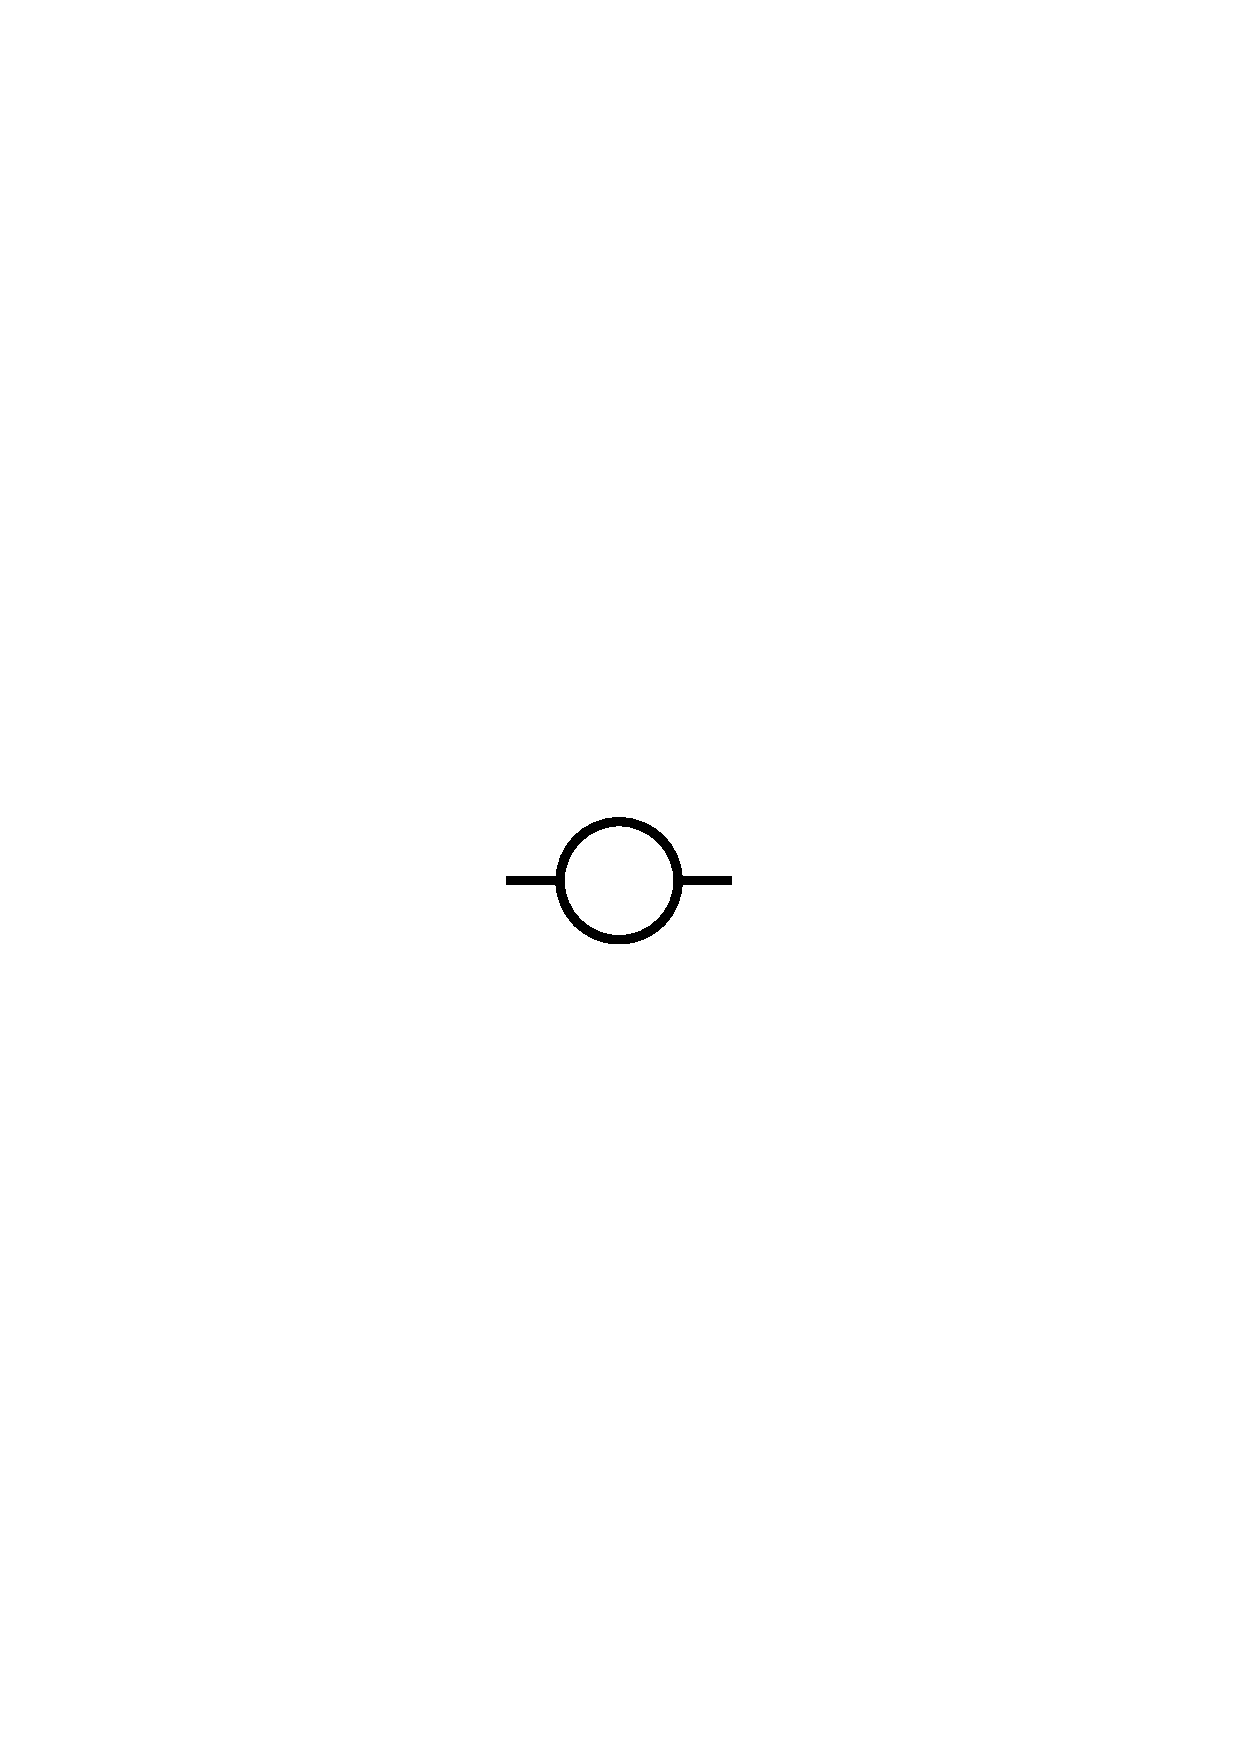
\includegraphics[width=0.5\textwidth]{ch3_loopamps/figures/topo-bub.pdf}
    \label{fig:topo-bub}
    \caption{bubble}
  \end{subfigure}
  \hfill
  \begin{subfigure}{0.4\textwidth}
    \hspace*{0.17\textwidth}
    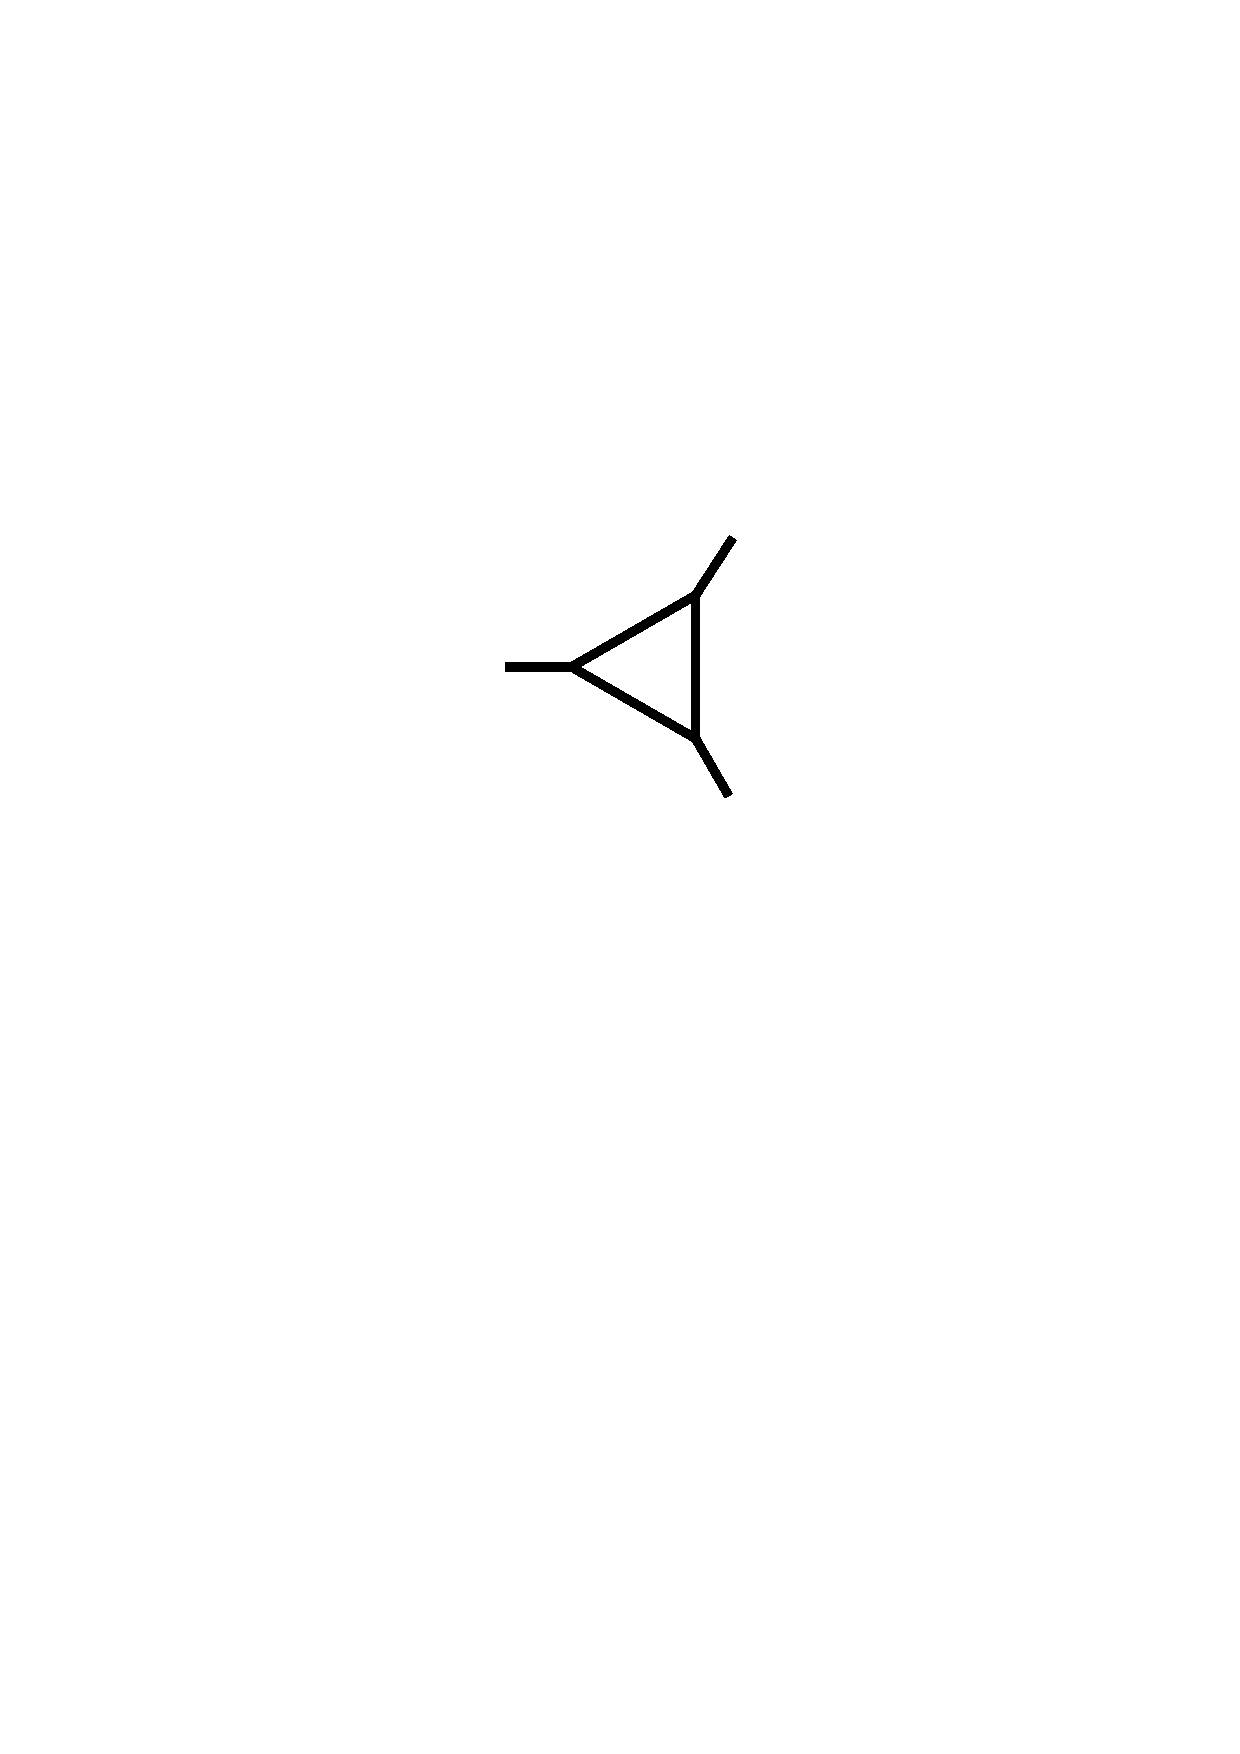
\includegraphics[width=0.5\textwidth]{ch3_loopamps/figures/topo-tri.pdf}
    \label{fig:topo-tri}
    \caption{triangle}
  \end{subfigure}
  \\
  \begin{subfigure}{0.4\textwidth}
    \centering
    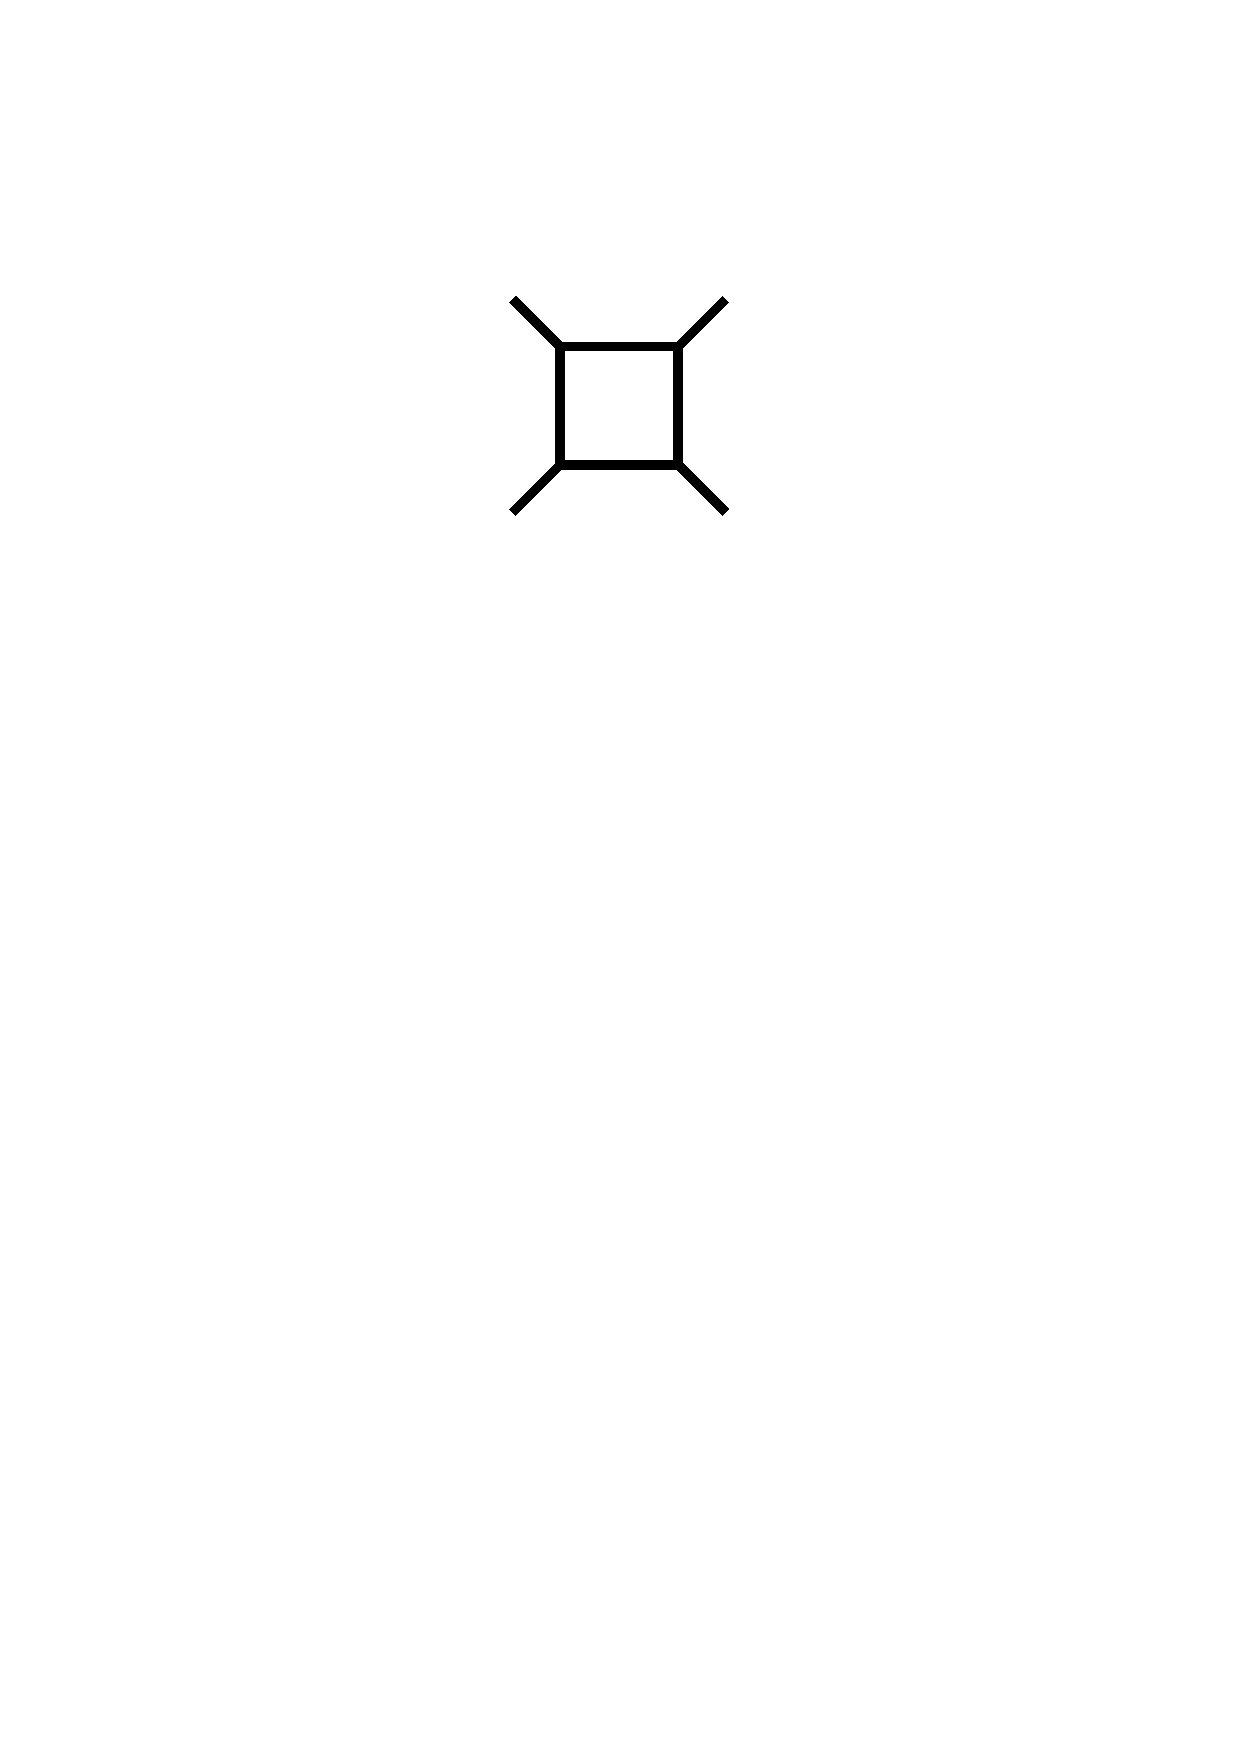
\includegraphics[width=0.5\textwidth]{ch3_loopamps/figures/topo-box.pdf}
    \label{fig:topo-box}
    \caption{box}
  \end{subfigure}
  \hfill
  \begin{subfigure}{0.4\textwidth}
    \centering
    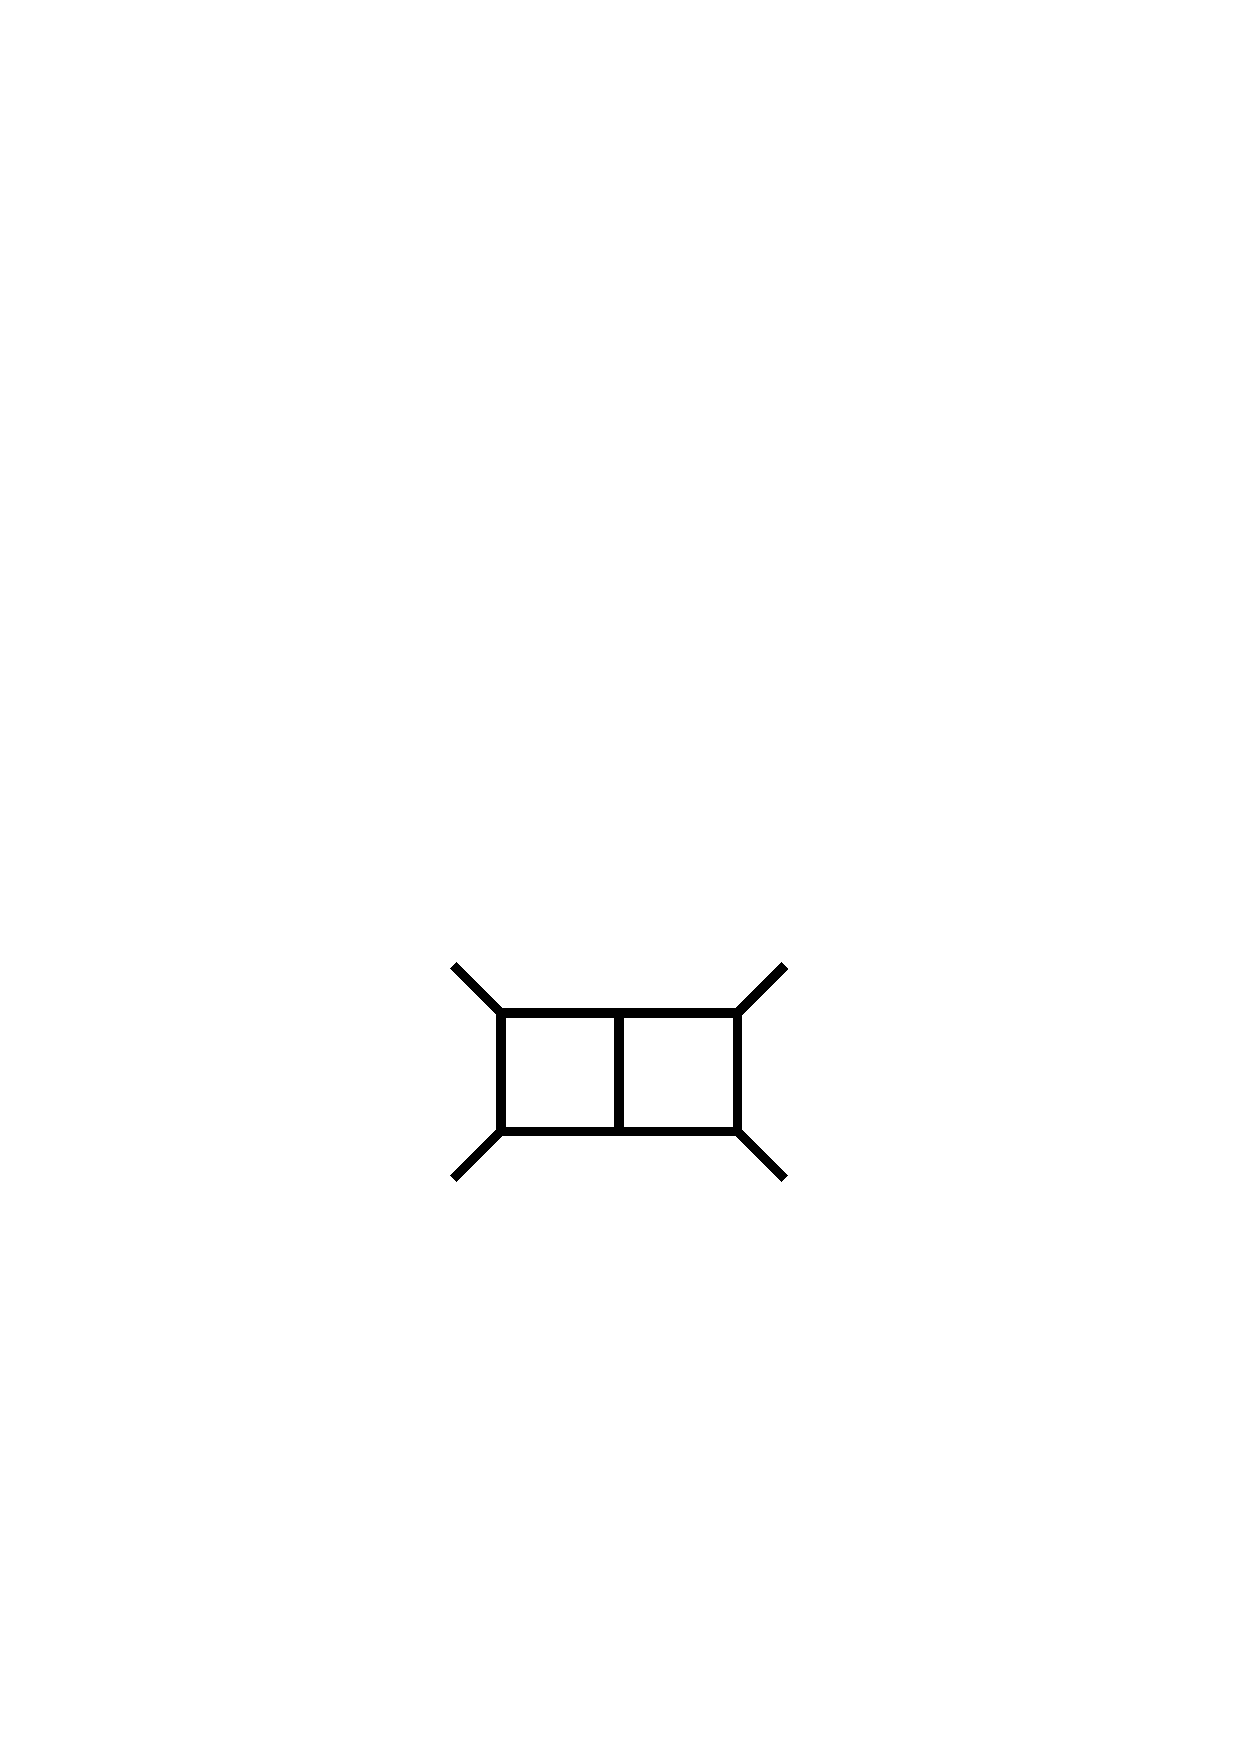
\includegraphics[width=0.74\textwidth]{ch3_loopamps/figures/topo-dblbox.pdf}
    \label{fig:topo-dblbox}
    \caption{two-loop double box}
  \end{subfigure}
  \caption{Example loop topology graphs.}
  \label{fig:topo}
\end{figure}

At one loop all topologies take the form of an $n$-gon with a potential numerator function $N$,
\begin{equation}
  F_n^{(1),[D]}[N] = \int_k \frac{N}{\prod_{a=1}^{n}\bigl[-(k-q_a)^2+m_{a}^2-\i0\bigr] } \,,
  \label{eq:oneloopintegraldef}
\end{equation}
where $q_a = \sum_{b=1}^{a-1} p_b$ (with $q_1 = 0$) are the momenta flowing in
each propagator, which also have a mass $m_{a}$. We have also introduced a
short hand for the integration measure:
\begin{equation}
  \int_k \coloneqq \int \frac{\d^D k}{\i \pi^{D/2}} \,.
\end{equation}
Note the different loop integration measure with respect to the $\d^D k/(2\pi)^D$ in the Feynman rules. This difference is responsible for the factors of $\i$ and $\pi$ in \eqn{eq:loopamp-general}, and will be motivated in section~\ref{sec:introduction}.
The configuration of momenta and propagators of \eqn{eq:oneloopintegraldef} is shown graphically in figure~\ref{fig:onelooppic}. Cases in which the numerator
is one, $F_n^{(1),[D]}[1]$, are referred to as \emph{scalar integrals}. When
using an integer $n$ to represent the topology we are already indicating that
it is a one-loop integral, and so the loop-order superscript will be dropped for
the remainder of this chapter. If no numerator is specified it should
considered to be a scalar integral and so $F_n^{[D]} \equiv F_n^{[D]}[1] \equiv
F_n^{(1),[D]}[1]$. A small imaginary part $\i0$ follows from the Feynman
prescription for the propagators that was introduced in the Feynman rules.
This $\i0$ prescription will mainly play a role only when evaluating the
integrals, and so we will drop it from the propagator expressions in cases where
it is not necessary. We will follow the standard convention to refer to the
simple one-loop topologies according to the polygon that represents the number of
propagators, e.g.\ bubble for two propagators, triangle for three propagators,
box for four propagators, and so on (see figure ~\ref{fig:topo} again). An integral with one propagator is
referred to as a tadpole integral.

\begin{figure}[t]
\centering
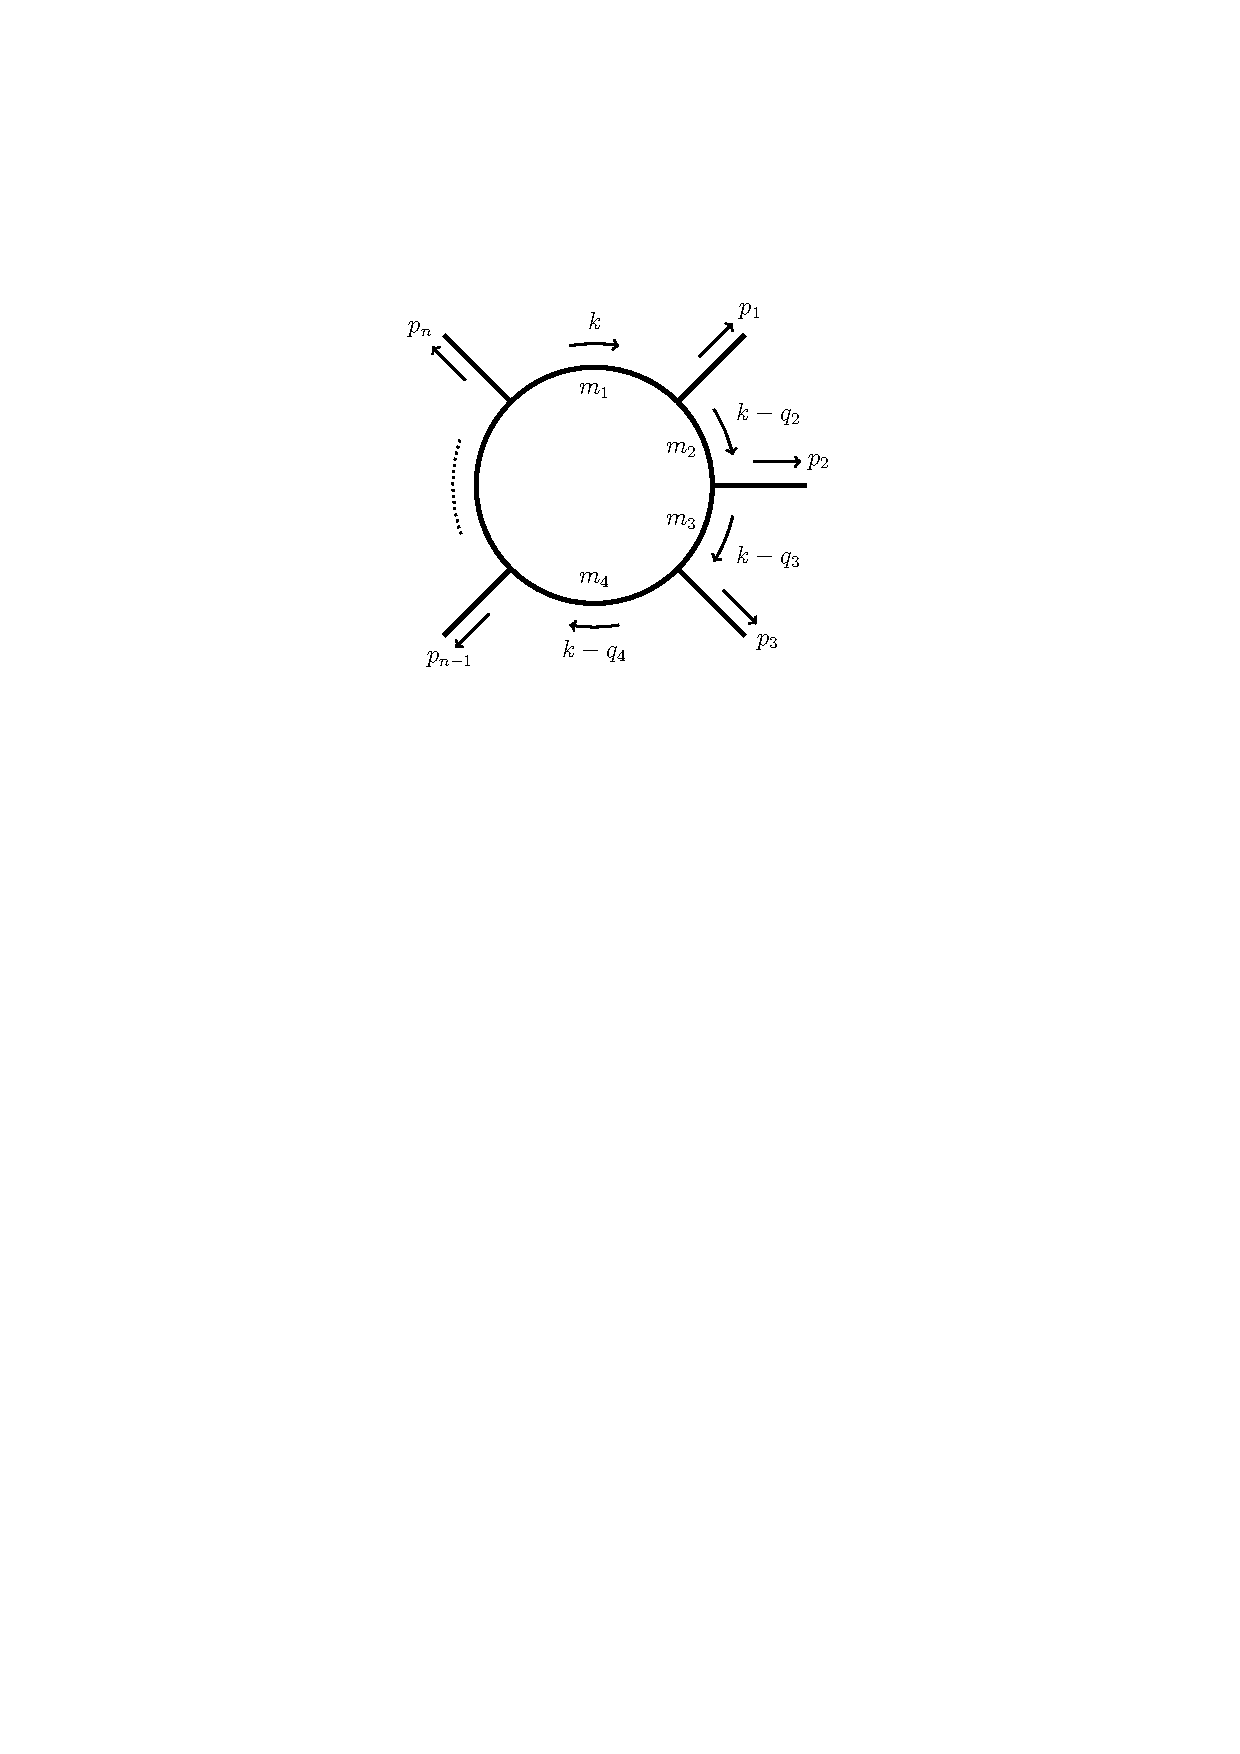
\includegraphics[width=0.5\textwidth]{ch3_loopamps/figures/1Lintegral-notation.pdf}
\caption{The generic one-loop integral.}
\label{fig:onelooppic}
\end{figure}

The coefficients of the integrals in \eqn{eq:loopamp-general} can be expanded around the physical space-time dimension $D=4$, as
\begin{equation}
  c_T^{[D]} = c_T^{(0)} + \eps \, c_T^{(1)} + \eps^2 \, c_T^{(2)} + \ldots
  \label{eq:coeffexp}
\end{equation}
The order at which we must expand the coefficients to ensure the correct result
for the amplitudes as $\eps\to 0$ will depend on the overall divergences present
in the loop integrals.

We may also consider the \emph{integrand} of an amplitude $A_n^{(L),[D]}(1,\ldots,n)$, which we denote $I_n^{(L),[D]}(1,\ldots,n)$, and is a rational function satisfying
\begin{equation}
  A_n^{(L),[D]}(1,\ldots,n) = \int \prod_{l=1}^L \frac{\d^D k_l}{\i\pi^{D/2}} \, I_n^{(L),[D]}(k, 1,\ldots,n) \,.
\end{equation}
The amplitude integrands are not uniquely defined, as they may differ by terms which integrate to zero, thus giving rise to the same amplitude. The simplest choice is to use the Feynman-diagram expansion to define the integrand.
If we make the assumption that a colour-ordered one-loop amplitude has a single
ordering of the external legs for the topology with $n$ propagators (this is the case for the
leading-colour approximation in Yang-Mills theory), we can be more explicit and
write
\begin{equation} \label{eq:integrand_ordered_1L}
  I_n^{(1),[D]}(k,1,\ldots,n) = \frac{{N}(k,1,\ldots,n)}{\prod_{a=1}^{n}\bigl[-(k-q_a)^2+m_{a}^2-\i0\bigr]} \,.
\end{equation}
In the same way that we can try to find a basis of Feynman integrals for the
amplitude, we may also ask if there exists a basis of loop-momentum dependent
numerator functions $\{f_x\}$ such that the integrand numerator in \eqn{eq:integrand_ordered_1L} can be written as
\begin{equation}
  N(k,1,\ldots,n) = \sum_x c_x(1,\ldots,n) \,f_x(k,p_1,\ldots,p_{n-1}) \,,
\end{equation}
where the coefficients $c_x$ are rational functions of the external kinematics,
and $f_x$ are independent scalar products dependent on the loop momentum.
Again, the sum over $x$ and the definition of ``independent'' here are not yet
defined but we can motivate the construction with a simple example. If we
consider a one-loop integrand $I_n^{(1),[D]}(k,1,2,3)$ in which
${N}(k,1,2,3) = k\cdot q_{2}$, then we can express the numerator in terms of
the difference of two propagators in order to rewrite everything in terms of scalar integral
functions:
\begin{eqnarray}
  \begin{aligned}
  {N}(k,1,2,3)
  &= \frac{1}{2}\left[ \bigl(-(k-q_2)^2+m_2^2\bigr) - \bigl(-k^2+m_1^2\bigr) + q_2^2-m_2^2+m_1^2 \right] \\
  &= \frac{1}{2}\left\{1,-1,q_2^2-m_2^2+m_1^2\right\} \cdot \left\{-(k-q_2)^2+m_2^2, -k^2+m_1^2, 1\right\}^{\top} \,.
  \end{aligned}
\end{eqnarray}
So in this case the functions $f_x$ are the inverse propagators and $1$.

Throughout this chapter we will use the example of four-gluon scattering to
illustrate general methods for loop integrands and amplitudes. Sample diagrams
for this process are shown in figure~\ref{fig:4gluon1L}. In this case the most
complicated topology is the box graph which, following the structure of
the three-gluon vertex, has a maximum of four powers of the loop momentum
in the numerator function. Graphs containing vertex corrections or those with
bubble insertions will contain triangle and bubble tensor integrals
respectively. As we will see, writing the loop-momentum dependence of the numerator in terms of
the propagators in each graph will allow us to find a basis of scalar Feynman
integrals, so that the particular form of \eqn{eq:loopamp-general} relevant for four-gluon scattering becomes
\begin{align}
\begin{aligned}
  A_4^{(1),[D]}&(1,2,3,4) =
  \i \, c_{{\rm box}}^{[D]} \, F_{4}^{[D]}[1](p_1,p_2,p_3) \\&
  %
  + \i \, c_{{\rm tri},1}^{[D]} \, F_{3}^{[D]}[1](p_1,p_2)
  + \i \, c_{{\rm tri},2}^{[D]} \, F_{3}^{[D]}[1](p_1,p_{23}) \\&
  + \i \, c_{{\rm tri},3}^{[D]} \, F_{3}^{[D]}[1](p_{12},p_3)
  + \i \, c_{{\rm tri},4}^{[D]} \, F_{3}^{[D]}[1](p_2,p_3) \\&
  %
  + \i \, c_{{\rm bub},1}^{[D]} \, F_{2}^{[D]}[1](p_{12})
  + \i \, c_{{\rm bub},2}^{[D]} \, F_{2}^{[D]}[1](p_{23}) \,.
 \end{aligned}
\end{align}
where we have used the notation,
\begin{equation}
  p_{i_1 \cdots i_n} = p_{i_1} + p_{i_2} + \cdots + p_{i_n},
\end{equation}
which will also be used for the invariants,
\begin{equation}
  s_{i_1 \cdots i_n} = p_{i_1\cdots i_n}^2.
\end{equation}
The fact that only scalar integrals appear remains to be proven of course. We
will also set about the task of extracting the coefficients of these scalar
integrals and the task of generalising to the $n$-point case.

\begin{figure}[t!]
  \centering
  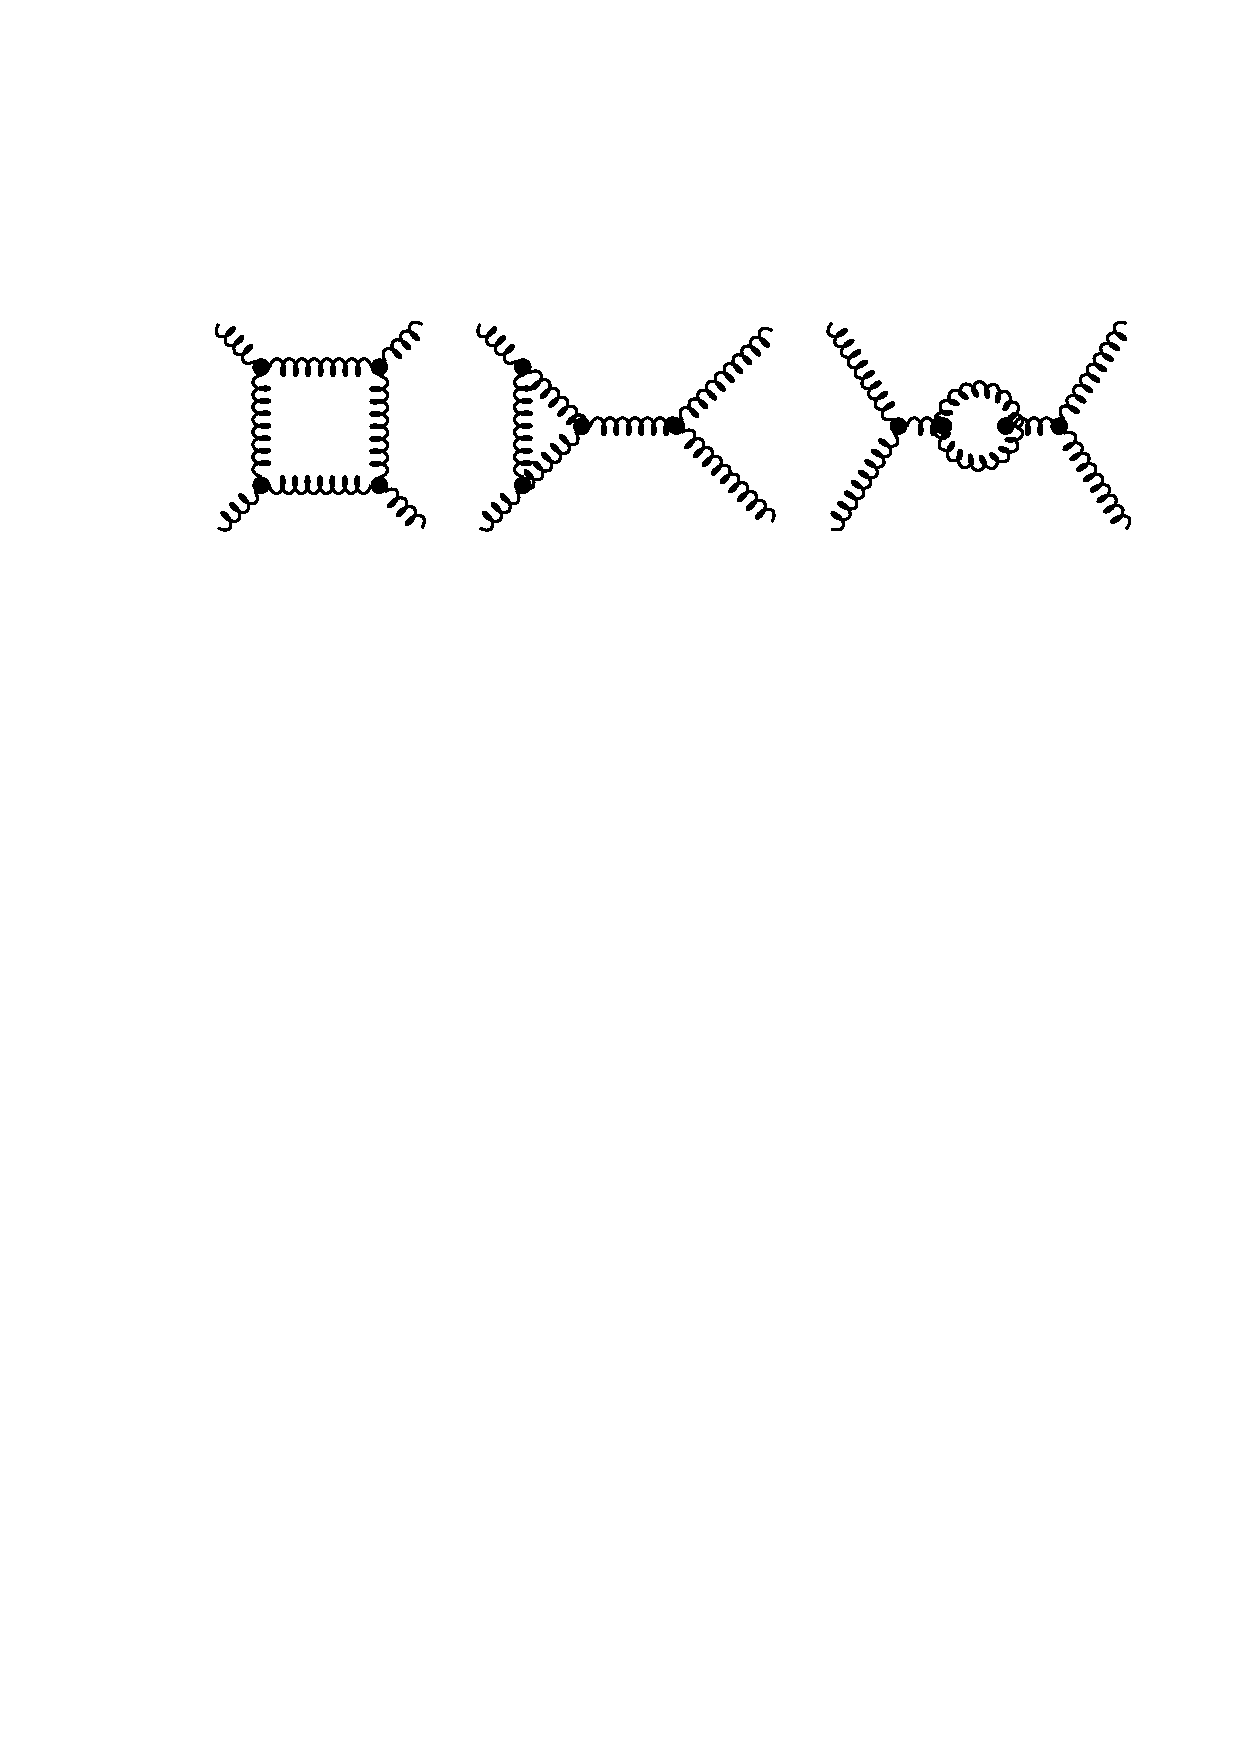
\includegraphics[width=0.8\textwidth]{ch3_loopamps/figures/4gfdiags.pdf}
  \caption{Sample diagrams contributing to the four-gluon scattering amplitude at one-loop order.}
  \label{fig:4gluon1L}
\end{figure}

The chapter is organised as follows. We start in section~\ref{sec:3.2} by
demonstrating that the unitarity of the $S$-matrix leads to deep insights into
the structure of loop amplitudes. This will lead us to consider the
discontinuities of loop amplitudes, and show that they may be computed from the
product of tree-level amplitudes. Using the example of four-gluon scattering, we will demonstrate that this results in an extremely efficient technique to
identify simple integral structure in the amplitude. We will then explore
generalised discontinuities of loop amplitudes in section~\ref{sec:3.3}, and use
the ``Cutkosky rules'' to make a direct connection with the pole structure of the
integrand. The factorisation on these poles leads to the generalised unitarity
method, which allows for the computation of the coefficients of the
scalar box integrals. Section~\ref{sec:3.4} lays the ground work for the
general treatment of any loop amplitude, as we use tensor reduction and
integrand-level analysis of transverse spaces to identify relations between
Feynman integrals. Section~\ref{sec:3.5} is dedicated to the derivation of the
complete decomposition of a general one-loop amplitude into a basis of scalar
integrals, and how their coefficients may be extracted from products of
tree-level amplitudes via generalised unitarity. In section~\ref{sec:rat4g} we
put all of this technology to work to complete the computation of the one-loop four-gluon scattering amplitude
in dimensional regularisation. Finally we give some outlook and extensions of
the ideas presented here, and consider efficient computations using rational
parametrisations of the external kinematics in section~\ref{sec:3.7} and
extensions to two-loop integrands in section~\ref{sec:3.8}.

Further information on the topics presented in this chapter can be found in a number of comprehensive reviews, for example see~\cite{ch3_Dixon:1996wi,ch3_Dixon:2013uaa,ch3_Ellis:2011cr}.

\begin{svgraybox}
  \textbf{Ultraviolet power counting.}
  Before we get started with the main topics of this chapter it is useful to recall how we can quantify UV divergences.
  The divergences at large values of the loop momentum can be estimated at the integrand level by considering the
  scaling behaviour. For example, using general polar coordinates, one-loop scalar integrals become
  \begin{equation} \label{eq:UVpowercounting}
    F_n^{[D]}[1] \overset{|k|\to\infty}{\to} \int \frac{(-1)^n |k|^{D-1} \d |k| \, \d\Omega}{\i\pi^{D/2}} \frac{1}{k^{2n}} \,,
  \end{equation}
  from which we see a divergence if $n\leq D/2$. If $n=2$ in $D=4-2\eps$, we have that
  \begin{equation}
    F_{2}^{[4-2\eps]}[1] \overset{|k|\to\infty}{\to} \int \frac{\d |k| \, \d\Omega}{\i\pi^{2-\eps}} \frac{1}{|k|}\,,
    \label{eq:UVcountingbubble}
  \end{equation}
  and we see a logarithmic divergence. Infrared divergences, such as the soft
  and collinear configurations discussed in chapter~\ref{ch:trees}, are more difficult to
  classify but can also be regulated by the analytic continuation of the
  dimension. We will discuss this further in chapter~\ref{ch:loopints}, where we focus on the
  integration over loop momenta. 
\end{svgraybox}

\section{Unitarity and cut construction \label{sec:3.2}}

The unitarity of the $S$-matrix provides some of the most fundamental
constraints on the analytic form of on-shell amplitudes. 
The initial steps
follow the discussion of the optical theorem and Cutkosky analysis of the
discontinuities of Feynman integrals~\cite{ch3_Cutkosky:1960sp} that may be familiar to many readers.

The scattering amplitudes associated with an $S$-matrix  $S = \1 + \i T$ are
determined through the transition matrix $T$. Transition matrix elements
$\langle F | T | I \rangle$ are a measure of the probability of a initial state $I$
evolving into a final state $F$. 

The unitarity condition of the $S$-matrix
\begin{equation}
  S^\dagger S = \1
  \end{equation}
implies a non-linear constraint on the transition matrix:
\begin{align}
 - \i \bigl(T-T^\dagger \bigr) =  T^\dagger T  \,.
  \label{eq:Sunitarity}
  \end{align}
The asymptotic states obey the completeness relations
\begin{equation} 
  \sum_{n} \int \prod_{j=1}^n \frac{\d^3 \vec{k}_j}{(2\pi)^3 \, 2 E_j} \ |\{k\}_n \rangle\langle \{k\}_n | = \1 \,,
\end{equation}
where $|\{k\}_n  \rangle$ indicate multi-particle states $|\{k\}_j\rangle
\coloneqq |k_1,k_2, \ldots,k_n\rangle$, $k_i^{\mu} = ( E_i, \vec{k}_i)$, and
$E_i^2 = |\vec{k}_i|^2 + m_i^2$, $m_i$ being the mass of the $i$th particle. Therefore,
when we contract \eqn{eq:Sunitarity} with the initial and final states
and insert a complete set of states in the product $T T^\dagger$, we determine
that
\begin{equation}
  -\i\langle F| \bigl(T-T^\dagger\bigr)|I\rangle =
  \sum_{n} \int \prod_{j=1}^n \frac{\d^3 \vec{k}_j}{(2\pi)^3 \, 2 E_j} \,\langle F| T^\dagger|\{k\}_n\rangle \,\langle \{k\}_n |T|I\rangle \,.
  \label{eq:unitarity-Tmatexp}
\end{equation}

The scattering amplitude $A(I\to F)$ is extracted from the transition matrix
element stripped of the overall momentum-conserving delta function. If we represent
this amplitude by a picture,
\begin{align}
  A(I \to F) = \raisebox{-0.4cm}{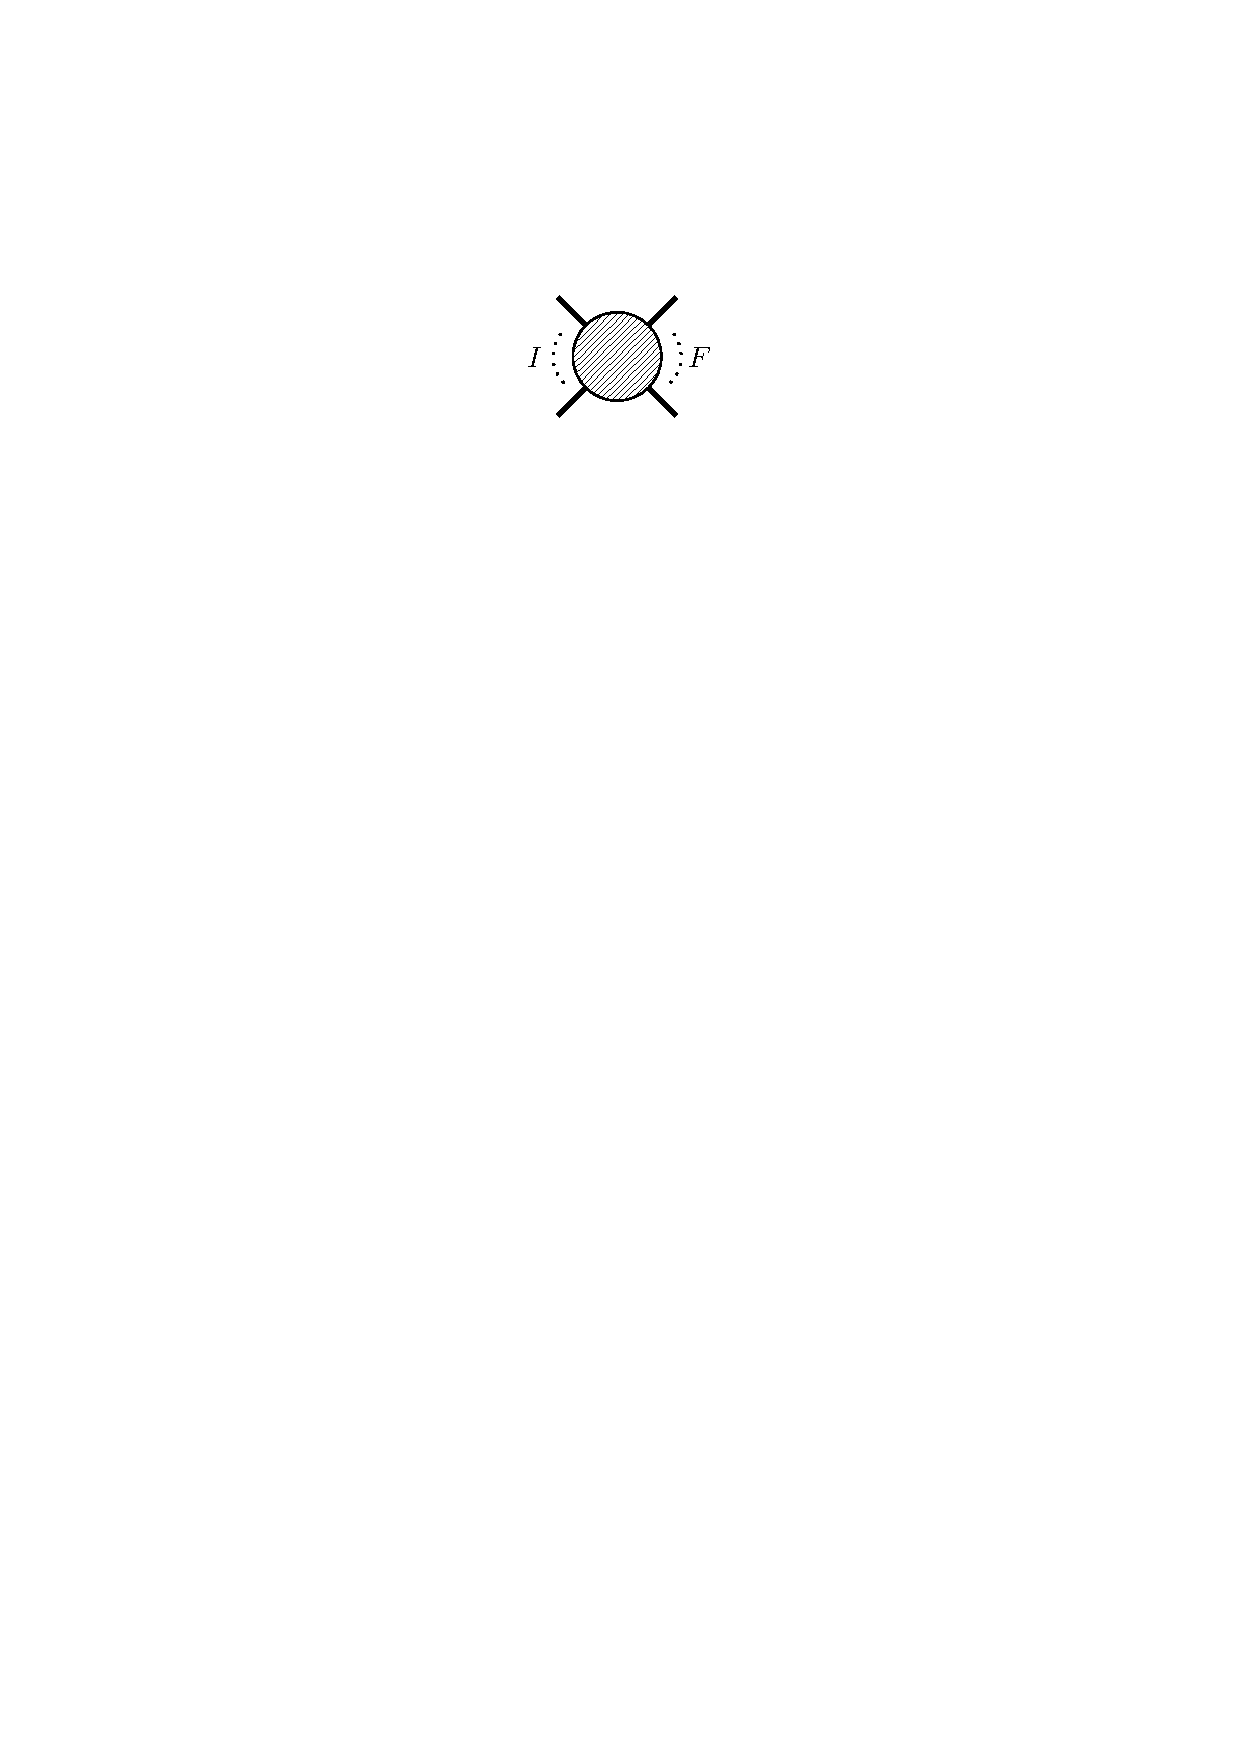
\includegraphics[width=1.5cm]{ch3_loopamps/figures/ampIFall.pdf}} \,,
\end{align}
we can show the relation \eqref{eq:unitarity-Tmatexp} graphically, as
\begin{align} \begin{aligned}
  -2\i \left(
       \raisebox{-0.4cm}{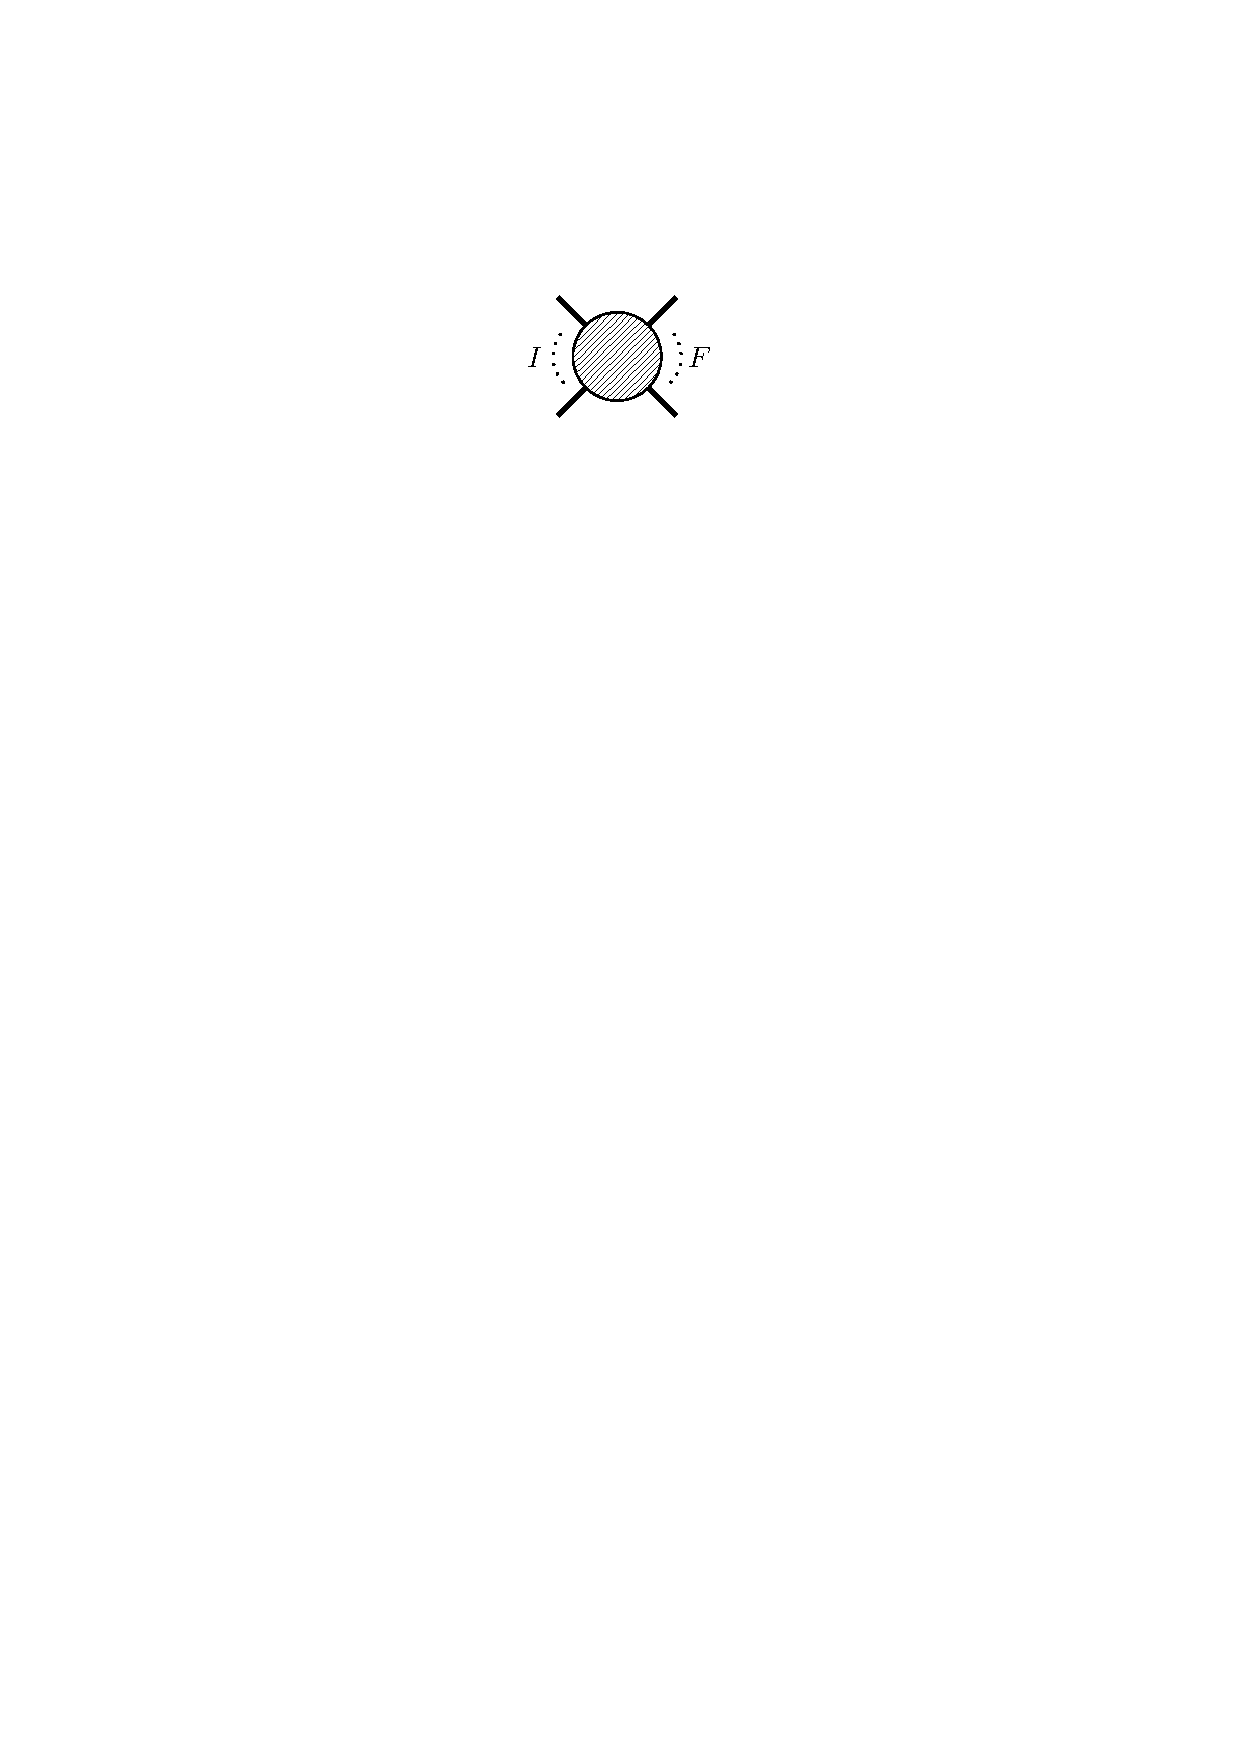
\includegraphics[width=1.5cm]{ch3_loopamps/figures/ampIFall.pdf}}
     - \raisebox{-0.4cm}{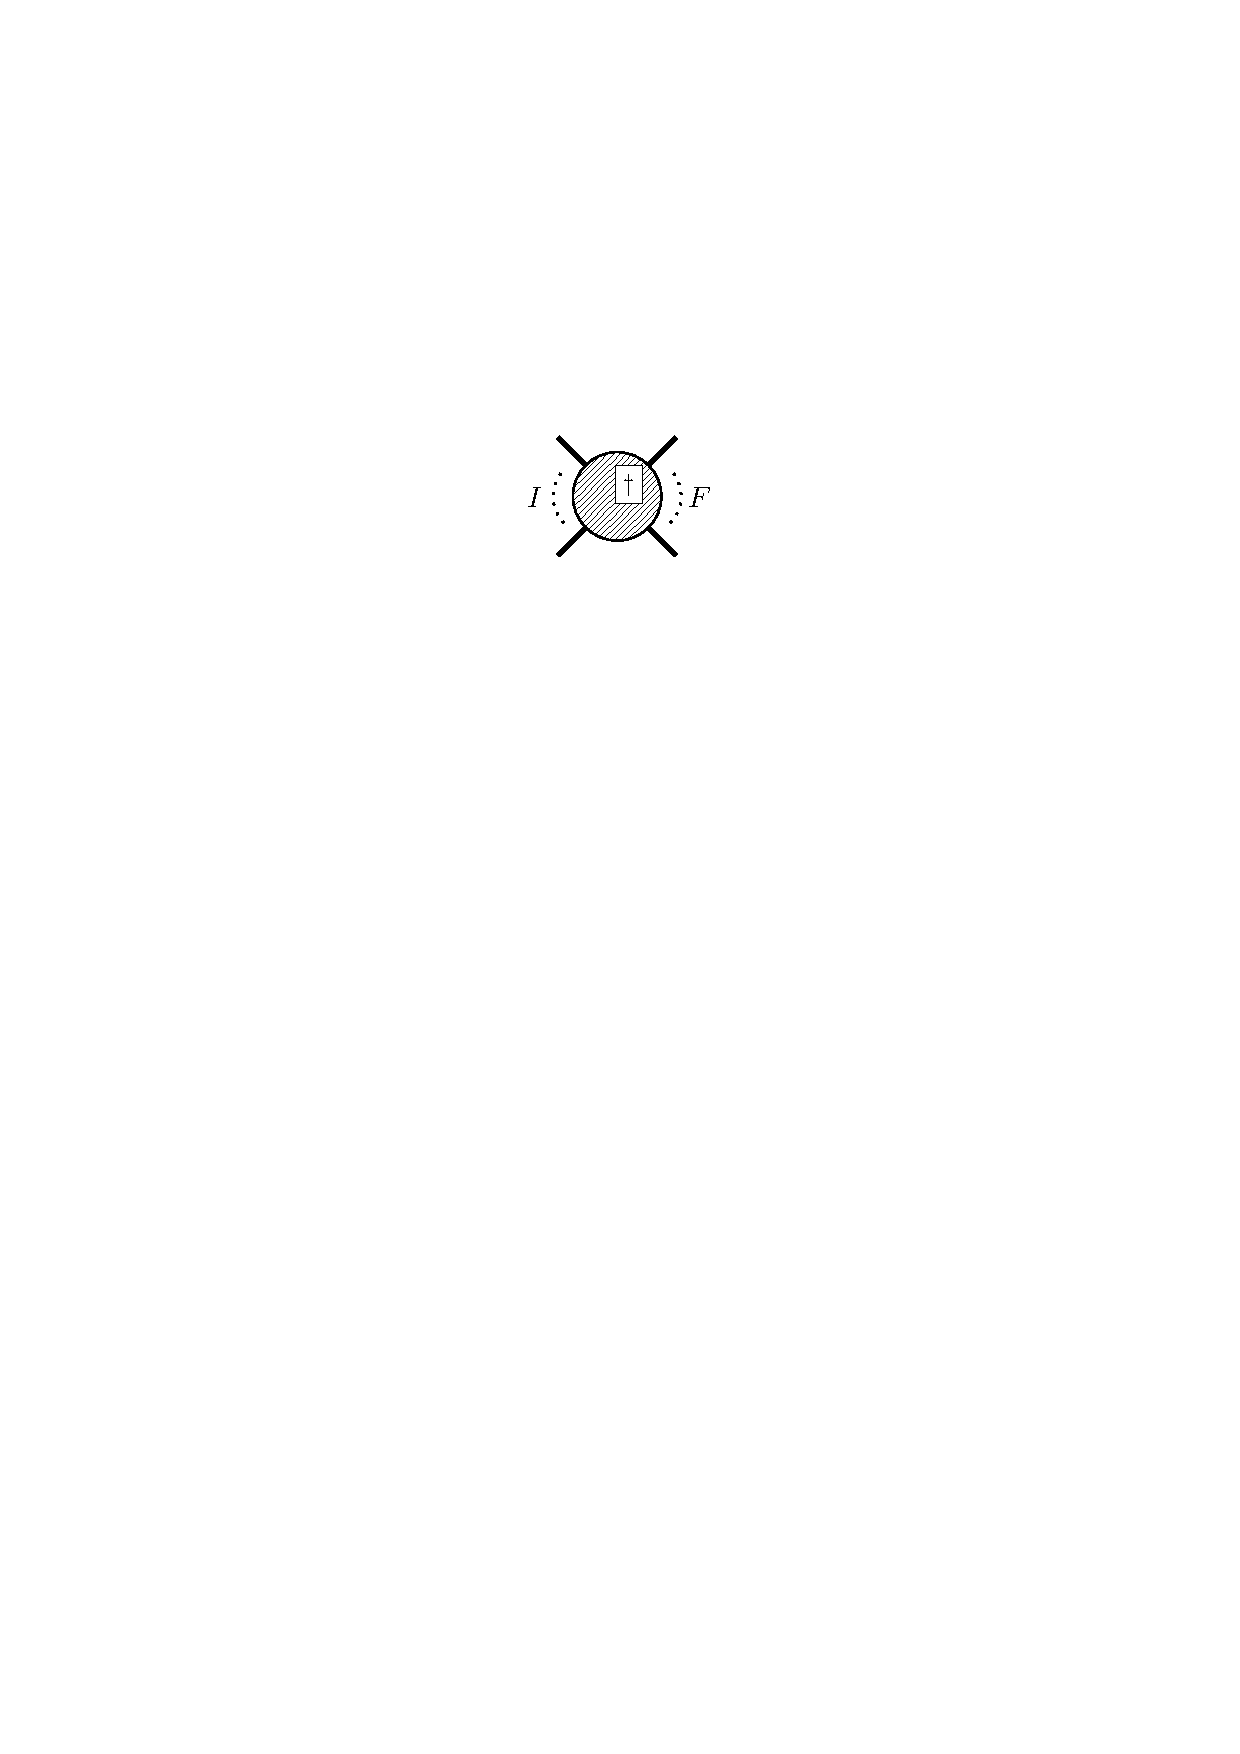
\includegraphics[width=1.5cm]{ch3_loopamps/figures/ampFIall.pdf}}
  \right)
  &= \sum_{n=2}^{\infty} \int \d\Phi_n(P, \{k\}_n) \raisebox{-0.4cm}{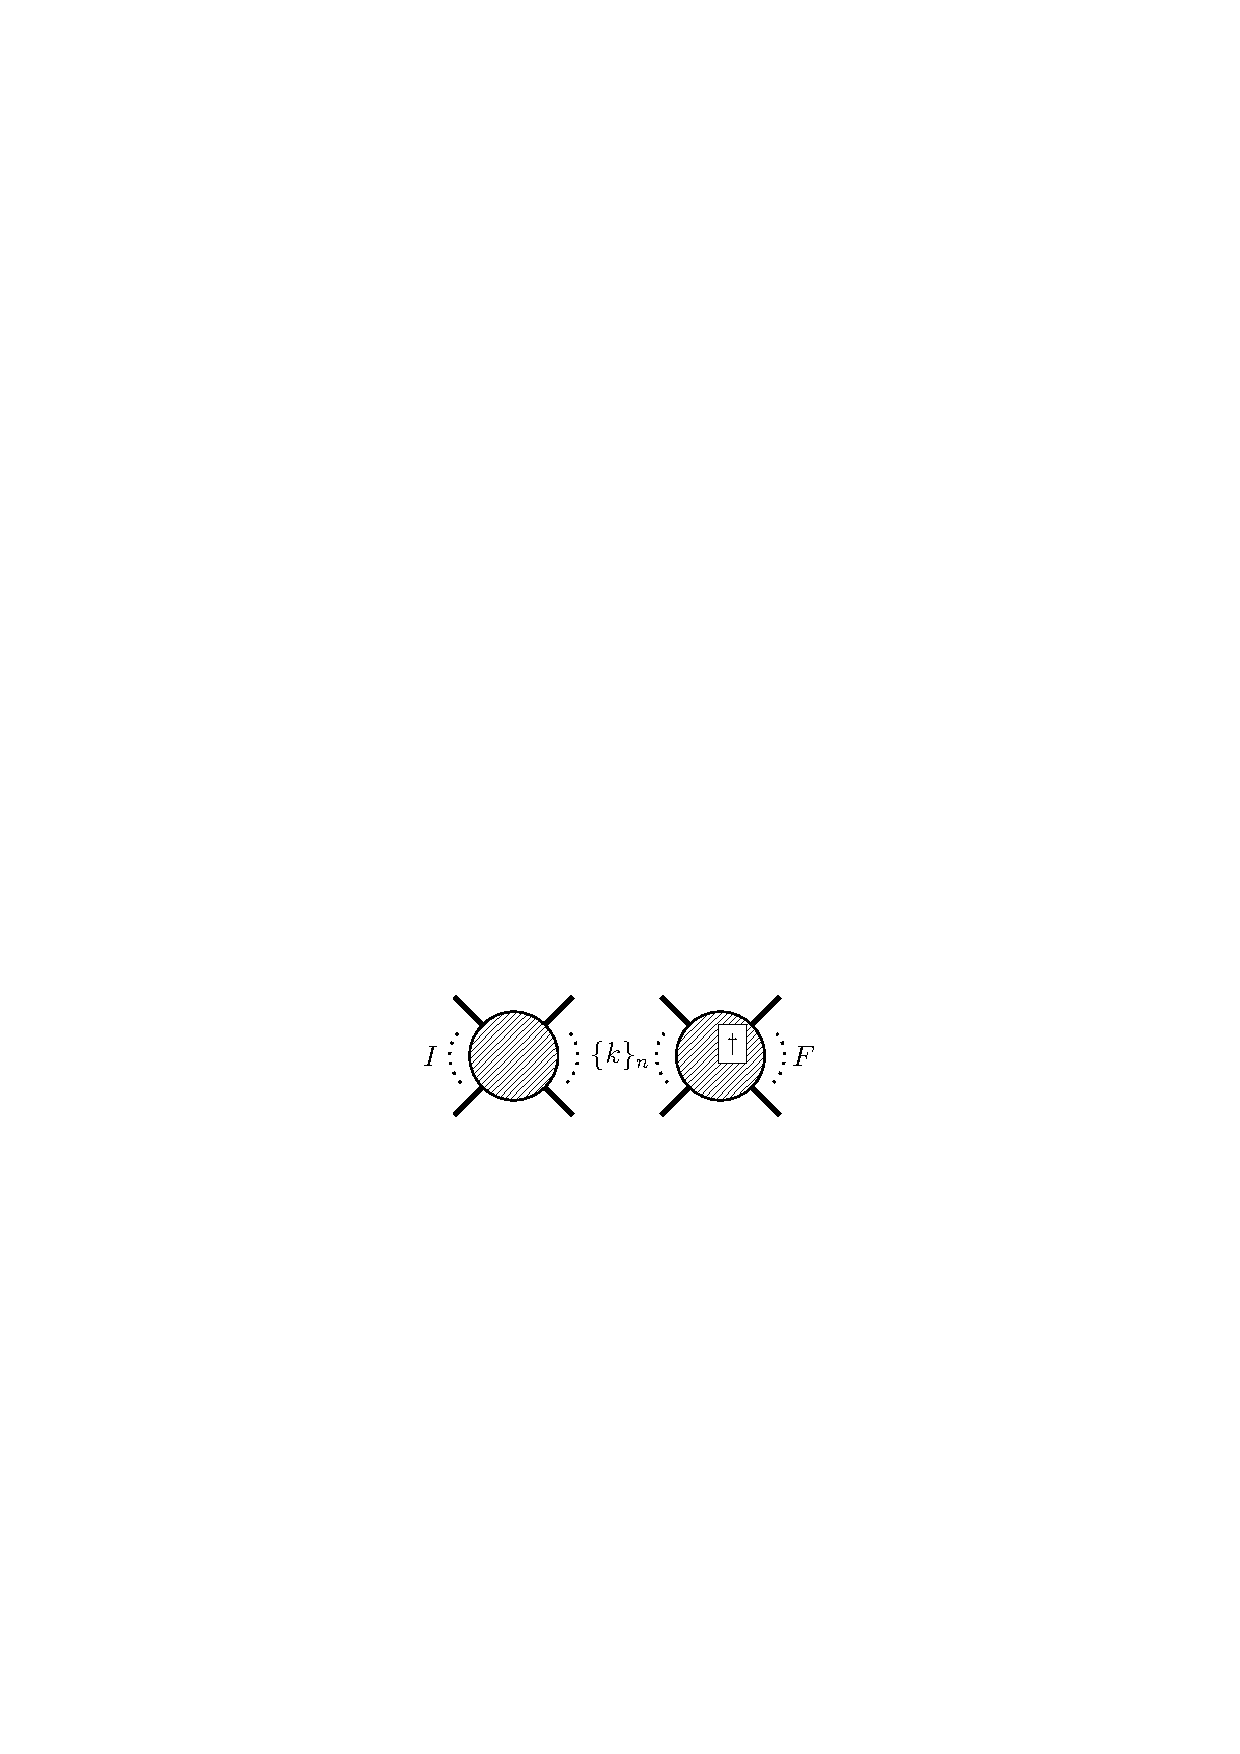
\includegraphics[width=3cm]{ch3_loopamps/figures/ampIkkFall.pdf}}\,,
  \end{aligned}
  \label{eq:unitarity-pictorial}
\end{align}
where the integration measure now includes the on-shell delta function that ensures an on-shell final state phase-space integral,
\begin{align}
  \d\Phi_n(P, \{k\}_n) = (2\pi)^4 \delta^{(4)}\left( P-\sum_n k_n \right) \prod_{i=1}^n \frac{\d^3 \vec{k}_i}{(2\pi)^3 \, E_i}.
  \label{eq:phase_space}
\end{align}
The momentum $P$ above represents the total incoming momentum $P = \sum_i p_i$.

The LHS of \eqn{eq:unitarity-pictorial} may be shown to be
proportional to the discontinuity of the amplitude across the real $P^2$ axis.
While we will not see any specific examples until chapter~\ref{ch:loopints}, Feynman integrals
will in general contain branch cuts. The simplest function of this type is the
logarithm $\log(x)$,\footnote{We saw the logarithm appear in the UV limit of of
the one-loop bubble function $F_{2}^{[4-2\eps]}[1]$ in \eqn{eq:UVcountingbubble}.} which
has a branch cut across the (negative) real $x$ axis. For a generic function
$f(x)$, the discontinuity across the real $x$ axis is defined as ${\rm
Disc}_{x} f(x) \coloneqq  f(x+\i0) - f(x-\i0)$. For the logarithm this gives
${\rm Disc}_{x} \log(x) = 2\pi \i \, \Theta(-x)$, where $\Theta(-x)$ is the
Heaviside step function (for further details see exercise~\ref{Ex:Discontinuities}).
Rational functions, such as the tree-level amplitudes we have encountered up
until now, do not contain branch cuts. We can take the unitarity constraint to
imply that scattering amplitudes do contain branch cuts. Following this
argument, it is possible to show that
\begin{align} \begin{aligned}
  -2\i \left(
       \raisebox{-0.4cm}{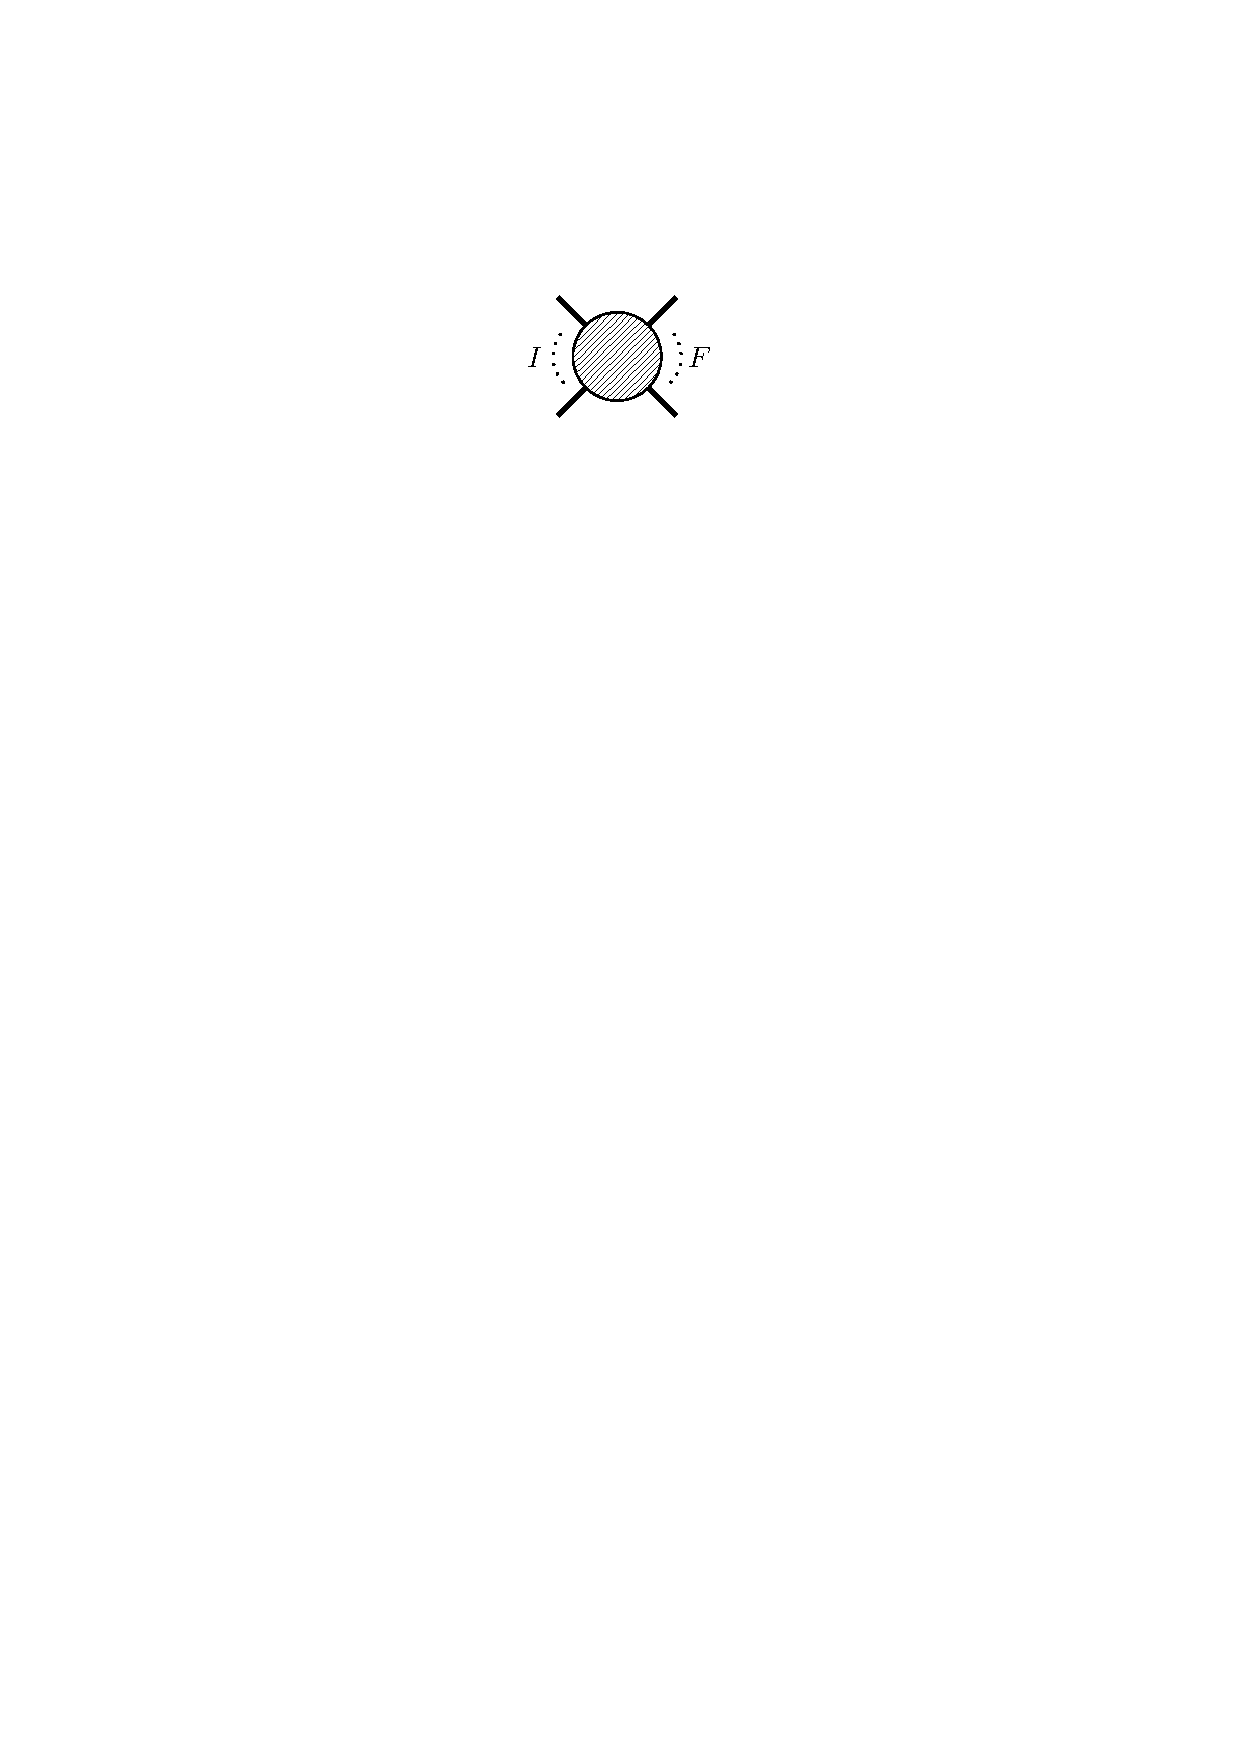
\includegraphics[width=1.5cm]{ch3_loopamps/figures/ampIFall.pdf}}
     - \raisebox{-0.4cm}{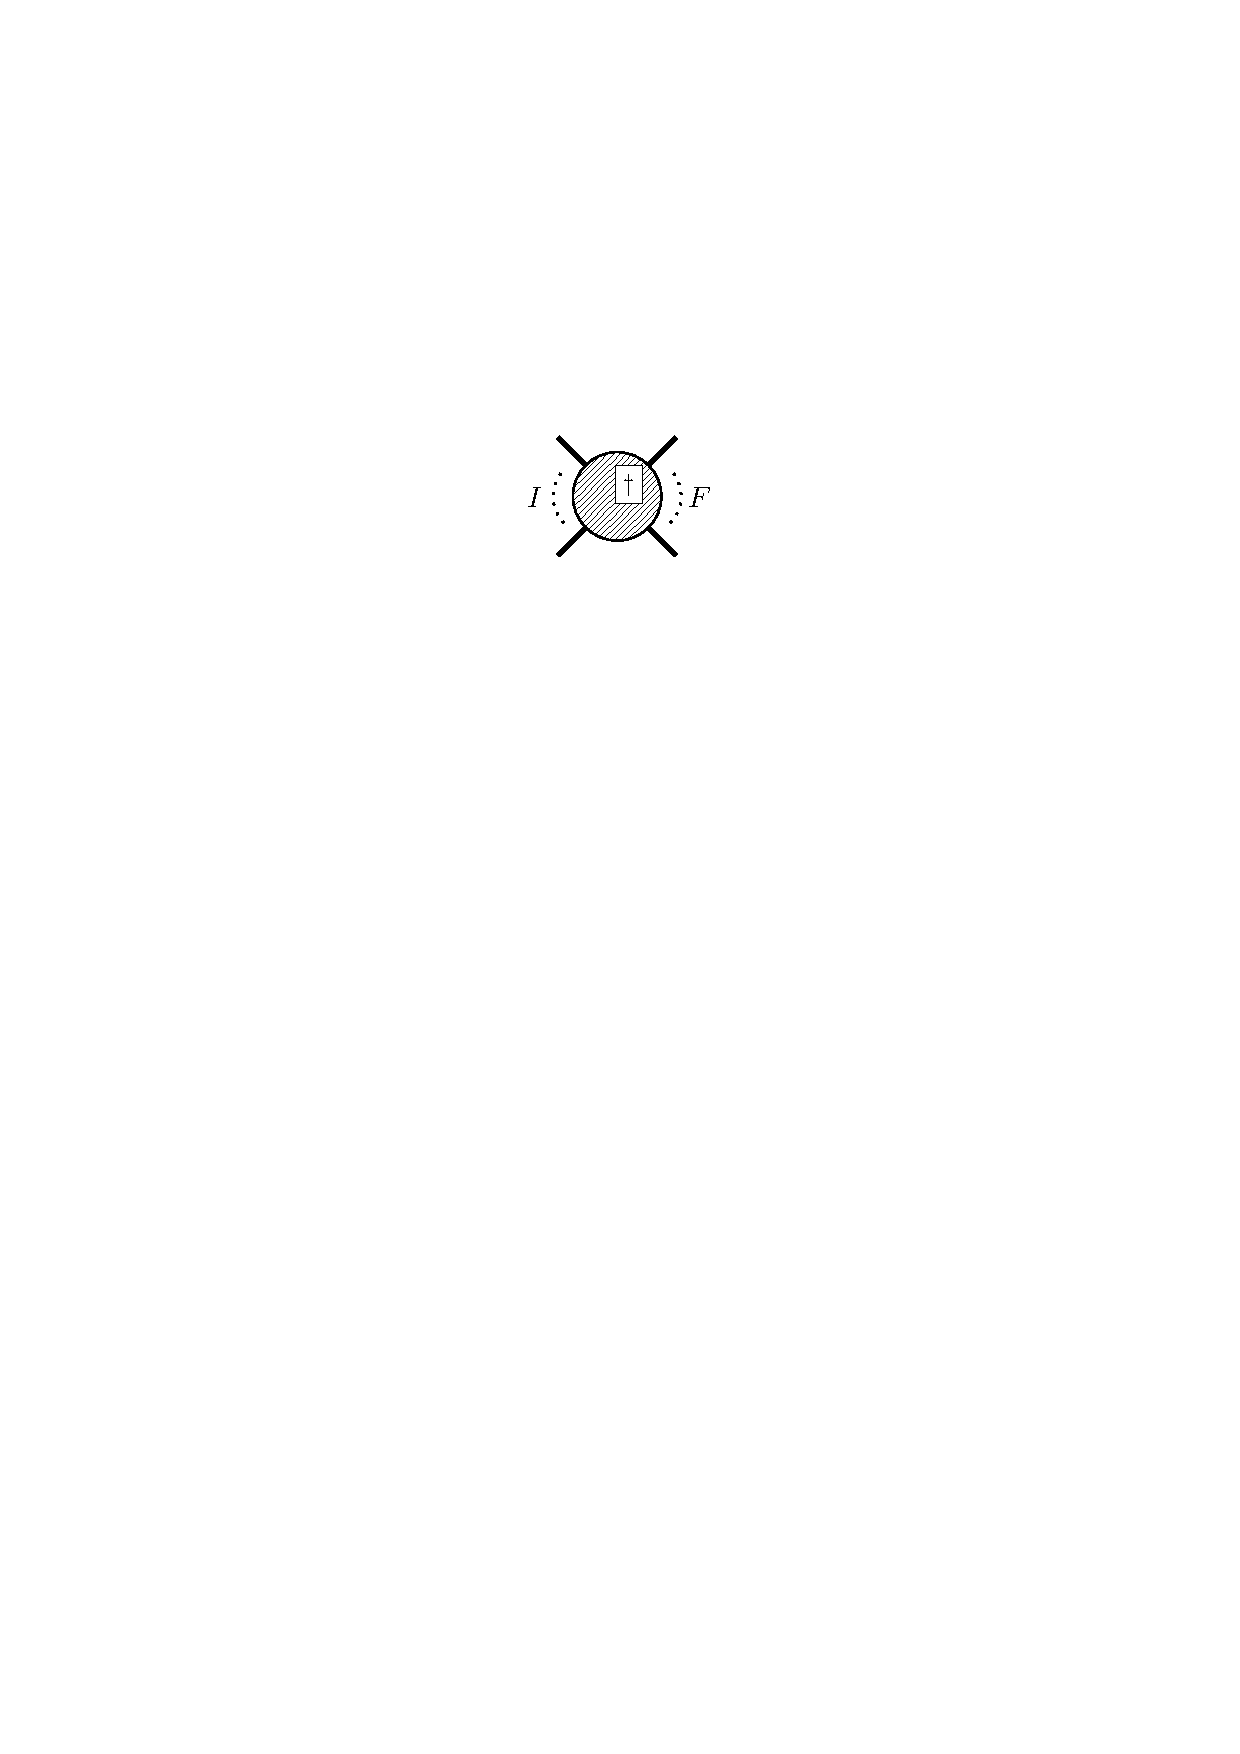
\includegraphics[width=1.5cm]{ch3_loopamps/figures/ampFIall.pdf}}
  \right)
  &= {\rm Disc}_{P^2}\left( \raisebox{-0.4cm}{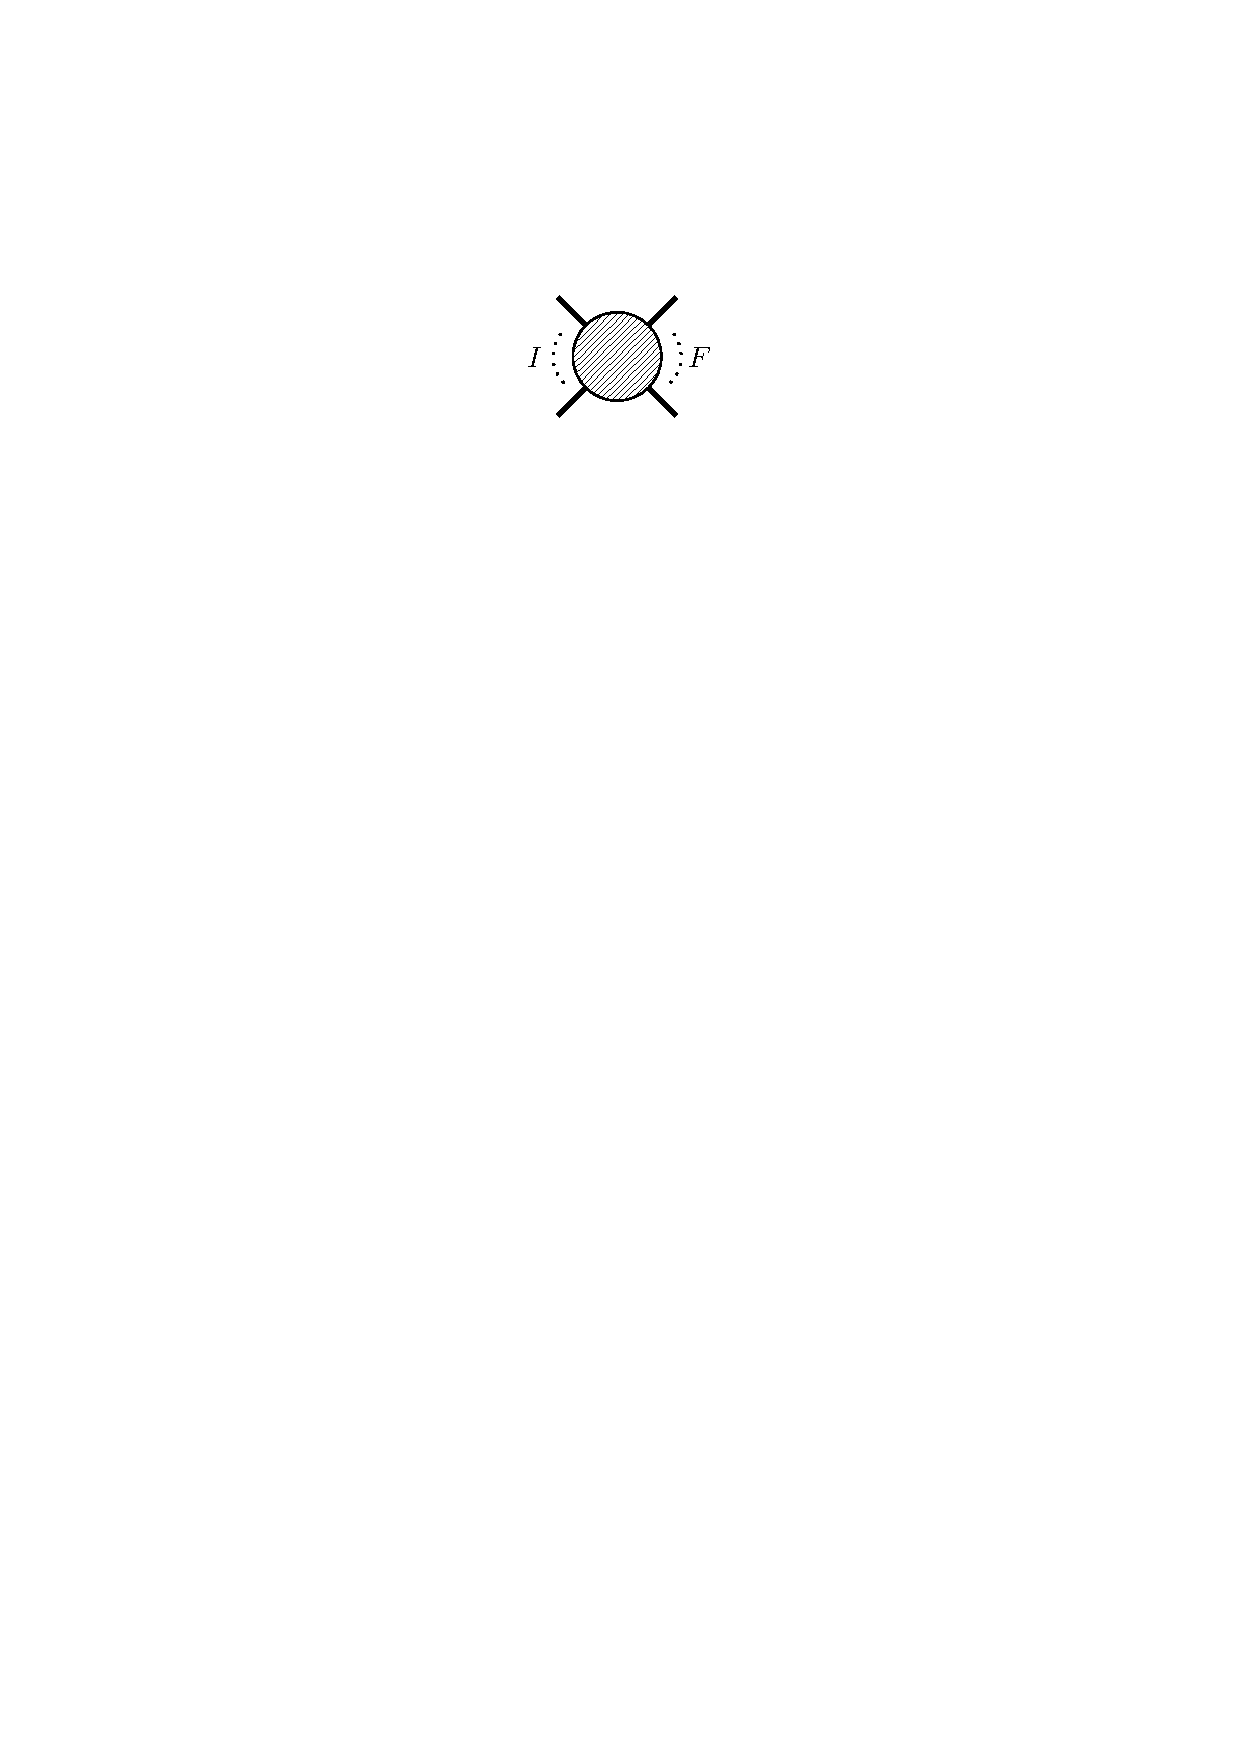
\includegraphics[width=1.5cm]{ch3_loopamps/figures/ampIFall.pdf}} \right) \\
  \end{aligned}
  \label{eq:amp-disc}
\end{align}
where the discontinuity is across the branch cut in the invariant $P^2$, \break ${\rm
Disc}_{P^2} \,A(\cdots,P^2,\cdots) =  A(\ldots,P^2+\i0,\ldots) -
A(\ldots,P^2-\i0,\ldots)$. This is referred to as the discontinuity in the $P^2$ channel.

We may now expanding the relation~\eqref{eq:unitarity-pictorial}
perturbatively, in a coupling $g$, which results in a set of extremely useful
equations for on-shell amplitudes. We can represent the perturbative expansion
of the amplitudes this pictorially by,
\begin{equation}
  \raisebox{-0.4cm}{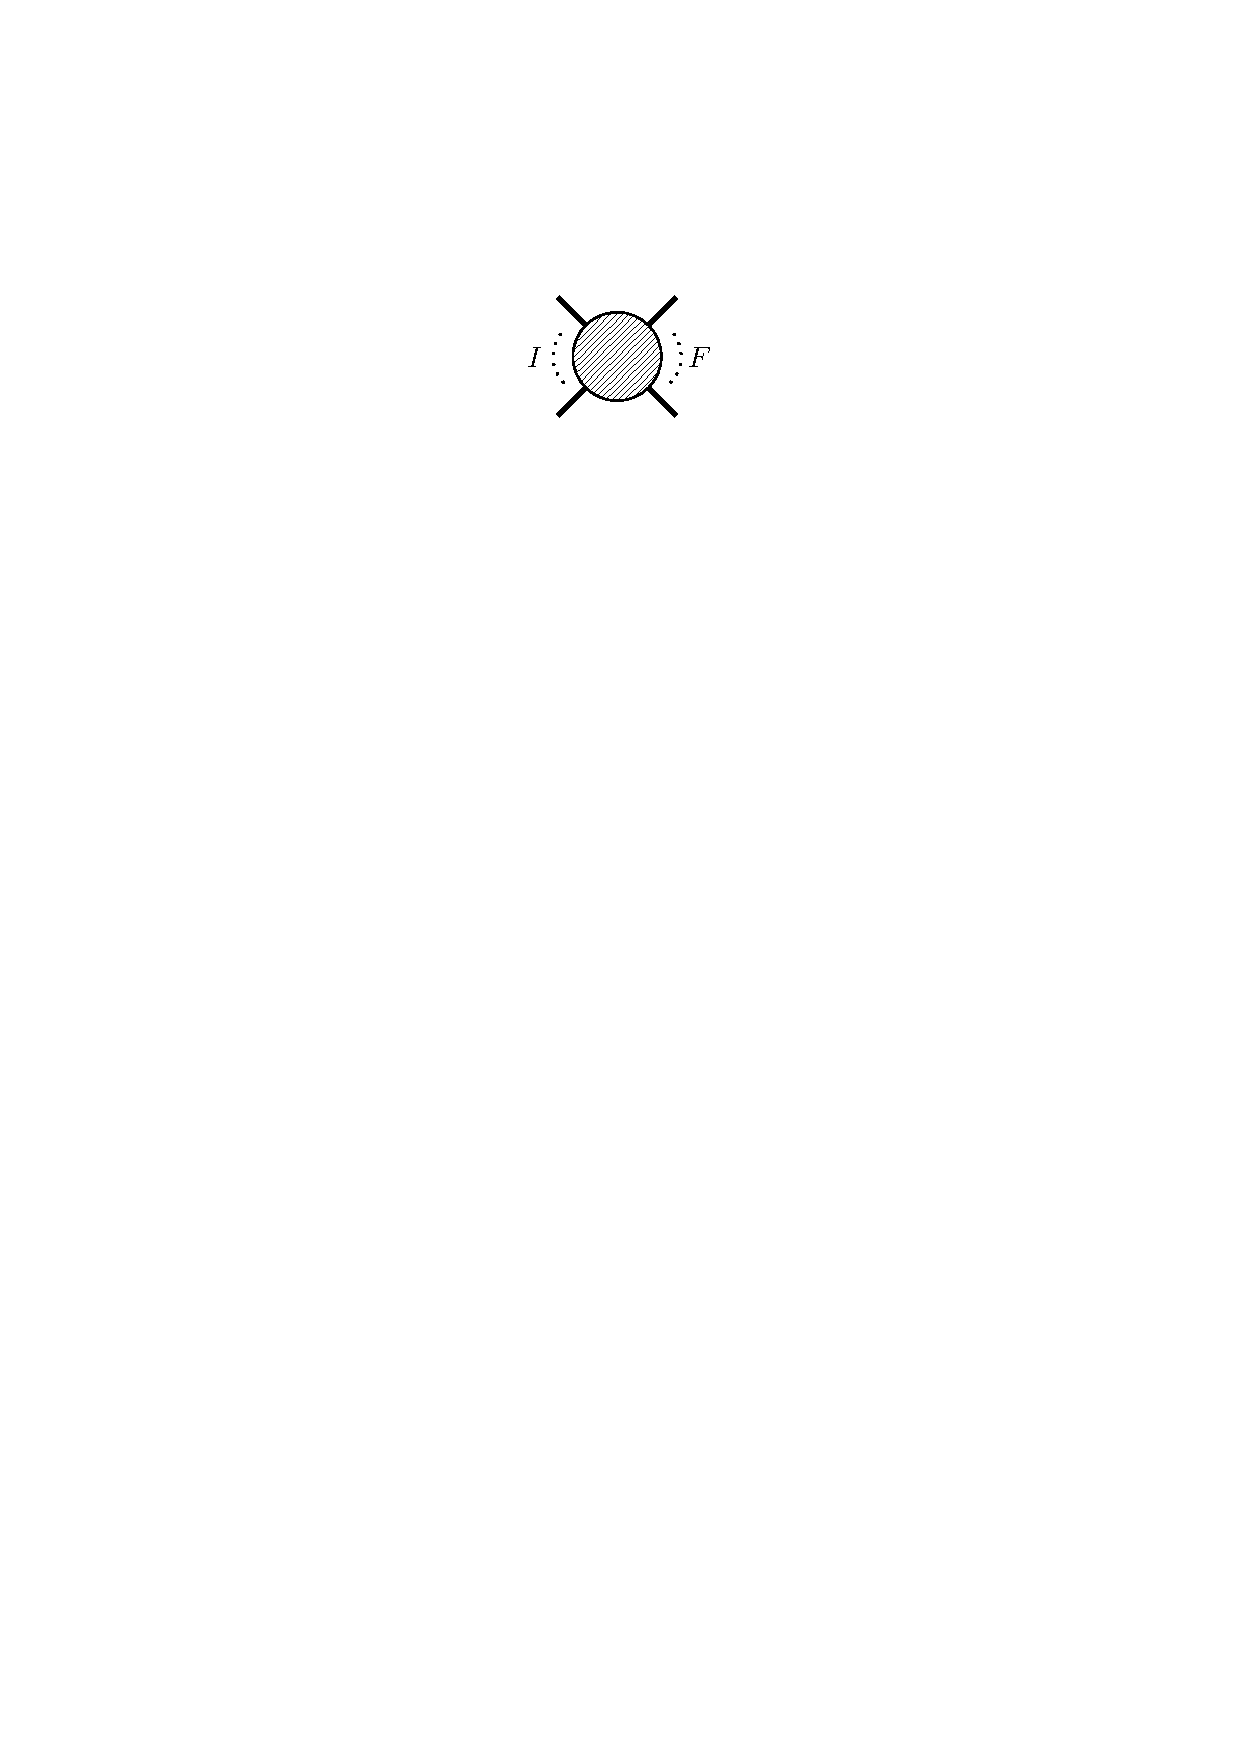
\includegraphics[width=1.5cm]{ch3_loopamps/figures/ampIFall.pdf}} = g^{\rm LO} \left(
  \raisebox{-0.4cm}{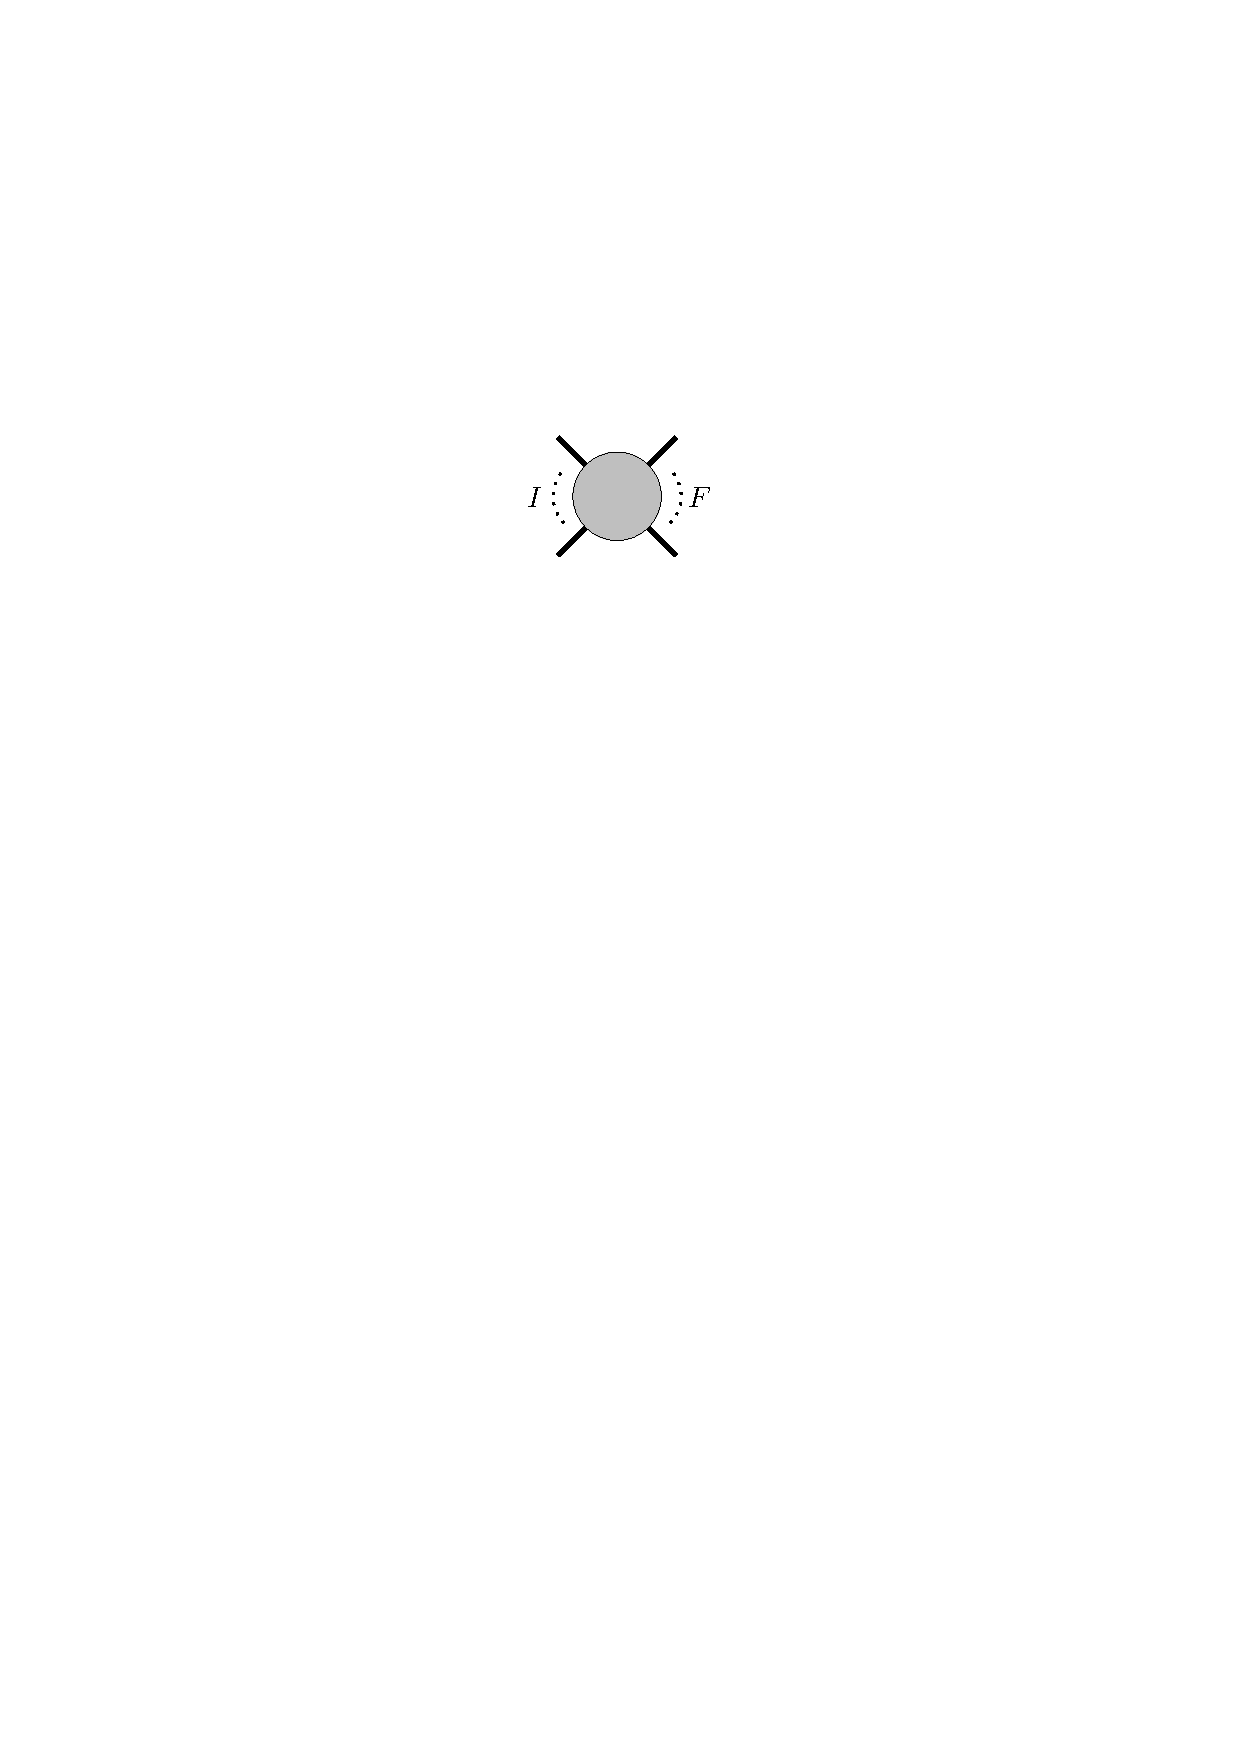
\includegraphics[width=1.5cm]{ch3_loopamps/figures/ampIF0.pdf}} +
  g^2 \raisebox{-0.4cm}{
\includegraphics[width=1.5cm]{ch3_loopamps/figures/ampIF1.pdf}} +
  g^4 \raisebox{-0.4cm}{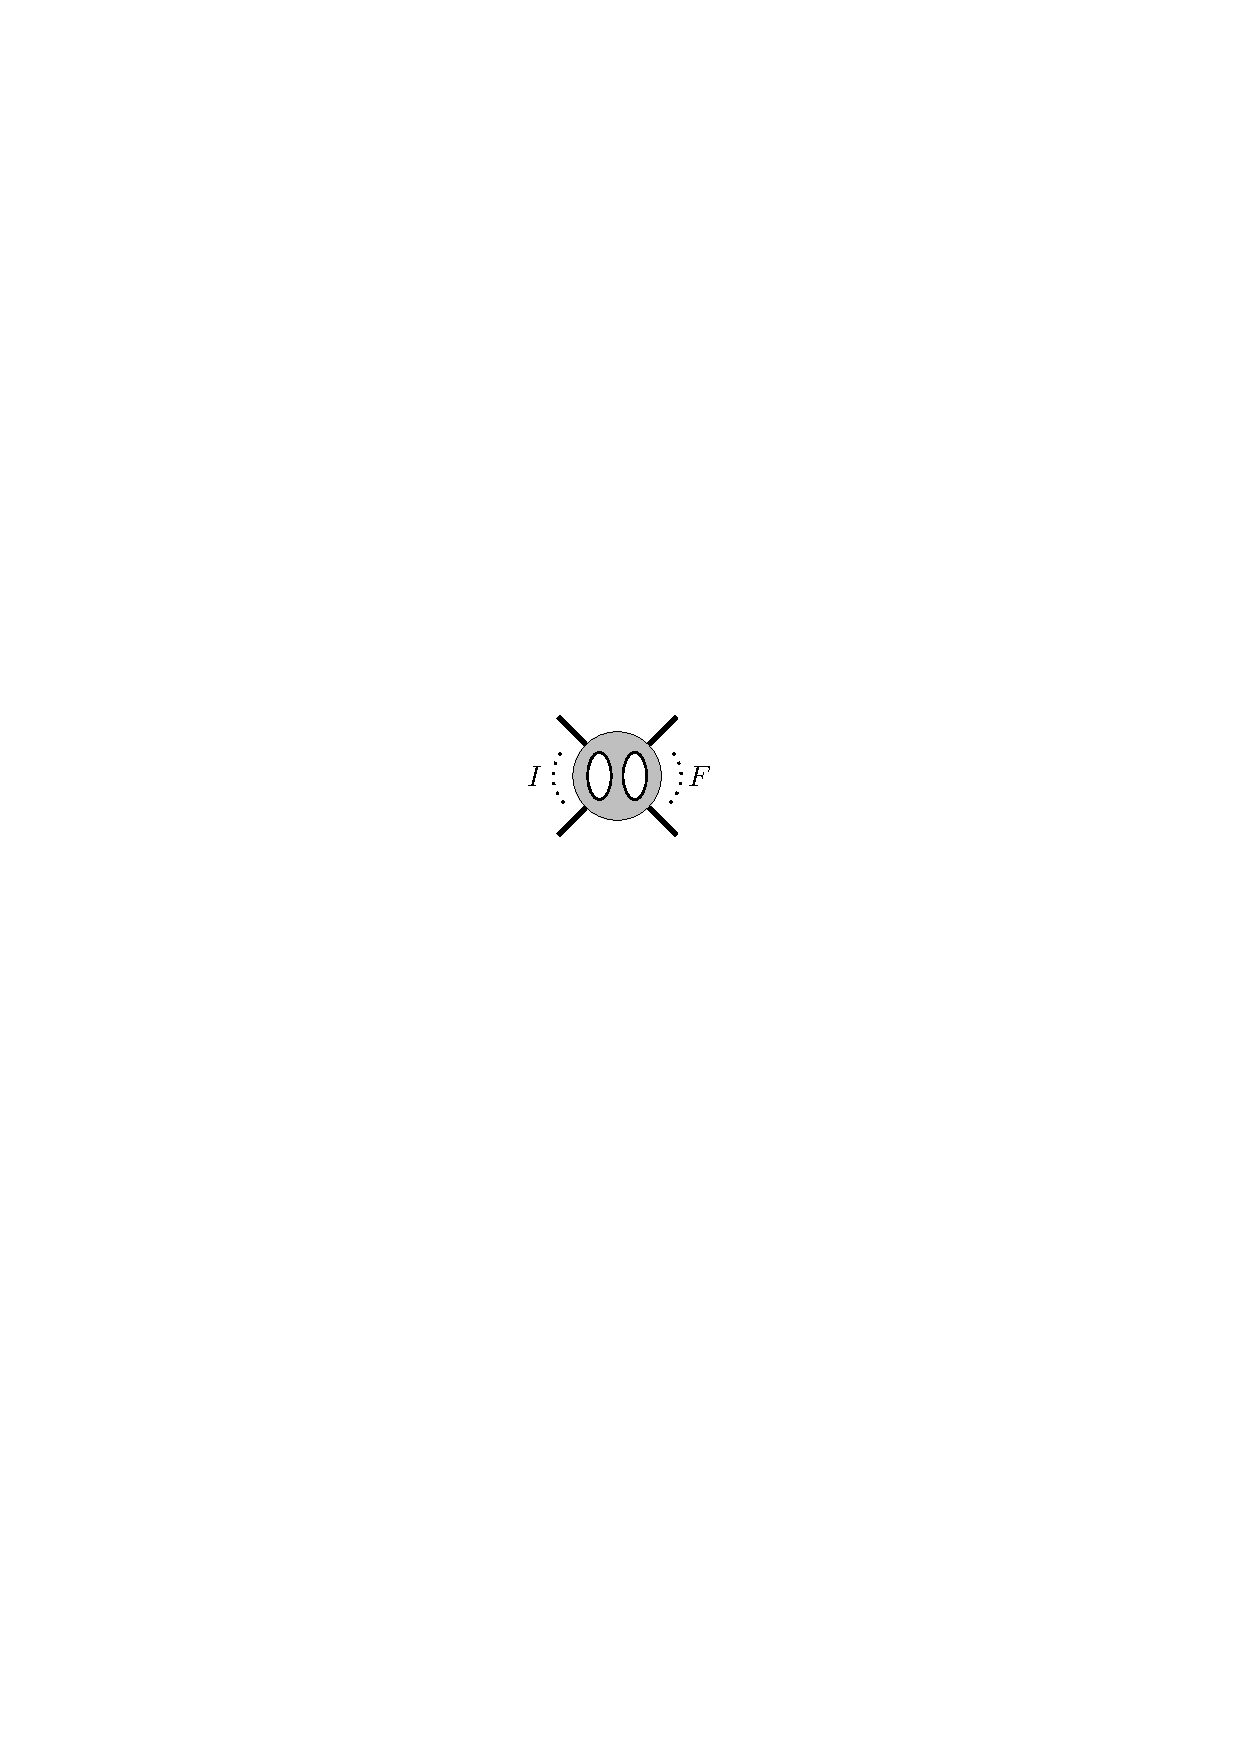
\includegraphics[width=1.5cm]{ch3_loopamps/figures/ampIF2.pdf}} + \ldots  \right) \,,
  \label{eq:pertexp-pictorial}
\end{equation}
where $g^{\rm LO}$ is the leading-order coupling (e.g.\ $g^{\rm LO} = g^{n-2}$
for a $n$-gluon amplitude in YM theory).  By substituting this expansion into
the unitarity relation~\eqref{eq:unitarity-pictorial} we find equations order
by order in the coupling $g$. Explicitly, up to third order we find
\begin{align}
  {\rm Disc}_{P^2}\left( \raisebox{-0.4cm}{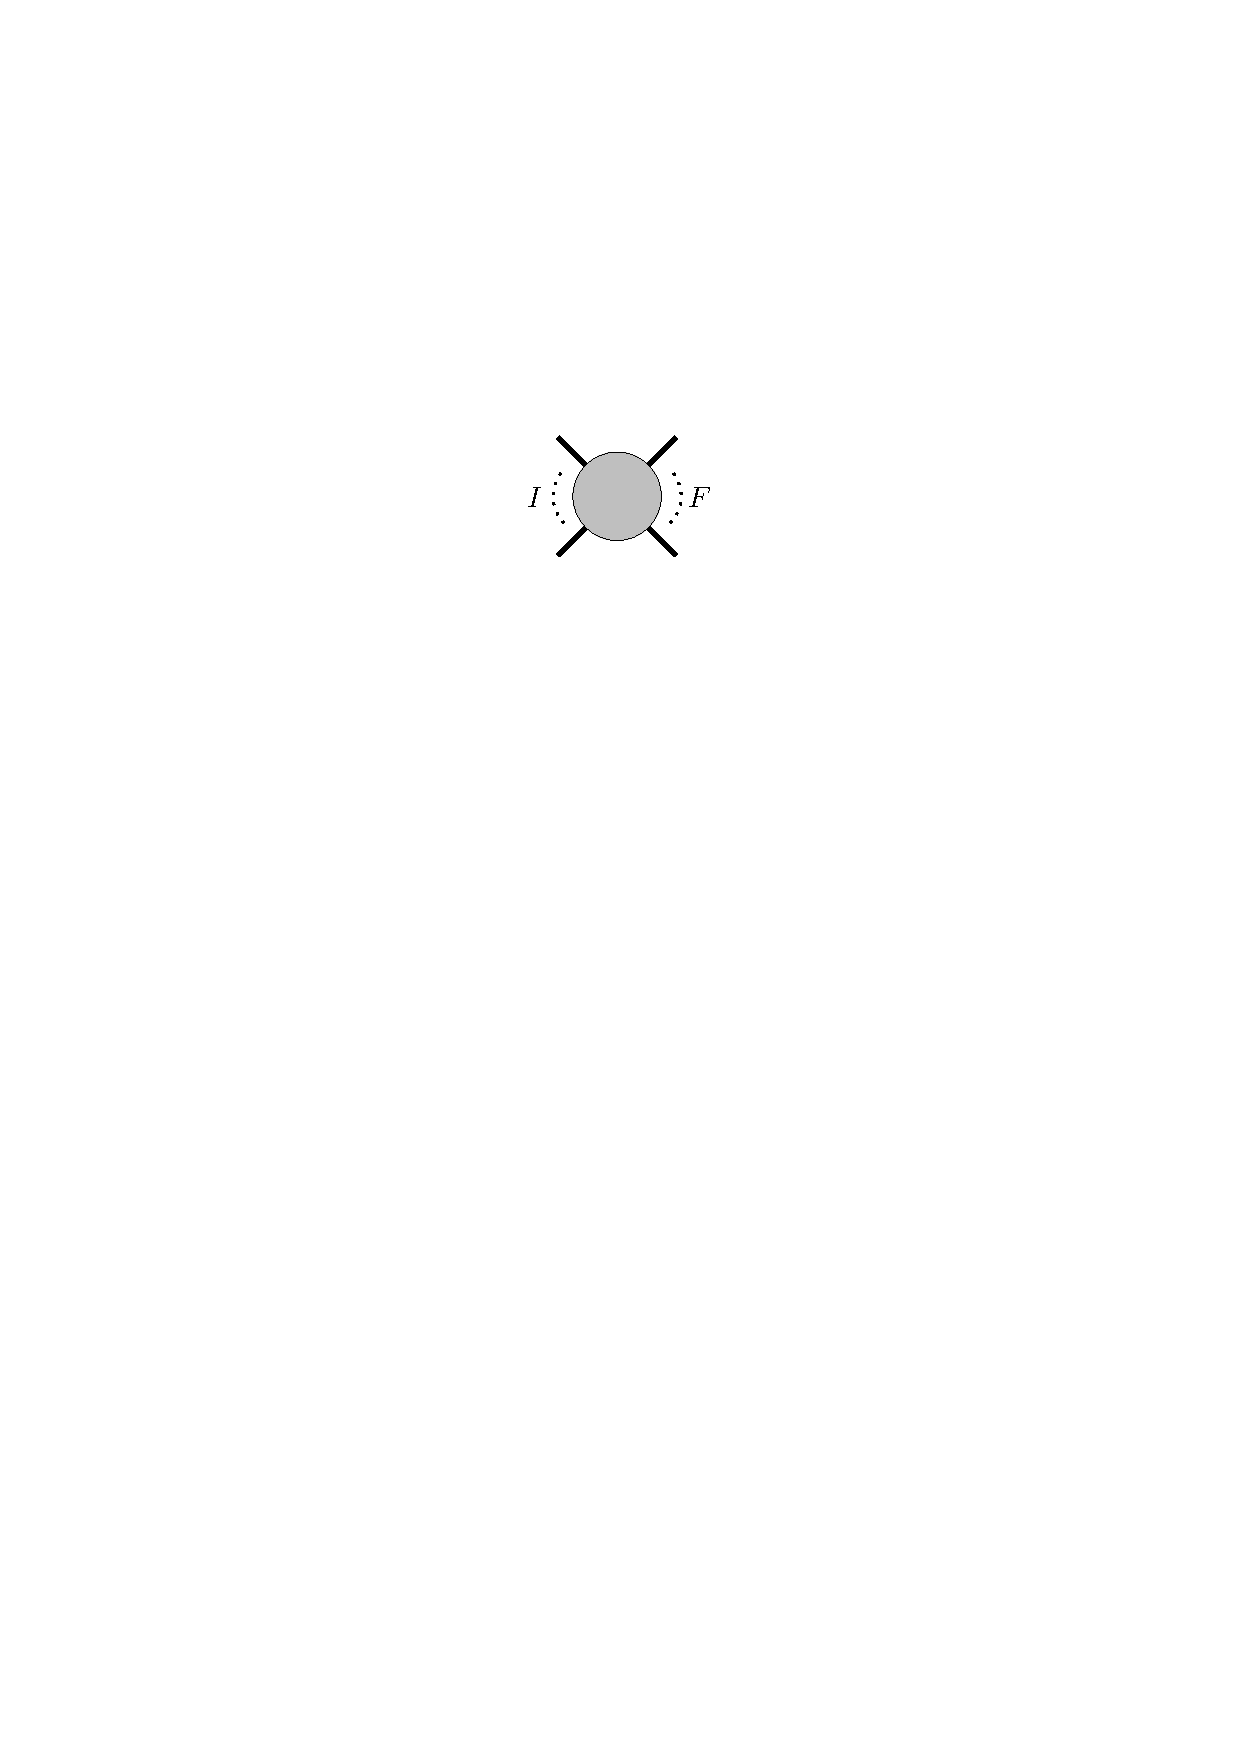
\includegraphics[width=1.5cm]{ch3_loopamps/figures/ampIF0.pdf}} \right) &= 0 \,, \\
  {\rm Disc}_{P^2}\left( \raisebox{-0.4cm}{
\includegraphics[width=1.5cm]{ch3_loopamps/figures/ampIF1.pdf}} \right) &=
         \int \d\Phi_2 \,\raisebox{-0.55cm}{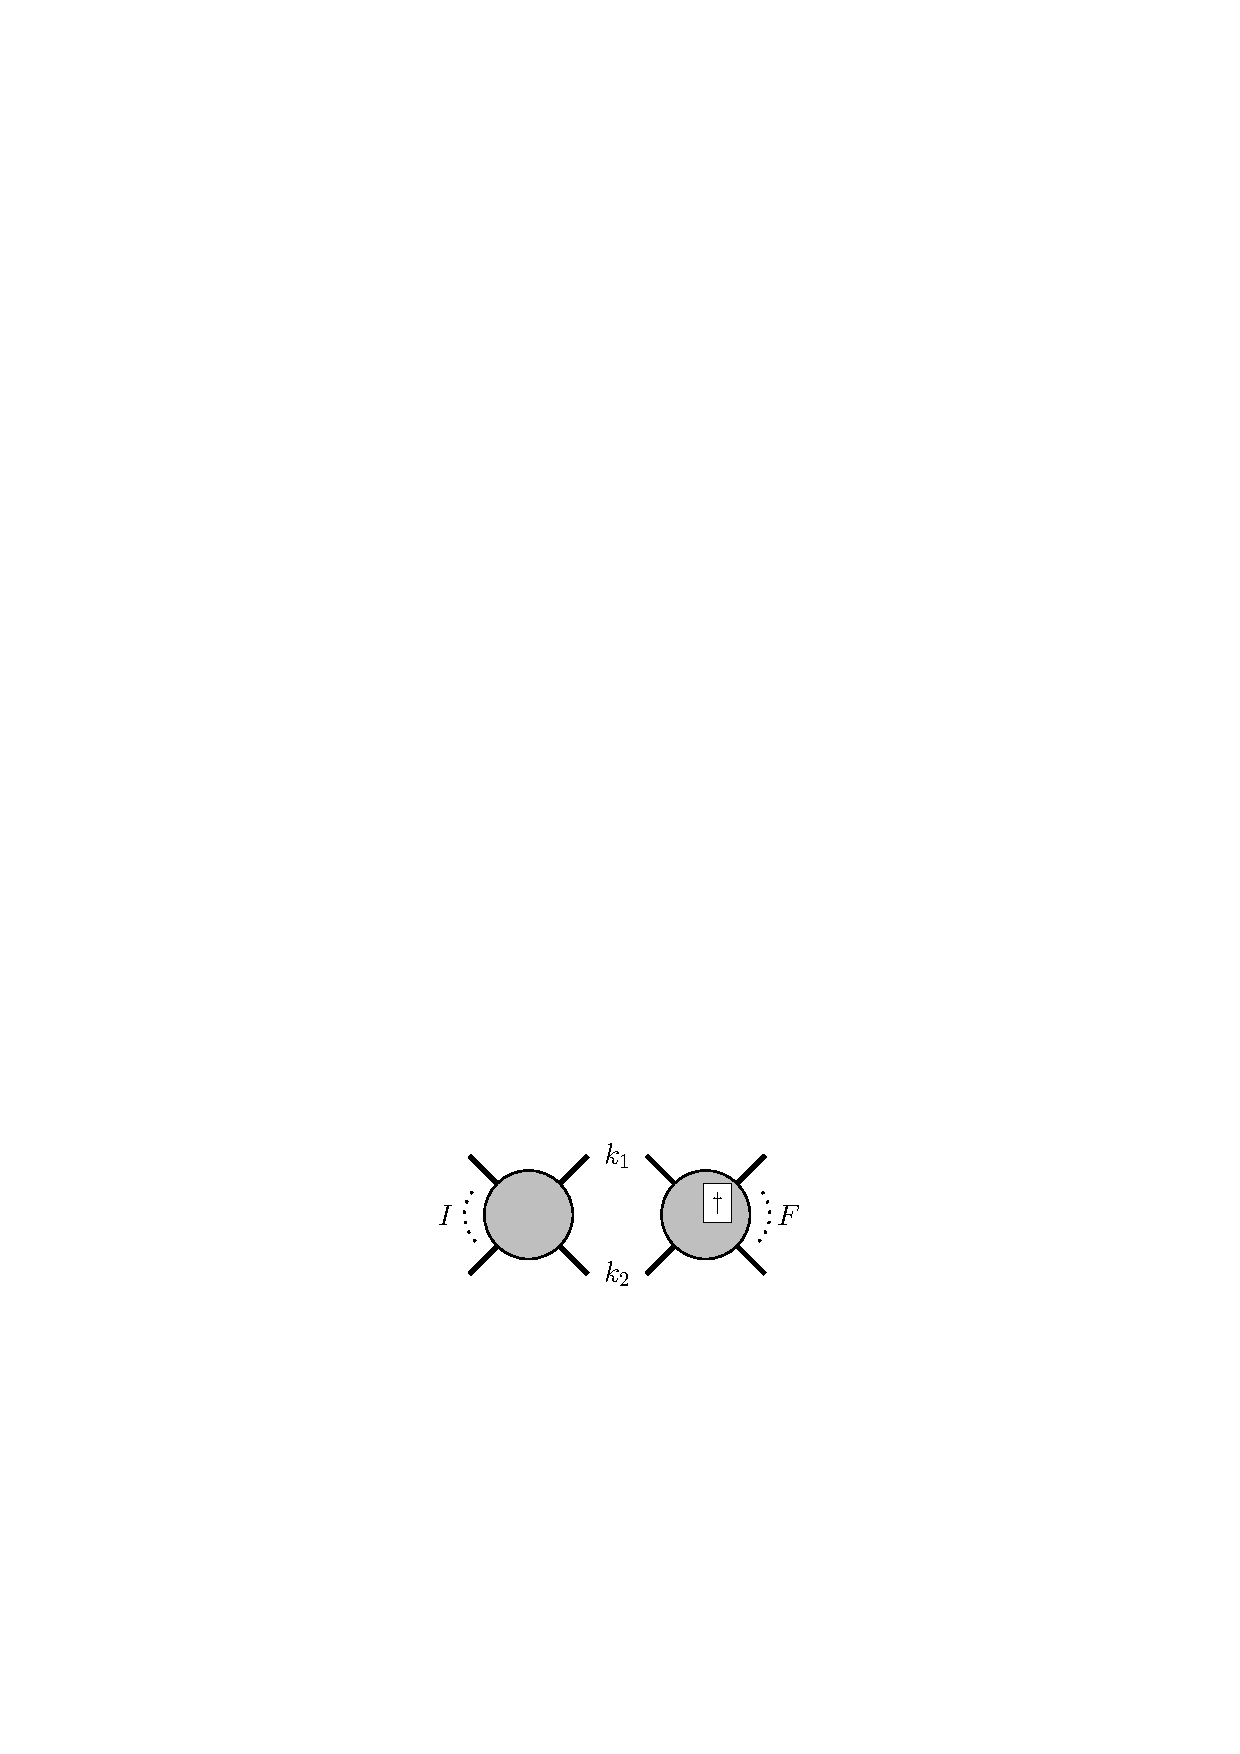
\includegraphics[width=3cm]{ch3_loopamps/figures/ampI00F2.pdf}} \,, \\
  {\rm Disc}_{P^2}\left( \raisebox{-0.4cm}{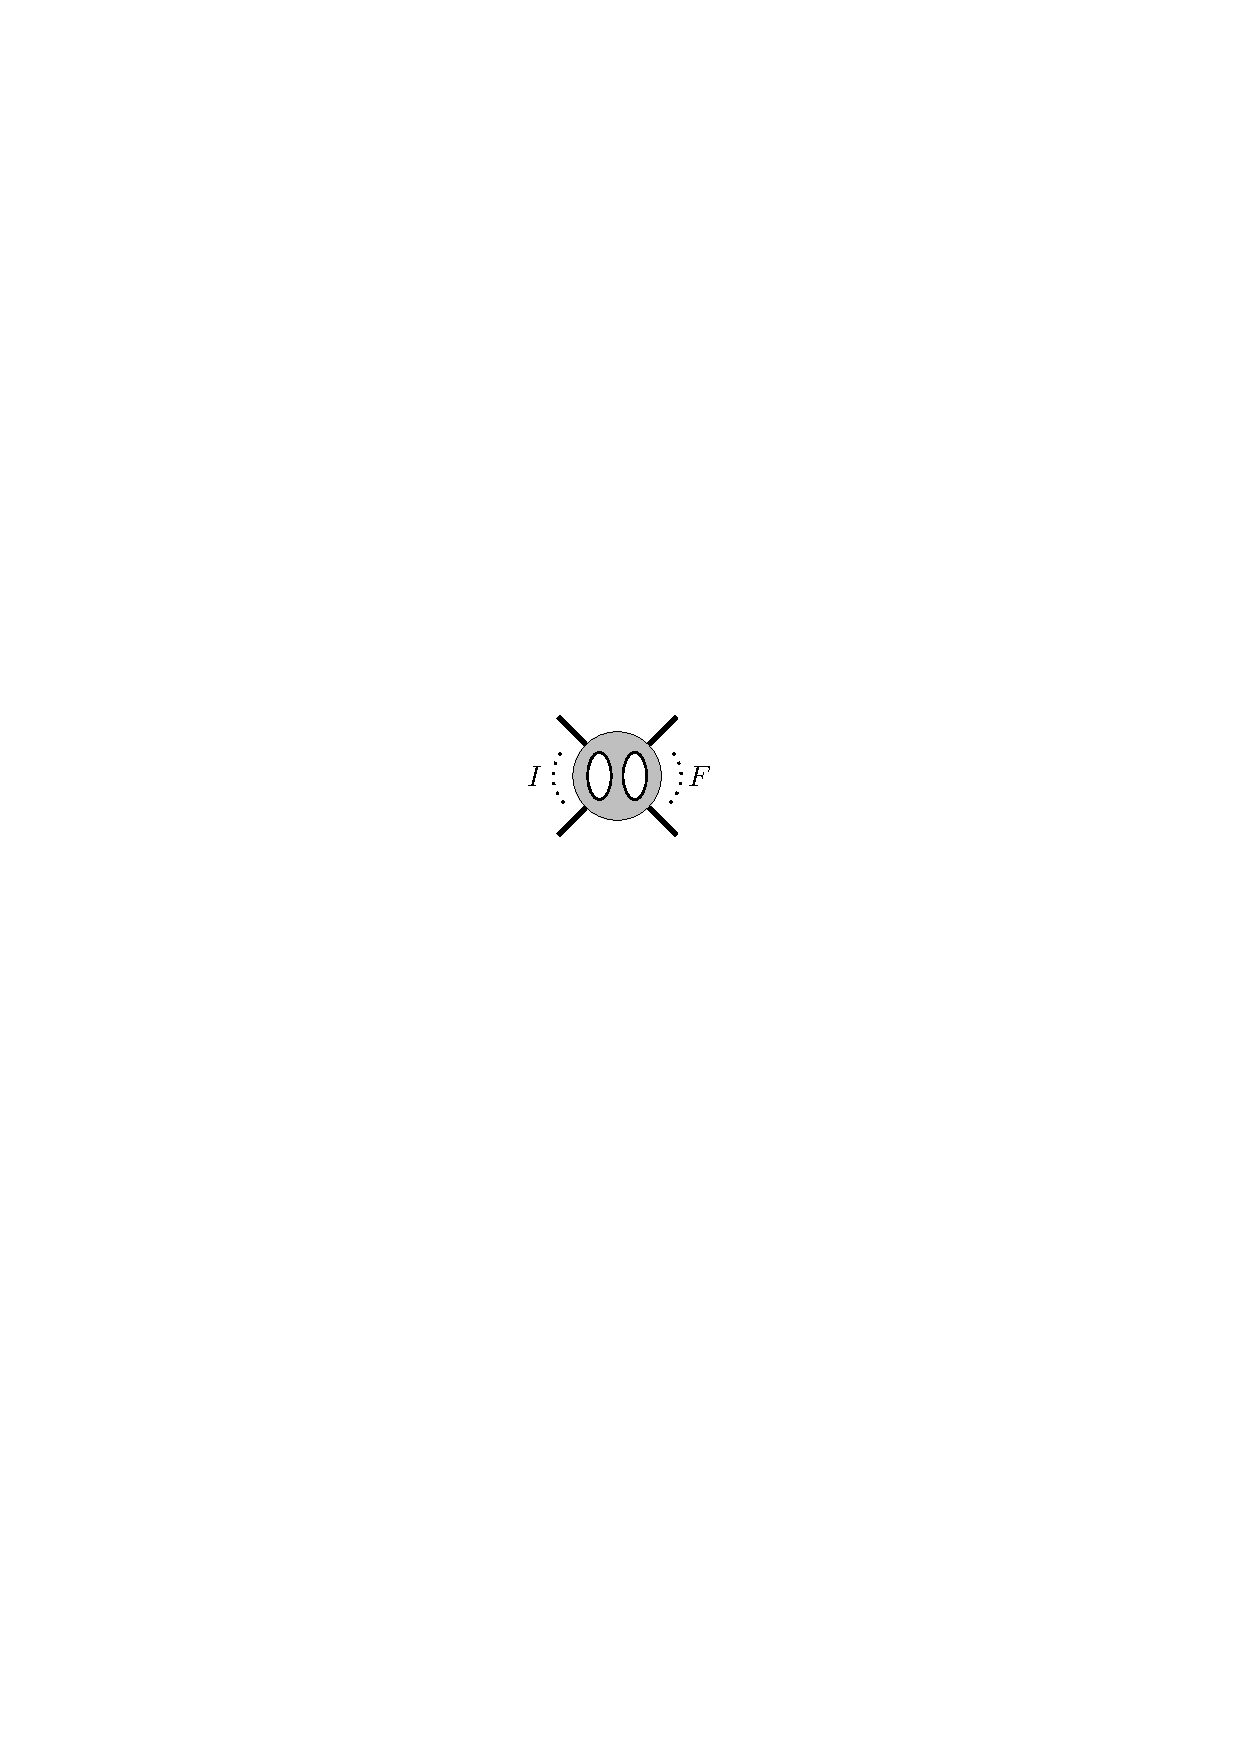
\includegraphics[width=1.5cm]{ch3_loopamps/figures/ampIF2.pdf}} \right) &=
  \int \d\Phi_2 \,\left( \raisebox{-0.55cm}{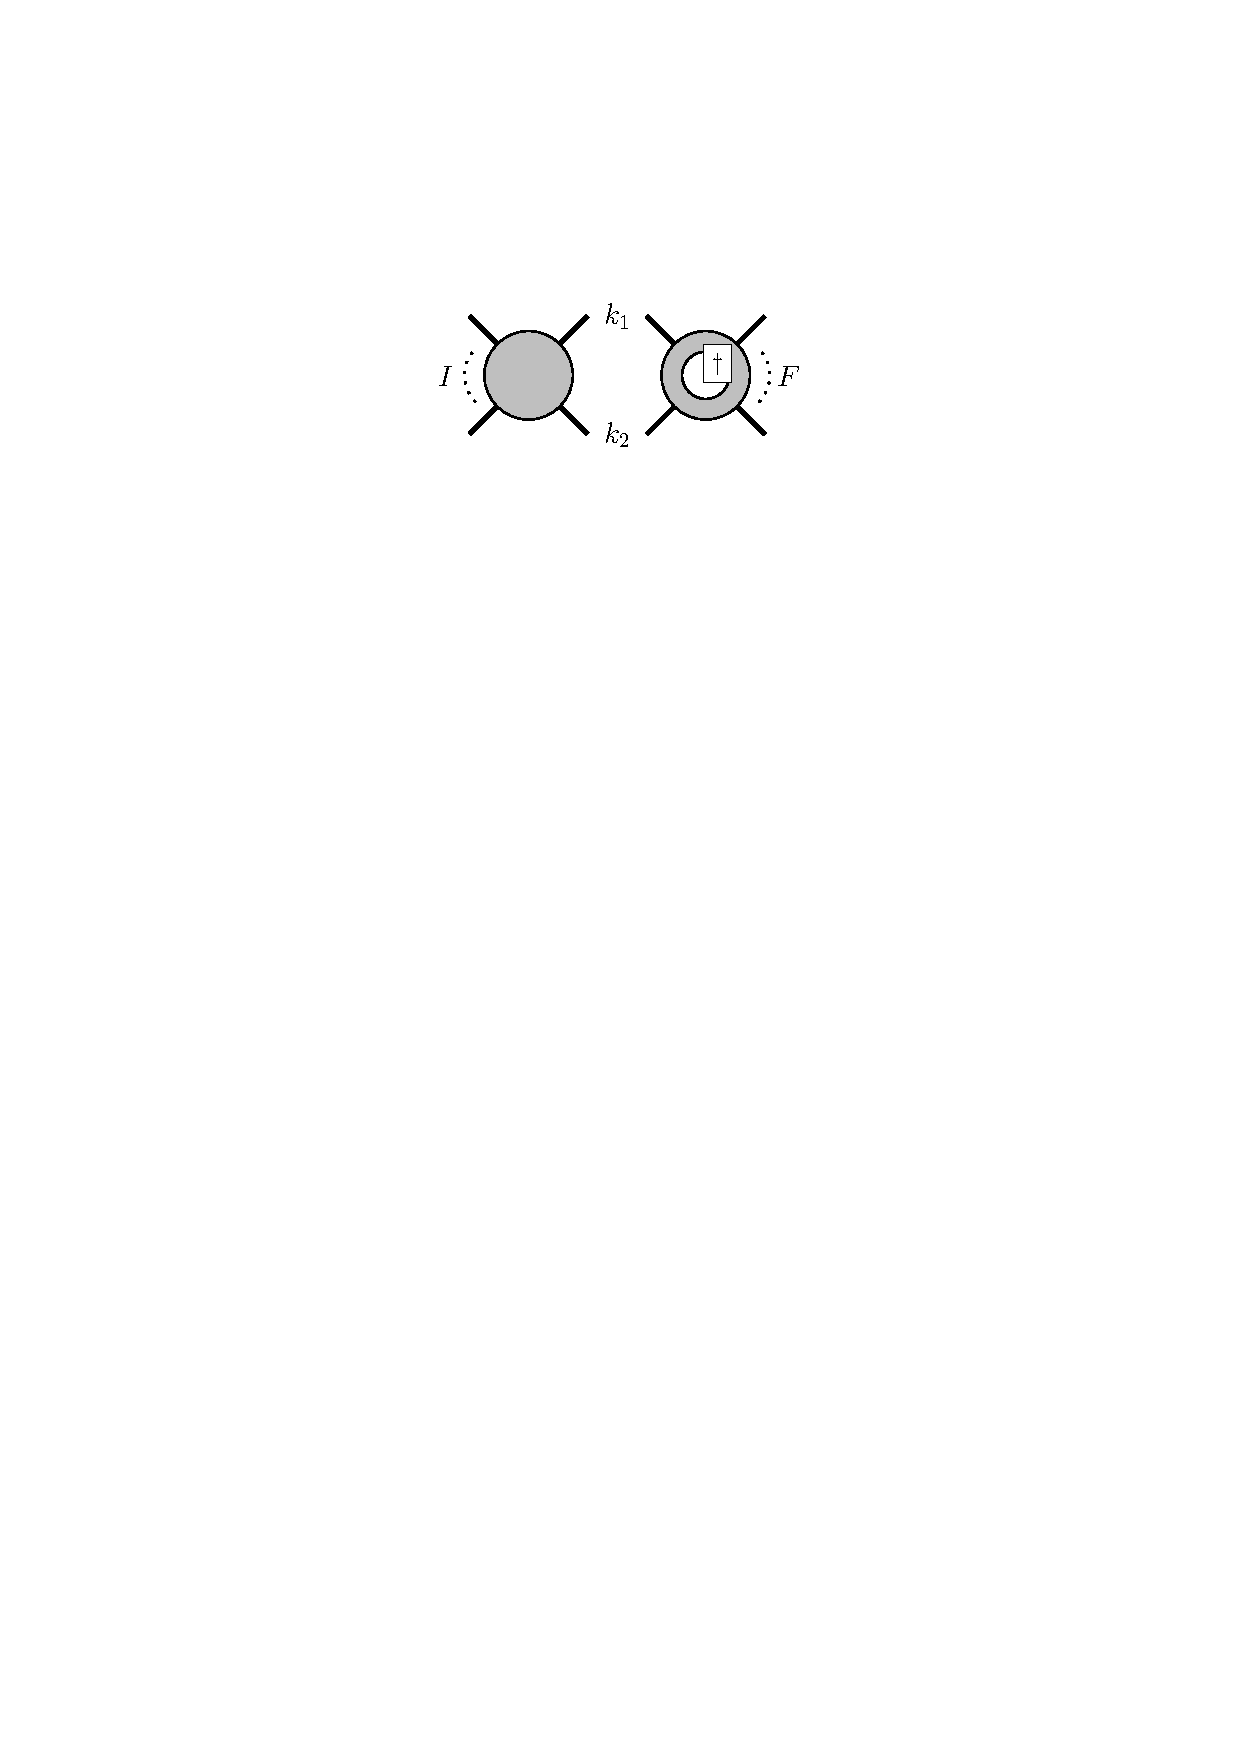
\includegraphics[width=3cm]{ch3_loopamps/figures/ampI01F2.pdf}}
                    + \raisebox{-0.55cm}{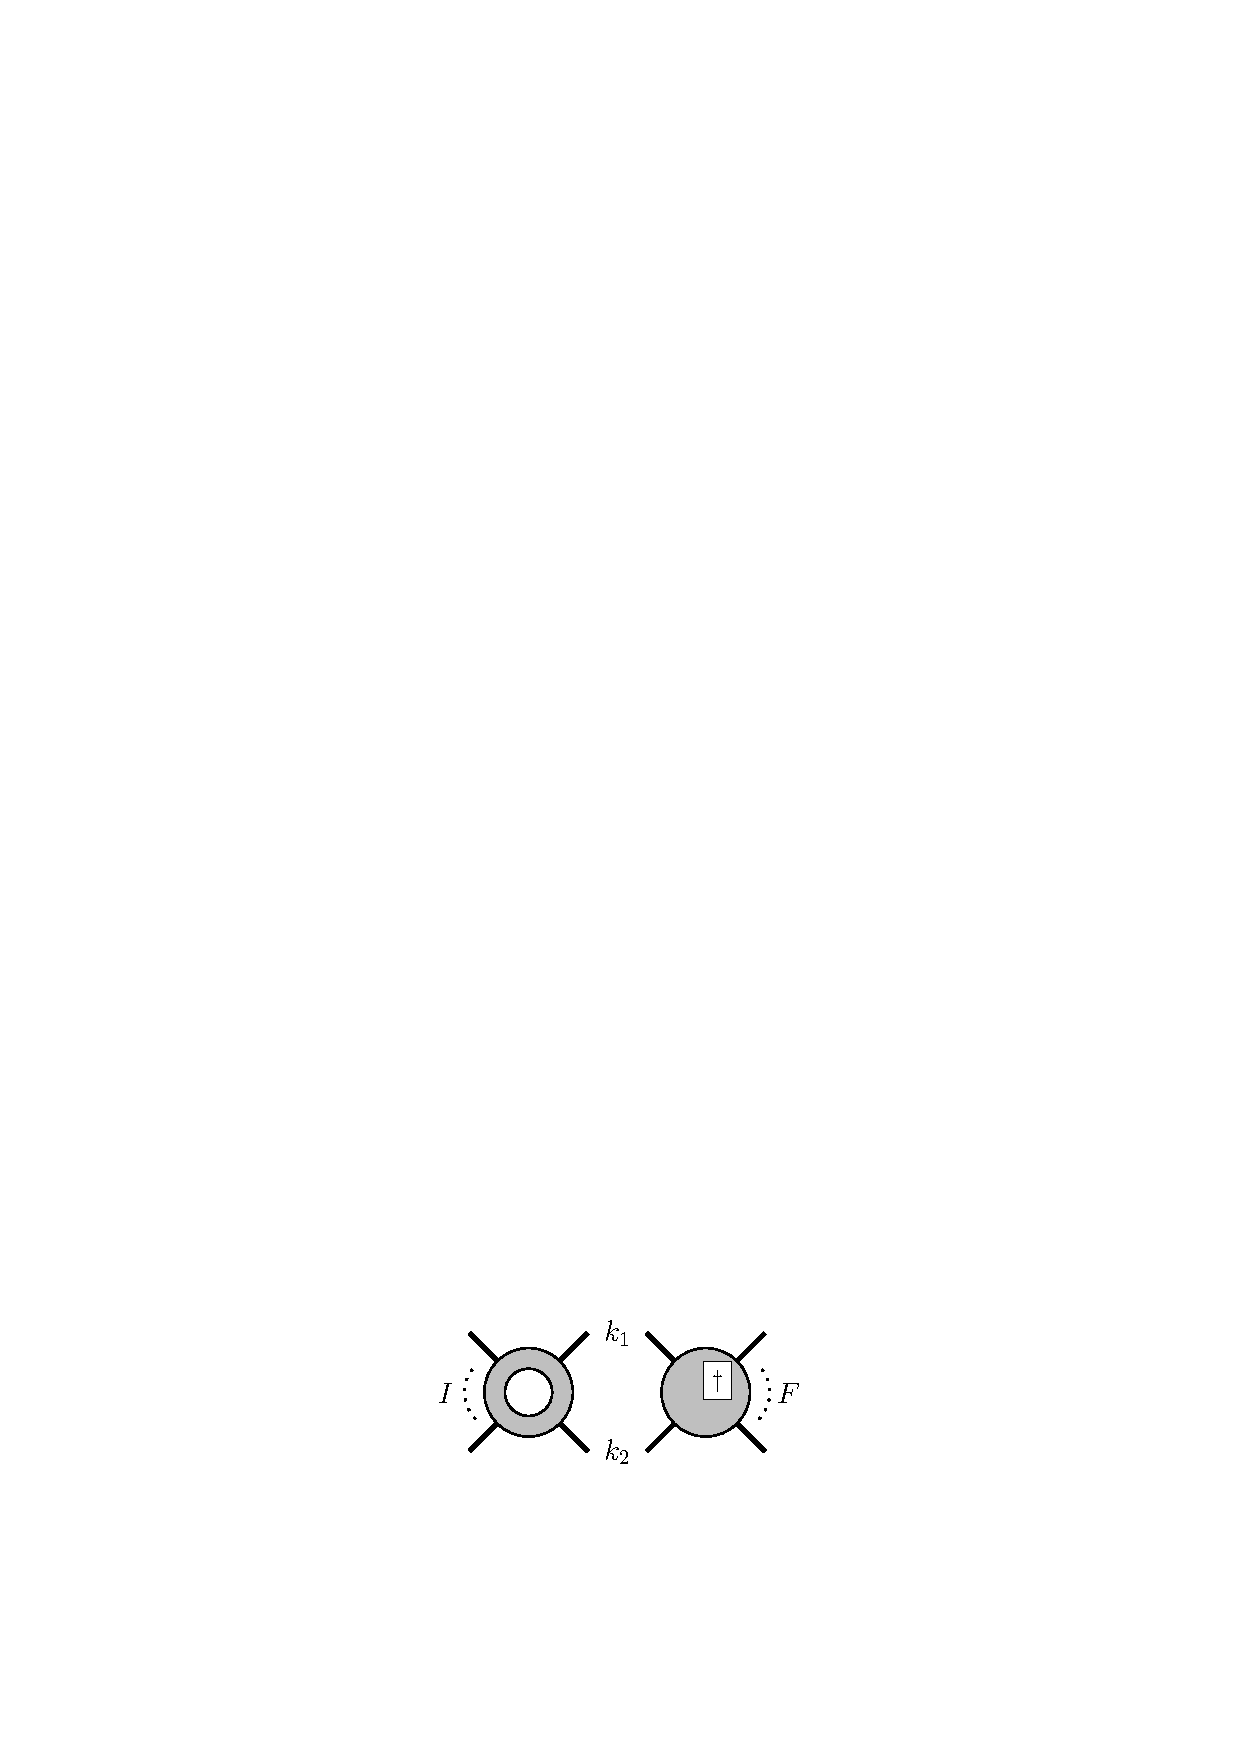
\includegraphics[width=3cm]{ch3_loopamps/figures/ampI10F2.pdf}} \right)\nonumber\\& \phantom{= {}}
       + \int \d\Phi_3 \,\raisebox{-0.55cm}{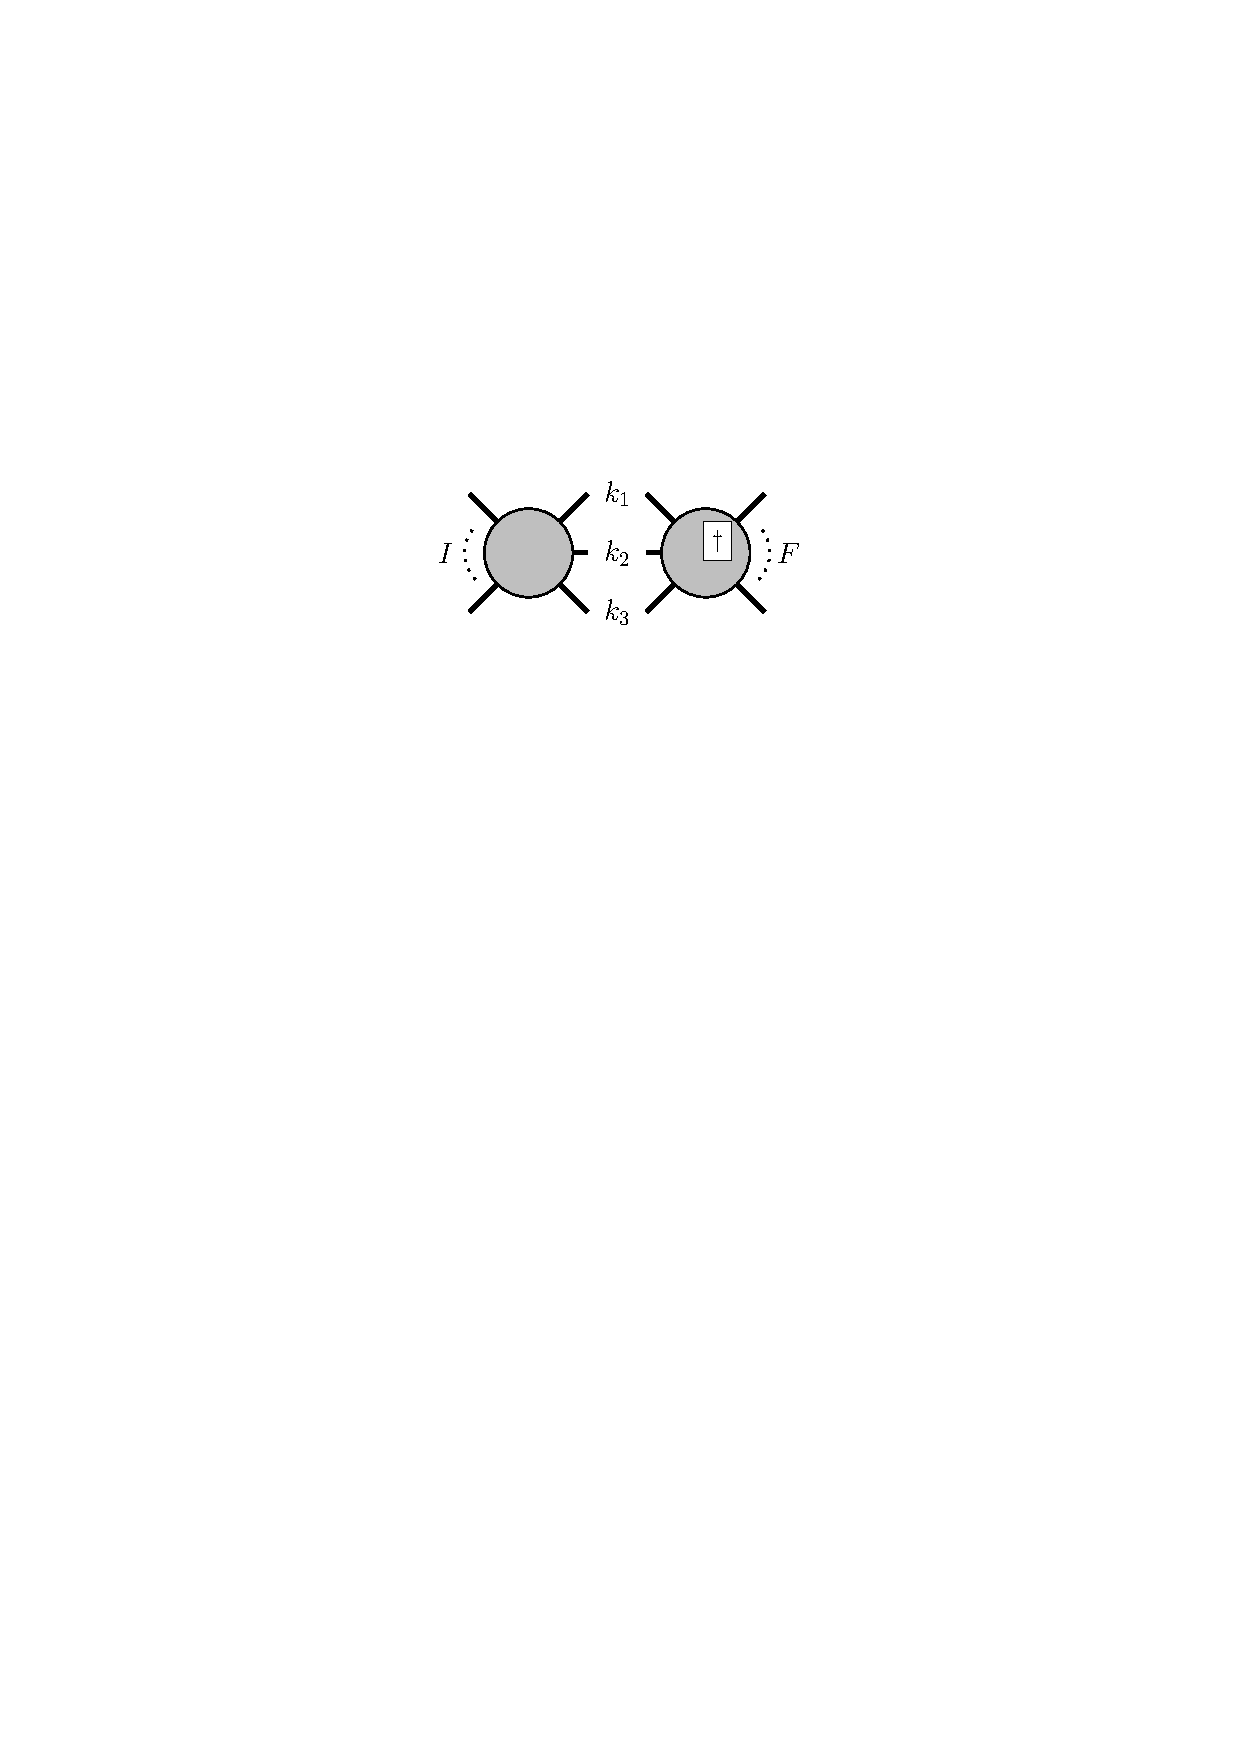
\includegraphics[width=3cm]{ch3_loopamps/figures/ampI00F3.pdf}} \,.
\end{align}
The first of these equations confirms that rational tree-level amplitudes do
not contain branch cuts. At one-loop order we find that the product of two
\textit{on-shell} tree-level amplitudes is directly related to the
discontinuity in the channel $P^2$ of the one-loop amplitude.

Re-using the on-shell tree-level amplitudes we have found in chapters~\ref{ch:intro} and~\ref{ch:trees} inside the factorised loop integrand is an extremely efficient way of
computing the discontinuity of a loop amplitude. It avoids some of the large
intermediate algebraic steps that would be found following the expansion of the
loop amplitude into Feynman diagrams. The act of putting an internal propagator
on-shell, as we have done through the insertion of a complete set of states, is
referred to a the \emph{cut} of a loop amplitude.

However, we must still find a way to upgrade the discontinuity of the amplitude to the
full amplitude. One method to do this is to perform a dispersion integral. To
express this concretely, let us specify that the amplitude depends on $r$
invariants $s_1 = P_1^2,\ldots,s_r = P_r^2$. Then, we have that 
\begin{equation}
  A^{(1)}(s_1,\cdots,s_r) = \sum_{i=1}^r \int \frac{\d s'_i}{s_i'-s_i} \, {\rm Disc}_{s_i} \,A^{(1)}.
  \label{eq:dispersion}
\end{equation}
This story has been known for a long time and traces back to the work of
Cutkosky~\cite{ch3_Cutkosky:1960sp} and the days of the analytic $S$-matrix~\cite{ch3_Eden:1966dnq}.
The modern unitarity method (Bern, Dixon, Dunbar, Kosower~\cite{ch3_Bern:1994zx})
transformed the approach into a powerful computational tool by the cut
constraints with knowledge of a \textit{basis} of loop integrals, and the
spinor-helicity method for the compact representation of on-shell tree
amplitudes. Rather than computing the dispersion relation, one uses the
unitarity cut constraints to project out information about the rational
integral coefficients from a representation of the amplitudes such as the one
shown in \eqn{eq:loopamp-general}. It is this procedure that we refer to as
\textit{cut construction} of a scattering amplitude.

The on-shell phase space $\d\Phi_n$ contains Dirac $\delta$ functions which
ensure the intermediate particles are on-shell. We recall in fact that
\eqn{eq:phase_space} can be rewritten in a manifestly Lorentz-invariant form as
\begin{align}
\d\Phi_n(P, \{k\}_n) = (2\pi)^4 \delta^{(4)}\left( P-\sum_n k_n \right) \prod_{i=1}^n \frac{\d^4 k_i}{(2\pi)^4 } (2\pi) \delta^{(+)}\bigl(k_i^2-m_i^2 \bigr) \,,
\end{align} 
where
\begin{align}
 \delta^{(+)}\bigl(k_i^2-m_i^2 \bigr) \coloneqq  \delta \bigl(k_i^2-m_i^2 \bigr) \, \Theta\bigl(k_i^0\bigr)\,,
\end{align}
with the Heaviside step function $\Theta$ ensuring the positivity of the energy.

Since it will become a fundamental part of our amplitude analysis, it is useful to introduce some
notation for the action of imposing these on-shell constraints on internal
particles of a loop diagram. The operation of computing the discontinuity
across a two-particle factorisation or \emph{cut} will be represented as $\mathcal{C}_{L|R}$, where
the indices $L$ and $R$ will be the list of external particles entering the left and right side of the cut respectively,
\begin{align}
  & \mathcal{C}_{i_1\ldots i_m|i_{m+1}\ldots i_n}\left( A_n^{(1),[D]} \right) \coloneqq {\rm Disc}_{s_{i_1\ldots i_m}}\left( A_n^{(1),[D]} \right)
     \nonumber\\
    &= \int \d\Phi_2 \sum_{h_i=\pm}
       \i A_{m+1}^{(0)}\bigl(-l_1^{-h_1}, i_1,\ldots,i_m, l_2^{h_2} \bigr)
    \, \i A_{n-m+2}^{(0)}\bigl(-l_2^{-h_2}, i_{m+1},\ldots,i_n, l_1^{h_1} \bigr) \,,
  \label{eq:Cnotationdef}
\end{align}
where
\begin{align} 
\label{eq:onshellPSmeasure}
\begin{aligned}
  \d\Phi_2 & =
  \frac{\d^4 l_1}{(2\pi)^4}
  \frac{\d^4 l_2}{(2\pi)^4}
     (2\pi)^4 \delta^{(4)}(l_1-l_2-p_{i_1\ldots i_m}) \\
     & \phantom{= {}} \times  (2\pi) \delta^{(+)}(l_1^2-m_1^2) \, (2\pi) \delta^{(+)}(l_2^2-m_2^2) \,.
\end{aligned}
\end{align}
The $\delta$ functions ensure momentum conservation, and that the internal
momenta $l_1$ and $l_2$ are at their on-shell values $m_1$ and $m_2$.
Notice that two factors of $\i$ appear in the factorisation into tree
amplitudes. This appears for exactly the same reason as it did in BCFW
recursion, where each factorised on-shell gluon propagator contributed a factor of
$\i$ (see below \eqn{eq:multiparticlepole}). For fermion propagators this factor would change as discussed in section~\ref{sec:2.1} and exercise~\ref{Ex:3.1}.  

We will also use the operation $\mathcal{C}_{L|R}$ to act on the integrand of the amplitude,
and therefore only represent the product of tree-level amplitudes,
\begin{align}
\begin{aligned}
   &\mathcal{C}_{i_1\ldots i_m|i_{m+1}\ldots i_n}\left( I_n^{(1),[D]} \right)
    = \\
   & \sum_{h_i=\pm} \i A_{m+2}^{(0)} \bigl(-l_1^{-h_1}, i_1,\ldots,i_m, l_2^{h_2} \bigr) \, \i A_{n-m+2}^{(0)}\bigl(-l_2^{-h_2}, i_{m+1},\ldots,i_n, l_1^{h_1} \bigr) \,,
 \end{aligned}
  \label{eq:Cnotationdef}
\end{align}
where the on-shell conditions for $l_1$, $l_2$ are understood to be imposed.

\begin{example}{Example: The $s_{12}$-channel cut of the $gg\to gg$ MHV scattering amplitude}

  Let us consider the leading-colour\footnote{This is the coefficient of the single-trace term in the colour ordered one-loop amplitude given in \eqn{leading-colour-one-loop}, denoted there as $A^{(1)}_{n;1}.$} four-gluon MHV amplitude in
pure Yang-Mills theory, $A^{(1)}(1^-,2^-,3^+,4^+)$. We begin with the familiar
Parke-Taylor formula~\eqref{ParkeTaylor1} for the tree amplitudes (this time setting the coupling to 1),
\begin{equation}
  A^{(0)}(1^-,2^-,3^+,4^+) = \frac{\i \spA12^3}{\spA23\spA34\spA41} \,.
  \label{eq:4gtree}
\end{equation}
Note that by using the four-dimensional tree-level amplitudes inside the cut we are only resolving the first term in the expansion of the integral coefficient expressed in \eqn{eq:coeffexp}.
The $s_{12}$-channel is associated with the invariant $s_{12} = (p_1+p_2)^2$, and the discontinuity
is obtained from the following product of two tree amplitudes summed over all possible
helicity states,
\begin{equation}
  \mathcal{C}_{12|34}\left( I_4^{(1)}(1^-,2^-,3^+,4^+) \right) = \sum_{h_i=\pm} \i A^{(0)}(-l_1^{-h_1},1^-,2^-,l_2^{h_2}) \, \i A^{(0)}(-l_2^{-h_2},3^+,4^+,l_1^{h_1}) \,,
  \label{eq:4gschannelintegrand}
\end{equation}
where, as imposed by the Lorentz invariant phase-space measure $\d\Phi_2$,
$l_2=l_1-p_{12}$ and $l_i^2=0$. Since all tree amplitudes with all-like
helicities or those with a single positive (or negative) helicity vanish, only
a single term contributes to the cut. In order to keep the notation as compact
as possible, we will use $\mathcal{C}_{12|34}$ to refer to
$\mathcal{C}_{12|34}\bigl(I_4^{(1)}(1^-,2^-,3^+,4^+)\bigr)$ 
for the remainder of this section. Replacing the tree-level amplitudes with their spinor-bracket forms leads to
\begin{align}
  \mathcal{C}_{12|34} & = \i \, A^{(0)}(-l_1^{+},1^-,2^-,l_2^{+}) \, \i \, A^{(0)}(-l_2^{-},3^+,4^+,l_1^{-}) \nonumber\\
  &= \frac{\spA12^3}{\spA2{l_2}\spA{l_2}{(-l_1)}\spA{(-l_1)}1} \frac{\spA{l_1}{(-l_2)}^3}{\spA{(-l_2)}3\spA34\spA4{l_1}} \nonumber\\
  \label{eq:C12|34YM}
  &= \frac{\spA12^3}{\spA2{l_2}\spA{l_2}{l_1}\spA{l_1}1} \frac{\spA{l_1}{l_2}^3}{\spA{l_2}3\spA34\spA4{l_1}} \,.
\end{align}
Above we have used the phase convention~\eqref{negpspin} for the spinors of the loop momenta, namely $|(-l_i)\ran = \i |l_i\ran$.
We can now apply some spinor identities to recast the integrand into a form that
can be identified with one-loop integral topologies. For example,
\begin{equation}
  \spA{l_1}1 = \frac{2 \, l_1\cdot p_1}{\spB1{l_1}} = -\frac{(l_1-p_1)^2}{\spB1{l_1}} \,.
\end{equation}
Hence we find
\begin{align}
  \mathcal{C}_{12|34} &= \frac{\spA12^3}{\spA34} \frac{\spA{l_1}{l_2}^2 \spB2{l_2}\spB{l_1}1\spB{l_2}3\spB4{l_1}}{(l_2+p_2)^2 (l_1-p_1)^2 (l_2-p_3)^2(l_1+p_4)^2} \nonumber\\
  &= \frac{\spA12^3}{\spA34} \frac{\spBB{1}{l_1 l_2}{2}\spBB{3}{l_2 l_1}{4}}{(l_2+p_2)^2 (l_1-p_1)^2 (l_2-p_3)^2(l_1+p_4)^2} \,.
\end{align}
The numerator can also be reduced using the on-shell kinematics,
\begin{equation}
  \spBB{1}{l_1 l_2}{2} = \spBB{1}{l_1 (l_1-p_{12})}{2} = -\spAB{1}{l_1}{1}\spB12 = (l_1-p_1)^2 \spB12 \,.
\end{equation}
This leads us to the simple result
\begin{align}
  \mathcal{C}_{12|34} &= \frac{\spA12^3}{\spA34} \frac{\spB12\spB34}{(l_1-p_1)^2 (l_1+p_4)^2} \nonumber\\
  &= -\frac{\spA12^3}{\spA23\spA34\spA41} \frac{s_{12}s_{23}}{(l_1-p_1)^2 (l_1+p_4)^2} \,.
\end{align}
We can now identify the integrand of the double cut of the one-loop scalar box integral,
\begin{align}
  F_4^{[D]}(p_1, p_2, p_3) \equiv F_4^{[D]}(s_{12}, s_{23}) = \int_k \frac{1}{k^2 (k-p_1)^2  (k-p_{12})^2 (k+p_4)^2 } \,.
\end{align}
The discontinuity of this function in the $s_{12}$ channel is given by 
\begin{align}
  {\rm Disc}_{s_{12}} F_4^{[D]}(s_{12}, s_{23}) = \int \d\Phi_2 \, \frac{1}{(l_1-p_1)^2 (l_1+p_4)^2 } \,,
\end{align}
where the cut propagators have been replaced by on-shell delta functions. We
will justify this step in the next section. Our final
result for the discontinuity for the one-loop amplitude is then
\begin{align}
  {\rm Disc}_{s_{12}} A^{(1)}(1^-,2^-,3^+,4^+) = - s_{12} s_{23} A^{(0)}(1^-,2^-,3^+,4^+) \, {\rm Disc}_{s_{12}} F_4^{[D]}(s_{12}, s_{23}) \,.
\end{align}
\end{example}

This result deserves a few remarks. The on-shell approach has uncovered some
dramatic simplifications and the final cut contains only one scalar integral
function. As we will see, this is not the most general structure we can
encounter, and we will need to work harder to find a complete function basis. It
should also be noted that we have only identified the leading term in the
$\eps$ expansion~\eqref{eq:coeffexp} of the integral coefficient, since the tree amplitudes were
evaluated in four dimensions. These contributions to loop amplitudes are
usually referred to as \textit{cut-constructible}.

\begin{svgraybox}
\textbf{Which Feynman diagrams have we calculated?} We can try to put this in the context of the Feynman diagram expansion. In an
axial gauge without ghosts, one can check that there are 39 diagrams
contributing to the full colour four-gluon one-loop amplitude, of which 17
contribute at leading colour. In the $s_{12}$-channel cut only 9 of the 17
ordered diagrams contribute.  What we should take from this is that a direct
Feynman diagram computation is not at all prohibitive here with only a modest
number of diagrams contributing.  However, one of these diagrams is the most
complicated tensor integral we can find for massless four-particle kinematics,
and will contain four powers of loop momentum in the numerator. The number of
three- and four-point vertices also means each diagram will expand to a large
number of terms.  The use of compact on-shell trees has allowed us to avoid
a lot of this complexity. As we have highlighted, some contributions have been
dropped but we have obtained a lot of information about the amplitude.
\end{svgraybox}

We may now try to complete the cut-constructible part of the four-gluon
scattering amplitude by considering the cut in the other independent invariant.

\newpage 

\begin{example}{Example: The $s_{23}$-channel cut of $gg\to gg$ MHV scattering amplitude}

The $s_{23}$-channel cut associated with the invariant $s_{23} = (p_2+p_3)^2$ of our example
$A^{(1)}(1^-,2^-,3^+,4^+)$ is slightly more complicated, since the sum over internal
helicities contains more non-zero elements. The cut integrand can be written as
\begin{align}
  \mathcal{C}_{23|41}&\left(I^{(1)}(1^-,2^-,3^+,4^+)\right) = \nonumber\\&
  \sum_{h_i=\pm} \i \, A^{(0)}\bigl(-l_1^{-h_1},2^-,3^+,l_2^{h_2}\bigr) \, \i \, A^{(0)}\bigl(-l_2^{-h_2},4^+,1^-,l_1^{h_1}\bigr) \nonumber\\
  = \ & \i \, A^{(0)}(-l_1^+,2^-,3^+,l_2^-) \, \i \, A^{(0)}(-l_2^+,4^+,1^-,l_1^-) \nonumber\\
  &+ \i \, A^{(0)}(-l_1^-,2^-,3^+,l_2^+) \, \i \, A^{(0)}(-l_2^-,4^+,1^-,l_1^+) \nonumber\\
  = \ &  \frac{\spA2{l_2}^4}{\spA{l_1}2\spA23\spA3{l_2}\spA{l_2}{l_1}} \frac{\spA1{l_1}^3}{\spA{l_2}2\spA41\spA{l_1}{l_2}} \nonumber\\
  &+ \frac{\spA{l_1}2^3}{\spA23\spA3{l_2}\spA{l_2}{l_1}} \frac{\spA{l_2}1^4}{\spA{l_2}2\spA41\spA1{l_1}\spA{l_1}{l_2}} \,.
  \label{eq:4gtchannelintegrand}
\end{align}
While not the most complicated expression, it is not as easy to express this in
terms of a basis of cut scalar integral functions as it was in the case of the
$s_{12}$-channel.
The aim is to reduce the complexity of the dependency on expressions
involving the loop momentum, and to identify the integral topologies that we
expect to find. This means identifying loop-momentum dependent propagators of
the form $(l+p)^2$. Performing the spinor algebra would be difficult if there
was no target to aim for, so we can also remind ourselves of the $s_{12}$-channel cut
result, which identified a simple scalar box integral as defined in Section~\ref{sec:3.1}. 
The $s_{23}$-channel cut should also be sensitive to the same function and so we can try to expose this term.
Let us look at the expression again, putting everything over a common
denominator (as before we use the short hand $\mathcal{C}_{23|41}$ to refer to $\mathcal{C}_{23|41}\left(I^{(1)}(1^-,2^-,3^+,4^+)\right)$ in this section),
\begin{align}
  \mathcal{C}_{23|41} =& \frac{\spA{l_1}1^4\spA{l_2}2^4 + \spA{l_1}2^4\spA{l_2}{1}^4}{\spA{l_1}{l_2}^2\spA{l_1}1\spA{l_1}{2}\spA{l_2}3\spA{l_2}4\spA23\spA14} \,.
\end{align}
The $s_{12}$-channel cut contained the spinor bracket $\spA{l_1}{l_2}$ in the numerator and so, following the motivation to expose a similar box structure, we can apply a Schouten identity,
\begin{equation}
  \spA{l_1}1\spA{l_2}2 - \spA{l_1}{l_2}\spA12 - \spA{l_1}2\spA{l_2}1 = 0 \,,
\end{equation}
which will produce a term very similar to the $s_{12}$-channel integrand. We can then write
\begin{align}
  \mathcal{C}_{23|41} = \ & \mathcal{C}_{23|41}^{\rm box} + \mathcal{C}_{23|41}' \,,
  \label{eq:tchannelcut1}
\end{align}
where
\begin{align} 
  \mathcal{C}_{23|41}^{\rm box} & =  \frac{\spA{l_1}{l_2}^2\spA12^4}{\spA{l_1}1\spA{l_1}{2}\spA{l_2}3\spA{l_2}4\spA23\spA14}\nonumber\\
  & = - \bigl(-\i A^{(0)}(1^-,2^-,3^+,4^+) \bigr) s_{12} s_{23} \frac{1}{(l_1-p_2)^2 (l_1+p_1)^2} \,,
  \label{eq:tchannelcut2}
\end{align}
and---after a reasonable amount of spinor manipulation---one finds
\begin{align}
  \mathcal{C}_{23|41}' = -\i A^{(0)}(1^-,2^-,3^+,4^+) &\frac{- 2}{s_{12}^2s_{23}^2}\left( \trmgamtwo1{\slashed{l}_2}32^2 + s_{12}s_{23}\trmgamtwo1{\slashed{l}_2}32 + 2 s_{12}^2s_{23}^2 \right)\nonumber\\&\times
  \left( 1 + \frac{\trmgamtwo1{\slashed{l}_1}42}{(l_1+p_1)^2 s_{12}} - \frac{\trmgamtwo2{\slashed{l}_1}31}{(l_1-p_2)^2 s_{12}} \right) \,,
  \label{eq:tchannelcut3}
\end{align}
where we have used the notation $\trm{a}{b}{c}{d} = {\rm tr}\left(
(1-\gamma_5)\slashed{a}\slashed{b}\slashed{c}\slashed{d} \right)/2 =
\spAB{a}{bcd}{a}$. The second part, $\mathcal{C}_{23|41}'$, contains three different propagator factors. After expanding
we can identify them as cut bubble and triangle configurations with loop-momentum dependence remaining in the numerator. The numerators in this case are up
to \emph{rank} three in the loop momentum, where rank refers to the power of loop momentum appearing the numerator. Simplification will require further
reduction techniques, which we will introduce in section~\ref{sec:3.4}, and will be used to identify a basis of integral functions. 
\end{example}

\begin{exer}{The four-gluon amplitude in $\mathcal{N}=4$ super-symmetric Yang-Mills theory}
\label{Ex:3.1}
%
Supersymmetry is an additional symmetry between particles of different spins.
This can relate fermions and scalars or fermions and gauge bosons, and the
precise type of supersymmetry requires us to specify how the degrees of freedom (d.o.f.)
are connected. Maximally supersymmetric Yang-Mills theory or $\mathcal{N}=4$
super-symmetric Yang-mills (sYM) theory has the maximum number of connections between
gluon, gluinos (adjoint-representation fermions) and scalars (also in the
adjoint representation). Connecting all degrees of freedom requires 2 gluon
degrees of freedom, i.e.\ positive and negative helicity, 4 gluinos flavours
also with positive and negative helicity, and 3 complex scalar degrees of
freedom (or equivalently 6 real scalars). The consequences of this additional
symmetry are remarkable cancellations and appearance of hidden structures that
are still an active field of research. For the purposes of this exercise, all
that we need to know about the theory are its particle content and the
tree-level amplitudes needed inside the double cuts.

\begin{table}[t]
\centering
\begin{tabular}[h]{c|ccccc}
  particle &$g^+$ & $\Lambda^+$ & $\phi$ & $\Lambda^-$ & $g^-$ \\
  \hline \\
  d.o.f.\ & 1 & 4 & 6 & 4 & 1
\end{tabular}
\caption{The particle content of $\mathcal{N}=4$ sYM theory and their degrees of freedom (d.o.f.). Here
$g^\pm$ represent positive- and negative-helicity gluons, $\Lambda^\pm$
represent positive- and negative-helicity gluinos, and $\phi$ represent real scalars.}
\label{fig:nis4part}
\end{table}

The particle content of $\mathcal{N}=4$ sYM theory is summarised in fig.~\ref{fig:nis4part}.
In addition to the Parke-Taylor MHV formula~\eqref{ParkeTaylor1} for gluons we also have
\begin{align}
\begin{aligned}
  A^{(0)}(1_\Lambda^-,2^-,3^+,4_\Lambda^+) &= \frac{-\i \, \spA12^3 \spA24}{\spA12\spA23\spA34\spA41} \,, \\
  A^{(0)}(1_\Lambda^-,2^+,3^-,4_\Lambda^+) &= \frac{-\i \, \spA13^3 \spA34}{\spA12\spA23\spA34\spA41} \,, \\
  A^{(0)}(1_\Lambda^+,2^-,3^+,4_\Lambda^-) &= \frac{-\i \, \spA12 \spA24^3}{\spA12\spA23\spA34\spA41} \,, \\
  A^{(0)}(1_\Lambda^+,2^+,3^-,4_\Lambda^-) &= \frac{-\i \, \spA13 \spA34^3}{\spA12\spA23\spA34\spA41} \,, \\
  A^{(0)}(1_\phi,2^-,3^+,4_\phi) &= \frac{\i \, \spA12^2\spA24^2}{\spA12\spA23\spA34\spA41} \,, \\
  A^{(0)}(1_\phi,2^+,3^-,4_\phi) &= \frac{\i \, \spA13^2\spA34^2}{\spA12\spA23\spA34\spA41} \,,
\end{aligned}
\end{align}
where we omit the particle subscripts for gluons.
All other amplitudes with two like-helicity gluons are zero.

Use these tree-level amplitudes to show that the cut four-gluon one-loop integrands $I^{(1)}_{\mathcal{N}=4}(1^-,2^-,3^+,4^+)$ in $\mathcal{N}=4$ sYM theory are given by
\begin{align}
  \mathcal{C}_{12|34}\left( I^{(1)}_{\mathcal{N}=4}(1^-,2^-,3^+,4^+) \right) &= \mathcal{C}_{12|34}\left( I^{(1)}(1^-,2^-,3^+,4^+) \right) \,, \\
  \mathcal{C}_{23|41}\left( I^{(1)}_{\mathcal{N}=4}(1^-,2^-,3^+,4^+) \right) &= \mathcal{C}_{23|41}^{\rm box}\left( I^{(1)}(1^-,2^-,3^+,4^+) \right) \,,
\end{align}
where on the RHSs are the cut integrands in YM theory computed above.
In contrast to YM theory, in $\mathcal{N}=4$ sYM theory both cuts match the one-loop scalar box integral~\cite{ch3_Bern:1994zx}. In other words, the term $\mathcal{C}'_{23|41}$ containing different propagator factors in \eqn{eq:tchannelcut1} is absent from the $s_{23}$-channel cut in sYM theory. After summing over the two independent cuts we thus find that
\begin{align}
\begin{aligned}
  A^{(1),\mathcal{N}=4}(1^-,2^-,3^+,4^+) = \ & - A^{(0)}(1^-,2^-,3^+,4^+) \, s_{12} s_{23} \, F^{[D]}_4(s_{12},s_{23}) \\ &+ \text{terms missed by cuts in 4D} \,.
\end{aligned}
\end{align}
Note that we have upgraded the integral into $D$-dimensions in order to regulate divergences.
Hint: the gluino's contribution to the cuts comes with a negative sign as a result of the Feynman rule for the closed fermion loops.
For the solution see \hyperref[Sol:3.1]{chapter~5}.
\end{exer}

We finish this section with a few remarks.
\begin{itemize}
  \item The unitarity cuts allowed us to extract information about the rational
    coefficients of one-loop integrals from the product of on-shell tree
    amplitudes.
  \smallskip
  \item While in simple cases such as the $s_{12}$-channel MHV four-gluon cut or
    maximally super-symmetric theories spinor manipulations were sufficient to
    identify an integral basis, additional work will be
    required to identify a basis of integrals in general. We will return to this point in Section~\ref{sec:3.4}.
  \smallskip
  \item The double cuts project out information on multiple coefficients and
    integral structures at the same time. If there were an operation that could
    project out one integral coefficient at a time, this would avoid difficult
    kinematic manipulations. This would be particularly important for
    amplitudes with more external legs, where the algebra can quickly get out of
    hand. We will explore this line of thought in the next section.
\end{itemize}

\section{Generalised unitarity \label{sec:3.3}}

The name ``generalised unitarity'' refers to the action of putting more than two
propagators inside the loop amplitude on-shell. In fact the name is something
of a misnomer, since the connection with the unitarity of the $S$-matrix is now
lost. A better term could be \textit{generalised discontinuities}, which relates
to the work of Cutkosky~\cite{ch3_Cutkosky:1960sp}.

Let us consider a one dimensional integral over the real line,
\begin{equation}
  f\bigl(p^2\bigr) = \int \d k \frac{1}{k^2-p^2} \,,
\end{equation}
where $p$ is a real number.\footnote{Note that this integral diverges over the
full range $(-\infty,\infty)$, the argument presented still follows if a large-$k$ cut-off regulator is introduced.} This function has a discontinuity
\begin{align}
  {\rm Disc}_{p^2}\left(f\bigl(p^2\bigr)\right)
  &= f\bigl(p^2+\i0\bigr)-f\bigl(p^2-\i0 \bigr) \nonumber\\
  &= \int \d k \left( \frac{1}{k^2-p^2-\i 0} - \frac{1}{k^2-p^2+\i 0} \right) \,.
\end{align}
The two terms on the RHS of this relation can be expanded into principle values and $\delta$ functions,
\begin{align}
  \frac{1}{k^2-p^2 \pm \i 0} = \mp \i \pi \, \delta\bigl(k^2-p^2\bigr) + \mathcal{P}\left( \frac{1}{k^2-p^2} \right) \,,
\end{align}
of which only the $\delta$-function contributions remain,
\begin{equation}
  {\rm Disc}_{p^2}\left(f(p^2)\right) = \int \d k \, 2\pi \i \, \delta(k^2-p^2) \,.
\end{equation}
Following this argument one can show that a multiple discontinuity (or
multiple cut) of an amplitude can be obtained by replacing
\begin{equation} \label{eq:cut_delta}
  \frac{1}{k^2-m^2+\i0} \rightarrow -2\pi\i \, \delta^{(+)}\left( k^2 - m^2 \right) \,,
\end{equation}
for a subset of the propagators in the integrand of a loop diagram. The act of replacing a
propagator by a $\delta$ function as in \eqn{eq:cut_delta} is referred to as
\emph{cutting} that propagator.  The integrand will then \textit{factorise}
into on-shell tree amplitudes.

\begin{important}{Multiple cuts of scattering amplitudes}
  By systematically putting loop propagators on-shell using the above
  \eqn{eq:cut_delta}, we can break up the loop amplitude into manageable pieces
  each of which isolates a particular subset of Feynman integral topologies. A
  \textit{maximal cut} of a scattering amplitude is the contribution in which
  the highest number of propagators are put on-shell. Our
  one-loop four-gluon example has at most four propagators from the box
  configuration and so the maximal cut is a \textit{quadruple cut}. We may thus
  use the factorised product of tree-level amplitudes to obtain information
  about the coefficient of the box integrals. We may then proceed to release
  cut constraints and use \textit{triple cuts} which will identify both
  triangle and box topologies. Since we have previously identified the box
  configurations, the triangle integral coefficients can now be uniquely
  identified. We may then proceed with the \textit{double cuts} that relate to
  the discontinuity of the one-loop amplitude and so on until the complete
  function is determined. This top-down approach can be taken at higher loop
  order as well. Cuts may be taken in four (using four-dimensional tree-level amplitudes in the
  factorisation) or $D=4-2\eps$ dimensions.
\end{important}

\begin{example}{Example: Quadruple cut of $gg\to gg$ MHV scattering amplitude}

The maximal cut of the ordered four gluon amplitude isolates a single Feynman
diagram by putting four propagators on-shell.

If we can find a solution to the system of equations which places all four propagators on-shell,
then the four-dimensional part of the loop integration will be completely
fixed. As with the double cuts, we will remain in four dimensions for the time
being, and come back to the issue of dimensional regularisation later. Let us
denote this quadruple cut operation as $\mathcal{C}_{1|2|3|4}$, and represent
the action on the four gluon amplitude using the following graphical notation:
  \begin{equation}
    \mathcal{C}_{1|2|3|4} \left(  \raisebox{-1.3cm}{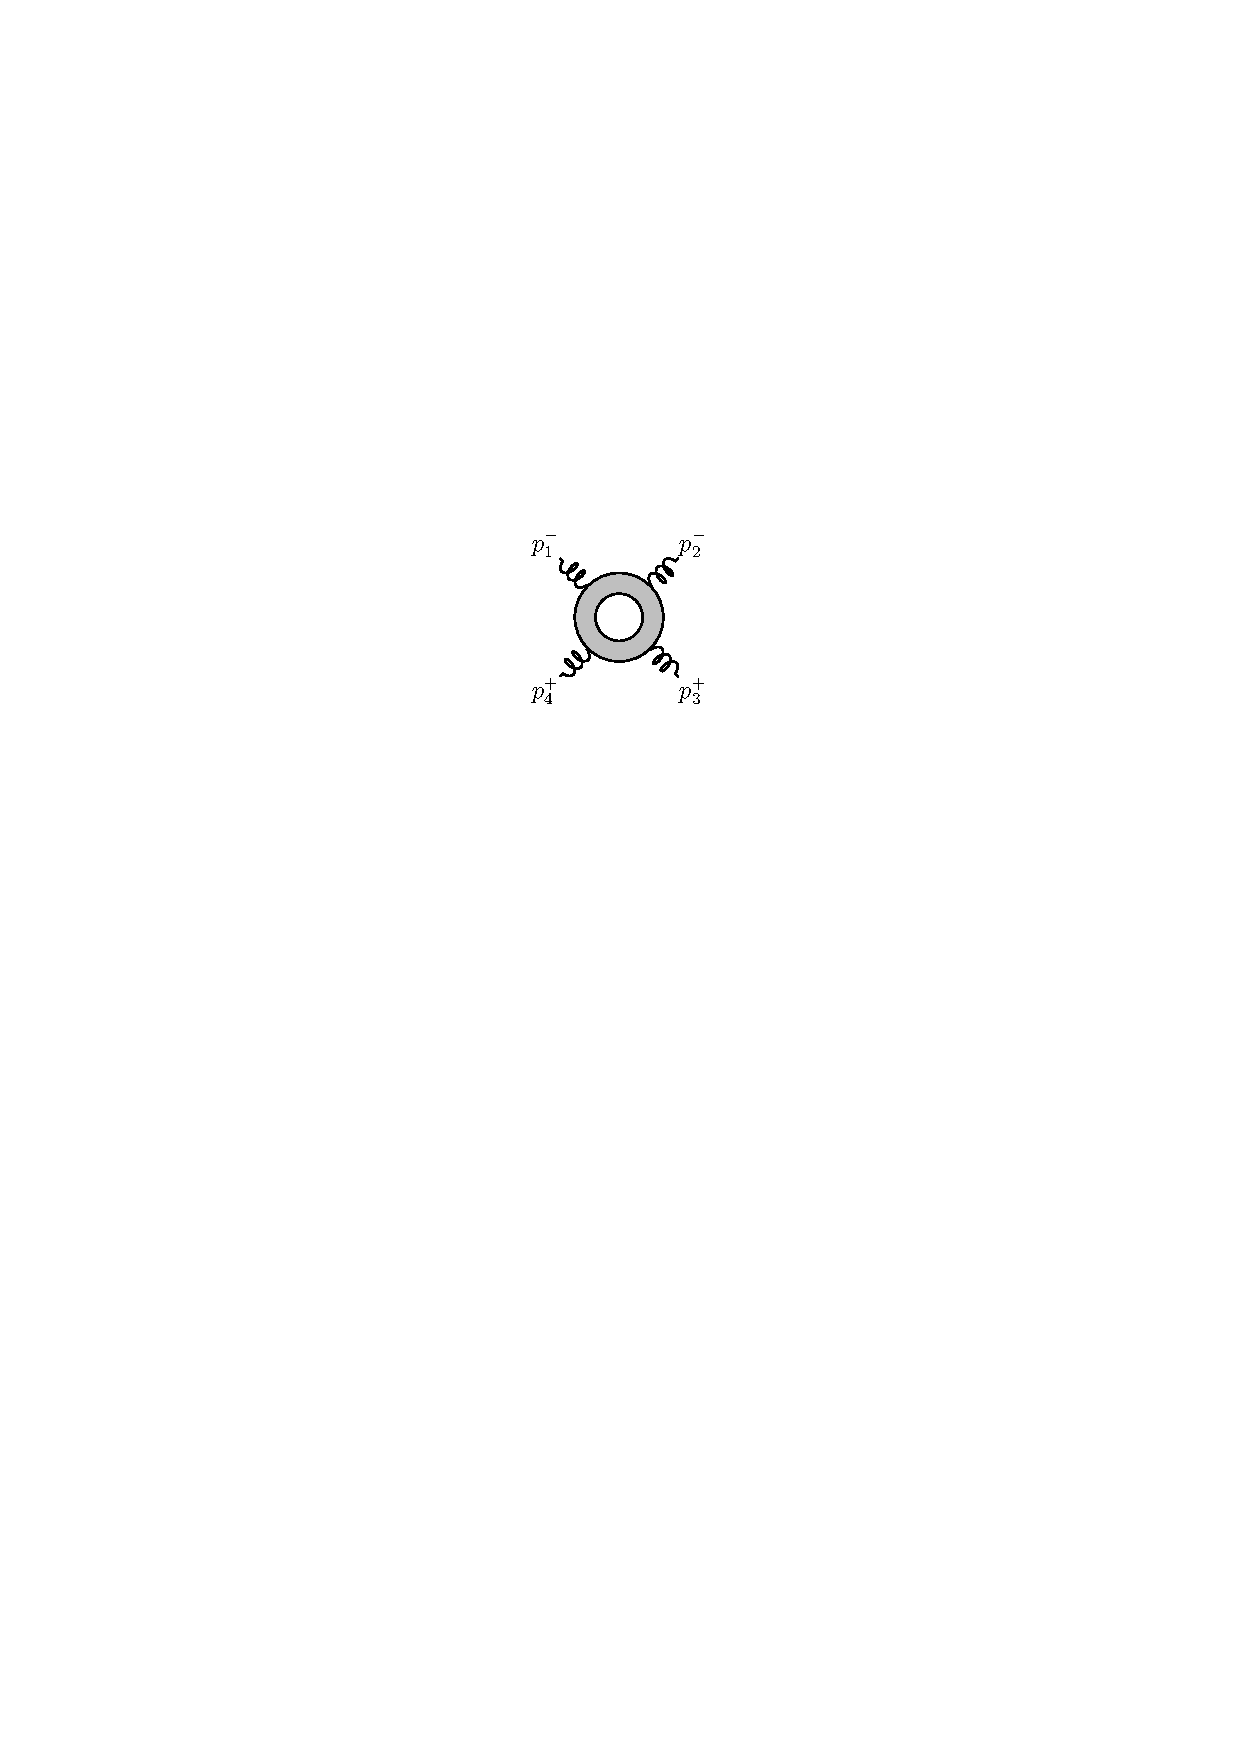
\includegraphics[width=2.5cm]{ch3_loopamps/figures/4g1Lampblob_MHV.pdf}} \right)
    \phantom{xx} = 
    \raisebox{-1.5cm}{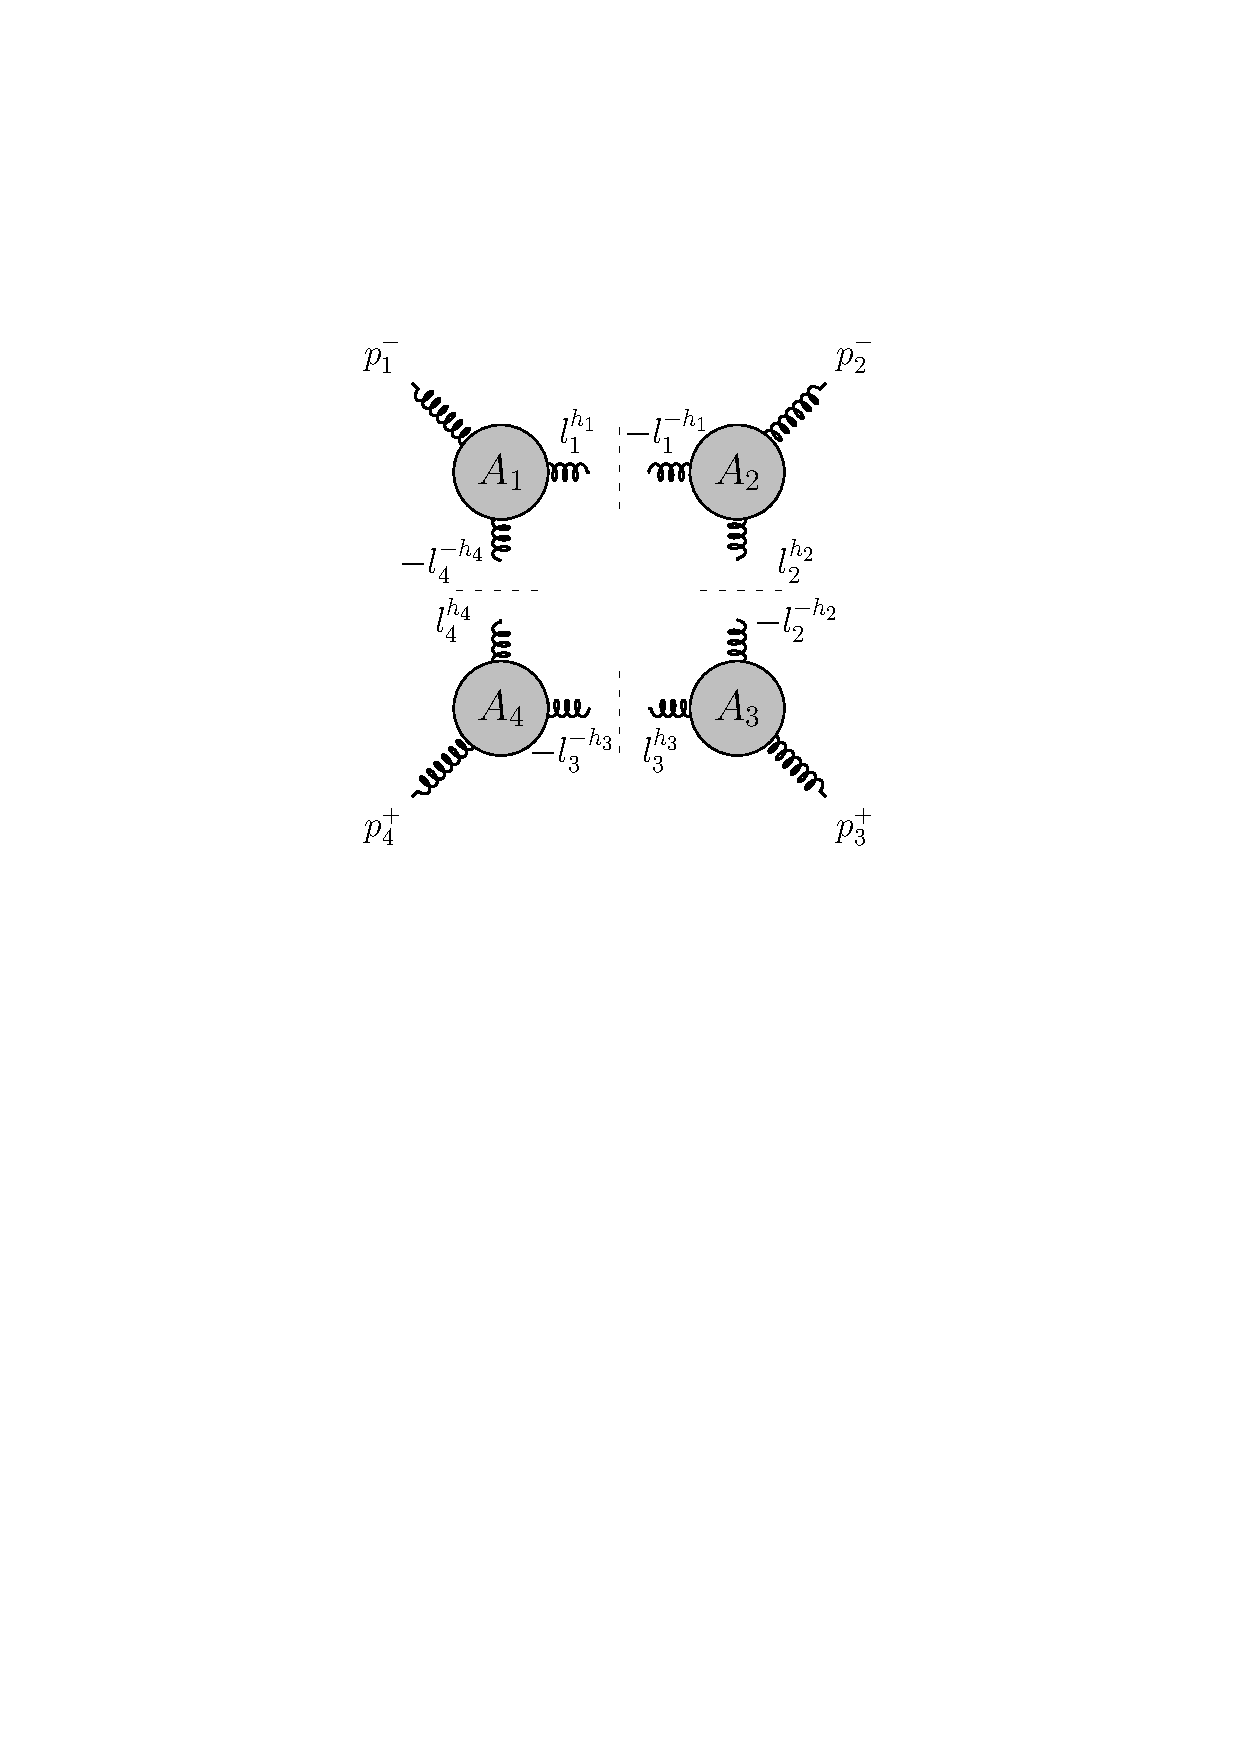
\includegraphics[width=3.5cm]{ch3_loopamps/figures/4g1L_gucut_genhels.pdf}}
    \label{eq:quadcut4g}
  \end{equation}
Each cut leads to a factorised product of trees where the sum over polarisation
states is implicit. The momenta in each of the four propagators, $l_i$, have
been put on-shell by solving the conditions $l_i^2 = 0$. To find an explicit
solution we can use a basis constructed from the spinors of the external
momenta such as
\begin{equation}
  l_1^\mu = \alpha_1 \, p_1^\mu + \alpha_2 \, p_2^\mu +  \alpha_3 \, \frac{1}{2}\spAB{1}{\gamma^\mu}{2} + \alpha_4 \, \frac{1}{2} \spAB{2}{\gamma^\mu}{1} \,.
  \label{eq:quadcutmombasis}
\end{equation}
Using momentum conservation, we re-write the four on-shell constraints as
\begin{align} \begin{aligned}
  l_1^2 &= 0 \,, \\
  l_2^2 &= (l_1-p_2)^2 = 0 \overset{l_1^2=0}{=} 2 \, l_1\cdot p_2 = 0 \,, \\
  l_3^2 &= (l_1-p_2-p_3)^2 = 0 \overset{
        \begin{subarray}{l}
          l_1^2=0\\
          l_2\cdot p_2=0
        \end{subarray}
       }{\Rightarrow} 2 \, l_1\cdot p_3 = s_{23} \,, \\
  l_4^2 &= (l_1+p_1)^2 = 0 \overset{l_1^2=0}{=} 2 \, l_1\cdot p_1 = 0 \,,
  \end{aligned}
  \label{eq:quadcuteqs1}
\end{align}
which then are easily translated into conditions on the coefficients $\alpha_i$,\footnote{The identities used perform the spinor-helicity algebra are given Section~\ref{sec:1.7}, in particular the Fierz identity in \eqn{eq:Fierz}. The reader may also refer to exercise~\ref{Ex:1.6} where the identity is proven.}
\begin{align} 
\label{eq:quadcuteqs2}
\begin{aligned}
  &\alpha_1\alpha_2 - \alpha_3\alpha_4 = 0 \,, \\
  &\alpha_1 s_{12} = 0 \,, \\
  &\alpha_1 s_{13} + \alpha_2 s_{23} + \alpha_3 \spAB132 + \alpha_4 \spAB231 = s_{23} \,, \\
  &\alpha_2 s_{12} = 0 \,.
 \end{aligned}
\end{align}
These must hold for generic external kinematics, i.e., for $s_{12} \neq 0 $ and $s_{23} \neq 0$ ($s_{13}=-s_{12}-s_{23}$ because of momentum conservation). 
The second and fourth equations in the system~\eqref{eq:quadcuteqs2} allow us to simplify the first constraint, which
becomes $\alpha_3 \alpha_4 = 0$, and so we see that there are exactly two
solutions to the quadruple cut on-shell conditions:
\begin{align}
  \vec{\alpha}^{(1)} &= \Bigl\{ 0, 0, \tfrac{\spA23}{\spA13} , 0 \Bigr\} \,, \\
  \vec{\alpha}^{(2)} &= \Bigl\{ 0, 0, 0, \tfrac{\spB23}{\spB13} \Bigr\} \,,
  \label{eq:quadcutsol}
\end{align}
where we introduced the short-hand notation $\vec{\alpha} = \{\alpha_1,\alpha_2,\alpha_3,\alpha_4\}$.
These solutions deserve a few remarks. We see that the two solutions are
complex, and in fact are complex conjugates of each other. In order to extract
the value of the quadruple cut we will sum and average over the two solutions
as well as the sum over helicity in the factorised product of trees. For now we
simply state that this is the correct method to obtain the scalar integral
coefficient, though we will return to prove this later in
section~\ref{ssec:4dintegrandbasis}. The fact that the loop momenta are complex
means we must analytically continue the factorised tree-level amplitudes for
complex momenta as well.\footnote{The on-shell delta functions in the cut
integrals should also be reinterpreted as residue computations.} This step is
quite familiar to us, since we have already encountered analytic continuation
of tree amplitudes in the context of BCFW recursion. However, we should not
underestimate the importance of having a well defined analytic continuation. In
fact this feature was one of the main obstacles in the analytic $S$-matrix
program of the~1960's.

Turning back to our example, all that remains to do is to substitute the
on-shell solutions into the tree-amplitude expressions. Since these tree-level
amplitudes will be of the form of Parke-Taylor MHV amplitudes, it is first
convenient to write explicit spinor solutions for the the loop momenta $l_i$.
There is a flexibility in how to do this because of the little group symmetry,
but a simple choice using $z = {\spA23}/{\spA13}$ is
\begin{align} \begin{aligned}
  |l_1^{(1)} \r> &= |1\r> \,, & |l_1^{(1)}] &= z \, |2] \,, \\
  |l_2^{(1)} \r> &= z\, |1\r> - |2\r> \,, \qquad \quad & |l_2^{(1)}] &= |2] \,, \\
  |l_3^{(1)} \r> &= z\, |1\r> - |2\r> \,, & |l_3^{(1)}] &= \frac{s_{23}}{z \, s_{12}}\bigl(|1] + z \, |2]\bigr) \,, \\
  |l_4^{(1)} \r> &= |1\r> \,, & |l_4^{(1)}] &= |1] + z |2] \,,
  \end{aligned}
  \label{eq:quadcutsolspinors}
\end{align}
for the first solution, while the second is obtained by complex conjugation (i.e.\ replacing $|\r>
\leftrightarrow |]$ which also means $z\leftrightarrow z^\dagger$). Other choices of spinor normalisation will not affect the
final answer.

\begin{figure}[h]
  \centering
  \begin{tabular}[h]{cc}
    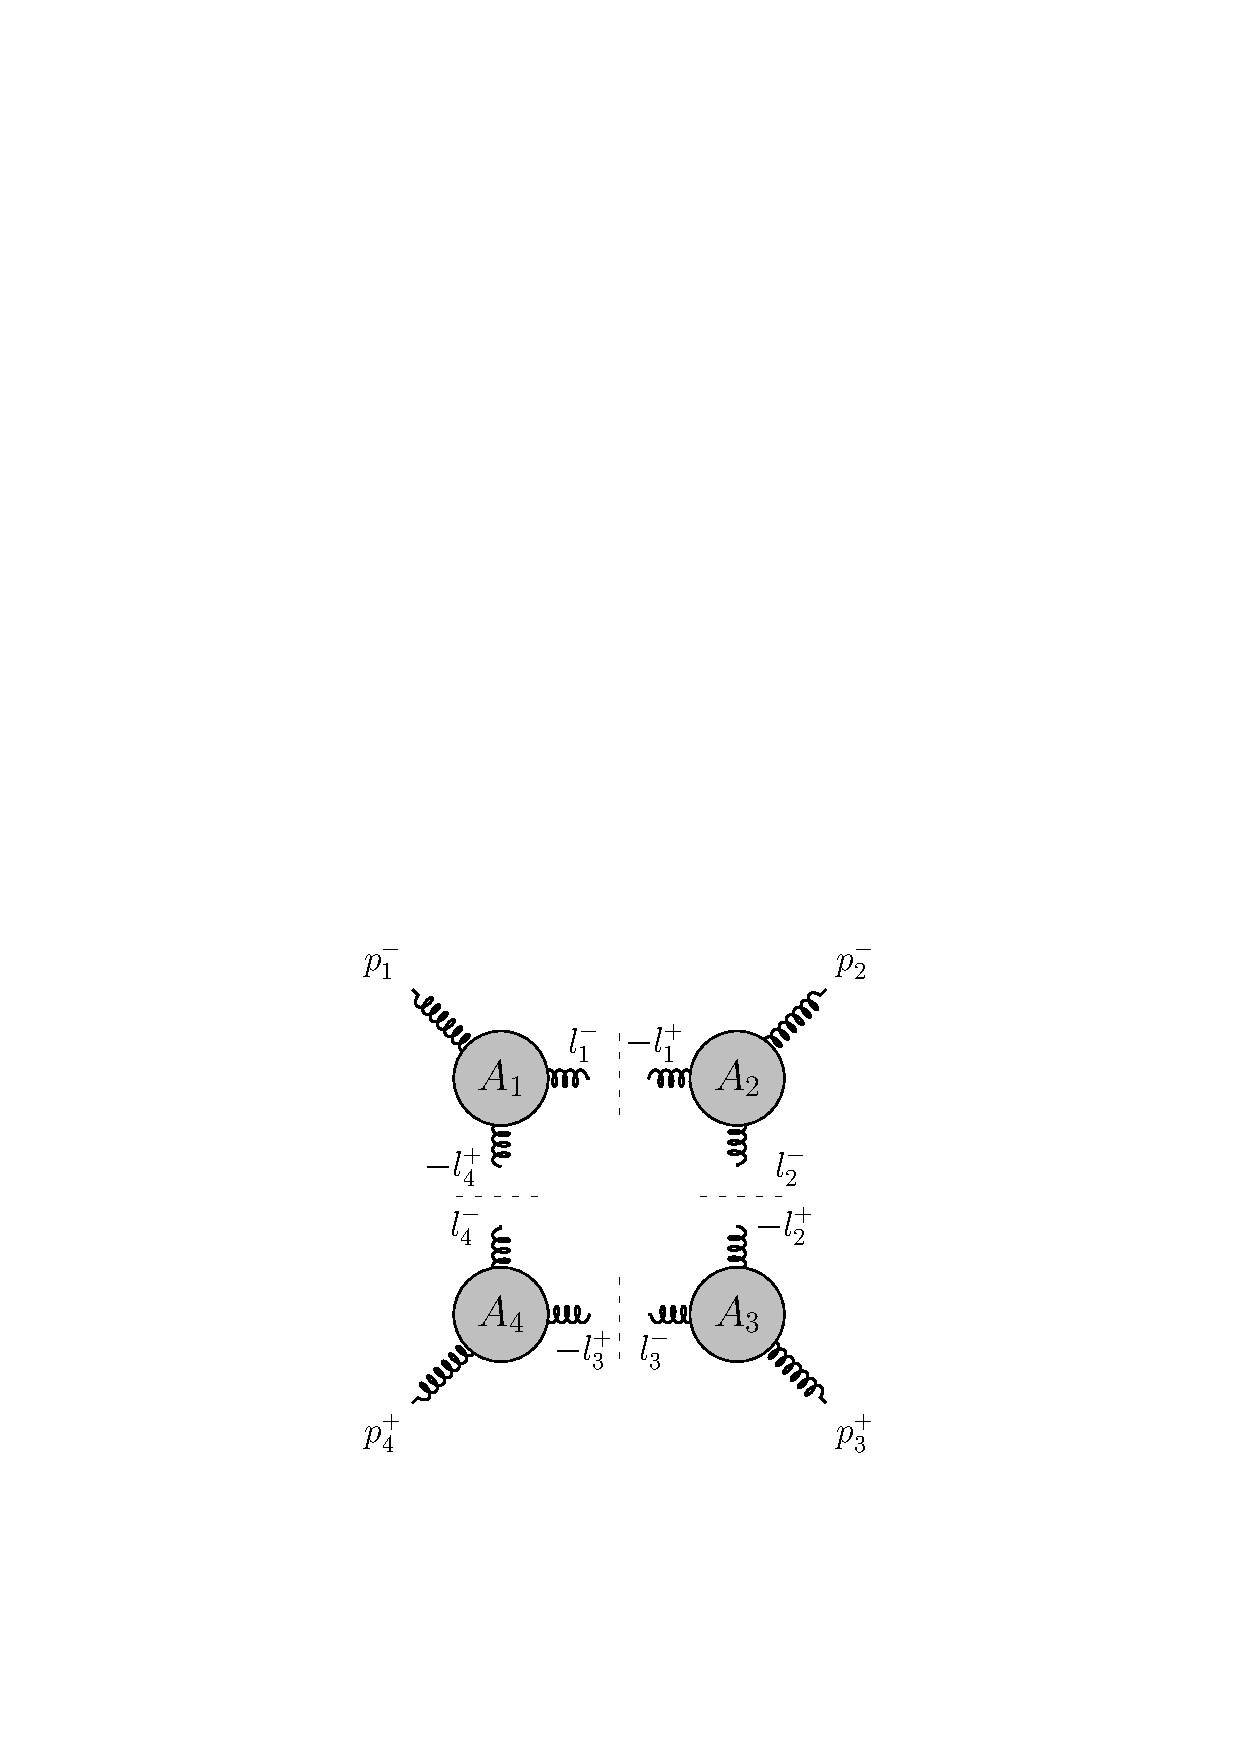
\includegraphics[width=4cm]{ch3_loopamps/figures/4g1L_gucut_exhels.pdf} &
    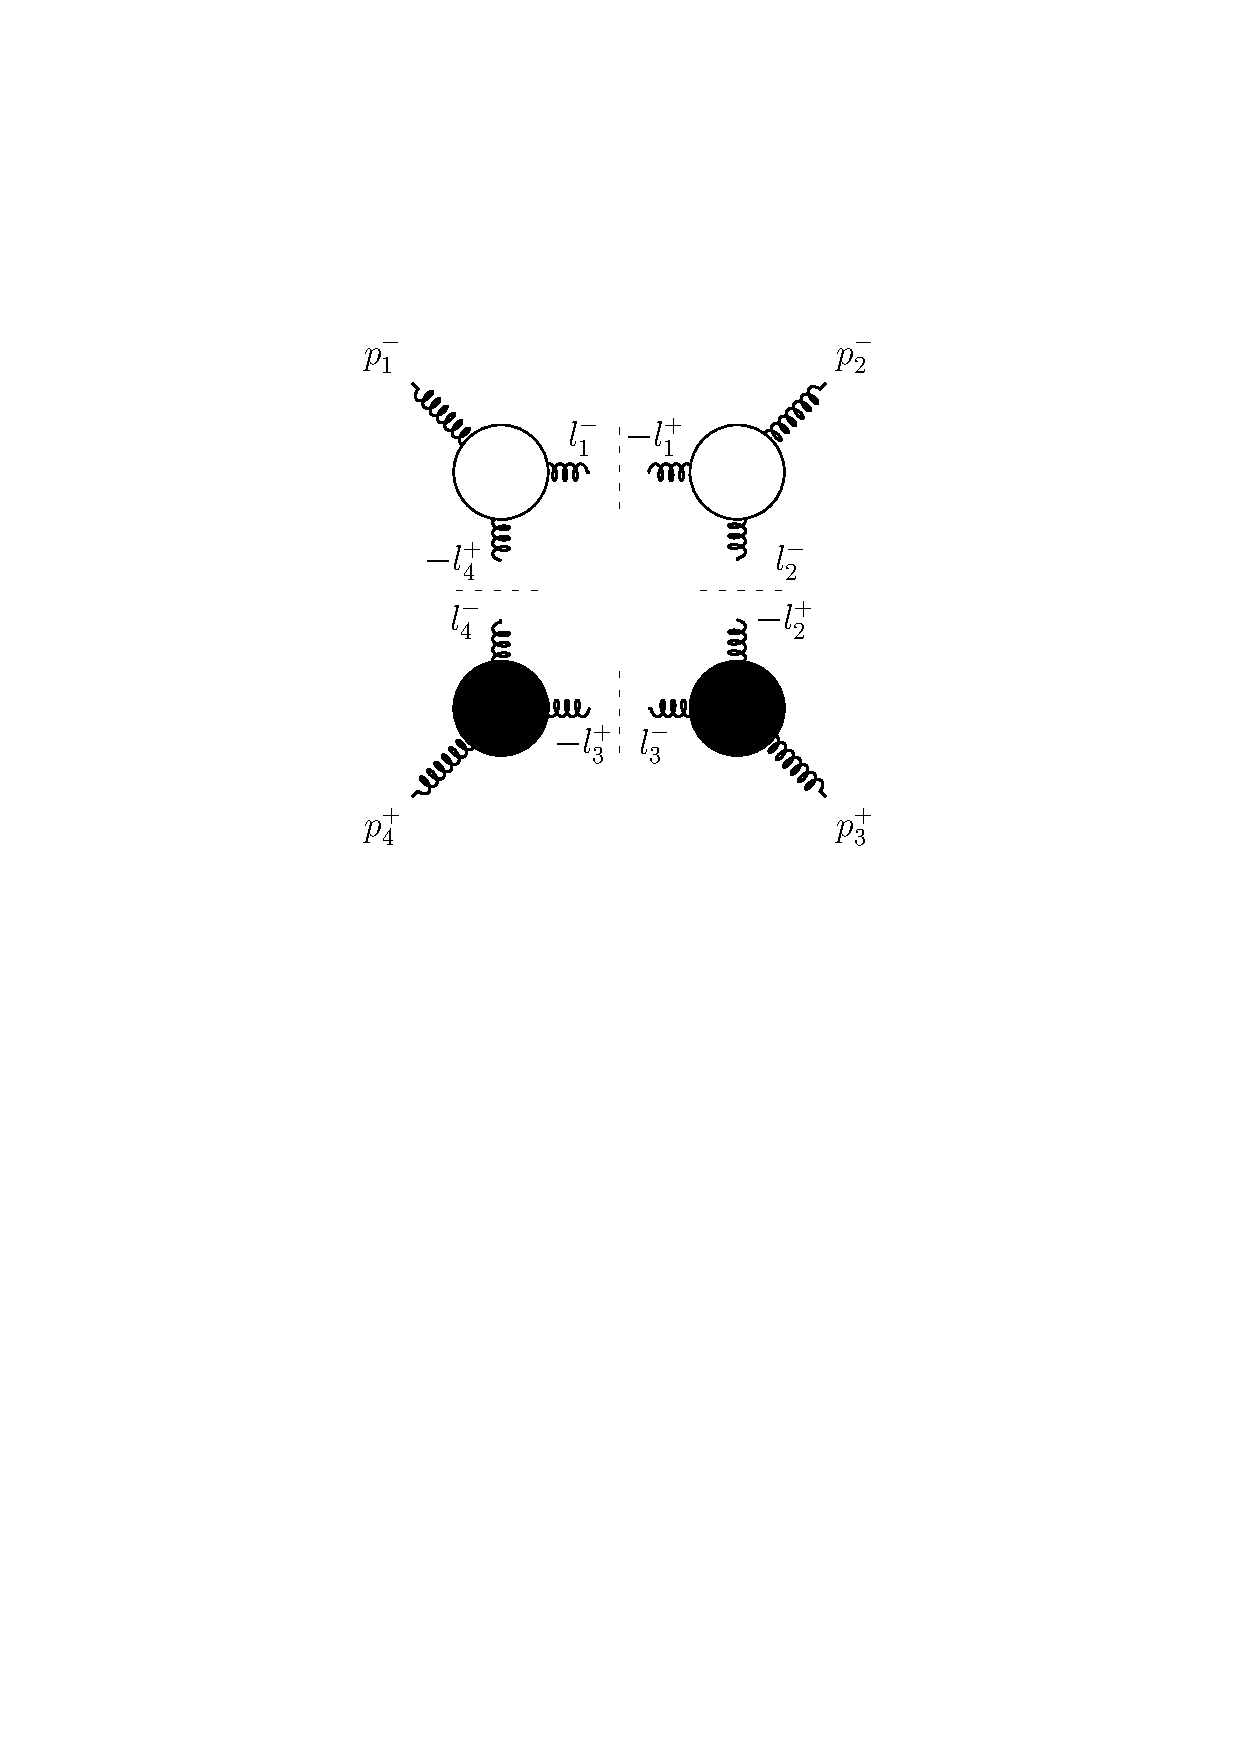
\includegraphics[width=4cm]{ch3_loopamps/figures/4g1L_gucut_exhels_shaded.pdf}
  \end{tabular}
  \caption{An example helicity configuration contributing to the quadruple cut of the four gluon MHV amplitude. In the right panel the configuration is shown with MHV-type vertices shaded in white and \MHVb vertices shaded in black.}
  \label{fig:4gcutexhel}
\end{figure}

We are now ready to start substituting the on-shell solutions into the
expressions for the tree amplitudes. Let us start with the configuration of
internal helicities shown in figure \ref{fig:4gcutexhel}. Each of the
three-point amplitudes is either MHV or $\overline{\rm MHV}$. The first
amplitude at the top left of the cut evaluated on the first on-shell solution
is
\begin{equation}
  A_1  = \i \, \frac{\spA1{l_1}^3}{\spA{l_1}{(-l_4)}\spA{(-l_4)}{l_1}} \,,
  \label{eq:4ggucutexhel1}
\end{equation}
from which it is simple to see $A_1|_{l_i^{(1)}} = 0$, since the spinor solution
in \eqn{eq:quadcutsolspinors} shows the angle spinor for $l_1$ is
proportional to the angle spinor of $p_1$. One may worry about the remaining
spinor products in the denominator since they can also be shown to vanish on
the solution $l_1^{(1)}$, but the overall dimension of the three-point amplitude
ensures that $A_1|_{l_i^{(1)}}$ is indeed zero. There is a similar story for the
solution $l_1^{(2)}$, where we see that, since $|l_1^{(2)}\r> \propto |2\r>$, then
$A_2|_{l_1^{(2)}} = 0$. As a result we find no contribution from this helicity
configuration. This is a general feature of quadruple cuts for massless theories,
and we can use the fact that three-point amplitudes contain only angle or square
brackets to conclude:
\begin{important}{Three-point vertex rule for unitarity cuts.}
  Unitarity cuts of one-loop amplitudes do not support adjacent MHV (or \MHVb) three-point vertices.
\end{important}
A popular and convenient graphical notation is to shade the three-point
vertices to indicate whether they are of either MHV (white) or \MHVb~(black),
as shown in the right panel of Figure~\ref{fig:4gcutexhel}, which demonstrates that
this internal helicity configuration vanishes since we have highlighted
adjacent MHV amplitudes. Applying this rule to the full helicity
sum leads us to find only two non-vanishing contributions, one for each of the
two solutions:
\begin{align}
  \mathcal{C}_{1|2|3|4} \left(  \raisebox{-1.3cm}{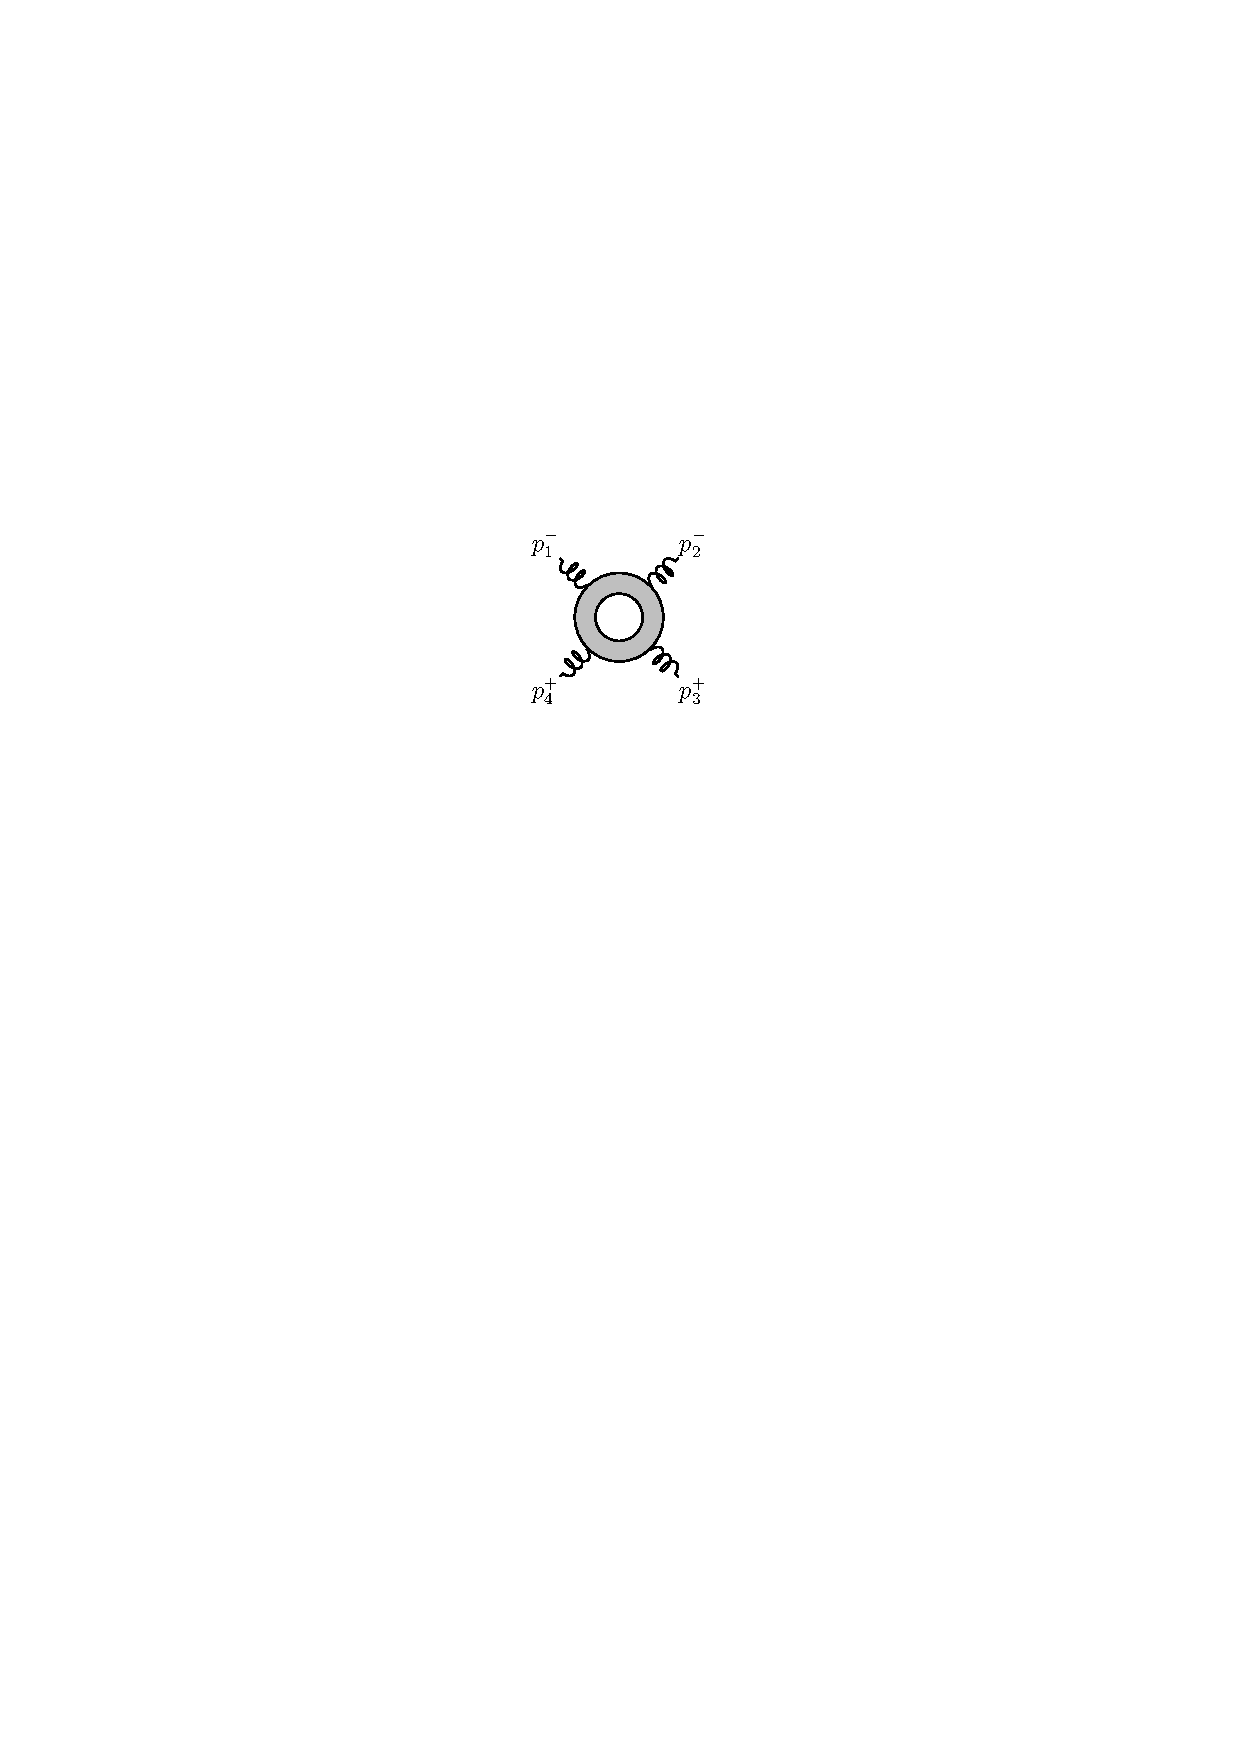
\includegraphics[width=2.5cm]{ch3_loopamps/figures/4g1Lampblob_MHV.pdf}} \right) \Bigg|_{l_i^{(1)}}
    \phantom{xx} &=
    \raisebox{-1.7cm}{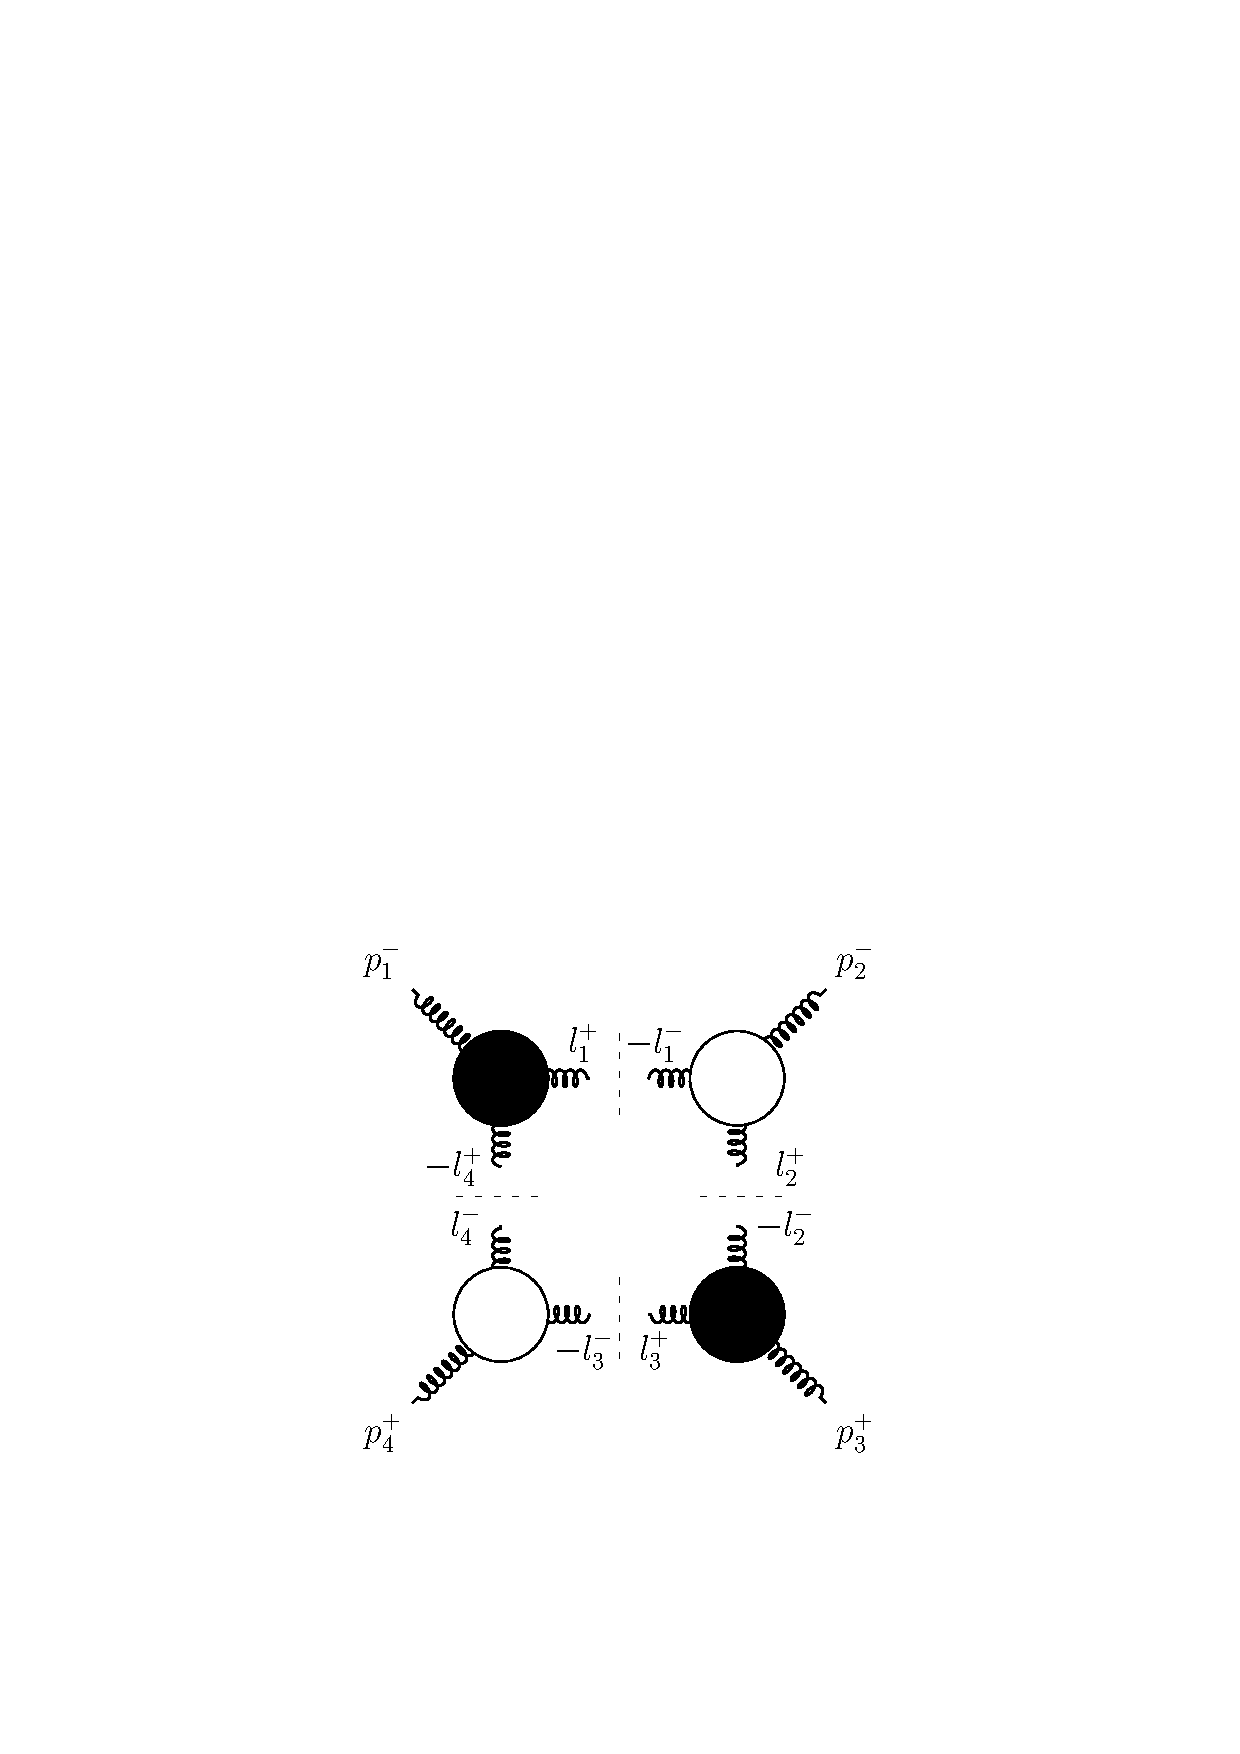
\includegraphics[width=3.5cm]{ch3_loopamps/figures/4g1L_gucut_hel1.pdf}} \Bigg|_{l_i^{(1)}} \,, \\
  \mathcal{C}_{1|2|3|4} \left(  \raisebox{-1.3cm}{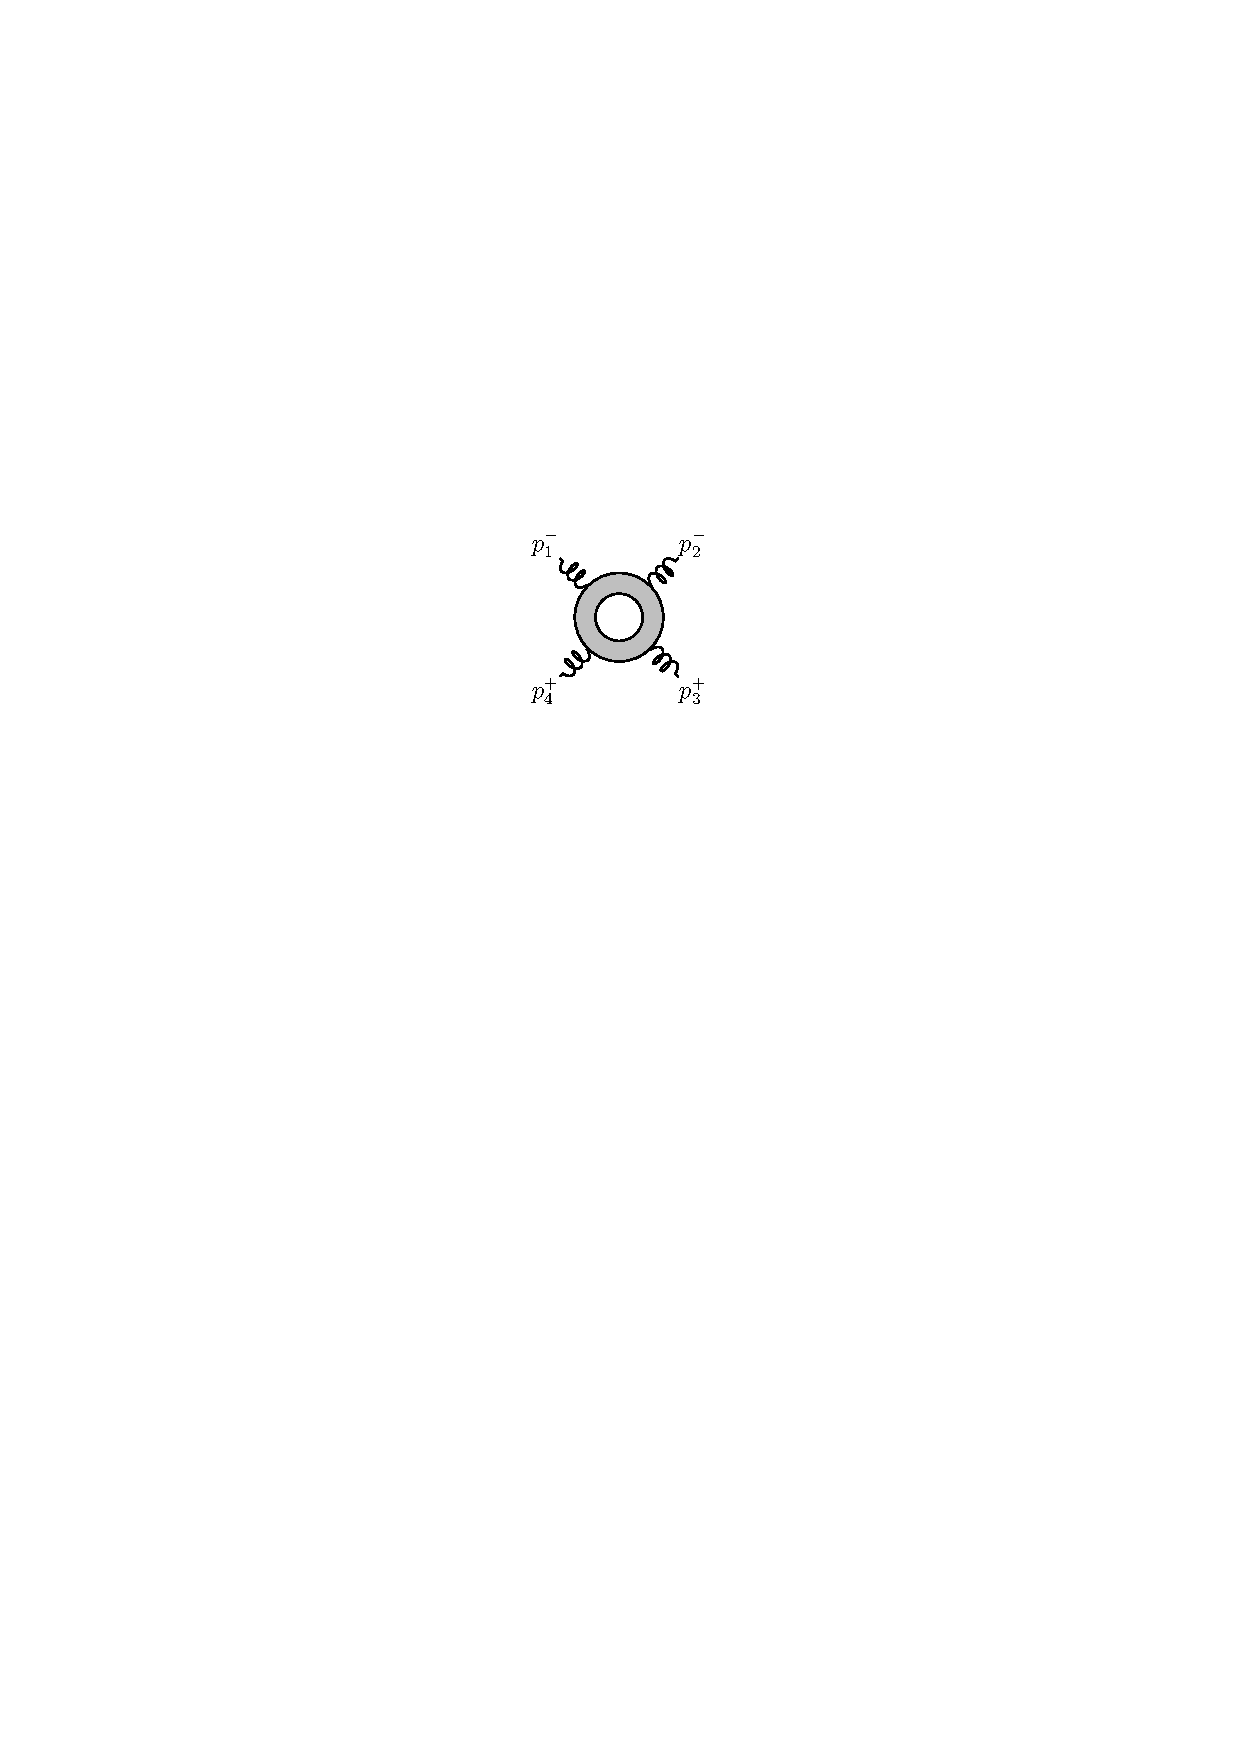
\includegraphics[width=2.5cm]{ch3_loopamps/figures/4g1Lampblob_MHV.pdf}} \right) \Bigg|_{l_i^{(2)}}
    \phantom{xx} &=
    \raisebox{-1.7cm}{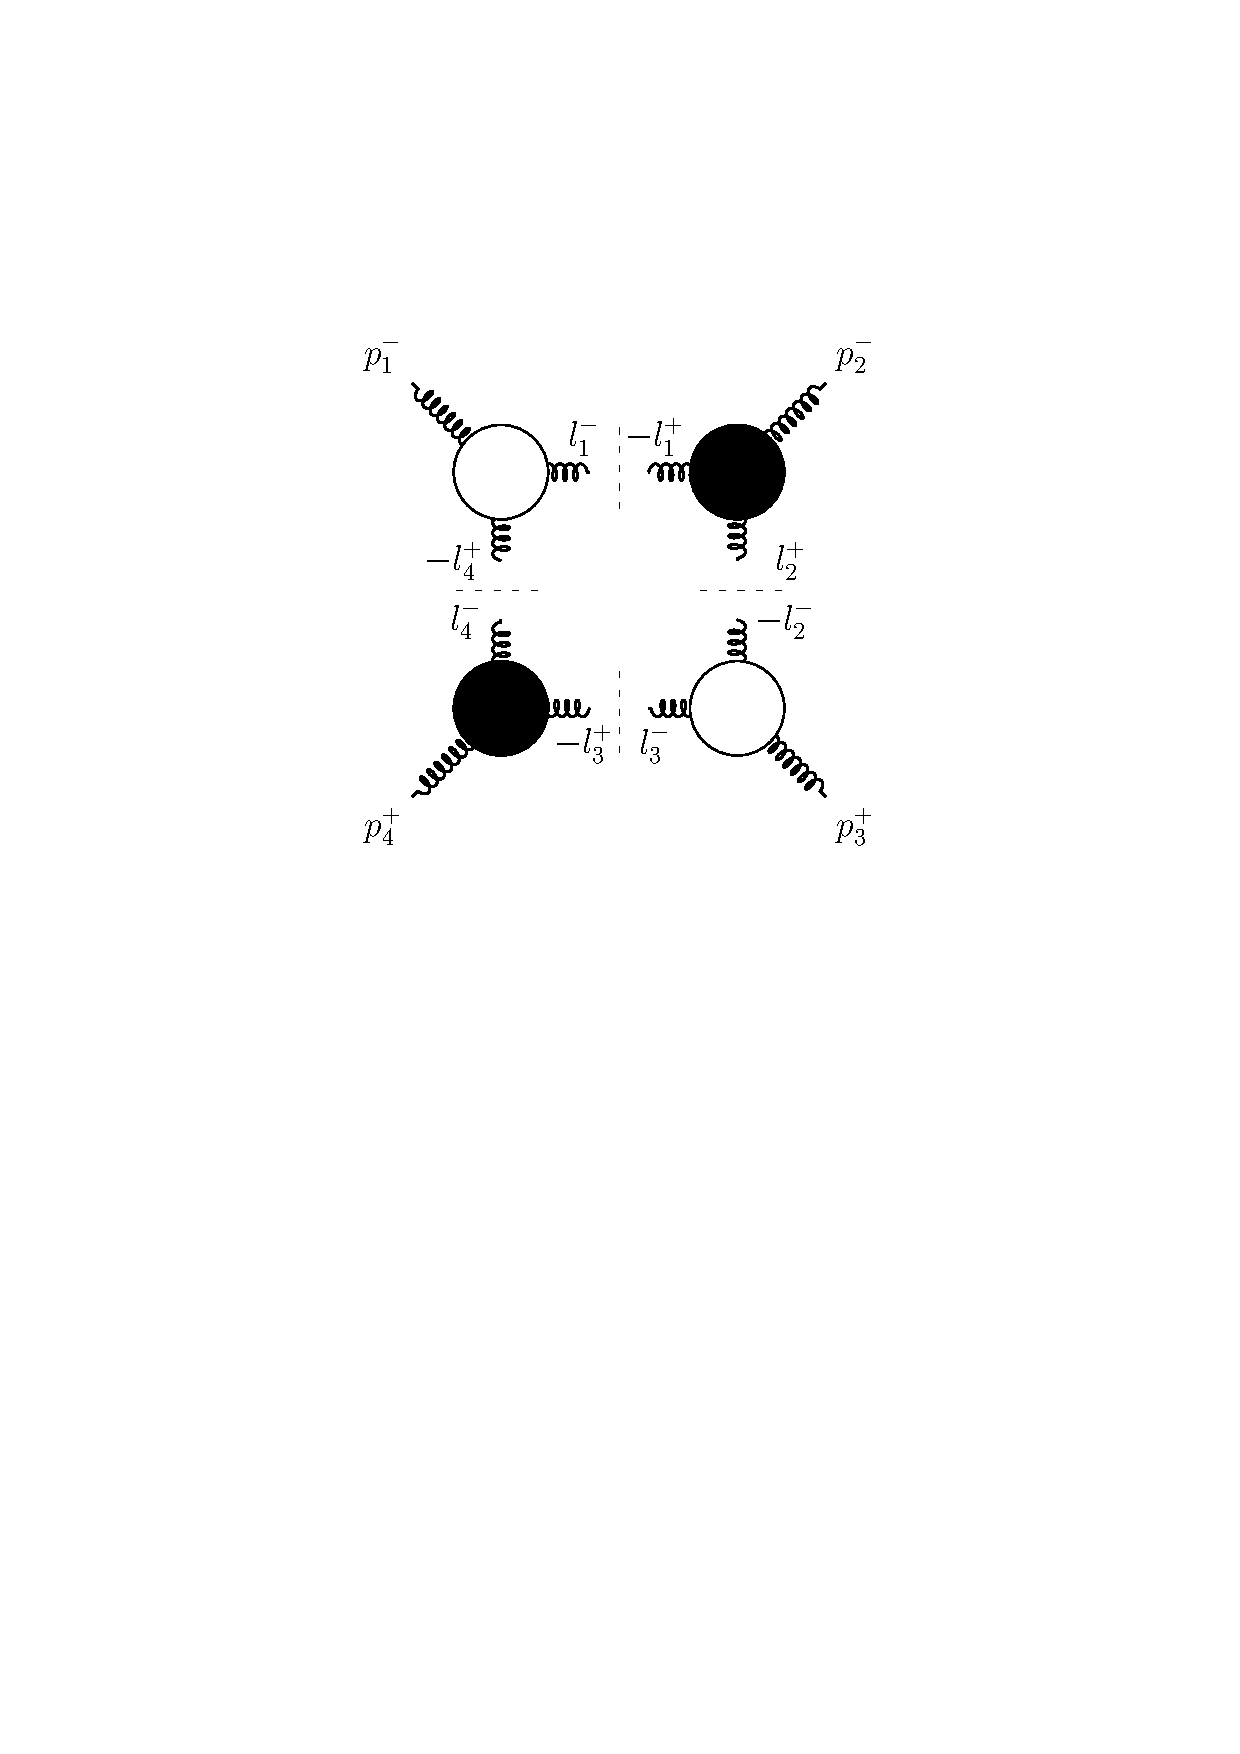
\includegraphics[width=3.5cm]{ch3_loopamps/figures/4g1L_gucut_hel2.pdf}} \Bigg|_{l_i^{(2)}} \,.
  \label{eq:4gcutnonvanishinghels}
\end{align}

We can now complete the computation of the quadruple cut:
\begin{align}
    \raisebox{-1.5cm}{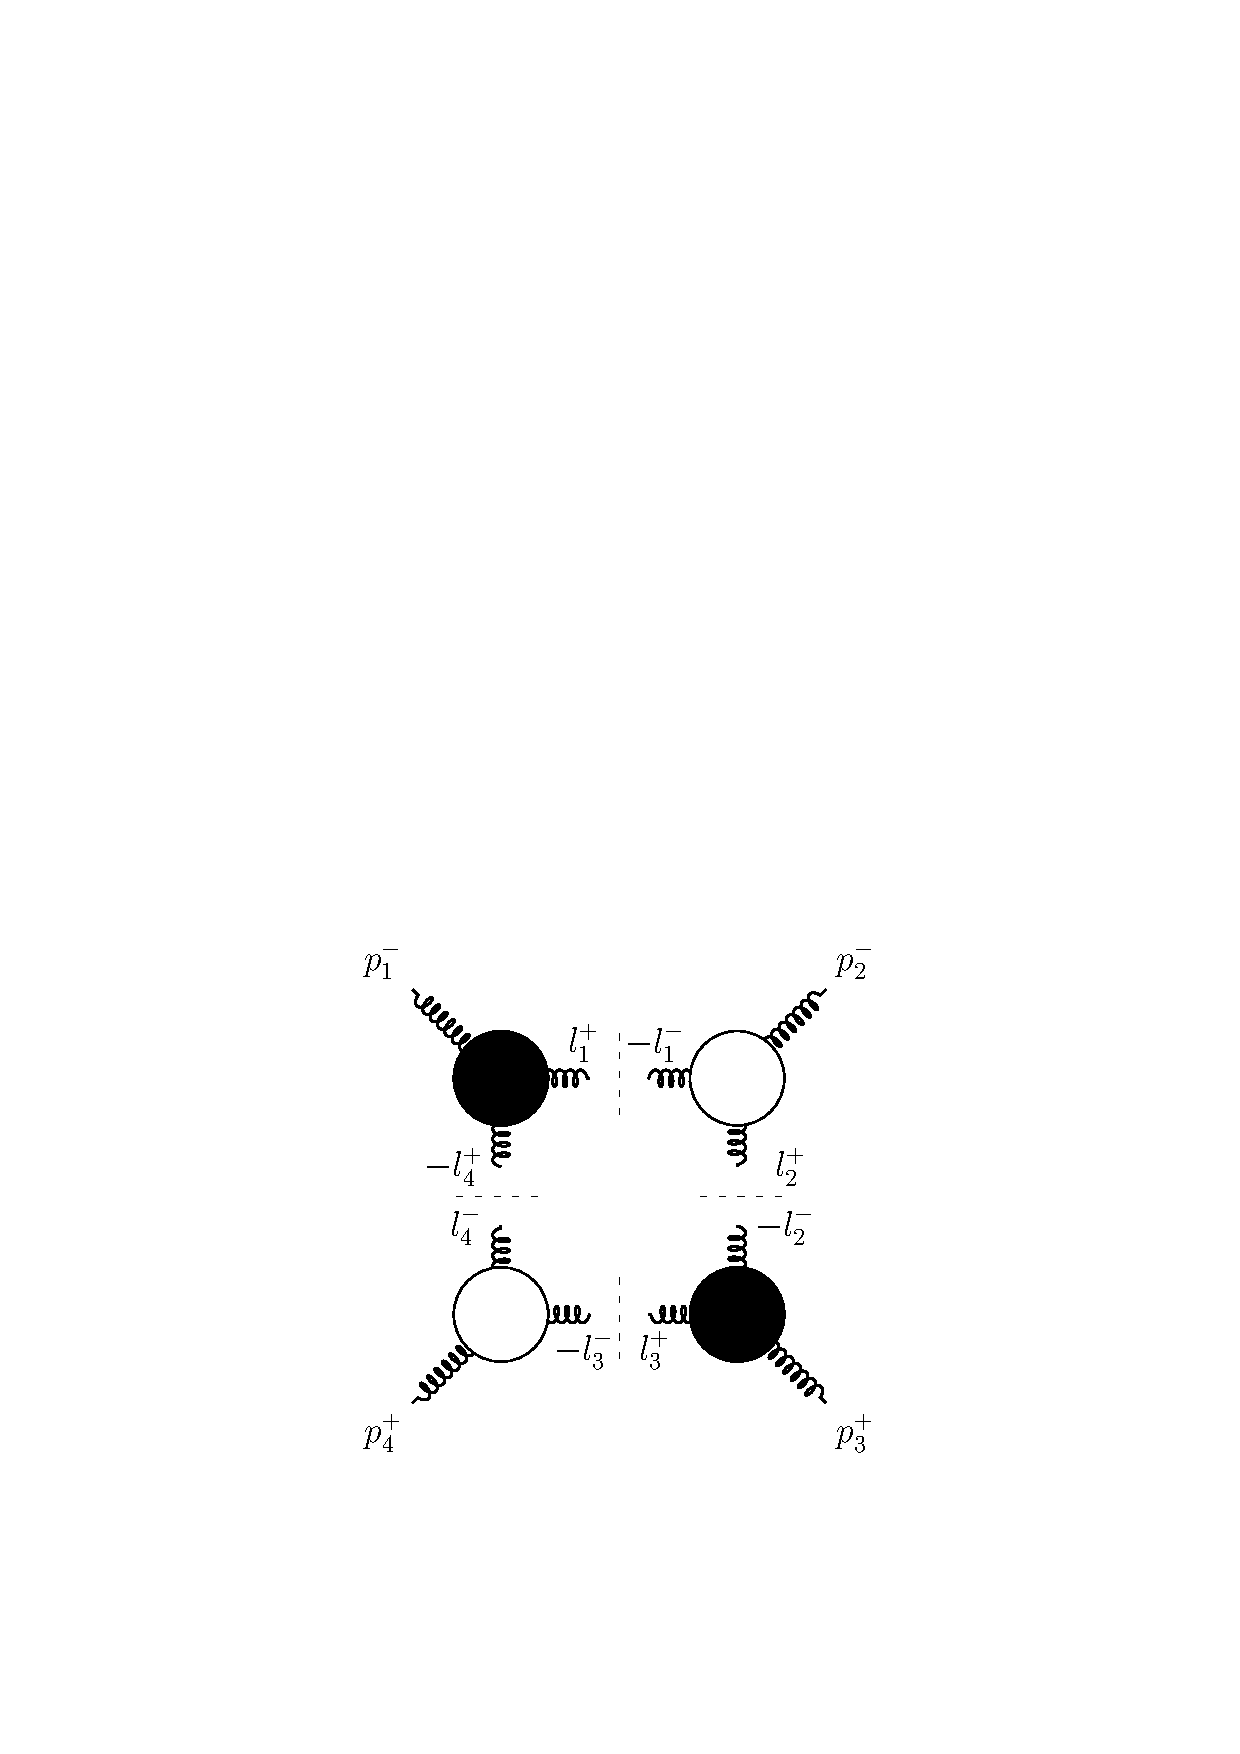
\includegraphics[width=3cm]{ch3_loopamps/figures/4g1L_gucut_hel1.pdf}} \Bigg|_{l_i^{(1)}}
    =
    \frac{\spB{l_1}{l_4}^3}{\spB{l_4}{1}\spB{1}{l_1}}
    \frac{\spA{l_1}{2}^3}{\spA{2}{l_2}\spA{l_2}{l_1}}
    \frac{\spB{3}{l_3}^3}{\spB{l_3}{l_2}\spB{l_2}{3}}
    \frac{\spA{l_3}{l_4}^3}{\spA{l_4}{4}\spA{4}{l_3}} \bigg|_{l_i^{(1)}}\,.
  \label{eq:4gcutresidue1a}
\end{align}
Substituting \eqn{eq:quadcutsolspinors} for $l_1, l_2$ and $l_4$ gives
\begin{align}
    \raisebox{-1.5cm}{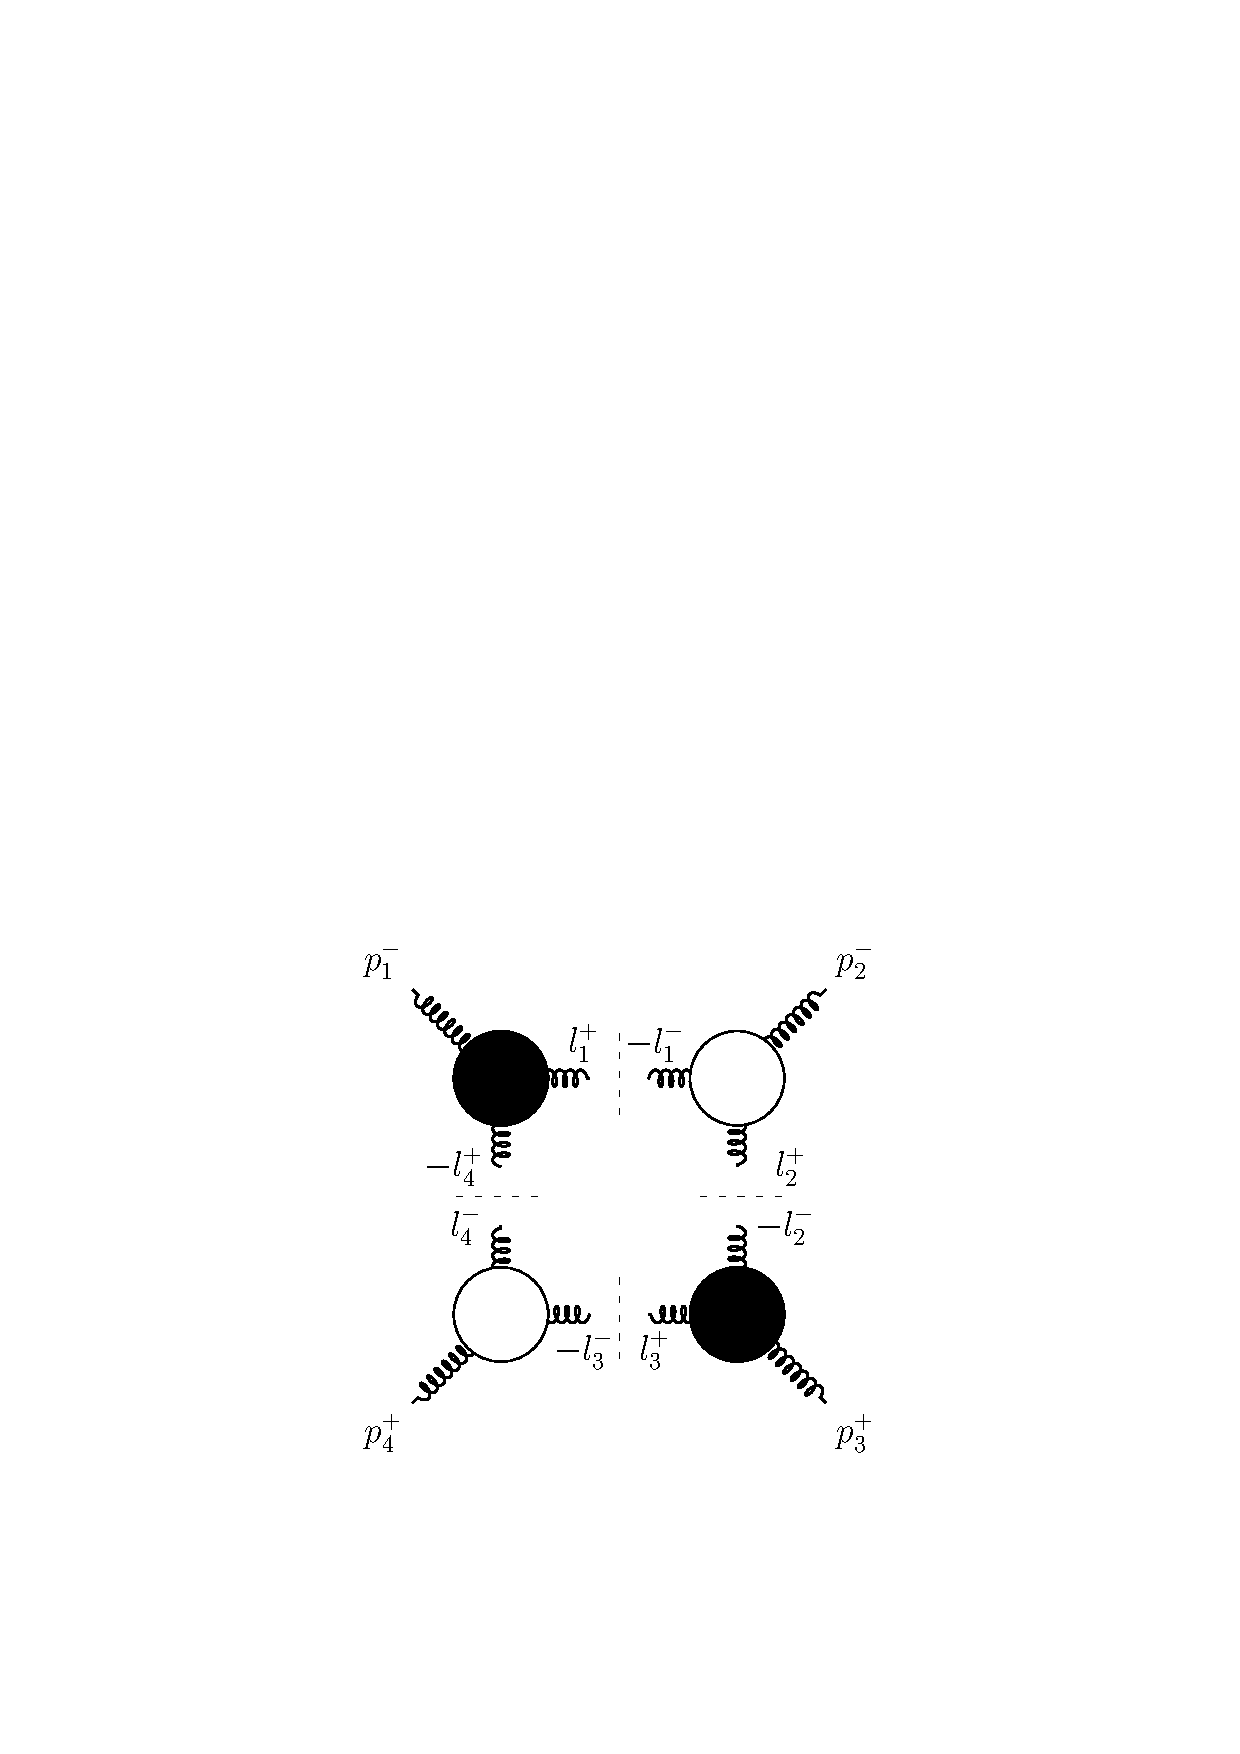
\includegraphics[width=3cm]{ch3_loopamps/figures/4g1L_gucut_hel1.pdf}} \bigg|_{l_i^{(1)}}
    \hspace{-0.3cm} =
    \frac{(z\spB21)^3}{(z\spB21)(z\spB12)}
    \frac{\spA12^3}{(z\spA21)(-\spA21)}
    \frac{\spB{3}{l_3}^3}{\spB{l_3}{2}\spB23}
    \frac{\spA{l_3}{1}^3}{\spA14\spA{4}{l_3}} \Bigg|_{l_i^{(1)}}\,.
  \label{eq:4gcutresidue1b}
\end{align}
The substitution of $l_3$ would require some spinor manipulation at first sight but the spinor products can be combined together to make ``sandwiches'' of the $l_3$ momentum,
after which where we can evaluate using momentum conservation:
\begin{equation}
  \frac{\spB{3}{l_3}^3}{\spB{l_3}{2}}\frac{\spA{l_3}{1}^3}{\spA{4}{l_3}} \bigg|_{l_i^{(1)}} = \frac{\spAB1{l_3}3^3}{\spAB4{l_3}2} \bigg|_{l_i^{(1)} } = \frac{\spA12^3\spB23^3}{\spA43\spB32} = \frac{\spA12^3\spB23^2}{\spA34} \,.
  \label{eq:l3sub1}
\end{equation}
Putting everything together, we find the final result is simply\footnote{As is always the case with spinor algebra there are many paths to reach the same final result. Here we have attempted to be very explicit but the reader may prefer alternative derivations. For example, by expanding in the spinor basis for $p_1$ and $p_2$ we broke some symmetry in the original configuration. One can apply some more algebra to show that $|l_3^{(1)}\r> = |3\r>, |l_3^{(1)}] = \tfrac{\spA14}{\spA13} |4]$ for example, in which we would get a simple result without first combining into spinor sandwiches.}
\begin{align}
    \raisebox{-2cm}{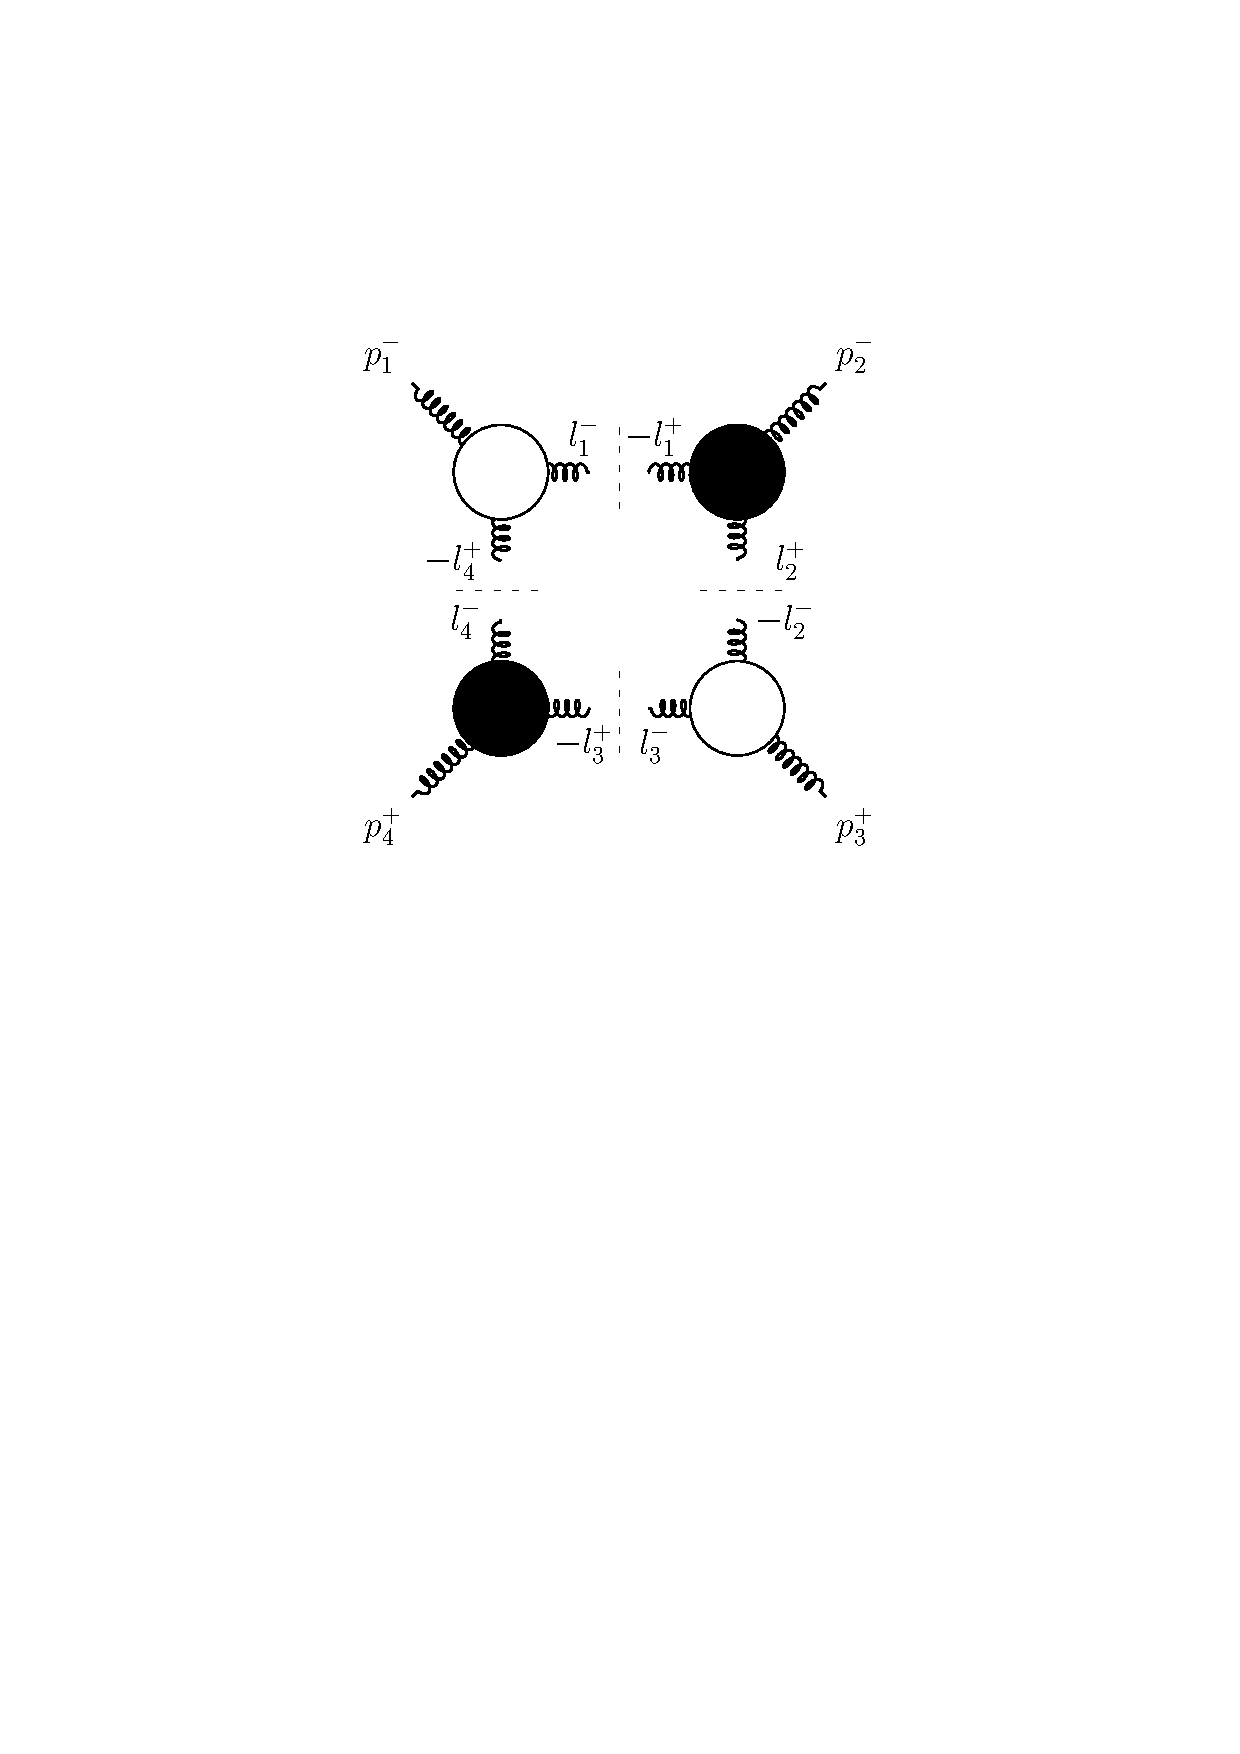
\includegraphics[width=4cm]{ch3_loopamps/figures/4g1L_gucut_hel2.pdf}} \Bigg|_{l_i^{(2)}} 
    = -s_{12} s_{23} \bigl(-\i A^{(0)}(1^-,2^-,3^+,4^+) \bigr) \,.
\end{align}
A similar computation for the other non-zero cut configuration leads to
\begin{align}
    \raisebox{-2cm}{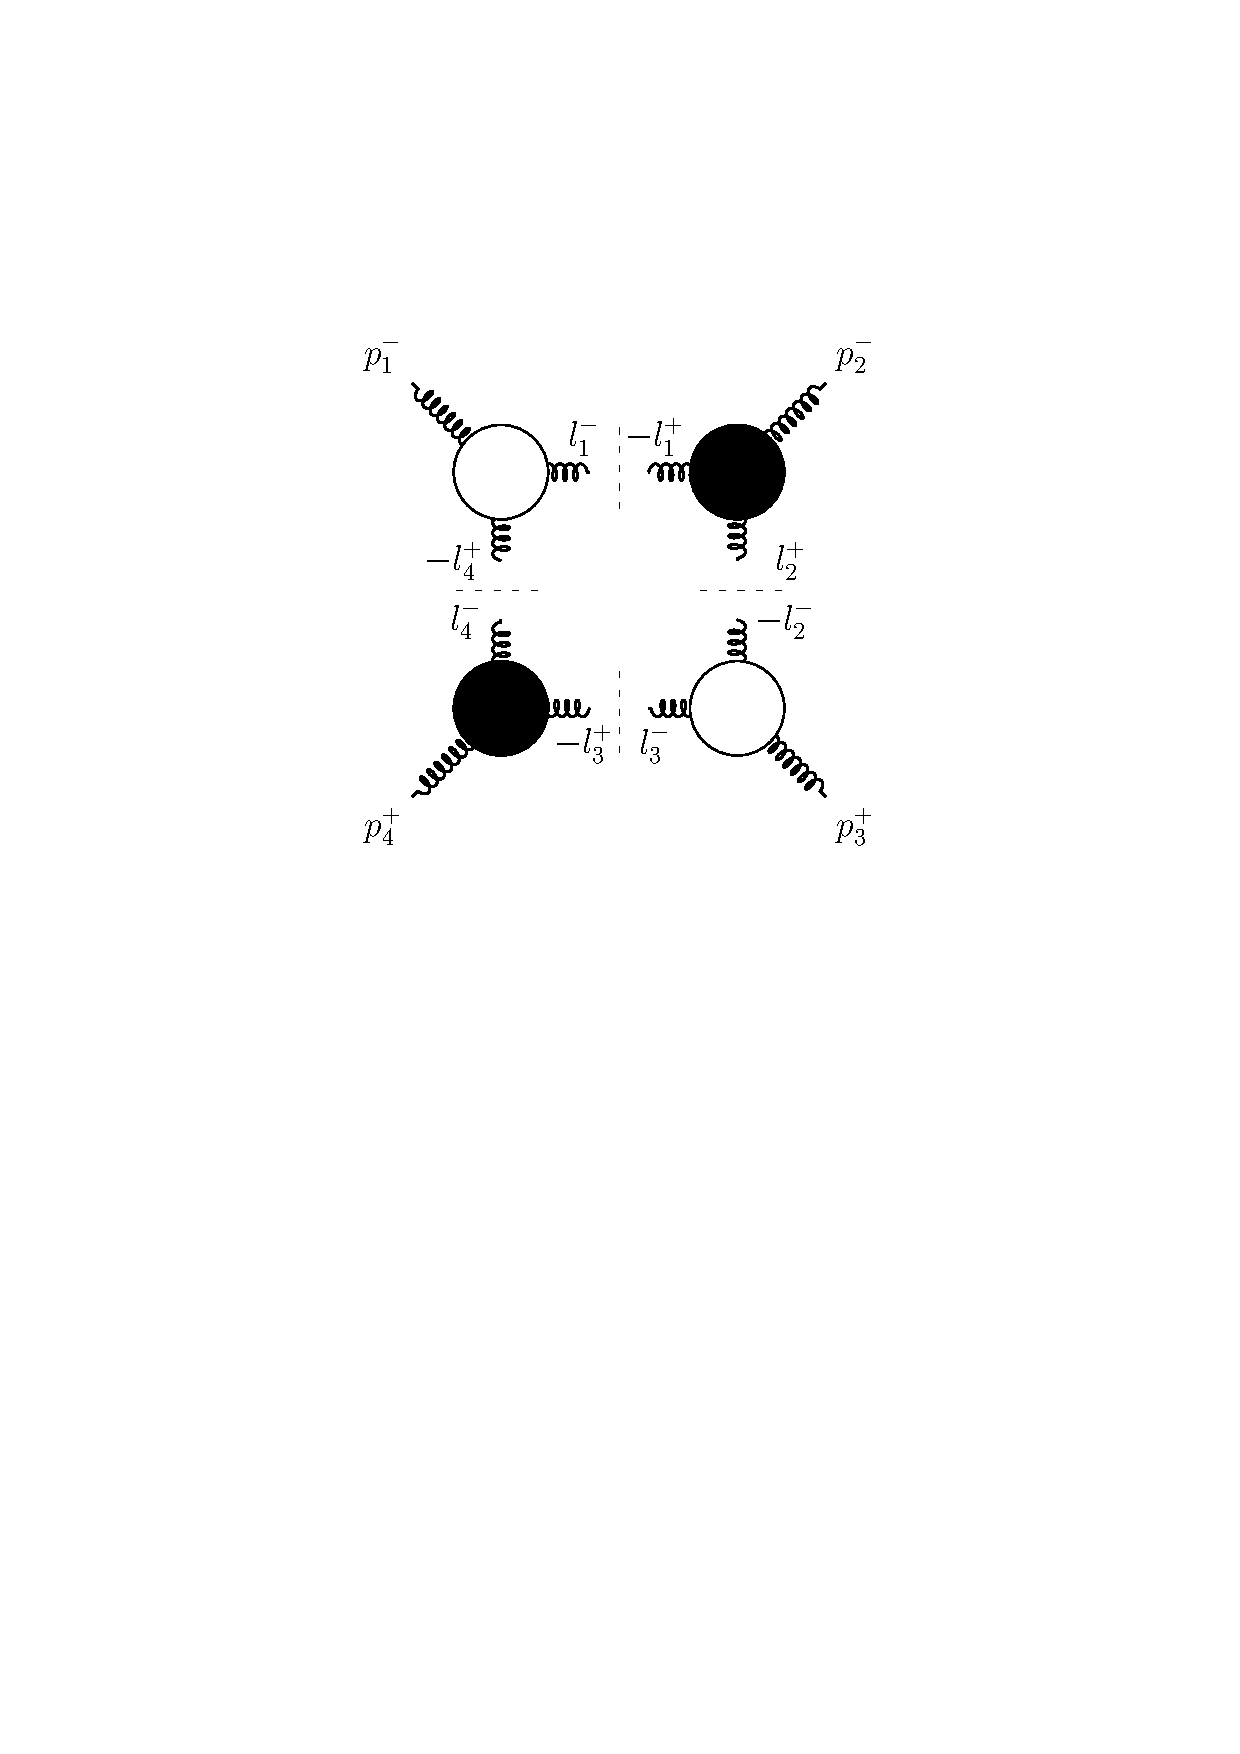
\includegraphics[width=4cm]{ch3_loopamps/figures/4g1L_gucut_hel2.pdf}} \Bigg|_{l_i^{(2)}} 
    = -s_{12} s_{23} \bigl(-\i A^{(0)}(1^-,2^-,3^+,4^+) \bigr) \,.
\end{align}
The coefficient of the scalar box integral is the average of the two solutions, and so we recover the result observed from the double cuts, that is
\begin{equation}
  A^{(1)}(1^-,2^-,3^+,4^+) =  \i \, c_{0;1|2|3|4}(1^-,2^-,3^+,4^+) \, F_4^{[D]}(s_{12},s_{23}) + \text{subtopologies}\,,
\end{equation}
where
\begin{align}
  c_{0;1|2|3|4}(1^-,2^-,3^+,4^+) &= \frac{1}{2} \sum_{s=1}^2 \mathcal{C}_{1|2|3|4}\left( I^{(1)}(1^-,2^-,3^+,4^+) \right) \Bigl|_{l_i^{(s)}} \nonumber \\
  &= -s_{12} s_{23} \bigl(-\i \, A^{(0)}(1^-,2^-,3^+,4^+)\bigr) \,.
  \label{eq:4gquadcutfinal}
\end{align}

\end{example}

\begin{exer}{Quadruple cuts of five-gluon MHV scattering amplitudes}
\label{Ex:3.2}
\vspace{-0.6cm}
\begin{enumerate}[a)]
\item  Follow the method of quadruple cuts for the one-loop five-gluon amplitudes to show that
\begin{equation}
  c_{0;1|2|3|45}(1^-,2^-,3^+,4^+,5^+) = \frac{\i}{2} s_{12} s_{23} A^{(0)}(1^-,2^-,3^+,4^+,5^+) \,.
\end{equation}
\item A more complicated example is required to show that we will not always find that box coefficients are proportional to tree-level amplitudes. Using the same technique, show that
\begin{align}
\begin{aligned}
   c_{0;1|23|4|5}(1^+,2^+,3^-,4^+,5^-) = & \, \frac{\i}{2}  s_{45} s_{15} \, A^{(0)}(1^+,2^+,3^-,4^+,5^-) \\
  & \times \left[ \left( \frac{\spA34 \spA15}{\spA14 \spA35} \right)^4 + \left( \frac{\spA13 \spA45}{\spA14 \spA35} \right)^4 \right]  \,.
 \end{aligned}
\end{align}
\end{enumerate}
For the solution see \hyperref[Sol:3.2]{chapter~5}.
\end{exer}

\section{Reduction methods \label{sec:3.4}}

Through the concepts of unitarity and generalised unitarity cuts we have been
able to understand better the meaning of equation \eqref{eq:loopamp-general}.
While performing two-particle cuts, we saw that the cut-constructible part of
the four-gluon MHV amplitude could be written in terms of a scalar box integral
and sub-topologies written in terms of triangle and bubble integrals with some
non-trivial numerator function. In this section will we show how to reduce this
loop dependent tensor numerators to basis integral functions. We will then see how we can extend these ideas to find a basis of integrand level structures. 

\subsection{Tensor reduction}
\label{sec:TensorReduction}

This approach to the computation of one-loop amplitudes due to Passarino and
Veltman~\cite{ch3_Passarino:1978jh} revolutionised the field of precision theoretical predictions for high
energy experiments. The method is remarkably and elegantly simple. We will
restrict ourselves to massless propagators as before although the method is
equally applicable in the general case. Consider a tensor integral such as
\begin{equation}
  F_n^{[D]}(p_1,\ldots,p_{n-1})[k^\mu] = \int_k \frac{k^\mu}{\prod_{a=1}^{n}[-(k-q_a)^2]} \,,
  \label{eq:tensorintexample}
\end{equation}
where $q_{a} = \sum_{b=1}^{a-1} p_b$ as before. Feynman's $\i 0$ prescription is irrelevant for the purpose of this section, hence we omit it. After integration the
integral can only depend on the independent external momenta, and so the vector can be described by a linear combination of $n-1$ external
momenta, as
\begin{equation}
  F^{[D]}_{n}[k^\mu] = \sum_{i=1}^{n-1} a_{n,i} \, p_i^\mu \,,
  \label{eq:testintexampledecomp}
\end{equation}
where we have dropped the momentum argument on the LHS for a more
compact notation. The coefficients $a_{n,i}$, referred to as \emph{form factors}, can then be determined by
constructing a linear system of equations through contractions of eqs.~\eqref{eq:tensorintexample} and~\eqref{eq:testintexampledecomp} with the basis
vectors $p_i$. For illustrative purposes it is useful to take a specific
example, say $n=2$ with $p_1^2\neq 0$. We then find one equation,
\begin{align}
  \int_k \frac{k\cdot p_1}{k^2 (k-p_1)^2} = a_{2,1} \, p_1^2 \,.
\end{align}
By rewriting the scalar product in the numerator in terms of inverse propagators through
 $2 \, k\cdot p_1 = k^2 - (k-p_1)^2 + p_1^2$, we can expand the LHS into three scalar integrals,
\begin{align}
  \frac{1}{2} \int_k \frac{1}{(k-p_1)^2}  - \frac{1}{2} \int_k \frac{1}{k^2} + \frac{p_1^2}{2} \int_k \frac{1}{k^2 (k-p_1)^2} = a_{2,1} \, p_1^2 \,.
\end{align}
The first two scalar integrals on the LHS have the topology of a tadpole. Since they do not depend on any external scale, they are zero in dimensional regularisation,\footnote{We will come back to this non-trivial aspect in chapter~\ref{ch:loopints}.} and so we arrive at the well known result
\begin{align}
  a_{2,1} = \frac{1}{2} F^{[D]}_2(p_1)[1] \,.
  \label{eq:PVbubR1sol}
\end{align}
For a general tensor we can decompose into bases of external momenta and the metric tensor, for example,
\begin{align}
  F^{[D]}_{2}[k^{\mu_1}k^{\mu_2}] &=  \int_k \frac{k^{\mu_1} k^{\mu_2}}{k^2 (k-p_1)^2} = a_{2,00} \, \eta^{\mu_1\mu_2} + a_{2,11} \, p_1^{\mu_1} p_1^{\mu_2}  \,,\label{eq:PVbubR2dec}\\
  F^{[D]}_{2}[k^{\mu_1}k^{\mu_2} k^{\mu_3}] &=  \int_k \frac{k^{\mu_1} k^{\mu_2}k^{\mu_3}}{k^2 (k-p_1)^2} \nonumber\\
  & = a_{2,001} \left( \eta^{\mu_1\mu_2} p_1^{\mu_3} + \eta^{\mu_2\mu_3} p_1^{\mu_1} + \eta^{\mu_3\mu_1} p_1^{\mu_2} \right) \nonumber\\
  & \phantom{= {}} + a_{2,111} \, p_1^{\mu_2} p_1^{\mu_2} p_1^{\mu_3} \,.
\label{eq:PVbubR3dec}
\end{align}
Note that the final example is a rank-three two-point function, which would not
appear in a conventional renormalisable gauge theory, which permits a maximum
tensor rank of $n$ for a $n$-point one-loop function. This follows from the
restrictions on the mass dimension of the operators that represent the
interactions leading to a general counting of one power of momentum per
three-point vertex. This is not the case for gravity theories (see section~\ref{sec:1.4}) or effective field theories.

Explicit solutions for the form factors are easy to find with an automated computer algebra
system, although for higher-point integrals can quickly generate large
expressions and complicated denominators from the determinant of the linear
system of equations. These are known as \emph{Gram determinants}, since they are
related to the Gram matrix computed from the independent external momenta, that is, the matrix of entries
$[G_n]_{ij} = p_i \cdot p_j$ with $i,j=1,\ldots,n-1$.

There are many references in which well organised analytic solutions are presented, see~\cite{ch3_Ellis:2011cr} and references therein for a summary. 
Many of these have seen extensive use in high energy physics applications. We leave the complete solution to the bubble system as an exercise.

\begin{exer}{Tensor decomposition of the bubble integral}
\label{Ex:3.3}
\vspace{-0.6cm}
\begin{enumerate}[a)]
\item Prove that the form factors in the decomposition of the rank-two bubble integral in \eqn{eq:PVbubR2dec} are given by
\begin{align} \label{eq:rank2bubsol}
\begin{aligned}
  a_{2,00} &= -\frac{p_1^2}{4(D-1)} \, F_2^{[D]}(p_1)[1] \,, \\
  a_{2,11} &= \frac{D}{4(D-1)} \, F_2^{[D]}(p_1)[1] \,.
\end{aligned}
\end{align}

\item Prove that the form factors in the decomposition of the rank-three bubble integral in \eqn{eq:PVbubR3dec} are given by
\begin{align} \label{eq:rank3bubsol}
\begin{aligned}
  a_{2,001} &= -\frac{p_1^2}{8(D-1)} \, F_2^{[D]}(p_1)[1] \,, \\
  a_{2,111} &= \frac{D+2}{8(D-1)} \, F_2^{[D]}(p_1)[1] \,.
\end{aligned}
\end{align}
\end{enumerate}
For the solution see \hyperref[Sol:3.3]{chapter~5}.
\end{exer}

\begin{example}{Example: Reducing the $gg\to gg$ $s_{23}$-channel cut to scalar integrals}

At the end of section~\label{sec:3.2} (eqs.~\eqref{eq:tchannelcut1}--\eqref{eq:tchannelcut3})
we reached an expression for the $s_{23}$-channel double cut of the four-gluon MHV
amplitudes written in terms of cut Feynman integrals. The box contribution was
already in a reduced form, while the triangle and bubble sub-topologies had
non-trivial dependence in the numerator. Since we will use many different
generalised cuts, we use the notation from section~\ref{sec:3.3} for the
quadruple cut $\mathcal{C}_{1|2|3|4}$, also for the double cuts
$\mathcal{C}_{I|J}$, triple cuts $\mathcal{C}_{I|J|K}$, and so on. The
$s_{12}$-channel cut of a four-particle process is therefore represented as
$\mathcal{C}_{12|34}$, and $\mathcal{C}_{23|41}$ represents the $s_{23}$-channel cut.
Written explicitly in terms of the integral functions $F_n^{[D]}$ the result is
\begin{align} \label{eq:4gcut23recall}
  \mathcal{C}_{23|41}&\left( A^{(1)}(1^-,2^-,3^+,4^+) \right)
    = \mathcal{C}^{\rm box}_{23|41} + \mathcal{C}'_{23|41} \,,
\end{align}
where\footnote{Note that we have changed the double cut to apply to the amplitude rather than the integrand in this section, which affects the factors of $\i$.}
\begin{align}
 & \mathcal{C}^{\rm box}_{23|41} = - A^{(0)}(1^-,2^-,3^+,4^+) \, s_{12} s_{23} \, \mathcal{C}_{23|41}\left( F_4^{[D]}(p_2,p_3,p_4) \right) \,, \\
 \label{eq:4gcut23recallCprime}
 &  \mathcal{C}'_{23|41} = - 2 A^{(0)}(1^-,2^-,3^+,4^+) \, \frac{1}{s_{12}^2s_{23}^2} \times \nonumber\\
  & \quad \mathcal{C}_{23|41} \left(
    F_2^{[D]}(p_{23})[\mathcal{N}_2 ]
  + \frac{1}{s_{12}} F_3^{[D]}(p_{23},p_4)[\mathcal{N}_{3,a}]
  + \frac{1}{s_{12}} F_3^{[D]}(p_2,p_3)[\mathcal{N}_{3,b}]
  \right)\,. 
\end{align}
Here the non-trivial numerators are given by
\begin{align}
  \mathcal{N}_2 &= \trmgamtwo1{\slashed{l}_2}32^2 + s_{12}s_{23} \, \trmgamtwo1{\slashed{l}_2}32 + 2 s_{12}^2s_{23}^2 \,, \\
  \mathcal{N}_{3,a} &= \trmgamtwo1{\slashed{l}_1}42 \left(\trmgamtwo1{\slashed{l}_2}32^2 + s_{12}s_{23} \, \trmgamtwo1{\slashed{l}_2}32 + 2 s_{12}^2s_{23}^2 \right) \,, \\
  \mathcal{N}_{3,b} &= \trmgamtwo2{\slashed{l}_1}31 \left(\trmgamtwo1{\slashed{l}_2}32^2 + s_{12}s_{23} \, \trmgamtwo1{\slashed{l}_2}32 + 2 s_{12}^2s_{23}^2 \right) \,,
\end{align}
where $l_1=k$ and $l_2=k-p_{23}$. We can also represent this equation
graphically, which helps to keep track of the integral topologies. We draw the
$s_{23}$-channel cut of the box integral as
\begin{equation}
  \mathcal{C}_{23|41}\left( \raisebox{-0.9cm}{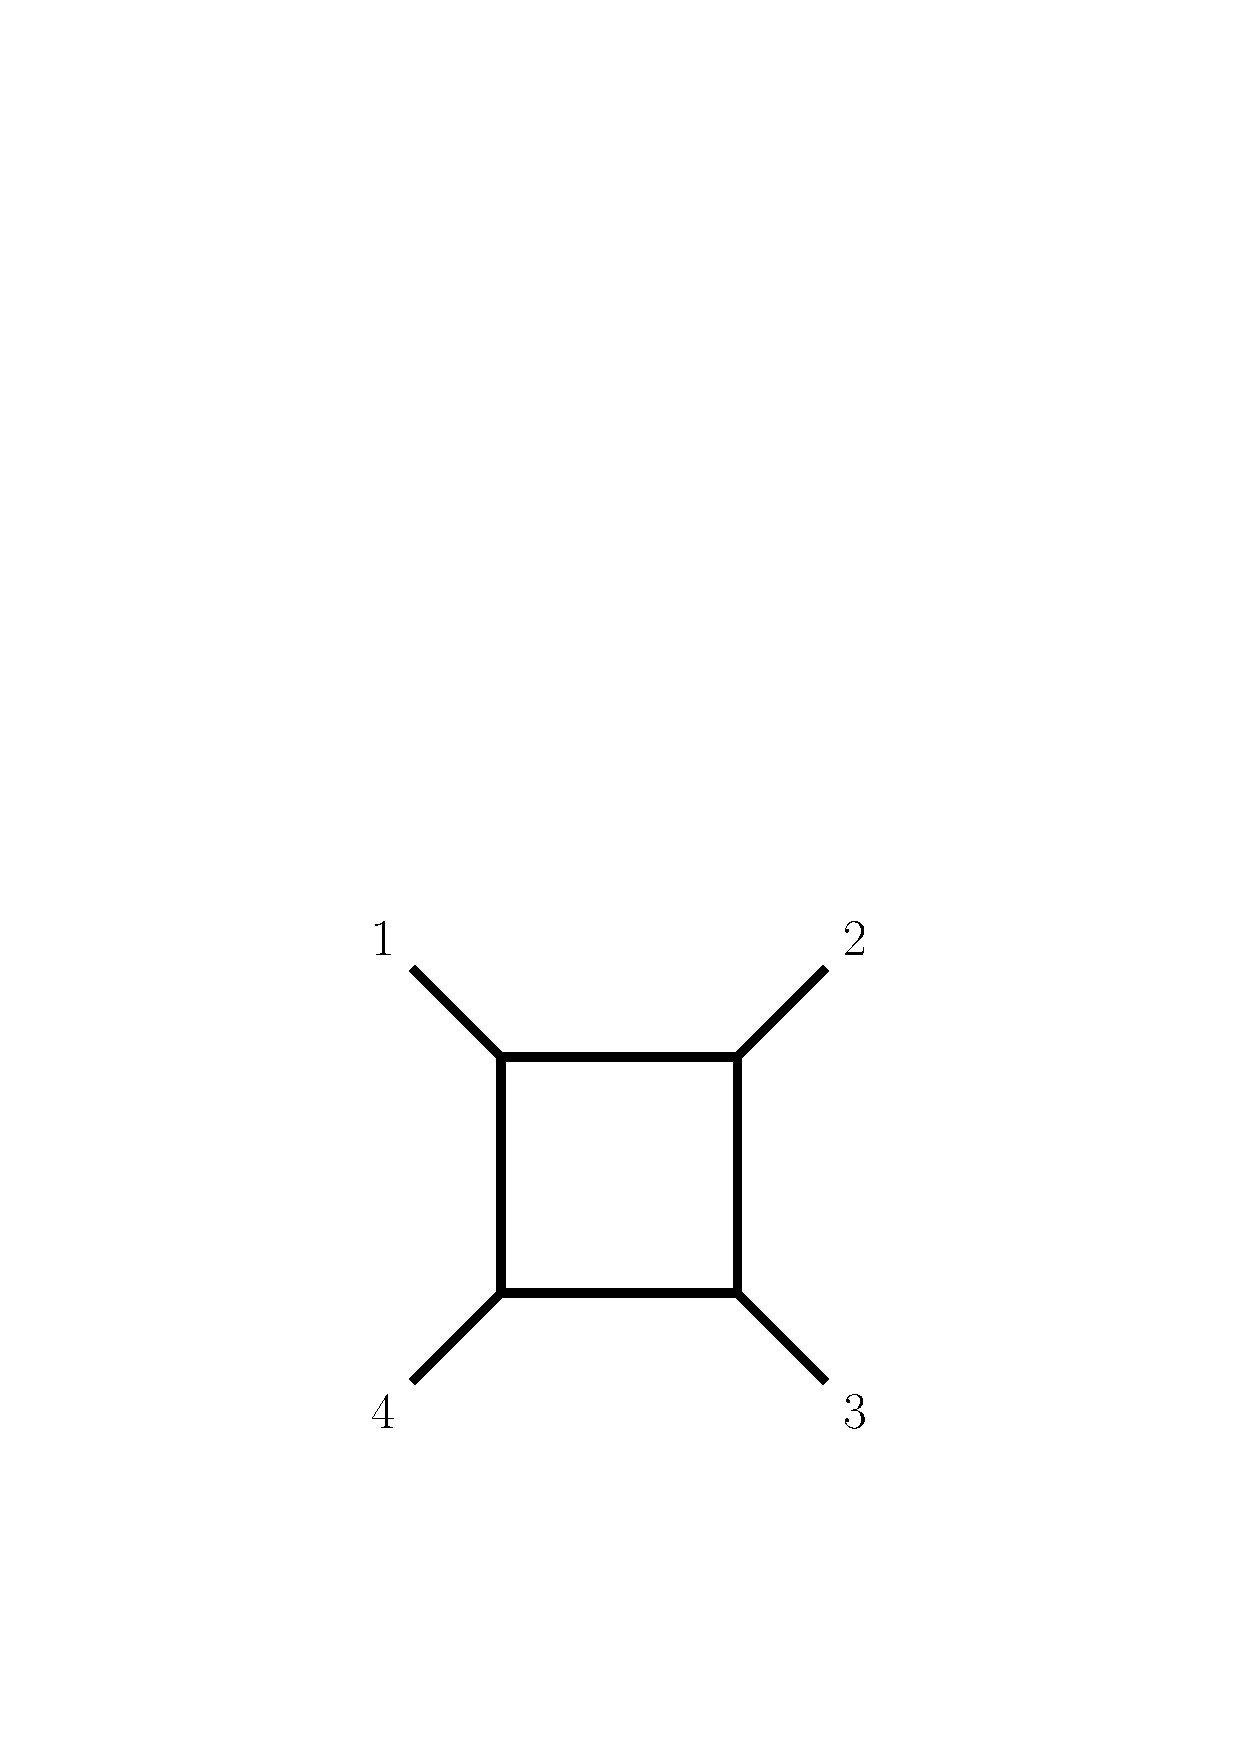
\includegraphics[width=1.8cm]{ch3_loopamps/figures/boxint.pdf}} \right)
  \ = \
  \raisebox{-0.9cm}{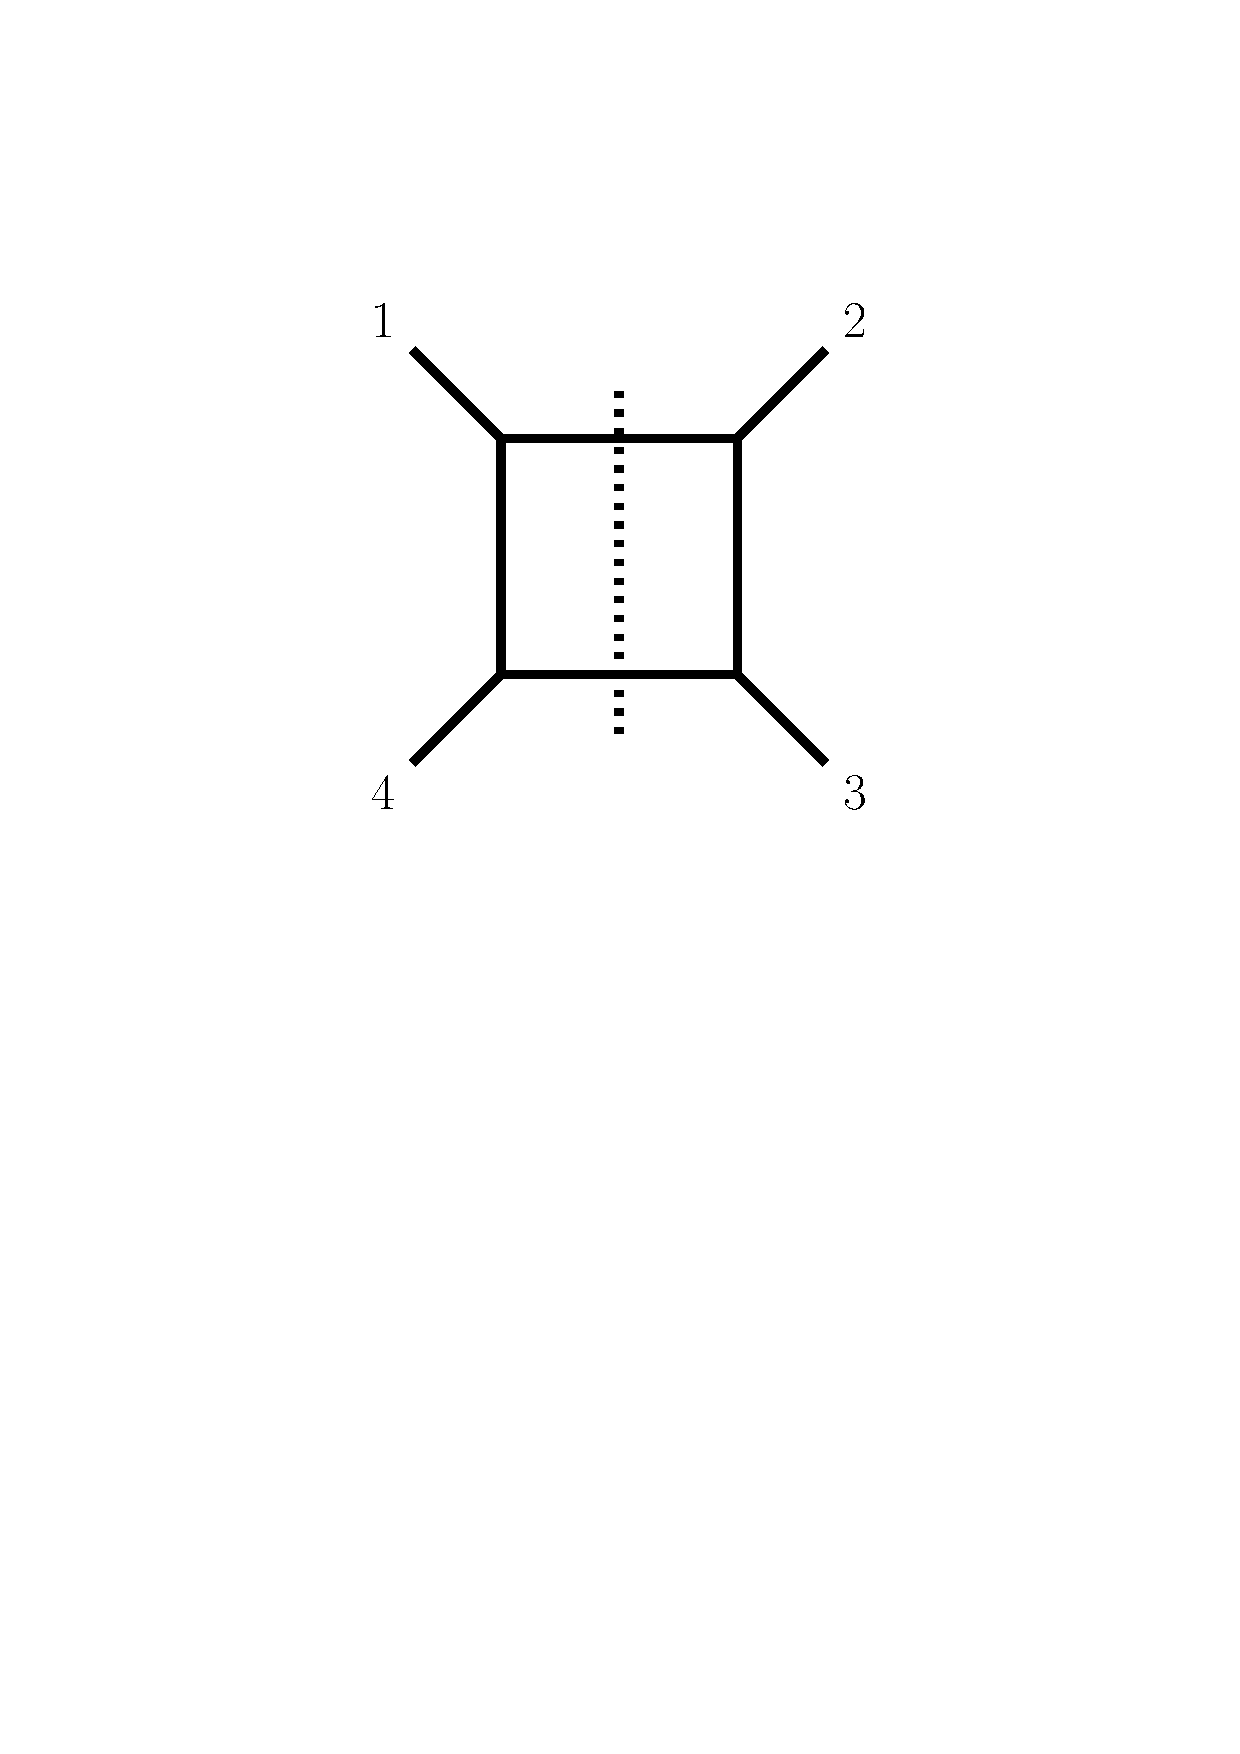
\includegraphics[width=1.8cm]{ch3_loopamps/figures/boxint-tcut.pdf}} \,,
\end{equation}
and so the $s_{23}$-channel cut can be represented as
\begin{align}
    &\mathcal{C}_{23|41} \left(  \raisebox{-0.9cm}{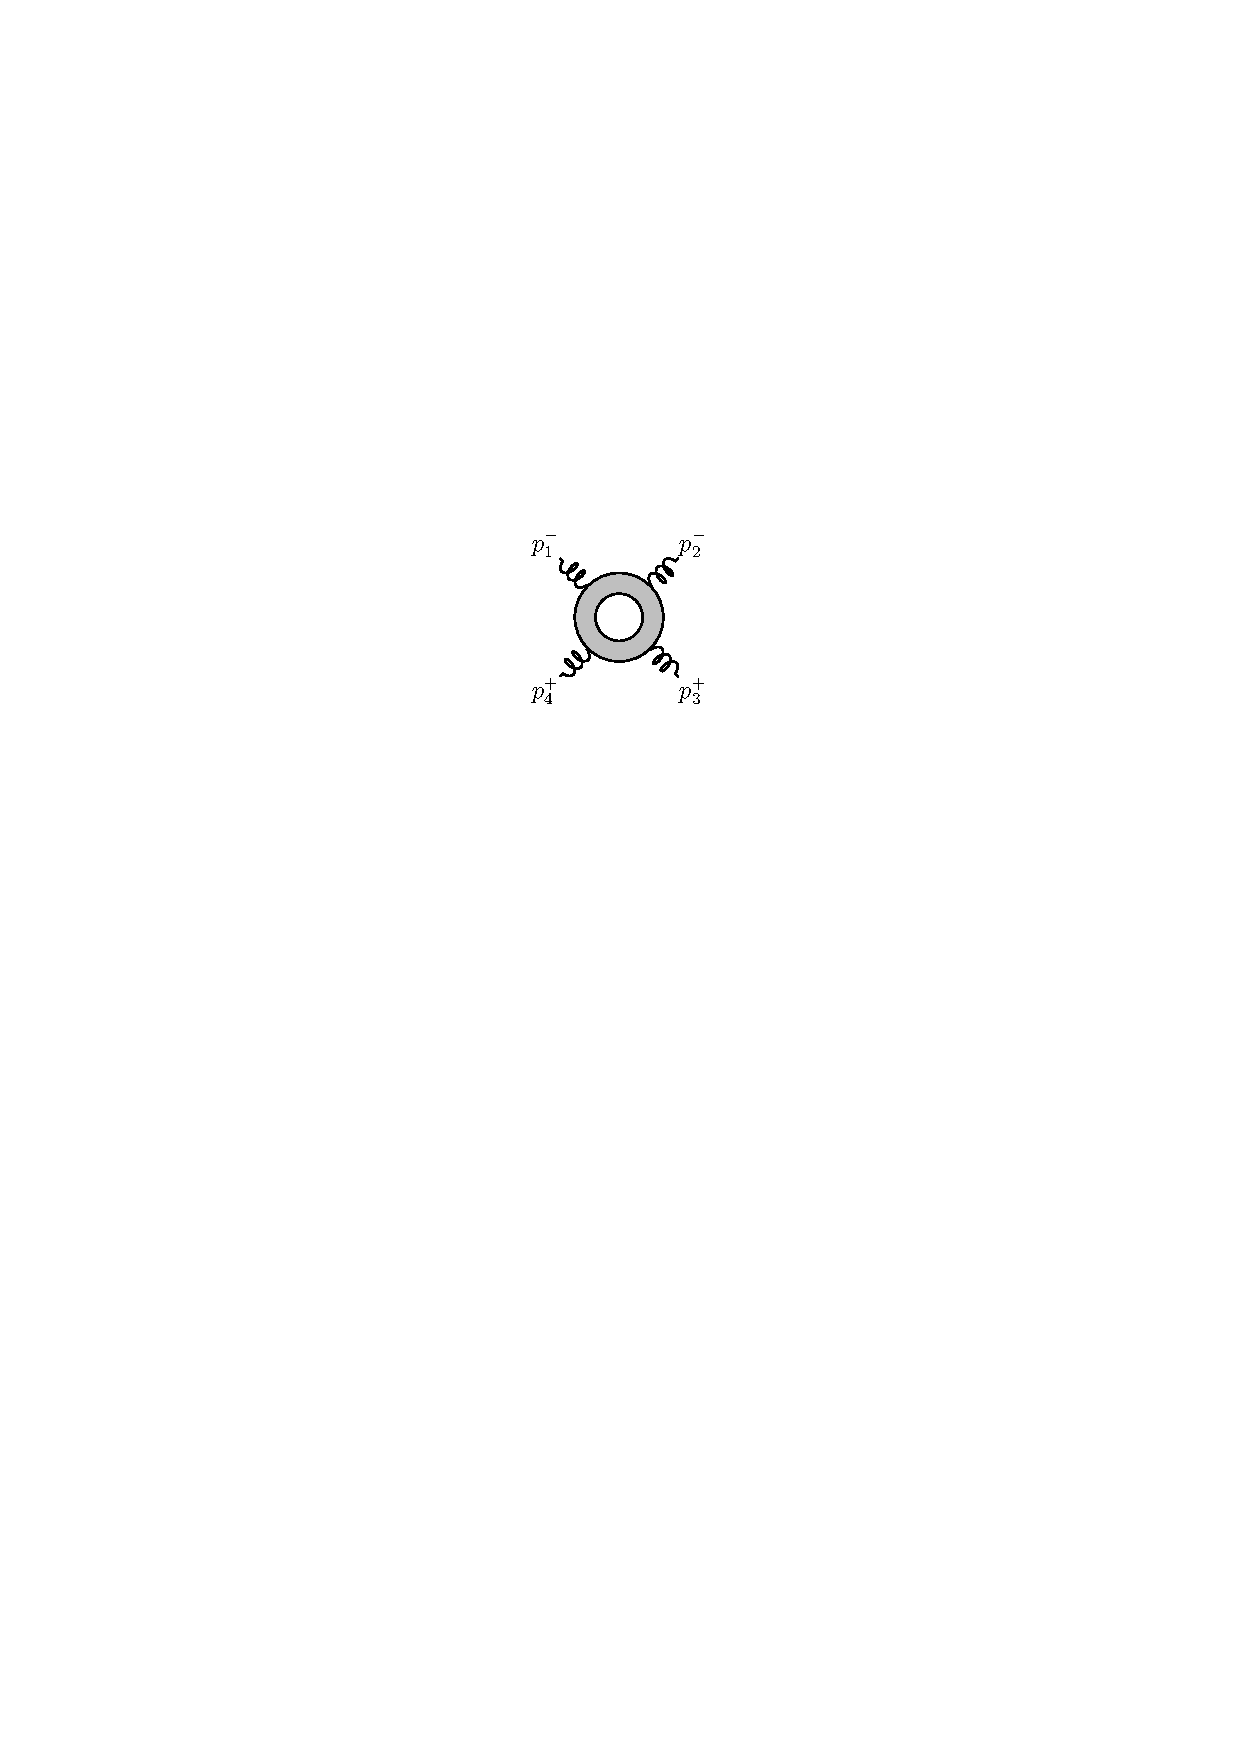
\includegraphics[width=1.8cm]{ch3_loopamps/figures/4g1Lampblob_MHV.pdf}} \right)
    \ = \
    - \raisebox{-0.9cm}{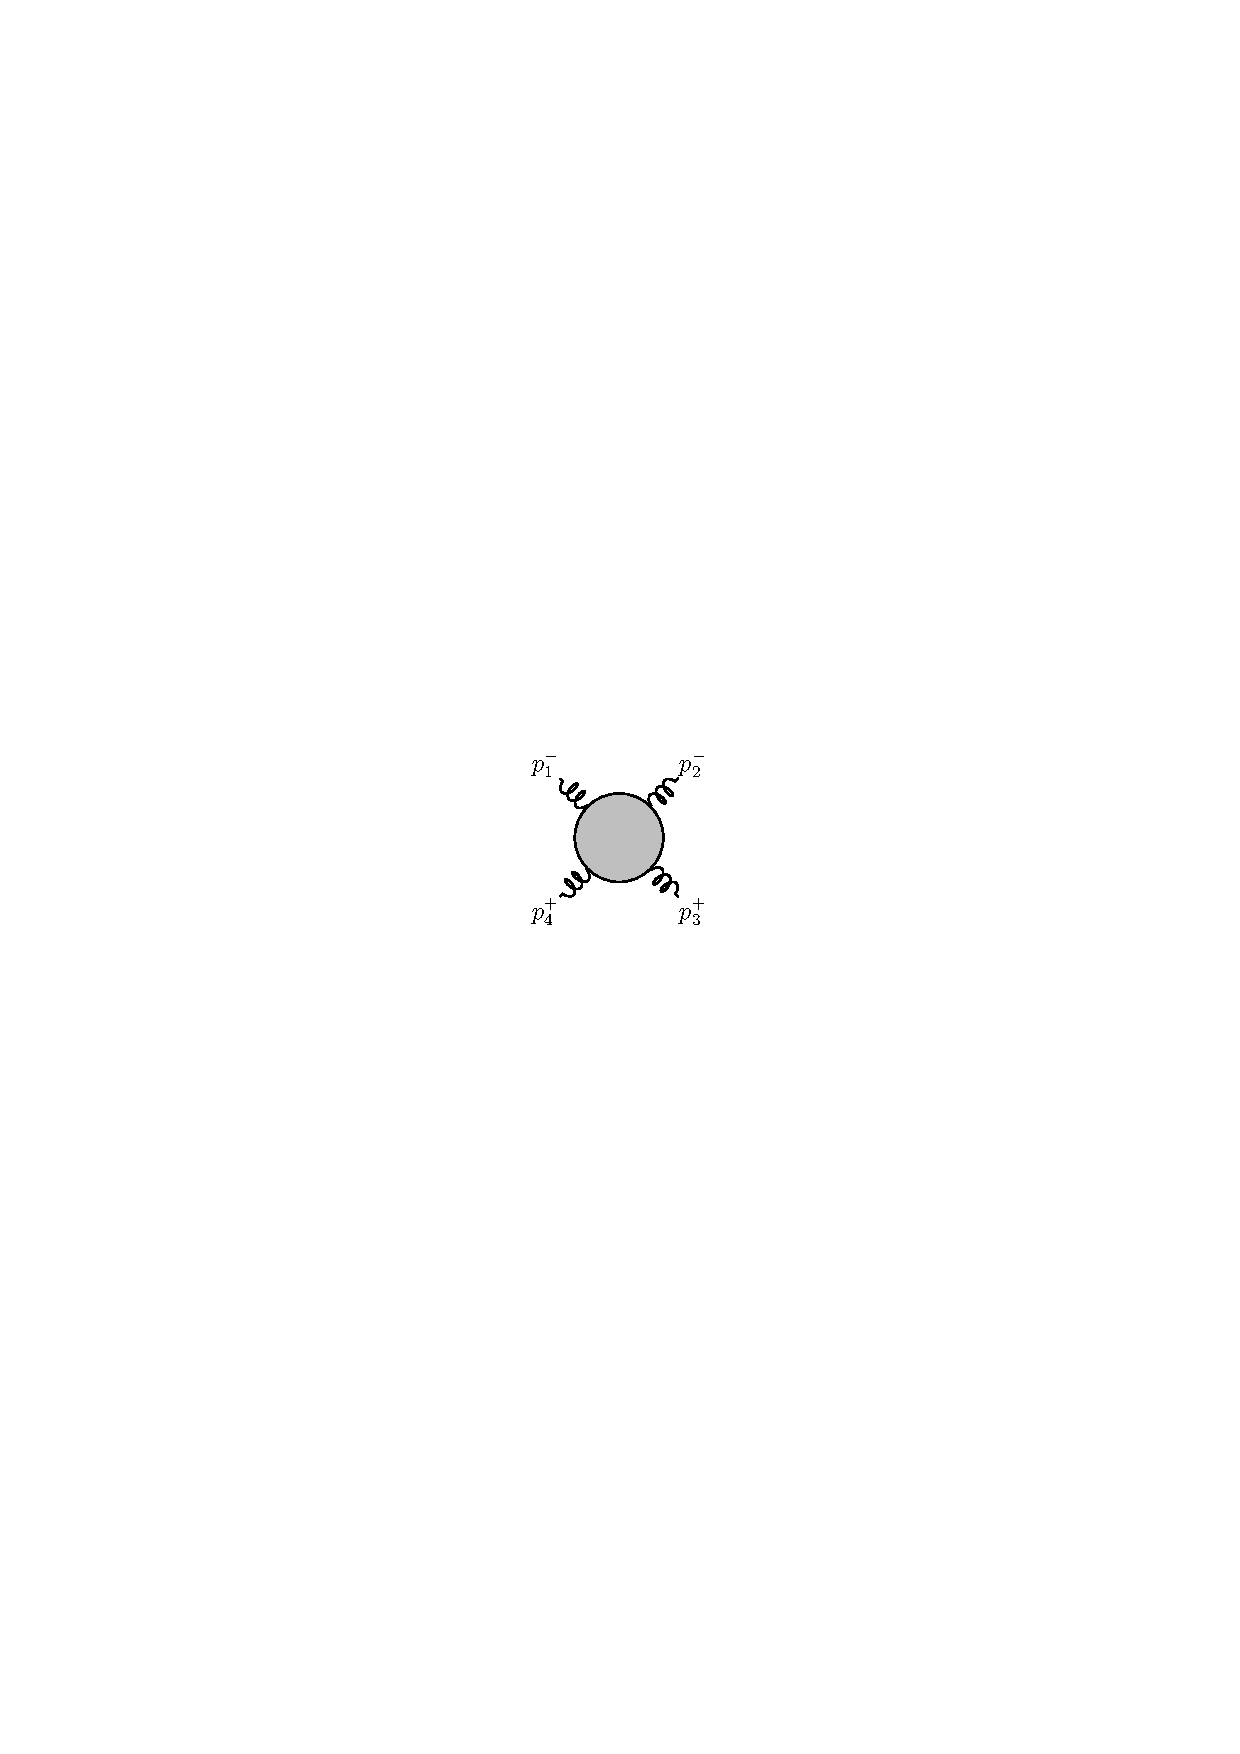
\includegraphics[width=1.8cm]{ch3_loopamps/figures/4g0Lampblob_MHV.pdf}} \left[\rule{0cm}{1cm}\right. 
    s_{12} s_{23} \raisebox{-0.9cm}{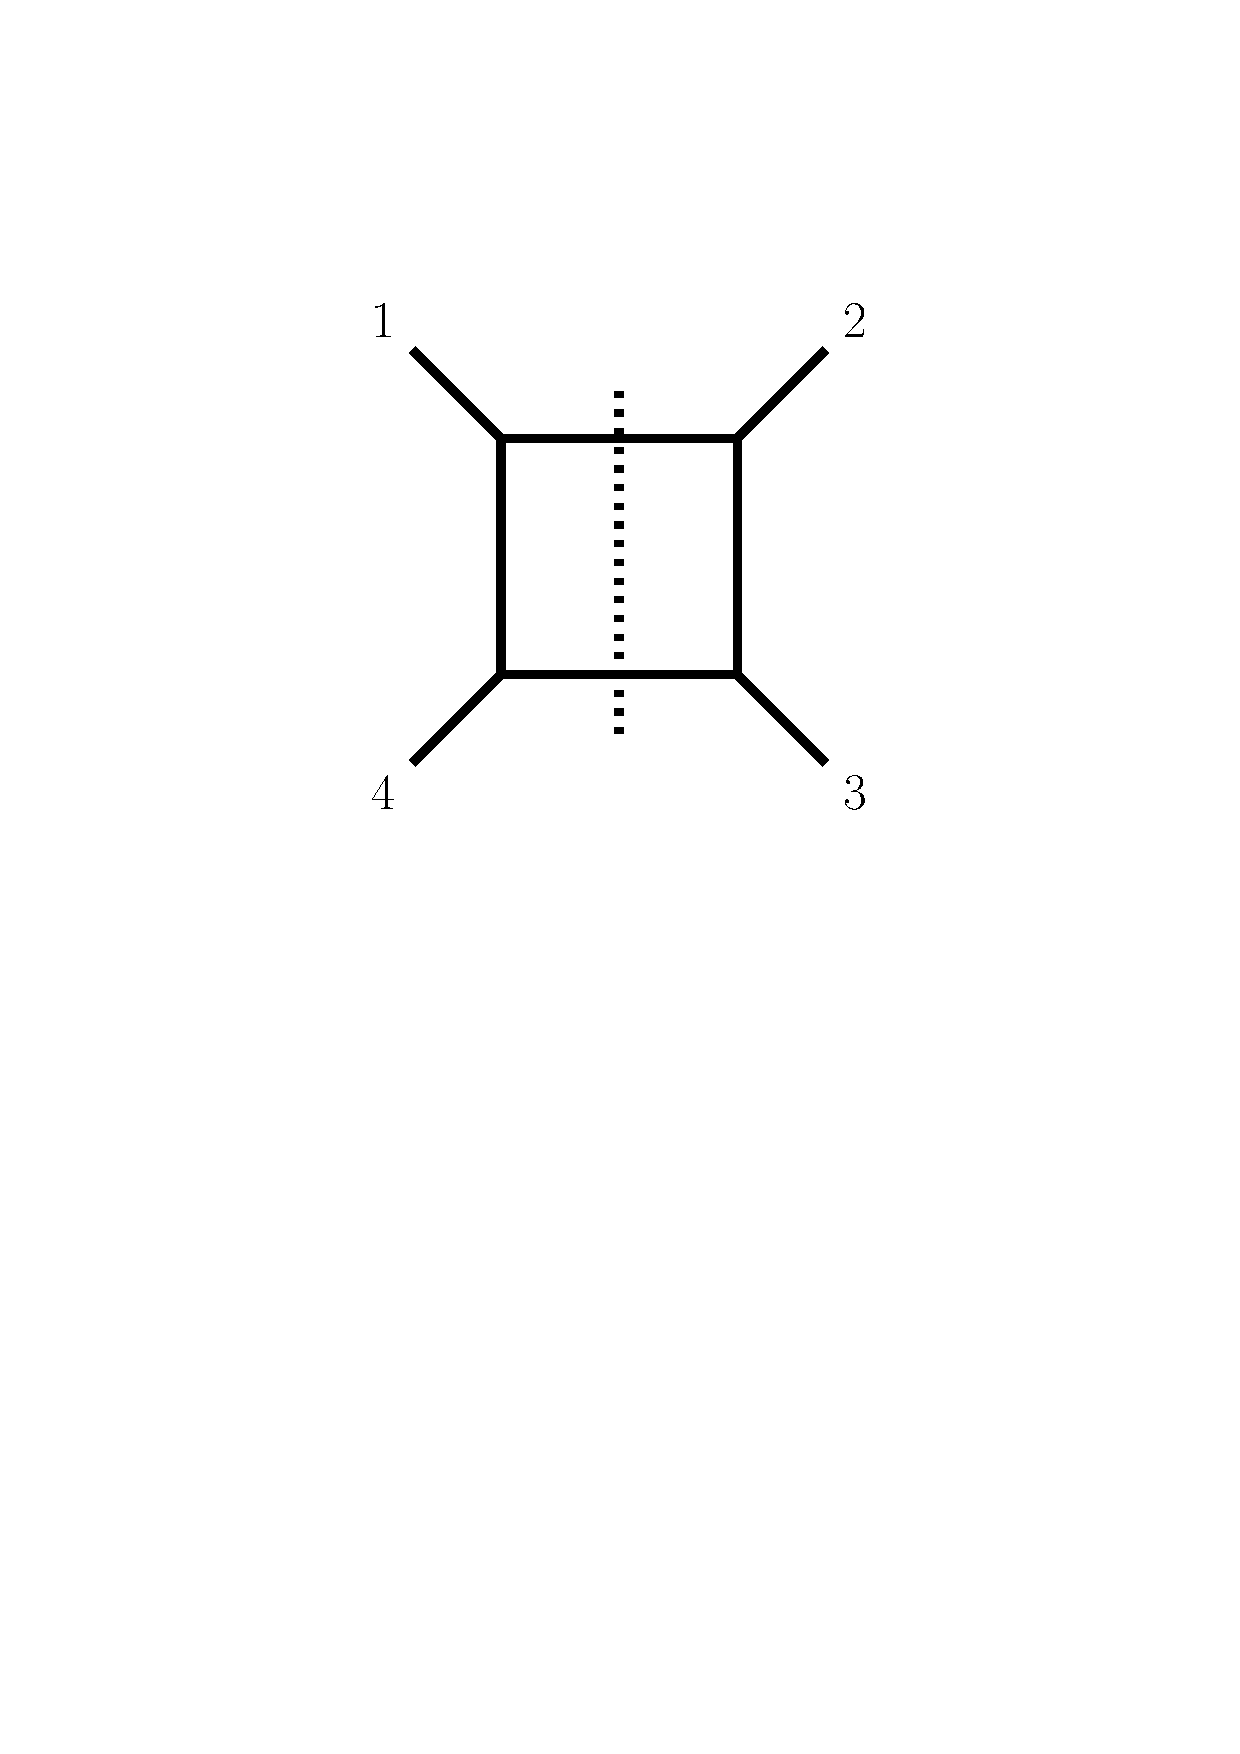
\includegraphics[width=1.8cm]{ch3_loopamps/figures/boxint-tcut.pdf}} \nonumber\\&
    + \frac{2}{s_{12}^2s_{23}^2} \left(
    \raisebox{-0.4cm}{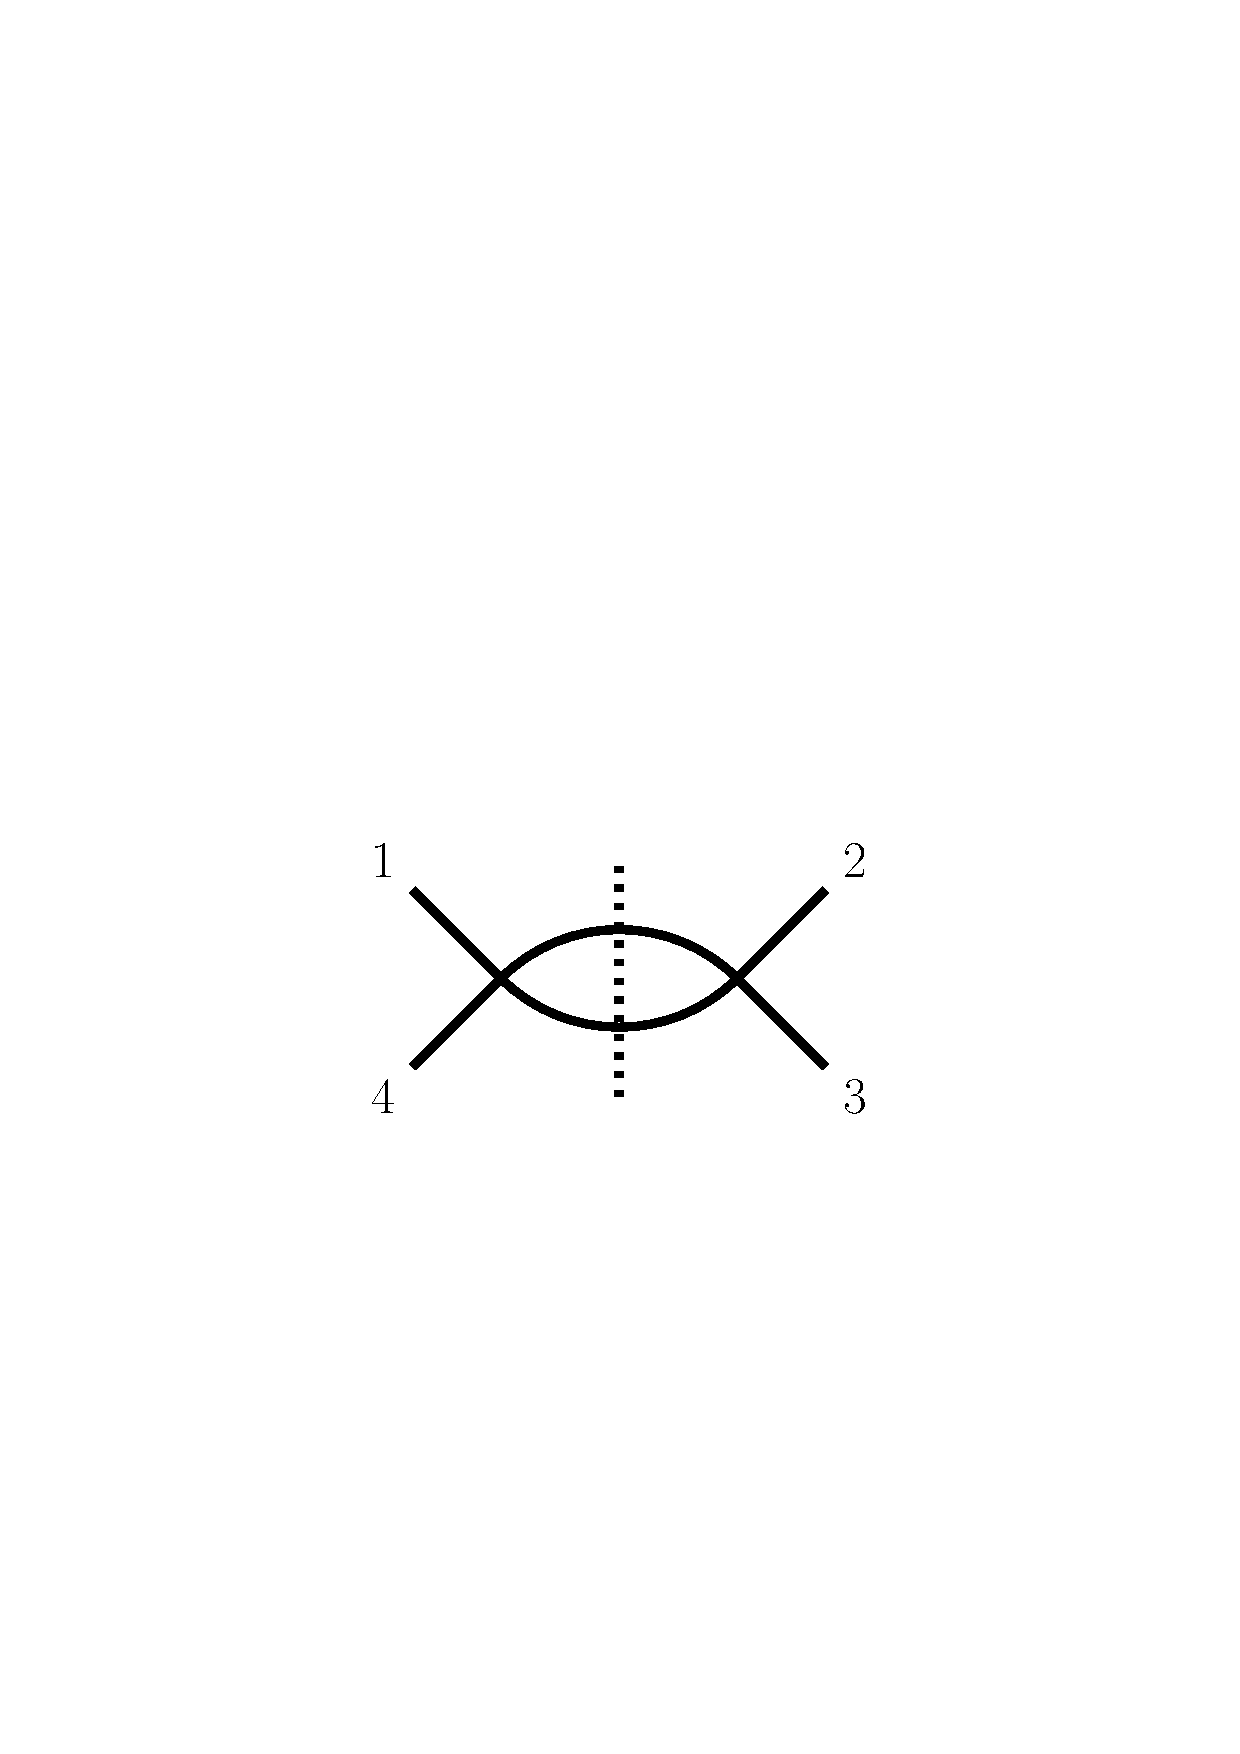
\includegraphics[width=1.8cm]{ch3_loopamps/figures/bub23int_cut23.pdf}}[\mathcal{N}_2]
    + \raisebox{-0.8cm}{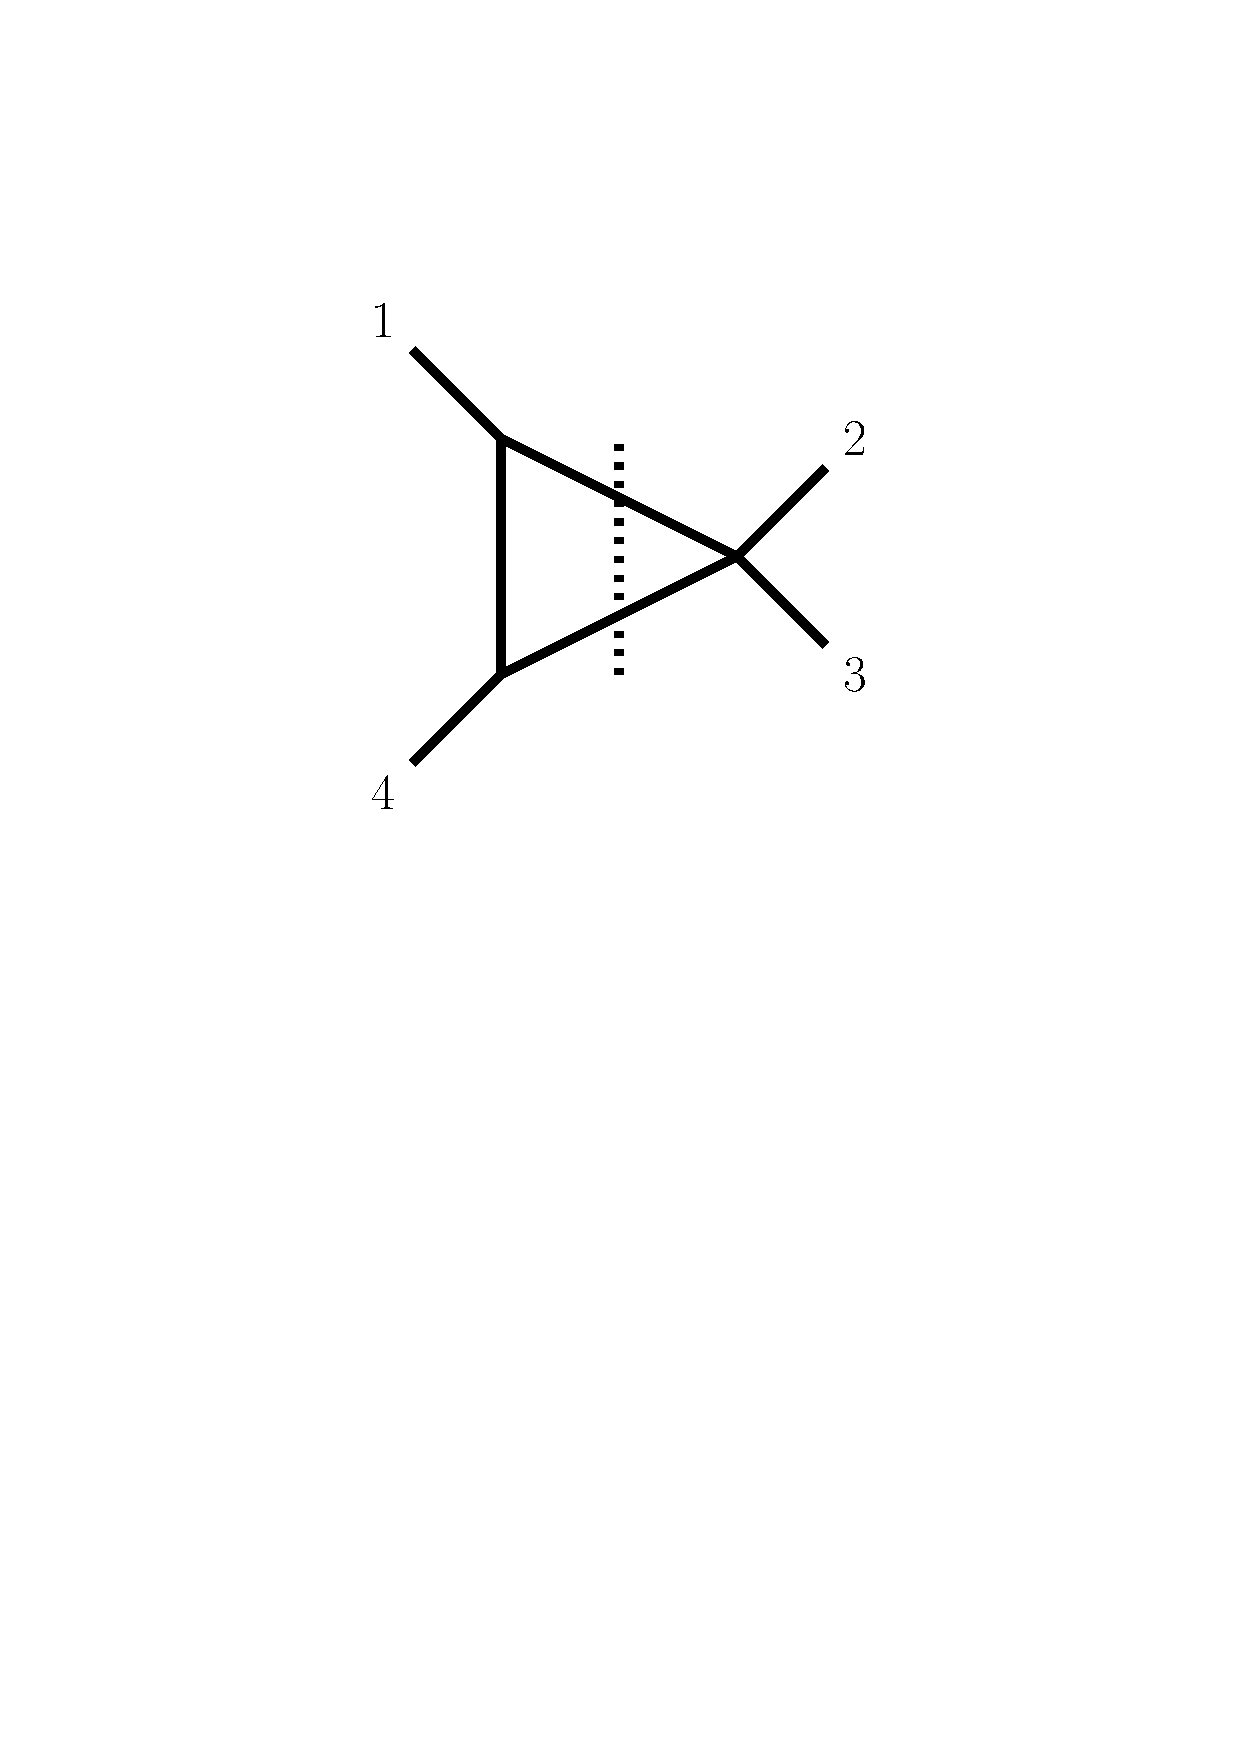
\includegraphics[width=1.8cm]{ch3_loopamps/figures/tri23int_cut23.pdf}}[\mathcal{N}_{3,a}]
    + \raisebox{-0.8cm}{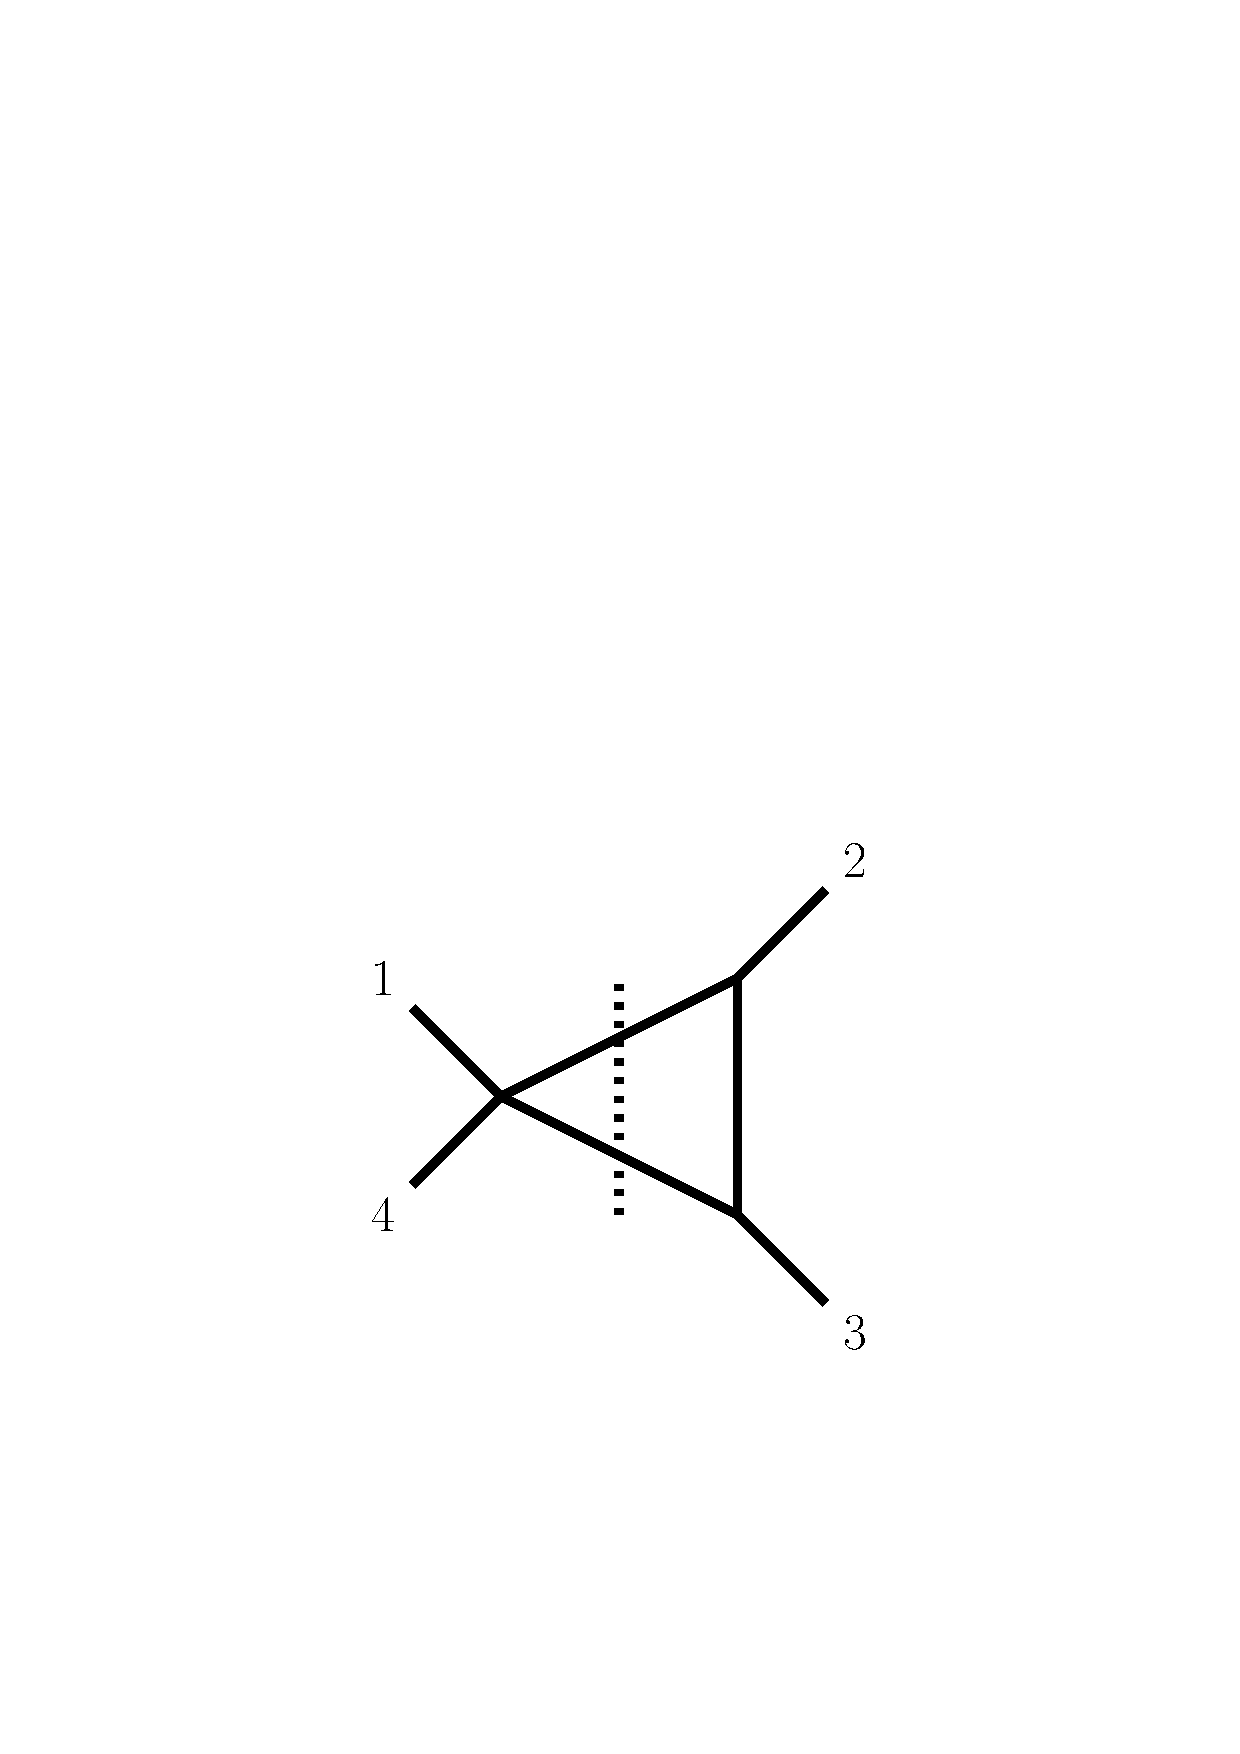
\includegraphics[width=1.8cm]{ch3_loopamps/figures/tri14int_cut23.pdf}}[\mathcal{N}_{3,b}]
    \right)
    \left.\rule{0cm}{1cm}\right] \,.
\end{align}

As we can see, there is still a bit of work to do to simplify this expression. Let us start with the bubble configuration, which has rank-one and and rank-two tensor numerators,
\begin{align} \begin{aligned}
  F_2^{[D]}&(p_{23})[\mathcal{N}_2] = \\
   & \trmgamtwo1{\gamma_{\mu_1}}32 \, \trmgamtwo1{\gamma_{\mu_2}}32 \, F_2^{[D]}(p_{23})\bigl[(k-p_{23})^{\mu_1}(k-p_{23})^{\mu_2}\bigr] \\
  & + s_{12} s_{23} \, \trmgamtwo1{\gamma_{\mu_1}}32 \, F_2^{[D]}(p_{23})\bigl[(k-p_{23})^{\mu_1}\bigr] + 2 \, s_{12}^2s_{23}^2 \, F_2^{[D]}(p_{23})[1] \,.
  \end{aligned}
  \label{eq:c23bubred}
\end{align}
We have already reduced the rank-one integral so we may substitute the form-factor decomposition~\eqref{eq:PVbubR1sol},
\begin{align} \begin{aligned}
  s_{12} s_{23} \, \trmgamtwo{1}{\gamma^{\mu}}{3}{2}
  F_2^{[D]}(p_{23})\bigl[(k-p_{23})^{\mu}\bigr] & = s_{12} s_{23} \left( -\frac{1}{2}\trmgamtwo1{\slashed{p}_{23}}32 \right) F^{[D]}_2(p_{23})[1] \\
  & = -\frac{1}{2} s_{12}^2 s_{23}^2 \, F^{[D]}_2(p_{23})[1] \,.
  \end{aligned}
\end{align}
The rank-two integral will involve several steps of algebra but follows exactly
the same strategy. From \eqn{eq:PVbubR2dec} with the form factors in ~\eqn{eq:rank2bubsol} we may substitute into the
rank-two integral above, obtaining
\begin{align}
  &\trmgamtwo1{\gamma_{\mu_1}}32 \, \trmgamtwo1{\gamma_{\mu_2}}32 \, F_2^{[D]}(p_{23})\bigl[(k-p_{23})^{\mu_1}(k-p_{23})^{\mu_2} \bigr] \nonumber\\
  & \qquad \qquad = a_{2,00} \, \trmgamtwo1{\gamma_{\mu_1}}32 \, \trmgamtwo1{\gamma^{\mu_1}}32 + a_{2,11} \, \trmgamtwo1{\slashed{p}_{23}}32{}^2 \nonumber\\
  & \qquad \qquad = a_{2,11} \, s_{12}^2 s_{23}^2 \nonumber\\
  & \qquad \qquad = \frac{D}{4 (D-1)} F^{[D]}_2(p_{23})[1] \,.
\end{align}
The triangle tensor integrals look troubling at first sight, since we must use reduction for up to rank-three integrals,
\begin{align}
  F^{[D]}_{3}(p_1,p_2)&[k^{\mu_1}] =  a_{3,1} \, p_1^{\mu_1} + a_{3,2} \, p_2^{\mu_1} \,, \label{eq:PVtriR1dec}\\
  F^{[D]}_{3}(p_1,p_2)&[k^{\mu_1}k^{\mu_2}] = \nonumber\\
  & a_{3,00} \, \eta^{\mu_1\mu_2} + a_{2,11} \, p_1^{\mu_1} p_1^{\mu_2}
  + a_{3,12} \left( p_1^{\mu_1} p_2^{\mu_2} + p_1^{\mu_1} p_2^{\mu_2} \right)
  + a_{3,22} \, p_2^{\mu_1} p_2^{\mu_2} \,, \label{eq:PVtriR2dec}\\
  F^{[D]}_{3}(p_1,p_2)&[k^{\mu_1}k^{\mu_2} k^{\mu_3}] = \nonumber\\&
    a_{3,001} \left( \eta^{\mu_1\mu_2} p_1^{\mu_3} + \eta^{\mu_2\mu_3} p_1^{\mu_1} + \eta^{\mu_3\mu_1} p_1^{\mu_2}\right) \nonumber\\&
  + a_{3,002} \left( \eta^{\mu_1\mu_2} p_2^{\mu_3} + \eta^{\mu_2\mu_3} p_2^{\mu_1} + \eta^{\mu_3\mu_1} p_2^{\mu_2}\right) \nonumber\\&
  + a_{3,111} \, p_1^{\mu_1} p_1^{\mu_2} p_1^{\mu_3}
  + a_{3,222} \, p_2^{\mu_1} p_2^{\mu_2} p_2^{\mu_3} \nonumber\\&
  + a_{3,112} \left(p_1^{\mu_1} p_1^{\mu_2} p_2^{\mu_3} + p_1^{\mu_2} p_1^{\mu_3} p_2^{\mu_1} + p_1^{\mu_3} p_1^{\mu_1} p_2^{\mu_2} \right) \nonumber\\&
  + a_{3,122} \left(p_1^{\mu_1} p_2^{\mu_2} p_2^{\mu_3} + p_1^{\mu_2} p_2^{\mu_3} p_2^{\mu_1} + p_1^{\mu_3} p_1^{\mu_2} p_2^{\mu_2} \right) \,.
\label{eq:PVtriR3dec}
\end{align}
Let us start with the easiest rank-one part of the integral $F_3^{[D]}(p_{23},p_{234})$,
\begin{align}
  F_3^{[D]}(p_{23},p_{234})&\bigl[ 2 \, \trmgamtwo1{\slashed{l}_1}42 \, s_{12}^2s_{23}^2 \bigr] \nonumber\\
  &= 2  \, s_{12}^2s_{23}^2 \left( a_{3,1} \, \trmgamtwo1{\slashed{p}_{23}}42 + a_{3,2} \, \trmgamtwo1{\slashed{p}_{234}}42\right) \nonumber\\
 &= 0 \,.
\end{align}
In fact, if we follow through with all the form-factor substitutions we will
see that all tensor triangles reduce to zero. So with a little bit of extra
work with tensor reduction we have found a compact final answer:
\begin{align}
  C'_{23|41} = \ & - 2 \, A^{(0)}(1^-,2^-,3^+,4^+) \frac{1}{s_{12}^2s_{23}^2} \nonumber\\
  & \ \times \mathcal{C}_{23|41}\left(F_2^{[D]}(p_{23})\bigl[\trm\1{l_2}32^2 + s_{12}s_{23} \, \trm1{l_2}32 + 2 \, s_{12}^2s_{23}^2 \bigr]\right)
   \nonumber\\
  = \ & -2 \, A^{(0)}(1^-,2^-,3^+,4^+) \left( \frac{D}{4 (D-1)} -\frac{1}{2} + 2 \right) \mathcal{C}_{23|41}\left(F_2^{[D]}(p_{23})[1]\right) \nonumber\\
  = \ & - A^{(0)}(1^-,2^-,3^+,4^+) \frac{7D-6}{2(D-1)} \, \mathcal{C}_{23|41}\left(F_2^{[D]}(p_{23})[1]\right) \,.
\end{align}
\end{example}

\subsection{Transverse spaces and transverse integration \label{ssec:transverse}}

The development of integrand-reduction techniques led to many efficient
methods for the processing of tensor integrals. Here we would like to
highlight the advantages of decomposing the loop momenta into transverse
components. This feature has been exploited in a number of situations
including---but not exclusively---the loop-momentum basis of Van
Neerven-Vermaseren~\cite{ch3_vanNeerven:1983vr}, Baikov integral
representations~\cite{ch3_Baikov:1996rk},
and the adaptive integrand-reduction method~\cite{ch3_Mastrolia:2016dhn}.

We start by considering an $n$-point, $L$-loop Feynman integral in $D=4-2\eps$
dimensions which depend on $n-1$ independent momenta,
\begin{equation}
  F_n^{(L),[4-2\eps]}(p_1,\cdots,p_{n-1}) = \int_{k_1}\cdots\int_{k_L}  \,f(\{k\}, \{p\}) \,.
\end{equation}
We continue to assume the external momenta $\{p\}$ are in four
dimensions. This implies that the independent external momenta span a space of dimension $m=n-1$ if $n\le 4$, or $m=4$ if $n > 4$. For a one-loop
box integral $m=3$, for a pentagon $m=4$, and a hexagon would also have $m=4$.
So we may write the loop momenta as a decomposition of an $m$-dimensional and
$4-m-2\eps$ dimensional space,
\begin{equation}
  k_i^\mu = k_i^{\mu,[m]} + k_i^{\mu,[4-2\eps-m]} \,,
\end{equation}
which are orthogonal, 
\begin{equation}
  k_i^{\mu,[m]}\cdot k_j^{\mu,[4-m-2\eps]} = 0 \,.
\end{equation}
If $m<4$ (i.e., if $n \le 4$), we may even consider three transverse spaces of dimensions $m$, $4-m$ and $-2\eps$,
\begin{equation}
  k_i^\mu = k_i^{\mu,[m]} + k_i^{\mu,[4-m]} + k_i^{\mu,[-2\eps]} \,,
\end{equation}
all orthogonal to each other.
Since the various indices become cumbersome at this point it is convenient to introduce some notation:
\begin{align*}
  &k_i^{\mu,[m]} = k^\mu_{i,\parallel} \text{ spans the physical space of the loop integral},\\
  &k_i^{\mu,[4-m]} = k^\mu_{i,\perp} \text{ spans the spurious space of the loop integral},\\
  &k_i^{\mu,[-2\eps]} \text{ spans the extra-dimensional space of the loop integral},\\
  &k_i^{\mu,[4-m-2\eps]} \text{ spans both spurious and extra-dimensional space of the loop integral}.
\end{align*}
We use the term \textit{physical} to indicate the space after integration, i.e.\
the space of independent external momenta that we used for tensor reduction in section~\ref{sec:3.4}.
The term \textit{spurious} space is used to indicate terms that are non-zero at
the level of the integrand but which will vanish after integration.
For each of these spaces a spanning set of momenta can be found. The construction
of such a basis is often referred to as the Van Neerven-Vermaseren
basis~\cite{ch3_vanNeerven:1983vr}. For the physical space $k^\mu_{i,\parallel}$ the
\textit{independent} external momenta can be used. For the spurious space $k^\mu_{i,\perp}$ we may find an orthogonal basis of
four-dimensional vectors. Traditionally these are denoted $\omega_i^\mu$ and depend on the vectors $p_i^\mu$ spanning the physical space.
In the Van Neerven-Vermaseren construction they are orthonormal, i.e.\ $\omega_i\cdot \omega_j = N_i \delta_{ij}$ with $N_i=1$.
In a given implementation it can be beneficial to let $N_i \neq 1$ in order to
avoid square roots in the kinematic invariants.

Let us give an explicit example to make things clearer. Consider a one-loop
triangle configuration with massless external momenta $p_1, p_2$ and $p_3$.
This means the spurious space has dimension two and the physical space may be
spanned by $\{p_1, p_2\}$. General four-dimensional vectors may be written as
\begin{equation}
  \omega_i^\mu(p_1,p_2) = \alpha_{1i} \, p_1^\mu + \alpha_{2i} \, p_2^\mu + \alpha_{3i} \, \frac{1}{2} \spAB{1}{\gamma^\mu 2 X}{1} + \alpha_{4i} \, \frac{1}{2} \spAB{2}{\gamma^\mu 1 X}{2} \,,
  \label{eq:spuriousvectorexampeEQ1}
\end{equation}
where $i=1,2$, and we have introduced an arbitrary reference momentum $X$ to ensure the coefficients $\alpha$ are free of any spinor phase.

The spurious vectors satisfy the conditions $\omega_i\cdot p_j = 0$ and $\omega_i\cdot \omega_j = \delta_{ij}$ if
\begin{align}
  \alpha_{1i} = \alpha_{2i} = 0 \,, \qquad
  \alpha_{31}\alpha_{42} + \alpha_{41}\alpha_{32} = 0 \,, \qquad
  - \frac{1}{2} s_{12} {\rm tr}(\slashed1 \slashed{X} \slashed2 \slashed{X}) \alpha_{3i} \alpha_{4i} = 1 \,,
  \label{eq:spuriousvectorexampeEQ2}
\end{align}
for $i=1,2$, and so we find the explicit representation
\begin{align} \label{eq:triangle_omegas}
\begin{aligned}
  \omega_1^\mu(p_1,p_2) &= \frac{\sqrt{2}}{\sqrt{s_{12}{\rm tr}_(\slashed1 \slashed{X} \slashed2 \slashed{X})}}\bigl(\spAB{1}{\gamma^\mu 2 X}{1}  - \spAB{2}{\gamma^\mu 1 X }{2}\bigr) \,, \\
  \omega_2^\mu(p_1,p_2) &= \frac{\i\sqrt{2}}{\sqrt{s_{12}{\rm tr}(\slashed1 \slashed{X} \slashed2 \slashed{X})}}\bigl(\spAB{1}{\gamma^\mu 2 X}{1}  + \spAB{2}{\gamma^\mu 1 X}{2}\bigr) \,.
\end{aligned} 
\end{align}
In the context of a full amplitude computation, the momentum $X$ could be one
of the other independent external momenta. It is also clear in this expression that
the complicated prefactor results from the assertion that the vectors should be
orthonormal, and can be avoided by releasing the condition without affecting any
final amplitude level results. Numerators for amplitudes in the transverse
space (which are Lorentz scalars) may now be expressed in terms of scalar
products $k_1\cdot \omega_i$,
\begin{equation}
  k^\mu_{1,\perp} =  (k_1\cdot \omega_1) \, \omega_1^\mu + (k_1\cdot \omega_2) \, \omega_2^\mu \,.
\end{equation}

We could try to span the extra-dimensional space with explicit vectors, though
we would be forced to introduce a fixed embedding dimension larger than four to
do it. As a result we would lose all the convenient four-dimensional spinor-helicity methods
that have been working well so far. Instead, we simply identify the independent
scalar products appearing, which depend only on the number of loops. At one-loop
there would only be a single extra-dimensional scalar product,
\begin{equation}
  k_1^{[-2\eps]}\cdot k_1^{[-2\eps]} \eqqcolon -\mu_{11}\,.
  \label{eq:extradimSP1}
\end{equation}
The definition of the extra-dimensional scalar product $\mu_{11}$
includes a sign so this appears as an effective mass term in the
propagator,
\begin{equation}
  k_1^2 = k_{1,\parallel}^2 + k_{1,\perp}^2 - \mu_{11}\,.
\end{equation}
At higher loops more extra-dimensional scales will be introduced, which may be
labelled $\mu_{ij} \coloneqq - k_i^{[-2\eps]} \cdot k_j^{[-2\eps]}$. At
two-loops there would be three such scales and $L(L+1)/2$ for the general $L$-loop case.

We finish this section by demonstrating a useful application of the
decomposition into transverse spaces: \emph{transverse integration}. If the numerator
for a given tensor integral lives in a transverse space, we may provide a
general tensor decomposition using only the metric tensor in the transverse
space. For example, returning to the one-loop triangle, consider:
\begin{align}
  \int_k \frac{k\cdot\omega_i}{k^2 (k-p_1)^2 (k-p_{12})^2}  
  &= \omega_{i,\mu} \int_k \frac{k^\mu}{k^2 (k-p_1)^2 (k-p_{12})^2} \nonumber \\
    &= \omega_{i,\mu}  \left(a_{3,1} \, p_1^\mu + a_{3,2} \, p_2^{\mu}\right) \nonumber \\
    & = 0\,,
\end{align}
where we have used the Passarino-Veltman reduction from the previous section.
Following the same logic it should be clear that for any odd power, $r$, of the
numerator $(k\cdot\omega_i)^r$, the integral will vanish. Even powers do not
vanish, but we may expand the tensor integral using the metric tensor
$\eta^{\mu\nu, [m]}$ for $m=2$, which satisfies
\begin{equation}
  \eta_{\ \ \mu}^{\mu, [m]} = m\,.
\end{equation}
The tensor decomposition can be written in terms of a form factor
$\tilde{a}_{3,00}^{[2]}$ which multiplies the metric tensor of the two-dimensional
spurious space. For instance, for $r=2$, we have that
\begin{align}
  \int_k \frac{(k\cdot \omega_i)^2}{k^2 (k-p_1)^2 (k-p_{12})^2} 
  &= \omega_{i,\mu_1} \, \omega_{i,\mu_2} \int_k \frac{k_\perp^{\mu_1} k_\perp^{\mu_2}}{k^2 (k-p_1)^2 (k-p_{12})^2} \nonumber\\
  &= \omega_{i,\mu_1} \, \omega_{i,\mu_2} \, \tilde{a}_{3,00}^{[2]} \, \eta^{\mu_1\mu_2, [2]} \nonumber\\
  &= \omega_i^2 \, \tilde{a}_{3,00}^{[2]} \,.
  \label{eq:triwsqtransverseint}
\end{align}
Projecting using the tensor $\eta_{\mu_1\mu_2}^{[2]}$ leads to
\begin{align}
  \tilde{a}_{3,00}^{[2]} \, \eta^{\mu_1\mu_2, [2]} \, \eta_{\mu_1\mu_2}^{[2]} &= 2 \, \tilde{a}_{3,00}^{[2]} \\
   &= \int_k \frac{k_\perp^2}{k^2 (k-p_1)^2 (k-p_{12})^2} \\
   &= \int_k \frac{k^2-k_{\parallel}^2+\mu_{11}}{k^2 (k-p_1)^2 (k-p_{12})^2}\,.
\end{align}
The term $k_{\parallel}^2$ may be written in terms of the propagators by decomposing $k^{\mu}_{\parallel}$ as
\begin{align}
k_{\parallel}^\mu = \frac{k_{\parallel}\cdot p_2}{p_1\cdot p_2} \, p_1^\mu + \frac{k_{\parallel}\cdot p_1}{p_1\cdot p_2} \, p_2^\mu \,.
\end{align}
This in fact implies that 
\begin{align}
   k_{\parallel}^2 = \frac{2 \, (k_{\parallel}\cdot p_1) (k_{\parallel}\cdot p_2)}{p_1\cdot p_2}\,,
\end{align}
which can be expressed in terms of the propagators using
\begin{align}
  2 \, k_{\parallel}\cdot p_1 &= k^2 - (k-p_1)^2 \,, \\
  2 \, k_{\parallel}\cdot p_2 &= (k-p_1)^2 - (k-p_{12})^2 + s_{12} \,.
\end{align}
In this way we write the original rank-two tensor integrals in terms of the
usual Feynman integrals but including a triangle with $\mu_{11}$ in the
numerator. We will see later that there are methods to integrate it directly.
We may also observe a very similar but alternative derivation of the same integral:
\begin{align}
  \int_k \frac{(k\cdot\omega_i)^2}{k^2 (k-p_1)^2 (k-p_{12})^2} 
  &= \omega_{i,\mu_1} \omega_{i,\mu_2} \int_k \frac{k_\perp^{\mu_1} k_\perp^{\mu_2}}{k^2 (k-p_1)^2 (k-p_{12})^2} \\
  &= \omega_{i,\mu_1} \omega_{i,\mu_2} \int_k \frac{k^{\mu_1, [2-2\eps]} k^{\mu_2, [2-2\eps]}}{k^2 (k-p_1)^2 (k-p_{12})^2} \\
  &= \omega_{i,\mu_1} \omega_{i,\mu_2} \, \tilde{a}^{[2-2\eps]}_{3,00} \, \eta^{\mu_1\mu_2, [2-2\eps]}\,.
\end{align}
This time the form factor $\tilde{a}^{[2-2\eps]}_{3,00}$ multiplies the metric
tensor of the $(2-2\eps)$-dimensional spurious and extra-dimensional spaces. Contracting this expression with the same metric tensor gives
\begin{align}
\begin{aligned}
   \tilde{a}^{[2-2\eps]}_{3,00} \, \eta^{\mu_1\mu_2, [2-2\eps]} \, \eta_{\mu_1\mu_2}^{[2-2\eps]} &= 2(1-\eps) \, \tilde{a}^{[2-2\eps]}_{3,00} \\
   &= \int_k \frac{k^2-k_{\parallel}^2}{k^2 (k-p_1)^2 (k-p_{12})^2}\,,
 \end{aligned}
\end{align}
which does not include the $\mu_{11}$ integral. We recall that $k_{\parallel}^2$ can be written in terms of propagators as discussed above. Putting everything together we obtain
\begin{align}
\begin{aligned}
\int_k \frac{(k\cdot\omega_i)^2}{k^2 (k-p_1)^2 (k-p_{12})^2}
&= \omega_{i}^2 \, \frac{1}{2} \int_k \frac{k^2-k_{\parallel}^2+\mu_{11}}{k^2 (k-p_1)^2 (k-p_{12})^2} \\
&= \omega_{i}^2 \, \frac{1}{2(1-\eps)} \int_k \frac{k^2-k_{\parallel}^2}{k^2 (k-p_1)^2 (k-p_{12})^2}\,.
\end{aligned}
\end{align}
Comparing both results we find that
\begin{equation}
  \int_k \frac{\mu_{11}}{k^2 (k-p_1)^2 (k-p_{12})^2} = -\frac{\eps}{1-\eps} \int_k \frac{k^2-k_{\parallel}^2}{k^2 (k-p_1)^2 (k-p_{12})^2}\,.
  \label{eq:mu11triformula}
\end{equation}
This exercise demonstrates a number of ways to move around the space of loop
integrals and integrands, and gives us enough technology to describe a complete
procedure for the computation of one-loop amplitudes.


\begin{exer}{Spurious loop-momentum space for the box integral}
\label{Ex:3.4}
Consider a one-loop box configuration with massless external momenta $p_1$, $p_2$, $p_3$, and $p_4$ ($p_i^2 = 0$, $p_1+p_2+p_3+p_4=0$). 

\begin{enumerate}[a)]
\item Determine the dimension of the physical and of the spurious space. Construct a basis of the latter using the spinors associated with the external momenta.
\smallskip
\item Show that the vector spanning the spurious space is proportional to
\begin{align} \label{eq:omega4pt}
\omega^{\mu}(p_1,p_2,p_3) = \epsilon^{\mu \nu \rho \sigma} p_{1\mu} p_{2\rho} p_{3\sigma} \,. 
\end{align}
\end{enumerate}
\noindent
Note that $\omega^{\mu}$ in \eqn{eq:omega4pt} spans the one-loop box spurious space also for massive or off-shell external momenta ($p_i^2 \neq 0$). In other words, $\omega(p_1,p_2,p_3) \cdot p_i = 0$ for any $i=1,\ldots,4$.
For the solution see \hyperref[Sol:3.4]{chapter~5}.
\end{exer}


\section{General integral and integrand bases for one-loop amplitudes \label{sec:3.5}}

\subsection{The one-loop integral basis}

At the beginning of this chapter we already introduced the idea that any
loop amplitude may be decomposed into an analytic part (a Feynman integral) and
an algebraic (or rational) coefficient. Using our notation for one-loop amplitudes (while continuing to suppress couplings, $\mu_{\rm R}$ and $4\pi$ prefactors) this reads
\begin{align}
  A_n^{(1),[D]}(1,\ldots,n) =
  \sum_{m,N} \i \, c_{m,N}^{[D]} (1,\cdots,n) \, F_{m}^{[D]}(p_1,\cdots,p_{n-1})[N] \,,
  \label{eq:loopamp-general-repeat}
\end{align}
where we must finalise the sum of propagator multiplicity $m$ and numerators
$N$ which form an integral basis.  In the examples of tensor integral reduction
we have seen how the large numbers of tensor integrals which appear in the
amplitude can be reduced onto a small number of integrals resulting in large
simplifications. If we collect the results from sections~\ref{sec:3.2} and~\ref{sec:3.4} we can summarise the information we have gathered about the four-gluon MHV amplitude in $D=4-2\eps$ dimensions as
\begin{align}
  A^{(1),[4-2\eps]}(1^-,&2^-,3^+,4^+) = A^{(0)}(1^-,2^-,3^+,4^+) \nonumber\\&
     \times \bigg(-s_{12}s_{23} F^{[4-2\eps]}_4(p_{1},p_{2},p_{3})[1] - \frac{11}{3} F^{[4-2\eps]}_2(p_{23})[1] \bigg)
     \nonumber\\&
     + \text{terms missed in 4D} \,.
   \label{eq:4g1loop}
\end{align} 
Here we have used the notation from section~\ref{sec:3.4}, where the integrals
are labelled by the external momenta flowing in the propagators and the
numerator dependence, in both cases here just simple scalar integrals.

At one loop the tensor-reduction method is sufficient to completely classify the
basis of all one-loop integrals for an arbitrary number of external momenta
with arbitrary kinematics. In order for it to be clear where we are going as we
derive this basis, let us begin by quoting the final result.

\begin{important}{A general formula for one-loop amplitudes}
A one-loop amplitude in dimensional regularisation with four-dimensional external states can be written as
\begin{align}
  A^{(1),[4-2\eps]}_n&(1,\ldots,n) = \nonumber\\&
    \sum_{1\leq i_1<i_2<i_3<i_4\leq n} \i \, c_{0;i_1|i_2|i_3|i_4} \, F^{[4-2\eps]}_4(p_{i_1,i_2-1},p_{i_2,i_3-1},p_{i_3,i_4-1})[1]\nonumber\\&
  + \sum_{1\leq i_1<i_2<i_3\leq n} \i \, c_{0;i_1|i_2|i_3} \, F^{[4-2\eps]}_3(p_{i_1,i_2-1},p_{i_2,i_3-1})[1]\nonumber\\&
  + \sum_{1\leq i_1<i_2\leq n} \i \, c_{0;i_1|i_2} \, F^{[4-2\eps]}_2(p_{i_1,i_2-1})[1]\nonumber\\&
  + \sum_{1\leq i_1\leq n} \i \, c_{0;i_1} F^{[4-2\eps]}_1(p_{i_1})[1]\nonumber\\&
  + R(1,\ldots,n) + \mathcal{O}(\eps) \,,
  \label{eq:oneloop4dbasis}  
\end{align}
where $R$ is a rational function of the external kinematics. There is quite a
lot going on here so let us unpack it. Firstly we see that result is quoted
in $4-2\eps$ dimensions and given only up to terms of $\mathcal{O}(\eps^0)$. No
integral functions with more than four propagators are required and only scalar
numerators appear. The rational coefficients, $c$, do not depend on $\eps$ and
may be obtained using four-dimensional unitarity cuts. The only term missed by
the four-dimensional cuts is a rational term. We will need to work a little
harder before we can justify that the remaining contribution is simply a
rational function, and for now we leave it as statement without proof. Let us also
clarify that the term \textit{rational function of the external kinematics} is
used to indicate a rational function of spinor products and so is a tree-like
function. We note that, for massless theories, bubbles on external legs and tadpoles
vanish in dimensional regularisation, so the basis simplifies.
\end{important}

The fact that no scalar integrals with more than four propagators are required
in $D=4-2\eps$ dimensions can be seen by considering the linear dependence of
the internal and external momenta.  The argument relies on our assumption that
the external momenta live in four dimensions. As a result, in a $D=4$
dimensional loop-momentum space, there can only ever be four independent
propagators and therefore the pentagon integral can be written entirely in
terms of box integrals. Following the exercise below we can see that the linear
dependence of the momenta can be related to the vanishing of the associated
Gram matrix. If the internal momentum is in $D=4-2\eps$ dimensions there is one
additional degree of freedom that means the pentagon integral is also
independent, but all integrals with a higher number of propagators will be
completely reducible. Using the basis choice in \eqn{eq:oneloop4dbasis} the
contribution of the pentagon-type integral has been moved to the terms of
$\mathcal{O}(\eps)$, in order to make the property that the pentagon vanishes
in four dimensions manifest. We will see later exactly how this can be
achieved. This fact was also demonstrated implicitly in exercise~\ref{Ex:3.2}, where the four-dimensional quadruple cuts of the five-gluon amplitude identified only the box
coefficients and did not detect any pentagon integral function.

The origin of rational terms, $R$, comes from terms in the integral
coefficients of higher order in $\eps$ multiplied by potential divergences in the
integrals resulting in terms like $\tfrac{\eps}{\eps}$ in the expansion.
Through an integrand-level analysis using the transverse decomposition one can
find an explicit representation of these terms, as we will show later.

\begin{exer}{Reducibility of the pentagon in four dimensions}
\label{Ex:3.5}
\vspace{-0.6cm}
\begin{enumerate}[a)]

\item Prove that the massless scalar triangle integral $F_3^{[D]}$ defined by \eqn{eq:oneloopintegraldef} with $n=3$, $m_a=0$, and $N=1$ is reducible in $D=2$ dimensions. For simplicity assume that $p_2^2=0=p_3^2$. Hint: introduce a two-dimensional parametrisation of the loop momentum, and use it to derive a relation among the inverse propagators.

\smallskip
\item The \emph{Gram matrix} $G$ of a set of momenta $q_1,\ldots,q_n$ is the matrix of entries 
\begin{align} \label{eq:gram_def}
\left[G\left(q_1,q_2,\ldots, q_n\right)\right]_{ij} = q_i \cdot q_j \,,
\end{align}
for $i,j=1,\ldots,n$. If the momenta are linearly dependent, their Gram matrix
has vanishing determinant. Prove that the relation among the inverse
propagators found at the previous step is equivalent to the vanishing of a Gram
determinant.

\smallskip
\item Use a Gram-determinant condition to prove that the massless pentagon integral $F_5^{[D]}$ defined by \eqn{eq:oneloopintegraldef} with $n=5$, $m_a=0$, and $N=1$ is reducible in $D=4$ dimensions. Parametrise the kinematics in terms of independent invariants assuming that $p_i^2=0$ for all $i=1,\ldots,5$.
\end{enumerate}
For the solution see \hyperref[Sol:3.5]{chapter~5} and the \texttt{Mathematica} notebook \break \href{https://scattering-amplitudes.mpp.mpg.de/scattering-amplitudes-in-qft/Exercises/}{\texttt{Ex3.5\_Reducibility.wl}}~\cite{website-ch3}.
\end{exer}

\subsection{A one-loop integrand basis in four dimensions \label{ssec:4dintegrandbasis}}

The integrand-reduction method is often referred to simply as the \emph{OPP method},
following the initials of the authors who introduced the method: Ossola,
Papadopoulos and Pittau~\cite{ch3_Ossola:2006us}. We have already made the first steps necessary to
follow this method in section~\ref{ssec:transverse}, where we
discussed how to provide general parametrisations for the loop momenta at the
integrand level using transverse spaces. The easiest place to start is with
terms with the maximal number of propagators, often referred to as the maximal
cut. At one loop this means the box configurations.

Throughout our general discussion on the one-loop integrands we do not have a
particular multiplicity of external legs in mind. As a result we will use the
notation $1|2|3|4$ for a general box configuration in which the momenta at the
four vertices $p_1, p_2, p_3, p_4$ are considered to be combinations of external legs. A similar notation also
applies for triangle and bubble configurations.

\subsubsection{The box integrand in four dimensions \label{sssec:4dbox}}

The box configuration has three independent external momenta, and so the loop
momentum has a spurious space of dimension one. Let us consider a general
configuration $1|2|3|4$ with four masses and arbitrary momenta entering each vertex. The
inverse propagators are labelled as $D_i = (k-q_i)^2 - m_i^2$. In terms of the external momenta $p_i$ they are given by

\begin{align} 
\begin{alignedat}{2}
  & D_1 = k^2-m_1^2\,, && D_3 = (k-p_{12})^2 - m_3^2 \,, \\
  & D_2 = (k-p_1)^2 - m_2^2\,, \qquad \qquad && D_4 = (k+p_4)^2 - m_4^2 \,.
\end{alignedat}
\label{eq:boxprops}
\end{align}
This configuration is shown graphically in figure~\ref{fig:generalbox}.
Discarding the extra-dimensional terms in the loop momenta, and denoting the spanning vectors for the physical
space as $\vec{v}^\mu = \{p_1^\mu,p_2^\mu,p_3^\mu\}$, we may write
\begin{align}
  k^\mu &= k^\mu_{\parallel} + (k\cdot\omega) \, \omega^\mu,
  \label{eq:momparam} \\
  k^\mu_{\parallel} &= \vec{\alpha} \cdot \vec{v}^\mu,
  \label{eq:kphysbasis}
\end{align}
where $\vec{\alpha} = \{\alpha_1, \alpha_2, \alpha_3\}$ and $\omega \cdot p_i =
0$.\footnote{We use the inner product symbol $\cdot$ for all spaces, so that  $p\cdot q = p^\mu q_\mu$ and $\vec{\alpha}\cdot \vec{v}^\mu = \alpha_i v_i^\mu$ with summation over repeated indices implicit.} As we showed in the triangle example in section~\ref{ssec:transverse}, the
coefficients $\vec{\alpha}$ may be written in terms of external invariants
$q_i\cdot q_j$ and Lorentz-scalar products $k\cdot q_i$, where as before $q_i =
\sum_{l=1}^{i-1} p_l$. The latter can be written as
the difference of two inverse propagators, e.g.\ $k\cdot p_1 = (D_1 - D_2  +
p_1^2 + m_1^2 - m_2^2)/2$. This tells us that the loop-momentum dependence of
$\vec{\alpha}$ can be written completely in terms of the four inverse
propagators.

\begin{figure}[t]
  \centering
  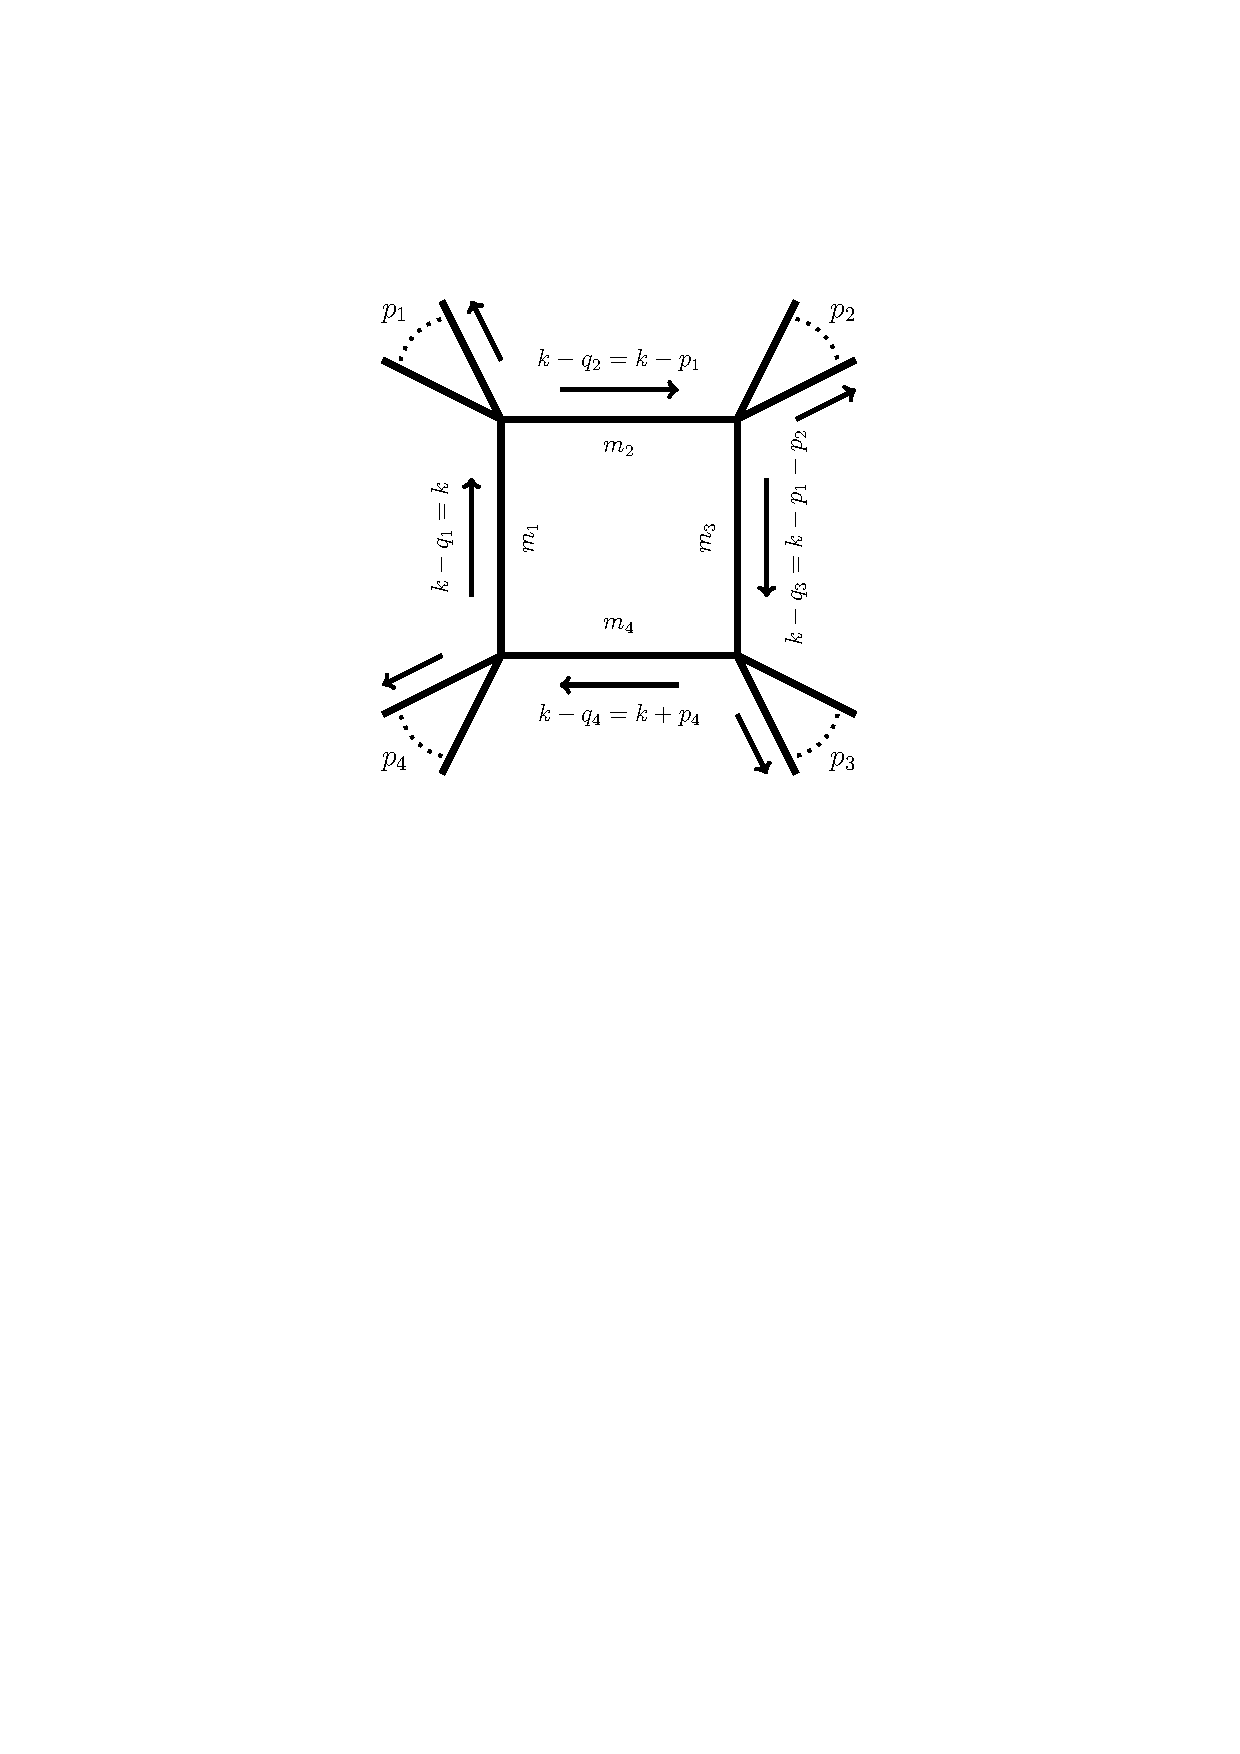
\includegraphics[width=0.5\textwidth]{ch3_loopamps/figures/box-gen.pdf}
  \caption{A general box configuration labelled according to the conventions of section~\ref{sssec:4dbox}. The arrows denote the direction of the momenta.}
  \label{fig:generalbox}
\end{figure}

Our aim is to define an irreducible numerator, $\Delta_{1|2|3|4}$, that
parametrises all possible loop-momentum dependence in the numerator of the box
topology. In other words, we are interested in taking the quadruple cut of the
numerator function. Working at the integrand level, we re-use the notation
$\mathcal{C}_{1|2|3|4}$ used for the amplitudes in section~\ref{sec:3.3} to
indicate the inverse propagators are being set to zero:
$\mathcal{C}_{1|2|3|4}(f) \coloneqq f |_{D_i\to 0}$ for all $i=1,\ldots,4$. As
we have just ascertained that the loop-momentum dependence of $\vec{\alpha}$ is
entirely in terms of inverse propagators, the relevant part of the
loop-momentum parametrisation in \eqn{eq:momparam} depends on only one
loop-momentum dependent scalar product, $k\cdot\omega$, which we refer to as
the \emph{irreducible scalar product} (ISP). All terms in $\vec{\alpha}$
proportional to inverse propagators fall into sub-topologies which will be
dealt with later. For a renormalisable gauge theory\footnote{For other
theories, effective theories or gravity the only change would be to increase
the upper limit on the sum.} the dependence of the numerator must then have the
form
\begin{equation}
  \Delta_{1|2|3|4}(k\cdot\omega) = \sum_{i=0}^4 c_{i;1|2|3|4} \, (k\cdot\omega)^i \,.
  \label{eq:box4dintegrandparam}
\end{equation}
There is however one more constraint on the loop-momentum dependence of the numerator that comes from the
condition $D_1= 0$:
\begin{equation}
  \mathcal{C}_{1|2|3|4} \left( k^2 -m_1^2 \right) = \mathcal{C}_{1|2|3|4} \left( k_{\parallel}^2  \right) + (k\cdot\omega)^2 \, \omega^2 - m_1^2  = 0 \,.
  \label{eq:boxksqcondition}
\end{equation}
Since $\mathcal{C}_{1|2|3|4} \bigl( k_{\parallel}^2 \bigr)$ is a function of the external invariants
only---the inverse propagators are set to zero---it is a constant as far as the loop-momentum dependence goes. 
The condition~\eqref{eq:boxksqcondition} therefore states that monomials with more than one power of $k\cdot\omega$ are \textit{reducible}.
We may thus write the numerator of this box configuration as
\begin{equation}
  \Delta_{1|2|3|4}(k\cdot\omega) = c_{0;1|2|3|4} + c_{1;1|2|3|4} \, (k\cdot\omega) \,,
  \label{eq:box4dintegrandparam}
\end{equation}
where the rational coefficients $c_0$ and $c_1$ can be determined for an
arbitrary process from the cuts of Feynman diagrams or, as we have described
earlier in this chapter, from the product of tree-level amplitudes. To put
this more concretely, we can use the explicit loop-momentum solutions to \eqn{eq:boxksqcondition},
\begin{equation}
  k^{\pm,\mu} = \mathcal{C}_{1|2|3|4}\left(k_{\parallel}^\mu\right) \pm \sqrt{\frac{m_1^2-\mathcal{C}_{1|2|3|4}\bigl(k_{\parallel}^2\bigr)}{\omega^2}} \, \omega^\mu \,,
\end{equation}
to write down an expression for the quadruple cut of an arbitrary one-loop amplitude:
\begin{align}
  \mathcal{C}_{1|2|3|4} \left(A_n^{(1),[4-2\eps]}\right) 
  & = \int_k \Delta_{1|2|3|4} (k \cdot \omega) \, \left(\prod_{i=1}^4 (-2\pi\i) \, \delta^{(+)}(D_i) \right)   \nonumber\\
  & = \int_k \biggl(I^{(1)} \prod_{i=1}^4 D_i \biggr) \,\left(\prod_{i=1}^4 (-2\pi\i) \, \delta^{(+)}(D_i) \right) \,,
  \label{eq:quadcutrelation1}
\end{align}
where $I^{(1)}$ represents the integrand of the one-loop amplitude as
introduced previously. Identifying the integrands subject to the delta function
constraints leads us to the algebraic relation
\begin{align}
  \Delta_{1|2|3|4} (k \cdot \omega) \bigg|_{D_i = 0} = \biggl(I^{(1)} \prod_{i=1}^4 D_i \biggr) \bigg|_{D_i = 0}.
  \label{eq:quadcutrelation2}
\end{align}
If we had explicitly performed the integration over the delta functions in
\eqn{eq:quadcutrelation1} we would also obtain a Jacobian factor but it would
cancel on both sides of the relation.  The integrand $I^{(1)}$ could be
obtained by simply taking the subset of Feynman diagrams which have the same
four propagators and substituting the on-shell values of the loop momenta
$k^\pm$. In a physical gauge,\footnote{In exercise~\ref{Ex:1.7} we showed in
the light-like axial gauge that the numerator of the propagator can be written
as the product of polarisation vectors in the on-shell limit times a factor of
$\i$. Incidentally, this is the origin of the factors of $\i$ which accompany
the tree-level amplitudes in the factorisation on the cuts, see e.g.\
\eqn{eq:quadcuteq}.} it is easy to see that this subset
of diagrams may also be written as the product of tree-level amplitudes summed
over the internal helicity configurations:
\begin{align}
  \Biggr( I^{(1)} \prod_{i=1}^4 D_i \Biggl) \Biggl|_{k^\pm} & = \nonumber\\
  %
  & \hspace{-2.15cm}  \sum_{h_i=\pm} \Bigg[ \i \, A^{(0)}\Bigl((-k^\pm)^{-h_1},p_1,(k^\pm-p_1)^{h_2} \Bigr) \,
  \i \, A^{(0)}\Bigl((-k^\pm+p_1)^{-h_2},p_2,(k^\pm-p_{12})^{h_3}\Bigr) \, \nonumber\\
  & \hspace{-2.15cm} \phantom{ \sum_{h_i=\pm} \Bigg[} \, \i \, A^{(0)}\Bigl((-k^\pm+p_{12})^{-h_3},p_3,(k^\pm+p_4)^{h_4}\Bigr) \,
  \i \, A^{(0)}\Bigl((-k^\pm-p_4)^{-h_4},p_4,(k^\pm)^{h_1}\Bigr) \Bigg] \nonumber\\
  & = \Delta_{1|2|3|4}(k^\pm\cdot\omega) \,.
  \label{eq:quadcuteq}
\end{align}
%
Using the on-shell values for the ISP,
\begin{equation}
  k^\pm\cdot \omega = \pm \sqrt{\frac{m_1^2-\mathcal{C}_{1|2|3|4}\bigl(k_{\parallel}^2\bigr)}{\omega^2}} \,,
  \label{eq:onshellISPsol}
\end{equation}
we can invert \eqn{eq:quadcuteq} to find solutions for the rational coefficients $c_{i;1|2|3|4}$ of the
parametrisation of $\Delta_{1|2|3|4}$ in \eqn{eq:box4dintegrandparam}. We obtain
\begin{align}
  c_{0;1|2|3|4} &= \frac{1}{2}\left( \overline{I}^{(1)}(k^+) +  \overline{I}^{(1)}(k^-) \right), \\
  c_{1;1|2|3|4} &= \frac{1}{2}\sqrt{\frac{\omega^2}{m_1^2-\mathcal{C}_{1|2|3|4}\bigl( k_{\parallel}^2 \bigr)}} \left( \overline{I}^{(1)}(k^+) -  \overline{I}^{(1)}(k^-) \right) \,,
\end{align}
where we introduced the short-hand notation
\begin{align}
\overline{I}^{(1)}(k^\pm) \coloneqq \Biggr( I^{(1)} \prod_{i=1}^4 D_i \Biggl) \Biggl|_{k^\pm} \,.
\end{align}
This proves the averaging prescription that we already applied during generalised unitarity cut computations in section~\ref{sec:3.3}. 
Having determined both coefficients from the on-shell cut, we see that the contribution to the amplitude is simply
\begin{equation}
  \int_k \frac{\Delta_{1|2|3|4}(k)}{(-D_1) (-D_2) (-D_3) (-D_4)}  = c_{0;1|2|3|4} \, F^{[4-2\eps]}_4(p_1,p_2,p_3)[1] \,,
  \label{eq:Delta4integrated}
\end{equation}
as the second, spurious, element integrates to zero following the arguments
presented earlier in section~\ref{ssec:transverse} regarding transverse integration. Notice that the minus signs on the inverse propagators have been put in to match the conventions for the Feynamn integrals in \eqn{eq:oneloopintegraldef}.

We have now demonstrated two important facts: a general basis for the
(four-dimensional) box part of any one-loop amplitude is simply the scalar box
integral, and its coefficient may be extracted by a purely algebraic
procedure using generalised unitarity cuts.

\subsubsection{The triangle integrand in four dimensions}

The procedure for determining the remaining parts of the amplitude and
establishing a complete integral basis is to reduce the number of cut
propagators to the triangle (then bubble, then tadpole) contributions.

We begin in exactly the same fashion as the box configuration by defining the inverse propagators according to
\begin{align}  \label{eq:triprops}
D_1 = k^2-m_1^2 \,, \qquad
D_2 = (k-p_1)^2 - m_2^2 \,, \qquad
D_3 = (k-p_{12})^2 - m_3^2 \,,
\end{align}
and parametrise the loop momenta using two orthogonal spurious vectors $\omega_i$,
\begin{align} 
\begin{aligned}
  k^\mu &= k_{\parallel}^\mu + (k\cdot\omega_1) \, \omega_1^{\mu} + (k\cdot\omega_2) \, \omega_2^{\mu} \,, \\
  k_{\parallel}^\mu &= \vec{\alpha}\cdot \vec{v}^\mu \,,
\end{aligned}
  \label{eq:momparamtri}
\end{align}
where $\vec{v}^{\mu} = \{p_1^{\mu},p_2^{\mu}\}$ with $\omega_i^{\mu} p_{j\, \mu} = 0$ for $i,j=1,2$, and $\vec{\alpha} =
\{\alpha_1, \alpha_2\}$. We have seen the explicit construction of the physical
and spurious spaces in section~\ref{ssec:transverse} so it is clear that
$\vec{\alpha}$ only depends on the inverse propagators, and hence on the triple cut
have no loop-momentum dependence. We therefore have two ISPs with which to
parametrise our triangle integrand: $k\cdot\omega_1$ and $k\cdot\omega_2$. For a
renormalisable gauge theory the maximum tensor rank is three and so a general
parametrisation is
\begin{equation}
  \Delta_{1|2|3}(k\cdot\omega_1, k\cdot\omega_2) = \sum_{i,j} c_{ij}  \,(k\cdot\omega_1)^i \, (k\cdot\omega_2)^j \,,
  \label{eq:triparam1}
\end{equation}
with $i+j \leq3$. This parametrisation is subject to the constraint
\begin{equation}
  \mathcal{C}_{1|2|3} \left( k^2 - m_1^2 \right) = \mathcal{C}_{1|2|3} \left( k_{\parallel}^2 \right) - m_1^2 + (k\cdot\omega_1)^2 \omega_1^2 + (k\cdot\omega_2)^2 \omega_2^2 = 0 \,.
  \label{eq:triksqcondition}
\end{equation}
It is slightly more difficult to apply this constraint to find a general
parametrisation since we now have multivariate polynomials. One could attempt
to deploy the mathematical technology to deal with such problems, introducing a
polynomial ordering and performing polynomial division with respect to a
Gr\"{o}bner basis,\footnote{Many computer algebra systems now come equipped with
decent implementations of polynomial division algorithms, so this can be a
practical method.} but it is easier to analyse this case by hand and
we will find an extremely convenient choice. Firstly we expand
\eqn{eq:triparam1} explicitly,
\begin{align}
  \Delta_{1|2|3}&(k\cdot\omega_1, k\cdot\omega_2) = c_{00}
  + c_{10} (k\cdot\omega_1) 
  + c_{01} (k\cdot\omega_2) \nonumber\\& 
  + c_{20} (k\cdot\omega_1)^2
  + c_{11} (k\cdot\omega_1) (k\cdot\omega_2) 
  + c_{02} (k\cdot\omega_2)^2 \nonumber\\& 
  + c_{30} (k\cdot\omega_1)^3
  + c_{21} (k\cdot\omega_1)^2 (k\cdot\omega_2)
  + c_{12} (k\cdot\omega_1) (k\cdot\omega_2)^2
  + c_{03} (k\cdot\omega_2)^3 \,.
  \label{eq:triparam2}
\end{align}
Removing all monomials with even powers of $k\cdot\omega_2$ would be a valid choice
and eliminate the implicit dependence on three of the monomials. The resulting
integrand parametrisation would still contain an integral quadratic in
$k\cdot\omega_1$, which we have seen does not vanish after integration. In the example of transverse integration from \eqn{eq:triwsqtransverseint} we saw that the integral of
$(k\cdot\omega_1)^2$ is the same as $(k\cdot\omega_2)^2$ up to a normalisation.
Therefore, in order to obtain a simple result after (transverse) integration, we choose
\begin{align} 
\begin{aligned}
  \Delta_{1|2|3}&(k\cdot\omega_1, k\cdot\omega_2) = c_{0;1|2|3}
  + c_{1;1|2|3} (k\cdot\omega_1) 
  + c_{2;1|2|3} (k\cdot\omega_2) \\& 
  + c_{3;1|2|3} \left((k\cdot\omega_1)^2 - \frac{\omega_1^2}{\omega_2^2} (k\cdot\omega_2)^2 \right)
  + c_{4;1|2|3} (k\cdot\omega_1) (k\cdot\omega_2) \\&
  + c_{5;1|2|3} (k\cdot\omega_1)^3
  + c_{6;1|2|3} (k\cdot\omega_1)^2 (k\cdot\omega_2) \,,
\end{aligned}
\label{eq:triparam}
\end{align}
where we constructed a spurious integral from the linear combination of $(k\cdot\omega_1)^2$ and $(k\cdot\omega_2)^2$.
As a result, after integration, all terms except the scalar integral coefficient vanish:
\begin{equation}
  \int_k \frac{\Delta_{1|2|3}(k\cdot\omega_1, k\cdot\omega_2)}{(-D_1) (-D_2) (-D_3)}  = c_{0;1|2|3} \, F^{[4-2\eps]}_3(p_1,p_2)[1] \,.
  \label{eq:Delta3integrated}
\end{equation}
The extraction of the rational coefficients can be performed algebraically by
using the information computed using the quadruple cuts as input. Following the
box example as a reference we write
\begin{align}
  \mathcal{C}_{1|2|3} & \left( A^{(1),[4-2\eps]}_n \right) \nonumber\\&
  = \int_k \left( -\Delta_{1|2|3}(k\cdot\omega_1, k\cdot\omega_2)  + \sum_X \frac{\Delta_{1|2|3|X}(k\cdot\omega)}{D_X} \right) \left(\prod_{i=1}^3 (-2\pi\i)\, \delta^{(+)}(D_i)\right) \nonumber\\&
  = \int_k I^{(1)}(k) \left(\prod_{i=1}^3 D_i \, (-2\pi\i)\, \delta^{(+)}(D_i) \right) \,,
\end{align}
which implies that
\begin{align}
  -\Delta_{1|2|3}(k\cdot\omega_1, k\cdot\omega_2) \bigg|_{D_i = 0} = \left( I^{(1)}(k) \prod_{i=1}^3 D_i - \sum_X \frac{\Delta_{1|2|3|X}(k\cdot\omega)}{D_X} \right) \bigg|_{D_i = 0} \,.
  \label{eq:triplecuteq}
\end{align}
The sum over $X$ for the box numerators indicates that we must include all
boxes that share the three propagators $\{D_1,D_2,D_3\}$, with $D_X$ being the
fourth propagator which completes the box.  Denoting the box configurations in
the subtraction as $1|2|3|X$ is a slight abuse of notation, and we give an
explicit example below to clarify.

The integrand factorises into tree amplitudes as before,
\begin{align} \begin{aligned}
  \left( I^{(1)}(k) \prod_{i=1}^3 D_i \right) \bigg|_{D_i = 0} = \sum_{h_i=\pm} \bigg[ &
   \i \, A^{(0)}\Bigl((-k)^{-h_1},p_1,(k-p_1)^{h_2} \Bigr) \\
   &  \i \, A^{(0)}\Bigl((-k+p_1)^{-h_2},p_2,(k-p_{12})^{h_3}\Bigr) \\
   &  \i \, A^{(0)}\Bigl((-k+p_{12})^{-h_3},p_3,(k)^{h_1}\Bigr) \bigg] \bigg|_{D_i = 0} \,,
\end{aligned} \end{align}
but on this occasion solving the on-shell constraints will lead to a family of
loop momenta parametrised by a single variable. The choice of this
parametrisation is not an immediate issue since it is more important to realise
that the triple cut condition in \eqn{eq:triplecuteq} must be valid
for any value of the free variable, which is sufficient to find the conditions
necessary to fix the rational coefficients $c_{i;1|2|3}$.

\begin{example}{Example: Subtraction terms for a six-point amplitude}
  Since the sum over $X$ and the cut notation $1|2|3|X$ in \eqn{eq:triplecuteq}
  are schematic, it is helpful to see an explicit example. Consider the
  application to an amplitude with six external legs where we are computing the
  triple cut $12|34|56$. The sum over $X$ for the box subtraction terms would
  then indicate the following set:
  \begin{equation}
    \bigl\{ 1|2|34|56 \,, 12|3|4|56 \,, 12|34|5|6 \bigr\}\,.
  \end{equation}
\end{example}

\subsubsection{The bubble integrand in four dimensions}

At this point the integrand reduction strategy of Ossola, Papadopoulos and
Pittau should be clear: continue to reduce the on-shell constraints on the
propagators until all the integral basis coefficients have been determined.

The equation for the irreducible numerator in the case of bubble
configurations, $\Delta_{1|2}$, is constructed from three irreducible scalar
products: $k\cdot\omega_1$, $k\cdot\omega_2$ and $k\cdot\omega_3$. Note that
$\omega_1$ and $\omega_2$ are not the same spurious vectors for the triangle
configuration. We will consider a configuration with inverse propagators
\begin{align}
  D_1 = k^2-m_1^2 \,, \qquad \qquad D_2 = (k-p_1)^2 - m_2^2 \,,
  \label{eq:bubbleprops}
\end{align}
and parametrise the loop momenta using the three orthogonal spurious vectors $\omega_i$ as
\begin{align}   \label{eq:momparambubble}
  k^\mu & = k^{\mu}_{\parallel} + (k\cdot\omega_1) \, \omega_1^\mu + (k\cdot\omega_2) \, \omega_2^\mu + (k\cdot\omega_3) \, \omega_3^\mu \,, \\
  k^{\mu}_{\parallel} & = \vec{\alpha} \cdot \vec{v}^\mu \,,
\end{align}
where $\vec{v}^\mu = \{p_1^\mu\}$ and $\vec{\alpha}=\{\alpha_1\}$. The remainder of the derivation we leave as an exercise, although perhaps the result is already clear by analogy to the triple cut case.

\begin{exer}{Parametrising the bubble integrand}
\label{Ex:3.6}
\vspace{-0.6cm}
\begin{enumerate}[a)]
\item Show that the irreducible numerator of a general bubble configuration can be written as
\begin{align} \label{eq:bubble_num_param}
\begin{aligned}
  \Delta_{1|2}&(k\cdot\omega_1, k\cdot\omega_2, k\cdot\omega_3) = c_{0;1|2} \\
 & + c_{1;1|2} (k\cdot\omega_1) 
  + c_{2;1|2} (k\cdot\omega_2) 
  + c_{3;1|2} (k\cdot\omega_3) \\ 
&  + c_{4;1|2} (k\cdot\omega_1) (k\cdot\omega_2) 
  + c_{5;1|2} (k\cdot\omega_1) (k\cdot\omega_3) 
  + c_{6;1|2} (k\cdot\omega_2) (k\cdot\omega_3) \\  
 & + c_{7;1|2} \left((k\cdot\omega_1)^2 - \frac{\omega_1^2}{\omega_3^2} (k\cdot\omega_3)^2 \right)
  + c_{8;1|2} \left((k\cdot\omega_2)^2 - \frac{\omega_2^2}{\omega_3^2} (k\cdot\omega_3)^2 \right) \,,
\end{aligned}
\end{align}
which results in
\begin{align}
  \int_k \frac{\Delta_{1|2}(k\cdot\omega_1, k\cdot\omega_2, k\cdot\omega_3)}{(-D_1) (-D_2)}  = c_{0;1|2} \, F^{[4-2\eps]}_2(p_1)[1] \,.
\end{align}
\item Show that the irreducible numerator can be determined on the double cut from
\begin{align}
\begin{aligned}
  \Delta_{1|2}&(k\cdot\omega_1, k\cdot\omega_2, k\cdot\omega_3) \bigg|_{D_i = 0} =
     \bigg( I^{(1)}(k) \prod_{i=1}^2 D_i \\&
     + \sum_X \frac{\Delta_{1|2|X}(k\cdot\omega_1^{X}, k\cdot\omega_2^{X})}{D_X} - \sum_{Y,Z} \frac{\Delta_{1|2|Y|Z}(k\cdot\omega^{YZ})}{D_Y D_Z} \bigg) \bigg|_{D_i = 0} \,,
\end{aligned}
  \label{eq:doublecuteq}
\end{align}
where the sum on $X$ indicates all triangle configurations, and the sum on $Y,Z$ indicates all box configurations. Again the sign on the triangle irreducible numerator $\Delta_{1|2|X}$ matches our sign conventions on the Feynman integrals.
\end{enumerate}
For the solution see \hyperref[Sol:3.6]{chapter~5}.
\end{exer}

For massless theories such as Yang-Mills theory we have now completed an
algebraic approach for the determination of the four-dimensional, or cut
constructible, part of the one-loop integrand. In massive theories there are
still contributions for integrals which only depend on the mass: tadpoles and
bubbles on external massive legs. One can continue to apply the integrand
reduction procedure to these cases and a full analysis can, for example, be
found in reference~\cite{ch3_Ellis:2011cr}. There is a subtlety in the method
though since the unrenormalised amplitude diverges when applying bubble cuts on
external lines and so we cannot factorise into the product of tree amplitudes
without additional regulators. The issue is connected with wave-function
renormalisation and the interested reader can find further information in the
literature~\cite{ch3_Ellis:2008ir,ch3_Britto:2011cr,ch3_Badger:2017gta}.

\subsection{$D$-dimensional integrands and rational terms}

The results of section~\ref{ssec:4dintegrandbasis} gave us confidence in the
proposed general one-loop formula in \eqn{eq:oneloop4dbasis}. The fact
that we found only scalar integrals after removing the spurious terms was
consistent with the tensor integral reduction method introduced in section~\ref{sec:3.4}, so we can consider this result as a confirmation of the latter. The
integrand-level matching of cut diagrams to irreducible numerators enabled the
\textit{algebraic} determination of the integral coefficients, leaving the
remaining integration of the basis integrals as a separate problem. That
problem is not to be underestimated of course and is the subject of the next
chapter.

The aim for the rest of this section is to extend our analysis to $D=4-2\eps$
dimensional integrands and amplitudes. This means that we can no longer avoid
the contribution of the pentagon which now becomes the starting point for the
top down integrand reduction approach of Ossola, Papdopoulos and Pittau. 

\subsubsection{The pentagon integrand}

Since there are four independent external momenta in the pentagon configuration
there is no spurious space. In exercise~\ref{Ex:3.5} we showed that the pentagon
configuration was completely reducible in four dimensions. In $D=4-2\eps$, we
need to clarify this point and to extend our four dimensional analysis of the
integrand. The decomposition of the transverse space gives us the starting
point. For concreteness we can specify the propagators,
\begin{align}
\begin{alignedat}{3}
& D_1 = k^2-m_1^2\,, && D_2 = (k-p_1)^2 - m_2^2\,, \qquad && D_3 = (k-p_{12})^2 - m_3^2 \,, \\
& D_4 = (k-p_{123})^2 - m_4^2\,, \qquad && D_5 = (k+p_5)^2 - m_5^2\,, && \\
\end{alignedat}
\label{eq:boxprops}
\end{align}
the spanning set of external momenta (which are four dimensional),
\begin{align}
\vec{v}^{\mu} = \{ p_1^{\mu}, p_2^{\mu}, p_3^{\mu}, p_4^{\mu} \} \,,
\end{align}
and the parametrisation of the loop momentum,
\begin{equation}
  k^\mu = \vec{\alpha}\cdot \vec{v}^\mu + k^{\mu, [-2\eps]} \,.
\end{equation}
Note that in this case there is no spurious space, as the external momenta $\vec{v}^{\mu}$ are sufficient to span the entire four-dimensional space.
As before, the coefficients $\vec{\alpha}$ of the spanning vectors of the physical
space are functions of the propagators and the external invariants. The
on-shell condition $D_1=0$ gives the key constraint for the determination of
the integrand basis,
\begin{equation}
  k^2 - m_1^2 = \vec{\alpha}\cdot G \cdot \vec{\alpha}^{\top} - \mu_{11} -m_1^2 = 0 \,,
  \label{eq:pentmucondition}
\end{equation}
where we have explicitly used the Gram matrix $G_{ij} = \vec{v}_i^{\mu}
\vec{v}_{j\,\mu}$. After applying the four on-shell conditions
$\{D_2,D_3,D_4,D_5\}=0$, the only ISP in this equation is $\mu_{11}$, and we
see that on the quintuple cut this ISP will be a constant expression written in
terms of external invariants. We may therefore parametrise the irreducible
numerator as
\begin{equation}
  \Delta_{1|2|3|4|5}(\mu_{11}) = \sum_{i=0}^2 c_{i;1|2|3|4|5} \, \mu_{11}^i \,,
\end{equation}
subject to the constraint in \eqn{eq:pentmucondition}. A minimal solution
to this would seem to take just the scalar pentagon as a basis integrand,
however this would not be consistent with the complete reduction of the
pentagon in four dimensions. The next-to-minimal choice is a single power of $\mu_{11}$,
\begin{equation}
  \Delta_{1|2|3|4|5}(\mu_{11}) = c_{1;1|2|3|4|5} \, \mu_{11} \,,
\end{equation}
which vanishes explicitly in the $D\to 4$ limit as we had previously argued. We
will not explicitly perform the integration but simply state that it is
possible to show the integral vanishes up to $\mathcal{O}(\eps)$: 
\begin{equation}
  \int_k \frac{\Delta_{1|2|3|4|5}(\mu_{11})}{D_1 D_2 D_3 D_4 D_5}  = \mathcal{O}(\eps) \,. 
\end{equation}

\subsubsection{Extending the box, triangle and bubble integrand basis to $D=4-2\eps$ dimensions}

The integrand reduction procedure is now rather easy to extend into
$D$-dimensions, since all we have to do is track the additional dependence on
the extra-dimensional ISP~$\mu_{11}$. The box irreducible numerator then becomes a polynomial in two ISPs,
\begin{equation}
  \Delta_{1|2|3|4}(k\cdot\omega, \mu_{11}) = \sum_{i,j} c_i \, (k\cdot\omega)^i \mu_{11}^j \,,
\end{equation}
where $i+2j<4$, and
\begin{equation}
  \mathcal{C}_{1|2|3|4} \left( k^2 - m_1^2 \right) = \mathcal{C}_{1|2|3|4} \left( k_{\parallel}^2  \right) - m_1^2 + (k\cdot\omega)^2 \omega^2 - \mu_{11} = 0\,.
  \label{eq:boxksqconditionD}
\end{equation}
The simplest solution is to eliminate $\mu_{11}$ from the parametrisation
completely, leaving five monomials in the ISP $k\cdot\omega$. Two of these
monomials would not vanish after integration however and again, as in the
pentagon case, the $D\to 4$ limit would not match our four-dimensional
analysis. Instead we choose the two terms from the four-dimensional
parametrisation and three more monomials proportional to $\mu_{11}$, 
\begin{align}
  \Delta_{1|2|3|4}(k\cdot\omega, \mu_{11}) & =  c_{0;1|2|3|4}
  + c_{1;1|2|3|4} \, (k\cdot\omega)
  + c_{2;1|2|3|4} \, \mu_{11} \nonumber\\
  & \phantom{= {}} + c_{3;1|2|3|4} \, (k\cdot\omega) \, \mu_{11}
  + c_{4;1|2|3|4} \, \mu_{11}^2 \,.
  \label{eq:boxparamD}
\end{align}
The result integrating this expression turns out to be incredibly simple but,
as before with the pentagon, requires some additional integration technology.
In $4-2\eps$ dimensions it turns out that the integral with $\mu_{11}$ in the
denominator vanishes up to $\mathcal{O}(\eps)$ while the $\mu_{11}^2$ integral
gives rise to a finite, and rational, contribution,
\begin{align}
  \int_k &\frac{\Delta_{1|2|3|4}(k\cdot\omega, \mu_{11})}{(-D_1) (-D_2) (-D_3) (-D_4)} \nonumber \\
  & = c_{0;1|2|3|4} \, F^{[4-2\eps]}_4(p_1,p_2,p_3)[1]
    + c_{2;1|2|3|4} \, F^{[4-2\eps]}_4(p_1,p_2,p_3)[\mu_{11}] \nonumber\\
  & \phantom{= {}} + c_{4;1|2|3|4} \, F^{[4-2\eps]}_4(p_1,p_2,p_3)[\mu_{11}^2] \nonumber\\&
    = 
    c_{0;1|2|3|4} \, F^{[4-2\eps]}_4(p_1,p_2,p_3)[1] - \frac{1}{6} c_{4;1|2|3|4} + \mathcal{O}(\eps) \,.
\end{align}
The final steps are to repeat the analysis for the triangle and bubble, and so we can quote the results for the triangle irreducible numerator,
\begin{align}
  \Delta_{1|2|3}&(k\cdot\omega_1, k\cdot\omega_2, \mu_{11}) = c_{0;1|2|3}
  + c_{1;1|2|3} \, (k\cdot\omega_1) 
  + c_{2;1|2|3} \, (k\cdot\omega_2) \nonumber\\& 
  + c_{3;1|2|3} \, \left((k\cdot\omega_1)^2 - \frac{\omega_1^2}{\omega_2^2} (k\cdot\omega_2)^2 \right)
  + c_{4;1|2|3} \, (k\cdot\omega_1) (k\cdot\omega_2) \nonumber\\& 
  + c_{5;1|2|3} \, (k\cdot\omega_1)^3
  + c_{6;1|2|3} \, (k\cdot\omega_1)^2 (k\cdot\omega_2)\nonumber\\&
  + c_{7;1|2|3} \, \mu_{11} 
  + c_{8;1|2|3} \, (k\cdot\omega_1) \, \mu_{11} 
  + c_{9;1|2|3} \, (k\cdot\omega_2) \, \mu_{11} \,,
  \label{eq:triparamD}
\end{align}
and its integrated form,
\begin{align}
  \int_k &\frac{\Delta_{1|2|3}(k\cdot\omega_1, k\cdot\omega_2, \mu_{11})}{(-D_1) (-D_2) (-D_3)} \nonumber\\& =
      c_{0;1|2|3} \, F^{[4-2\eps]}_3(p_1,p_2)[1]
    + c_{7;1|2|3} \, F^{[4-2\eps]}_3(p_1,p_2)[\mu_{11}] \nonumber\\&
    = 
    c_{0;1|2|3} \, F^{[4-2\eps]}_3(p_1,p_2)[1] - \frac{1}{2} c_{7;1|2|3} + \mathcal{O}(\eps) \,,
\end{align}
and also the bubble irreducible numerator
\begin{align}
  \Delta_{1|2}&(k\cdot\omega_1, k\cdot\omega_2, k\cdot\omega_3, \mu_{11}) = c_{0;1|2}
  + c_{1;1|2} \, (k\cdot\omega_1) 
  + c_{2;1|2} \, (k\cdot\omega_2) \nonumber\\& 
  + c_{3;1|2} \, (k\cdot\omega_3) 
  + c_{4;1|2} \, \left((k\cdot\omega_1)^2 - \frac{\omega_1^2}{\omega_3^2} (k\cdot\omega_3)^2 \right)
  + c_{5;1|2} \, \left((k\cdot\omega_2)^2 - \frac{\omega_2^2}{\omega_3^2} (k\cdot\omega_3)^2 \right) \nonumber\\&
  + c_{6;1|2} \, (k\cdot\omega_1) (k\cdot\omega_2) 
  + c_{7;1|2} \, (k\cdot\omega_1) (k\cdot\omega_3) 
  + c_{8;1|2} \, (k\cdot\omega_2) (k\cdot\omega_3) 
  + c_{9;1|2} \, \mu_{11} \,,
  \label{eq:bubparamD}
\end{align}
and its integrated form,
\begin{align}
  \int_k &\frac{\Delta_{1|2}(k\cdot\omega_1, k\cdot\omega_2, k\cdot\omega_3, \mu_{11})}{(-D_1) (-D_2)} \nonumber\\
  & \quad =
      c_{0;1|2} \, F^{[4-2\eps]}_2(p_1)[1]
    + c_{9;1|2} \, F^{[4-2\eps]}_2(p_1)[\mu_{11}] \nonumber\\
    & \quad = 
    c_{0;1|2} \, F^{[4-2\eps]}_2(p_1)[1] - \frac{p_1^2-m_1^2-m_2^2}{6} \, c_{9;1|2} + \mathcal{O}(\eps) \,.
\end{align}
When integrating the irreducible numerators we have used the following results for integrals in $D=4-2\eps$ dimensions:
\begin{align}
  F^{[4-2\eps]}_5(p_1,p_2,p_3,p_4)[\mu_{11}] &= \mathcal{O}(\eps) \,, \\
  F^{[4-2\eps]}_4(p_1,p_2,p_3)[\mu_{11}] &= \mathcal{O}(\eps) \,, \\
  F^{[4-2\eps]}_4(p_1,p_2,p_3)[\mu_{11}^2] &= -\frac{1}{6} + \mathcal{O}(\eps) \,, \\
  F^{[4-2\eps]}_3(p_1,p_2)[\mu_{11}] &= -\frac{1}{2} + \mathcal{O}(\eps) \,, \\
  F^{[4-2\eps]}_2(p_1)[\mu_{11}] &= -\frac{p_1^2-m_1^2-m_2^2}{6} + \mathcal{O}(\eps) \,.
\end{align}
Explicitly proving these results requires technology for loop integration that
we have not yet introduced. One interesting observation~\cite{ch3_Bern:1995db} is that the
$\mu_{11}$ numerators give rise to dimension-shifted integrals:
\begin{equation}
  F^{[4-2\eps]}_n(p_1,\ldots,p_{n-1})[\mu_{11}^r] = \left(\prod_{s=0}^{r-1}(s-\eps) \right) \, F^{[4+2r-2\eps]}_n(p_1,\ldots,p_{n-1})[1] \,.
  \label{eq:dimshift}
\end{equation}
The fact that the relation is proportional to $\eps$ shows that we are only
interested in the poles of the dimension-shifted integrals. Shifting the
dimension up improves the infrared behaviour and so all the possible poles in
the dimension-shifted integrals are of UV origin. The vanishing of the pentagon
and box integrals with the $\mu_{11}$ numerator can then be understood since the
integrand-level power-counting argument shows that the $(6-2\eps)$-dimensional scalar
integrals are UV finite.


\begin{exer}{Dimension-shifting relation at one loop}
\label{Ex:3.DimShift}
%
Prove the dimension-shifting relation~\eqref{eq:dimshift}~\cite{ch3_Bern:1995db}. Assume that the external momenta $p_i$ are four dimensional, and decompose the loop momentum into a four- and an extra-dimensional parts (see section~\ref{ssec:transverse}). The key of the proof is that the integrand of the integral on the LHS of \eqn{eq:dimshift} depends on the loop momentum only through its four-dimensional part and $\mu_{11}$.
Switch to radial and angular coordinates in the extra-dimensional subspace, carry out the angular integration, and absorb the factor of $\mu_{11}^r$ in the numerator into the radial part of a $(2r-2\eps)$-dimensional loop-integration measure. Use the following Gamma-function identity to simplify the ratio of the angular integrals,
\begin{align} \label{eq:gamma_ratio}
\frac{\Gamma(r-\eps)}{\Gamma(-\eps)} = \prod_{s=0}^{r-1} (s-\eps) \,.
\end{align}
We will prove the above in the solution of exercise~\ref{Ex:ExpGamma}. 
Finally, putting together the $(2r-2\eps)$-dimensional and the four-dimensional loop-integration measures gives the RHS of \eqn{eq:dimshift}.
For the solution see \hyperref[Sol:3.DimShift]{chapter~5}.

\end{exer}



\subsection{Final expressions for one-loop amplitudes in $D$-dimensions}

We have now completed the analysis at one loop. We have used a general integrand
parametrisation to prove the basis used in \eqn{eq:oneloop4dbasis} but
have now identified the connection between the rational terms and the
extra-dimensional terms missed by the $4D$ cuts. We can therefore give an
explicit formula for the rational term $R$:
\begin{align}
  A^{(1),[4-2\eps]}_n&(1,\ldots,n) = \nonumber\\&
    \sum_{1\leq i_1<i_2<i_3<i_4\leq n} \i \, c_{0;i_1|i_2|i_3|i_4} \, F^{[4-2\eps]}_4(p_{i_1,i_2-1},p_{i_2,i_3-1},p_{i_3,i_4-1})[1]\nonumber\\&
  + \sum_{1\leq i_1<i_2<i_3\leq n} \i \, c_{0;i_1|i_2|i_3} \, F^{[4-2\eps]}_3(p_{i_1,i_2-1},p_{i_3,i_3-1})[1]\nonumber\\&
  + \sum_{1\leq i_1<i_2\leq n} \i \, c_{0;i_1|i_2} \, F^{[4-2\eps]}_2(p_{i_1,i_2-1})[1]\nonumber\\&
  + \sum_{1\leq i_1\leq n} \i \, c_{0;i_1} \, F^{[4-2\eps]}_1(p_{i_1})[1]\nonumber\\&
  + R(1,\ldots,n) + \mathcal{O}(\eps) \,,\\
  R(1,\ldots,&n) = 
  -\frac{1}{6} \sum_{1\leq i_1<i_2<i_3<i_4\leq n} \i \, c_{4;i_1|i_2|i_3|i_4} \nonumber\\&
  -\frac{1}{2} \sum_{1\leq i_1<i_2<i_3\leq n} \i \, c_{7;i_1|i_2|i_3} \nonumber\\&
  -\frac{1}{6} \sum_{1\leq i_1<i_2\leq n}  \left(p_{i_1,i_2-1}^2 - m_{i_1}^2 - m_{i_2}^2 \right) \, \i \, c_{9;i_1|i_2} \,.
\end{align}
We have also demonstrated that the coefficients of the integral basis can be
extracted from products of tree-level amplitudes via generalised unitarity
cuts using a completely algebraic method.

\begin{important}{Automated approaches to one-loop amplitude computations}
  The coefficients of the integral basis presented above may now be extracted
  by solving the quadruple, triple and bubble cut conditions in
  eqs.~\eqref{eq:quadcutrelation2}, \eqref{eq:triplecuteq} and
  \eqref{eq:doublecuteq} and/or their $D$-dimensional equivalents.
  The coefficients of the scalar loop integrals are completely determined from
  factorised products of on-shell tree amplitudes in four dimensions.
  These coefficients can be determined numerically by inverting the cut conditions,
  a technique that allows large intermediate expressions to be sidestepped.
  The method is relatively easy to automate for high-multiplicity processes and has been used for
  precise phenomenological studies at high energy colliders with around five
  final-state particles~\cite{ch3_Berger:2008sj,ch3_Giele:2008bc,ch3_Hirschi:2011pa,ch3_Bevilacqua:2011xh,ch3_Badger:2012pg,ch3_GoSam:2014iqq,ch3_Actis:2016mpe,ch3_Buccioni:2019sur}.
\end{important}

There are still a couple of loose ends however. Aside from the fact that we did
not prove the results of integration that led to the rational terms, we have
also not explicitly demonstrated how the $D$-dimensional basis coefficients can
be extracted from tree-level amplitudes. Whichever approach is taken, some
information from tree-amplitudes in dimensions other than four must be used.
Numerically, this information can be efficiently extracted using recursion
relations for fixed integer values of the ``spin dimension'' $d_{\rm s} = \eta^\mu_{\phantom{\mu} \mu}$ for the numerator algebra
~\cite{ch3_Giele:2008ve}. Alternatively one can use explicit spinor-helicity
constructions in higher dimensions~\cite{ch3_Bern:2010qa}. 
Both approaches are completely general but the dramatic simplicity of amplitudes in four dimensions
uncovered by the spinor-helicity formalism is lost. At one loop an alternative
approach is also available in which we may exploit the fact that the extra-dimensional
dependence of the loop integrand is equivalent to a shift in the mass of the
propagating particles. In section~\ref{sec:rat4g} we will describe the steps
required to directly compute the rational terms of the four-gluon amplitude
using tree amplitudes in four dimensions but with massive internal scalar
particles.

\subsection{The direct extraction method}

Let us return to the triple cut equation that we used to determine the triangle
integrand coefficients, \eqn{eq:triplecuteq}. We did not give an explicit
solution to the system of equations but instead remarked that it could be
sampled numerically and inverted to find the coefficients $c_{i;1|2|3}$. In
this section we consider an analytic solution which is able to extract only the
information that remains after integration. The application to the
four-dimensional cut-constructible terms was presented by
Forde~\cite{ch3_Forde:2007mi} and later extended to include the rational
terms~\cite{ch3_Badger:2008cm}.

Solving the on-shell conditions $D_i^2=0$ requires a solution to the ISP
constraint given in \eqn{eq:triksqcondition}. The aim here is to find a particular
parametrisation for the on-shell solution which allows us to extract unknown
coefficients in the irreducible numerator $\Delta_{1|2|3}$. Let us start by introducing a short hand for the on-shell value for
the square of the physical loop momentum,
\begin{equation}
  \mathcal{C}_{1|2|3}\bigl(k_{\parallel}^2\bigr) = \vec{\alpha} \cdot G \cdot \vec{\alpha}^{\top} \bigl|_{D_i=0} \,.
\end{equation}
The condition $\mathcal{C}_{1|2|3}(D_1) = 0$ leads to a family of solutions:
\begin{equation}
  0 = \mathcal{C}_{1|2|3}(D_1) = \mathcal{C}_{1|2|3}\bigl(k_{\parallel}^2 + (k\cdot\omega_1)^2 \omega_1^2 + (k\cdot\omega_2)^2 \omega_2^2 - m_1^2 \bigr) \,.
\end{equation}
This family of solutions can be parametrised by a single variable, $\theta$, as
\begin{align}
  \mathcal{C}_{1|2|3} (k\cdot\omega_1) = \sqrt{\gamma} \cos\theta \,, \qquad \qquad
  \mathcal{C}_{1|2|3} (k\cdot\omega_2) = \i \sqrt{\gamma} \sin\theta \,.
  \label{eq:kwparam}
\end{align}
Introducing a light-like complex vector $\chi^\mu$ to write $\omega_1 = \chi +
\chi^\dagger$ and $\omega_2 = \chi - \chi^\dagger$ ($\dagger$ indicates complex conjugation), we find 
\begin{align}
\gamma = \frac{m_1^2 - \mathcal{C}_{1|2|3}\bigl(k_{\parallel}^2 \bigr)}{2 \, \chi\cdot\chi^\dagger} \,.
\end{align}
Efficient numerical solutions for the coefficients of $\Delta_{1|2|3}$ can be obtained by using values of
$\theta$ distributed equally on a circle, which is related to the method of
discrete Fourier projections~\cite{ch3_Berger:2008sj,ch3_Mastrolia:2008jb}.

\begin{exer}{Projecting out the triangle coefficients}
\label{Ex:3.7}
Expand the sine and cosine in \eqn{eq:kwparam} into exponentials to write
\begin{equation} \label{eq:Delta123exp}
  \Delta_{1|2|3}(\theta) = \sum_{k=-3}^3 d_{k;1|2|3} \, \mathrm{e}^{\i k \theta} \,,
\end{equation}
where $d_{0;1|2|3} = c_{0;1|2|3}$. Using seven discrete values for $\theta$,
\begin{equation} \label{eq:thetak}
  \theta_k = \frac{2\pi k}{7}\,, \qquad k=-3,\ldots,3\,,
\end{equation}
show that
\begin{equation} \label{eq:d123fourier}
  d_{k;1|2|3} = \frac{1}{7} \sum_{l=-3}^{3} \mathrm{e}^{-\i k \theta_l} \, \Delta_{1|2|3}(\theta_l) \,.
\end{equation}
This discrete Fourier projection is easy to generalise to higher-rank numerators, try it for a maximum tensor rank of four.
For the solution see \hyperref[Sol:3.7]{chapter~5}.
\end{exer}

An analytic solution for $c_{0;1|2|3}$ is complicated by the appearance of the
box terms on the RHS of \eqn{eq:triplecuteq}. It would be
useful if the values of $\theta$ used for the extraction of the scalar triangle
coefficient from the product of trees made the box subtraction terms as simple
as possible. With this in mind, we choose to reparametrise our solution again in terms of a single, complex, parameter $t$,
\begin{align}
  t = \sqrt{\gamma} \, \mathrm{e}^{\i \theta} \,.
\end{align}
Using this parametrisation we can re-write the box subtraction term indicated in \eqn{eq:triplecuteq} with an additional propagator,
\begin{equation}
  D_X = (k-p_X)^2 - m_X^2 \,,
  \label{eq:boxsubprop}
\end{equation}
where have used a symbol $p_X$ to represent the momentum flowing in the propagator. The spurious direction for this box can also be neatly written using the vector $\chi$,
\begin{equation}
  \omega = \chi \, (\chi^\dagger\cdot p_X) - \chi^\dagger \, (\chi\cdot p_X) \,.
\end{equation}
The box subtraction term then can be written as
\begin{align}
\frac{\Delta_{1|2|3|X}(k\cdot\omega)}{D_X} \bigg|_{D_i=0} = \frac{\mathcal{C}_{1|2|3}\bigl(\Delta_{1|2|3|X}(k\cdot\omega)\bigr) }{ \mathcal{C}_{1|2|3}(D_X) } \,,
\end{align}
with
\begin{align}
\begin{aligned}
  & \mathcal{C}_{1|2|3}\bigl(\Delta_{1|2|3|X}(k\cdot\omega)\bigr) =
  c_{0;1|2|3|X} \\
  & \qquad \quad + c_{1;1|2|3|X}\bigl[ \mathcal{C}_{1|2|3}(k\cdot\omega_1) (\omega_1\cdot\omega) + \mathcal{C}_{1|2|3}(k\cdot\omega_2) (\omega_2\cdot\omega) \bigr] \,,\\
  %
 & \mathcal{C}_{1|2|3}(D_X) =
  P_X^2 + m_1^2 - m_X^2
  - 2 \, \mathcal{C}_{1|2|3}(k_{\parallel}\cdot p_X) \\
  & \qquad \quad + \mathcal{C}_{1|2|3}(k\cdot\omega_1) (\omega_1\cdot p_X)
  + \mathcal{C}_{1|2|3}(k\cdot\omega_2) (\omega_2\cdot p_X) \,,
\end{aligned}
\end{align}
where we used the triangle parametrisation of the loop momentum in \eqn{eq:momparamtri}.
Recalling that $\omega_1 = \chi+\chi^{\dagger}$ and  $\omega_2 = \chi-\chi^{\dagger}$ we can write
$\omega_1\cdot\omega = - (\chi\cdot\chi^\dagger) (\omega_2\cdot p_X)$ and
$\omega_2\cdot\omega = - (\chi\cdot\chi^\dagger) (\omega_1\cdot p_X)$, hence
\begin{align}
\begin{aligned}
&\mathcal{C}_{1|2|3}\bigl(\Delta_{1|2|3|X}(k\cdot\omega)\bigr) =
  c_{0;1|2|3|X} \\
  &- (\chi\cdot\chi^\dagger) \, c_{1;1|2|3|X}\bigl[ \mathcal{C}_{1|2|3}(k\cdot\omega_1) (\omega_2\cdot p_X) + \mathcal{C}_{1|2|3}(k\cdot\omega_2) (\omega_1\cdot p_X) \bigr] \,.
\end{aligned}
\end{align}
We now substitute $k\cdot\omega_i$ using the parametrisation in $t$,
\begin{align} 
  \mathcal{C}_{1|2|3}(k\cdot\omega_1) = \frac{1}{2}\left( t + \frac{\gamma}{t} \right) \,, \quad \qquad
  \mathcal{C}_{1|2|3}(k\cdot\omega_2) = \frac{1}{2}\left( t - \frac{\gamma}{t} \right) \,,
\end{align}
and observe that
\begin{align} \label{eq:tlim_boxnum}
\begin{aligned}
  &\frac{\Delta_{1|2|3|X}(k\cdot\omega)}{D_X} \bigg|_{D_i=0} \overset{t\to \infty}{\to} - (\chi\cdot\chi^\dagger) \, c_{1;1|2|3|X} \,, \\
  &\frac{\Delta_{1|2|3|X}(k\cdot\omega)}{D_X} \bigg|_{D_i=0} \overset{t\to 0}{\to} + (\chi\cdot\chi^\dagger) \, c_{1;1|2|3|X} \,.
\end{aligned}
\end{align}
Therefore, the sum of the box subtraction terms cancel between the two extreme
values of the loop momenta. The triangle's irreducible numerator becomes a
simple polynomial in $t$ in the same limits:
\begin{align}
  &\Delta_{1|2|3} \overset{t\to \infty}{\to} c_{0;1|2|3} + t \, c_{1;1|2|3} + \cdots \,, \\
  &\Delta_{1|2|3} \overset{t\to 0}{\to} c_{0;1|2|3} + \frac{1}{t} c_{2;1|2|3} + \cdots \,.
\end{align}
In keeping with the literature, we define an operation to extract the
components of the Laurent polynomial at infinity, ${\rm Inf}$. The ${\rm Inf}$
operation keeps all terms in a rational function, say $f(x)$, that  do not vanish in the $x \to \infty$
limit,
\begin{equation} \label{eq:InfDef}
  {\rm Inf}_x[f(x)] = \sum_{i=0}^m c_i \, x^i \,,
\end{equation}
where $c_i$ are some numerical values. Since we are considering the integrands of scattering amplitudes the maximum
exponent $m$ will always be finite. The coefficient of the $i^{\rm th}$ term in
the series is denoted ${\rm Inf}_x[f(x)]_{x^i}$. We may therefore write
\begin{equation}
  {\rm Inf}_t \left[\Delta_{1|2|3}\right]_{t^0} = {\rm Inf}_{1/t} \left[\Delta_{1|2|3}\right]_{t^0} = c_{0;1|2|3} \,.
\end{equation}
From \eqn{eq:tlim_boxnum} it follows that the box subtraction terms cancel in the sum,
\begin{align}
{\rm Inf}_t \left[ \frac{\Delta_{1|2|3|X}(k\cdot\omega)}{D_X} \bigg|_{D_i=0} \right]_{t^0} + {\rm Inf}_{1/t} \left[ \frac{\Delta_{1|2|3|X}(k\cdot\omega)}{D_X} \bigg|_{D_i=0} \right]_{t^0} = 0 \,.
\end{align}
As a result, the coefficient of the scalar triangle can be extracted directly from the product of on-shell trees, as
\begin{equation} \label{eq:direct_extraction_triangle}
  c_{0;1|2|3} = -\frac{1}{2} \left\{
        {\rm Inf}_t \left[\left( I^{(1)} \prod_{i=1}^3 D_i \right) \bigg|_{D_i = 0} \right]_{t^0}
  + {\rm Inf}_{1/t} \left[\left( I^{(1)} \prod_{i=1}^3 D_i \right) \bigg|_{D_i = 0} \right]_{t^0}\right\} \,.
\end{equation}

There is an obvious route from here, as we can apply the same method for the extraction bubble
coefficients from the double cut. The analysis is unfortunately not so smooth
since, while the box subtraction terms cancel out as described above, some of the
triangle subtraction terms remain.

There are a number of steps to complete: 1) we must find a suitable basis for
the on-shell loop momentum, 2) we must find a suitable basis for the spurious
vectors, and 3) we must substitute and expand the on-shell loop momentum into both sides of
the double cut equation, \eqn{eq:doublecuteq}.

We consider a bubble configuration with a momentum $P$. We switch the notation
slightly to avoid too many subscripts and focus on one generic triangle
subtraction term which we label with momenta $P$, $Q$ and $R$ where $P = -Q-R$. The double cut
notation is therefore $\mathcal{C}_{P|QR}$.  Since the physical space has only
one dimension we are missing an additional direction with which we can span the
loop momentum space. This forces us to introduce an arbitrary light-like
direction $n^\mu$ such that
\begin{equation}
  P^{\flat,\mu} = P - \frac{S}{2 \, P\cdot n} \, n^\mu \,,
  \label{eq:Pflatdef}
\end{equation}
with $P^2 = S$, is a second massless direction with which we may construct a spanning basis for the loop momentum,
\begin{equation} \label{eq:kPn}
  k^\mu = \alpha_1 \, P^{\flat,\mu} + \alpha_2 \, n^\mu
  + \alpha_3 \, \frac{1}{2}\spAB{P^\flat}{\gamma^\mu}{n} \, \Phi_{\rm bub} + \alpha_4 \, \frac{1}{2}\spAB{n}{\gamma^\mu}{P^\flat} \, \Phi_{\rm bub}^{-1} \,.
\end{equation}
Here $\Phi_{\rm bub}$ is an arbitrary factor which ensures that the coefficients $\alpha_i$ are free of spinor phases. We may give an explicit expression using one of the other linearly independent momenta, say $X$, as $\Phi_{\rm bub}=\spAB{n}{X}{P^{\flat}}$, as we did in \eqn{eq:spuriousvectorexampeEQ1}. The arbitrary factor $\Phi_{\rm bub}$ will however cancel out of the results, and we will thus leave it symbolic.
The on-shell constraints $k^2 = m_1^2$ and $2\,k \cdot P = S + m_1^2 - m_2^2 = \hat{S}$
have a two-parameter family of solutions. We parametrise it in terms of
parameters, $t$ and $y$, as
\begin{align}
\begin{aligned}
  \alpha_1 &= y \,, \qquad \quad &
  \alpha_2 &= \frac{\hat{S}- S \, y}{2 \, n \cdot P} \,, \\
  \alpha_3 &= t \,, &
  \alpha_4 &= \frac{y \, (\hat{S} - S \, y) - m_1^2}{2 \, t \, (n\cdot P)} \,.
\end{aligned}
  \label{eq:dblcutonshelsol}
\end{align}
We can represent the spurious vectors in the same basis,
\begin{align} \label{eq:spurious_omega_bubble}
  \omega_{1,{\rm bub}}^\mu &= \frac{1}{2}\spAB{P^\flat}{\gamma^\mu}{n} \, \Phi_{\rm bub} + \frac{1}{2}\spAB{n}{\gamma^\mu}{P^\flat} \, \Phi_{\rm bub}^{-1} \,, \\ 
  \omega_{2,{\rm bub}}^\mu &= \frac{1}{2}\spAB{P^\flat}{\gamma^\mu}{n} \, \Phi_{\rm bub} - \frac{1}{2}\spAB{n}{\gamma^\mu}{P^\flat} \, \Phi_{\rm bub}^{-1} \,,\\
  \omega_{3,{\rm bub}}^\mu &= P^{\flat,\mu} - \frac{S}{2 \, P\cdot n} \, n^\mu \,,
\end{align}
where, again, the phase factor $\Phi_{\rm bub}$ ensures that all summands are free of spinor phases.
Now we evaluate the spurious ISPs,
\begin{align}
  \mathcal{C}_{P|QR}(k\cdot\omega_{1,{\rm bub}})  &= - P\cdot n \left(t + \frac{y \, (\hat{S} - S \, y) - m_1^2}{2 \, t \, (P\cdot n)}\right) \,,\\
  \mathcal{C}_{P|QR}(k\cdot\omega_{2,{\rm bub}})  &= - P\cdot n \left(-t + \frac{y \, (\hat{S} - S \, y) - m_1^2}{2 \, t \, (P\cdot n)}\right) \,,\\
  \mathcal{C}_{P|QR}(k\cdot\omega_{3,{\rm bub}})  &= \frac{1}{2}\left( \hat{S}- 2 \, S \, y \right) \,,
\end{align}
and substitute them into the LHS of \eqn{eq:doublecuteq}, which
becomes a Laurent polynomial in $y$ and $t$. Note that the arbitrary phase factor $\Phi_{\rm bub}$ cancels out in the ISPs. One can then show that the direct
extraction of the scalar bubble coefficient can be obtained~using
\begin{equation}
  c_{0;P|QR} = \Delta_{P|QR}\bigl|_{t^0,y^0} + \frac{\hat{S}}{2 \, S} \, \Delta_{P|QR} \bigl|_{t^0,y^1}+ \frac{1}{3}\left( \frac{\hat{S}^2}{S^2} - \frac{m_1^2}{S} \right)\Delta_{P|QR}\bigl|_{t^0,y^2} \,.
  \label{eq:directbubform}
\end{equation}
To complete the bubble-extraction formula we must evaluate the RHS of
\eqn{eq:doublecuteq} at the same on-shell solution, and so we need to find a
representation of the spurious vectors in the box and triangle coefficients. Each
triangle subtraction term will depend on one additional momentum, say $Q$, while we have
two momenta $Q$ and $R$ for each box. For the case where both momenta $Q$ and
$R$ are massive ($Q^2 = T, R^2 = U$), we need to construct more light-like
projections in order to span the spurious space. A convenient way to do this is to consider linear combinations of $P^{\mu}$ and $Q^{\mu}$,
\begin{align}
  \check{P}^{\mu} = \frac{\gamma \, (\gamma \, P^\mu - S \, Q^\mu)}{\gamma^2 - S \, T} \,, \qquad \quad
  \check{Q}^{\mu} =  \frac{\gamma \, (\gamma \, Q^\mu - T \, P^\mu)}{\gamma^2 - S \, T} \,.
\end{align}
Requiring that $\check{P}^{\mu}$ and $\check{Q}^{\mu}$ are light-like gives two possible projections: $\gamma_{\pm} = P \cdot Q \pm \sqrt{(P\cdot Q)^2 -
S \, T}$. The argument of the square root is (minus) the Gram determinant $\mathrm{det} \, G(P,Q)$ (see \eqn{eq:gram_def}). The spurious
vectors are then simple to write down:
\begin{align} \label{eq:spurious_vectors_tri_box}
  \omega_{1,{\rm tri}}^\mu &= \frac{1}{2}\spAB{\check{P}}{\gamma^\mu}{\check{Q}} \, \Phi_{\rm tri} + \frac{1}{2}\spAB{\check{Q}}{\gamma^\mu}{\check{P}} \, \Phi_{\rm tri}^{-1} \,,\\ 
  \omega_{2,{\rm tri}}^\mu &= \frac{1}{2}\spAB{\check{P}}{\gamma^\mu}{\check{Q}}\, \Phi_{\rm tri} - \frac{1}{2}\spAB{\check{Q}}{\gamma^\mu}{\check{P}}\, \Phi_{\rm tri}^{-1} \,,\\ 
  \omega_{\rm box}^\mu &= \frac{1}{2}\spAB{\check{P}}{\gamma^\mu}{\check{Q}} \spAB{\check{Q}}{R}{\check{P}} - \frac{1}{2}\spAB{\check{Q}}{\gamma^\mu}{\check{P}} \spAB{\check{P}}{R}{\check{Q}} \,.
\end{align}
As above, $\Phi_{\rm tri}$ is an arbitrary factor which makes the triangle spurious vectors free of spinor phases. For instance, one may write $\Phi_{\rm tri}=\spAB{\check{Q}}{X}{\check{P}}$, where $X$ is an arbitrary momentum linearly independent of $Q$ and $P$. In $\omega_{\rm box}^{\mu}$, on the other hand, the phase factor is explicit, and is chosen so as to make $\omega_{\rm box}^{\mu}$ orthogonal to $R^{\mu}$.
As we have seen for the triangle coefficient, the idea is to consider the
behaviour of the integrand at large values for the loop momenta where the
additional uncut propagators suppress as many contributions as possible. In
order to write down the procedure concisely we introduce an operation
$\mathcal{P}$ which, acting on a function of $y$ and $t$, gives
\begin{equation} \label{eq:Pdef}
  \mathcal{P}\bigl(f(y,t) \bigr) = f \bigl|_{t^0,y^0} + \frac{\hat{S}}{2 \, S}f \bigl|_{t^0,y^1}+ \frac{1}{3}\left( \frac{\hat{S}^2}{S^2} - \frac{m_1^2}{S} \right)f\bigl|_{t^0,y^2} \,,
\end{equation}
and combine it with the limit of $y,t\to \infty$. From \eqn{eq:directbubform} we see that
$\mathcal{P}\bigl(\Delta_{1|2}(y,t) \bigr) = c_{0;1|2}$. The first term from the RHS of \eqn{eq:doublecuteq} can be extracted from the product of
two tree-level amplitudes,
\begin{align}
  \mathcal{P} {\rm Inf}_y {\rm Inf}_t \bigg[ I^{(1)}\bigl(k(y,t) \bigr) \prod_{i=1}^2 D_i \, \Bigl|_{D_1=D_2=0} \bigg] \,.
\end{align}
Using the definitions above for the on-shell loop momenta and the box spurious
vector, one can show that the box subtraction terms vanish in the limit $y,t\to
\infty$. The triangle subtraction term does not vanish but it is simple to
obtain an explicitly solution in terms of the spurious triangle coefficients
$c_{i|1|2|Q}$. While the procedure to extract the relevant contributions is
simple, the result is not particularly compact, especially for the higher
tensor rank coefficients. Therefore, we present the result here up to the
rank-one coefficients:
\begin{align}
\begin{aligned}
  & \mathcal{P} {\rm Inf}_y {\rm Inf}_t \bigg[ \frac{\Delta_{P|Q|R}(k\cdot\omega_{1,{\rm tri}}, k\cdot\omega_{2,{\rm tri}})}{-(k-P-Q)^2+m_3^2} \, \biggl|_{D_1=D_2=0} \bigg] \\
  & \hspace{0.5cm} =  ( c_{1;P|Q|R} + c_{2;P|Q|R} ) \frac{\spA{P^\flat}{\check{P}} \spB{\check{Q}}{n} \, \Phi_{\rm tri} }{2 \, \spAB{P^{\flat}}{Q}{n} } \\
  & \hspace{0.5cm} \phantom{{} = {}} + ( c_{1;P|Q|R} - c_{2;P|Q|R} ) \frac{ \spA{P^\flat}{\check{Q}} \spB{\check{P}}{n} \, \Phi_{\rm tri}^{-1} }{ 2 \, \spAB{P^{\flat}}{Q}{n} } + \ldots
\end{aligned}
\end{align}
The combination of both double cut and triangle subtraction terms gives the
general formula for the bubble coefficient, where we must remember to average
over the two projections for the triangle subtractions:
\begin{align} \label{eq:bubble_direct_extraction}
\begin{aligned}
  c_{0;P|QR} & =
  \mathcal{P} {\rm Inf}_y {\rm Inf}_t \bigg[ I^{(1)}\bigl(k(y,t)\bigr) \prod_{i=1}^2 D_i \bigg] \\
  & \phantom{ = {}} - \frac{1}{2} \sum_{Q} \sum_{\gamma=\gamma_\pm} \mathcal{P} {\rm Inf}_y {\rm Inf}_t \bigg[ \frac{\Delta_{1|2|Q}(k\cdot\omega_{1,{\rm tri}}, k\cdot\omega_{2,{\rm tri}})}{-(k-P-Q)^2+m_3^2} \bigg] \,.
\end{aligned}
\end{align}
Practical applications of this formula require a bit of practice, as many spinor identities are required to simplify the various projected momenta.

\begin{exer}{Rank-one triangle reduction with direct extraction}
\label{Ex:3.DirectExtraction}
%
To verify the analysis it is useful to consider a simple example,
\begin{align}
  F_3^{[D]}(P,Q)[k\cdot Z] = \int_k \frac{k\cdot Z}{
  \bigl[-k^2+m_1^2\bigr]\bigl[-(k-P)^2+m_2^2 \bigr] \bigl[-(k-P-Q)^2+m_3^2 \bigr]} \,,
\end{align}
where $Z^{\mu}$ is an arbitrary momentum, $P^2=S$ and $Q^2=T$. We denote the third momentum $R=-P-Q$.

\begin{enumerate}[a)]
\item Use the Passarino-Veltman method to show that the bubble coefficient of the $P$ channel, i.e., the coefficient of $F_2^{[D]}(P)[1]$, is given by
\begin{align}
  c_{0;P|QR} = \frac{(P\cdot Q) (P\cdot Z) - S \, (Q\cdot Z)}{2 \, \bigl( (P\cdot Q)^2 - S \, T \bigr)} \,.
\end{align}

\item To obtain the same result with the direct extraction method it is recommended to use a computer algebra system. We provide the intermediate steps to guide you through the process.
First, compute the triple-cut coefficients:
\begin{align}
c_{1;P|Q|R} = - \frac{Z\cdot \omega_{1,{\rm tri}}}{2 \, \check{P}\cdot \check{Q}} \,, \qquad \quad
c_{2;P|Q|R} = \frac{Z\cdot \omega_{2,{\rm tri}}}{2 \, \check{P}\cdot \check{Q}} \,.
\end{align}
The higher-rank coefficients vanish, and $c_{0;P|Q|R}$ is irrelevant for our purposes.
Then compute the double-cut part of the bubble,
\begin{align}
  \mathcal{P} {\rm Inf}_y {\rm Inf}_t \left[  \mathcal{C}_{P|Q} \left( \frac{k\cdot Z}{-(k-P-Q)^2+m_3^2} \right)  \right]
  = \frac{1}{2} \frac{\spAB{P^\flat}{Z}{n}}{\spAB{P^\flat}{Q}{n}} \,,
\end{align}
and finally put together the triangle subtraction term,
\begin{align}
  \mathcal{P} {\rm Inf}_y {\rm Inf}_t \left[ \mathcal{C}_{P|Q} \left(\frac{\Delta_{P|Q|R}(k\cdot\omega_{1,{\rm tri}}, k\cdot\omega_{2,{\rm tri}})}{-(k-P-Q)^2+m_3^2} \right) \right]
 = - \frac{\langle P^{\flat}|\check{P} Z \check{Q}|n] + (\check{P} \leftrightarrow \check{Q})}{4 \, (\check{P}\cdot \check{Q}) \, \spAB{P^{\flat}}{Q}{n} } \,,
\end{align}
which after summation over the two projections gives
\begin{align}
\begin{aligned}
 \frac{1}{2} \sum_{\gamma=\gamma_\pm} \mathcal{P} {\rm Inf}_y {\rm Inf}_t & \left[ \mathcal{C}_{P|Q}\left( \frac{\Delta_{P|Q|R}(k\cdot\omega_{1,{\rm tri}}, k\cdot\omega_{2,{\rm tri}})}{-(k-P-Q)^2+m_3^2} \right) \right] \\
 & = - \frac{(P\cdot Q) (P\cdot Z) - S \, (Q\cdot Z)}{2 \, \bigl( (P\cdot Q)^2 - S\,T \bigr)} + \frac{1}{2} \frac{\spAB{P^\flat}{Z}{n}}{\spAB{P^\flat}{Q}{n}} \,.
\end{aligned}
\end{align}
It is now easy to verify that by putting together the double cut and the triangle subtraction as in \eqn{eq:bubble_direct_extraction} we recover the Passarino-Veltman result.
\end{enumerate}

\noindent
For the solution see \hyperref[Sol:3.DirectExtraction]{chapter~5} and the \texttt{Mathematica} notebook \break \href{https://scattering-amplitudes.mpp.mpg.de/scattering-amplitudes-in-qft/Exercises/}{\texttt{Ex3.9\_DirectExtraction.wl}}~\cite{website-ch3}.
\end{exer}

The extension of this method to the $D$-dimensional cuts and the rational terms
is straightforward, since we may use it to first perform the four-dimensional
analysis including an mass shift in the propagators $m_i^2\to m_i^2-\mu_{11}$, and then consider the
$\mu_{11}\to \infty$ limit to directly probe the rational terms. An explicit demonstration of this technique is the final task for this chapter. 

\section{Project: Rational terms of the four-gluon amplitude \label{sec:rat4g}}


We would like to complete the computation of the four-gluon adjacent helicity MHV amplitude that we
have done in part throughout this chapter. This requires us to fix the rational
term, and the complete computation we will follow requires a substantial amount
of algebra to perform the direct extraction of the $D$-dimensional monomials in
the integrand. Alternative methods can also work nicely in this case, for
example fixing the ambiguity through requiring universal factorisation in
collinear limits or simply automating a Feynman-diagram computation, since the
four-point massless kinematics are relatively simple. In this section we will
outline the necessary steps, and leave the algebra as an extended exercise or
computer algebra project for the interested reader.

The first observation we make is to see that the extra-dimensional components
of the internal gluon lines are identical to those obtained by using a massive
internal scalar with the mass $\mu^2 = \mu_{11}$. The tree-level helicity
amplitudes we need in the cut can easily be derived using the methods described
in chapter~\ref{ch:trees}. One slight subtlety is that the three-point amplitude for two scalar fields ($S$) and one gluon depends on an arbitrary reference direction, which we will call $\xi$ in
this section. The results we need are given in eqs.~\eqref{ssp} and~\eqref{ssm}, which we repeat here for convenience (setting the coupling to $1$):
\begin{align}
  A^{(0)}_3(1_S, 2_g^+, 3_S; \xi) &= \i \frac{\spAB{\xi}{3}{2}}{\spA{\xi}{2}} \,, \\
  A^{(0)}_3(1_S, 2_g^-, 3_S; \xi) &= \i \frac{\spAB{2}{3}{\xi}}{\spB{2}{\xi}} \,.
\end{align}
When using a product of these amplitudes inside a cut one can make convenient
choices of the reference vector to simplify the spinor algebra. The two
independent four-point amplitudes were obtained through BCFW recursion given in \eqn{gpgpss}  and exercise~\ref{Ex:2.helicity}:
\begin{align}
  A^{(0)}_4(1_S, 2_g^+, 3_g^+, 4_S) &= \i \frac{\mu^2 \spB23}{\spA23 \spAB212} \,, \\
  A^{(0)}_4(1_S, 2_g^-, 3_g^+, 4_S) &= \i \frac{\spAB213^2}{s_{23} \spAB212} \,.
\end{align}

Before performing the full computation for the MHV amplitude, the simplest case
is the all-plus helicity amplitude, which vanishes at tree level. Due to
additional symmetries this helicity sector turns out to be even simpler than
the other vanishing tree-level amplitudes with a single minus helicity. As a
warm-up exercise we can perform the quadruple cut $1|2|3|4$. Choosing a spinorial basis with momenta $p_1$ and $p_4$,
\begin{align}
  k^\mu &= \vec{\alpha} \cdot \vec{v}^\mu \,, \\
  \vec{v}^\mu &= \left\{p_1^\mu, p_4^\mu, \tfrac{1}{2}\spAB1{\gamma^\mu}4, \tfrac{1}{2}\spAB4{\gamma^\mu}1\right\} \,,
\end{align}
with $\vec{\alpha}=\{\alpha_1,\alpha_2,\alpha_3,\alpha_4\}$, leads to two on-shell solutions $k_{\pm}^{\mu}$, with 
\begin{align}
  \vec{\alpha}_{\pm} &= \left\{0, 0,  \frac{\spB12}{\spB42} X_\pm,  \frac{\spA12}{\spA42} X_\mp \right\} \,, \\
  X_\pm & = \frac{1}{2}\left( 1 \pm \sqrt{1-\frac{4 \, \mu^2 \, s_{13}}{s_{12} \, s_{23}}}\right) \,.
\end{align}
The product of tree-level amplitudes can now be evaluated as follows:
\begin{align}
  & 2 \, \i \, A^{(0)}_3\Bigl((-k)_S, 1^+_g, (k-p_1)_S; p_2\Bigr) \, \i \, A^{(0)}_3\Bigl((-k+p_1)_S, 2^+_g, (k-p_{12})_S; p_1\Bigr) \nonumber\\
  & \hspace{0.9cm} \times \i \, A^{(0)}_3\Bigl((-k+p_{12})_S, 3^+_g, (k+p_4)_S; p_4\Bigr) \, \i \, A^{(0)}_3\Bigl((-k-p_4)_S, 4^+_g, k_S; p_3\Bigr) \Bigl|_{k=k_{\pm}} \nonumber\\
  &\hspace{3cm} = 2 \, \frac{\spAB2k1}{\spA21} \frac{\spAB1k2}{\spA12} \frac{\spAB4k3}{\spA43} \frac{\spAB3k4}{\spA34} \biggl|_{k=k_{\pm}} \nonumber\\
  &\hspace{3cm} = 2 \, \alpha_3^2 \alpha_4^2 \, \frac{\spB12\spB34 s_{23}^2}{\spA12\spA34} \biggl|_{\vec{\alpha}=\vec{\alpha}_{\pm}} \nonumber\\
  &\hspace{3cm} = 2 \, \frac{\mu^4 s_{12} s_{34}}{\spA12^2 \spA34^2}\nonumber\\
  &\hspace{3cm} = -2 \, \frac{\mu^4 s_{12} s_{23}}{\spA12\spA23\spA34\spA41} \,.
\end{align}
The overall factor of $2$ must be included to match the complex scalar degrees of
freedom with the extra-dimensional components of the gluon polarisation sum.
In general we should average over the two on-shell solutions but in this case
it turns out both give the same simple result, which only contains one of the
five possible irreducible numerator monomials in $\Delta_{1|2|3|4}$. From here we can read directly the coefficient of $\mu^4$ which contributes to
the rational term,
\begin{align}
  c_{4;1|2|3|4}(1^+,2^+,3^+,4^+) &= -2 \, \frac{s_{12} s_{23}}{\spA12\spA23\spA34\spA41} \,.
\end{align}
The quadruple cuts for the other helicity configurations are simple to compute with the same on-shell loop momentum solution. Explicitly for the adjacent MHV configuration one can find,
\begin{align}
  c_{4;1|2|3|4}(1^-,2^-,3^+,4^+) &= -2 \bigl(-\i A^{(0)}_4(1^-,2^-,3^+,4^+) \bigr) \frac{s_{23}}{s_{12}} \,,
\end{align}
Note that for higher-multiplicity amplitudes additional
uncut propagators would appear with non-trivial $\mu^2$ dependence in the
denominator. An additional limit of $\mu\to \infty$ is then necessary before
extracting the $\mu^4$ term.

The symmetry of the all-plus configuration leads to some dramatic and
unexpected cancellations so that the quadruple cut contribution actually fixes
the full amplitude. The other amplitudes require a bit more work. There are
four independent triangle contributions: $1|2|34, 1|23|4, 12|3|4$ and $2|3|41$.
Each has one possible contribution to the rational term which, in the case of
the $1|2|34$ configuration, is given by
\begin{align}
\begin{aligned}
  & c_{7;1|2|3}(1,2,3,4) = {\rm Inf}_{\mu^2} {\rm Inf}_t \bigg[
    -2 \, \i \, A^{(0)}_3\Bigl((-k)_S, 1_g, (k-p_1)_S; p_2\Bigr) \\
    & \hspace{0.4cm} \times \i \, A^{(0)}_3\Bigl((-k+p_1)_S, 2_g, (k-p_{12})_S; p_1\Bigr) \,
    \i \, A^{(0)}_4\Bigl((-k+p_{12})_S, 3_g, 4_g, k_S\Bigr)\bigg]_{t^0,\mu^2} \,,
\end{aligned}
\end{align}
with similar formulae for the other permutations. The final results for the adjacent MHV amplitude are
\begin{align}
  c_{7;1|2|34}(1^-,2^-,3^+,4^+) &= 0 \,, \\
  c_{7;1|23|4}(1^-,2^-,3^+,4^+) &= 0 \,, \\
  c_{7;12|3|4}(1^-,2^-,3^+,4^+) &= 0 \,, \\
  c_{7;2|3|41}(1^-,2^-,3^+,4^+) &= 0 \,.
\end{align}
Finally we turn to the bubble contributions, of which there are two configurations: $12|34$ and $23|41$. The relevant coefficient for the rational term is
\begin{align}
\begin{aligned}
  & c_{9;12|34}(1,2,3,4) =\mathcal{P} {\rm Inf}_{\mu^2}  {\rm Inf}_y {\rm Inf}_t \Bigg[
        - \frac{\Delta_{1|2|34}}{-(k-p_1)^2+\mu^2} - \frac{\Delta_{12|3|4}}{-(k+p_4)^2+\mu^2} \\
    & \hspace{1cm} +  2 \, \i \, A^{(0)}_4\bigl((-k)_S, 1_g, 2_g, (k-p_{12})_S\bigr) \, \i \, A^{(0)}_4\bigl((-k+p_{12})_S, 3_g, 4_g, k_S\bigr) \Bigg] \,,
\end{aligned}
\end{align}
and similarly for $23|41$. The reference vector $n^\mu$ used to form the double-cut loop-momentum basis can be chosen to simplify the algebra. If we choose it
to be $p_2^\mu$ for the $12|34$ cut then the $1^{\rm st}$ triangle subtraction will give
zero. Furthermore, since the triangle contribution $12|3|4$ has massless
external legs $3$ and $4$, there is only one value for $\gamma$ in the
light-like projection. The final results for the adjacent MHV amplitude are nice and compact:
\begin{align}
  c_{9;12|34}(1^-,2^-,3^+,4^+) &= 0 \,, \\ 
  c_{9;23|41}(1^-,2^-,3^+,4^+) &= -2 \bigl(-\i \, A^{(0)}_4(1^-,2^-,3^+,4^+)\bigr) \frac{2 \, s_{12} - 3 \, s_{23}}{3 \, s_{12} s_{23}} \,.
\end{align}
We are now finally ready to assemble the full amplitude. Together with the values for the integrals evaluated up to $\mathcal{O}\bigl(\eps^0\bigr)$, we have
\begin{align}
  R(1^-,2^-,3^+,4^+)
  &= -\frac{1}{6} \i \, c_{4;1|2|3|4}(1^-,2^-,3^+,4^+) - \frac{s_{23}}{6} \i \, c_{9;23|41}(1^-,2^-,3^+,4^+) \nonumber\\
  &= \frac{2}{9} \, A^{(0)}_4(1^-,2^-,3^+,4^+) \,.
\end{align}
Combined with the cut-constructible terms from \eqn{eq:4g1loop}, the only task
remaining is to evaluate the basis integrals, which brings us neatly to the
subject of the next chapter. Our final result, reinstating the correct prefactors, is
\begin{align}
\label{eq:full_split_helicity_four_gluon_one_loop_integrand}
\begin{aligned}
  &A^{(1),[4-2\eps]}_4(1^-,2^-,3^+,4^+) = \frac{\alpha_{\rm YM} \, \mu_{\rm R}^{2\eps}}{(4\pi)^{2-\eps}} \, A^{(0)}(1^-,2^-,3^+,4^+) \\
  & \hspace{0.4cm} \times \bigg[-s_{12}s_{23}F_4^{[4-2\eps]}(p_1, p_2, p_3)[1] - \frac{11}{3} F_2^{[4-2\eps]}(p_{23})[1]  + \frac{2}{9} \bigg] + \mathcal{O}(\eps) \,.
\end{aligned}
\end{align}
This result, along with the other independent helicity configurations and partonic channels, can be found in the following references~\cite{ch3_Bern:1990ux,ch3_Bern:1994fz}.

\section{Outlook: Rational representations of the external kinematics \label{sec:3.7}}

Having completed the exercises in this section it becomes clear that analytic
computations using the spinor-helicity formalism have limitations, especially
when working with pen and paper. Computer algebra systems have always been
essential for research in this area, and we can think of designing new systems
tuned to alleviate bottlenecks in the current state-of-the-art calculations.
The major flaw of the spinor-helicity formalism that we have encountered is the
redundancy of representations, which stems from the lack of manifest momentum
conservation and Schouten identities. This quickly becomes an annoyance as one
performs many spinor-helicity manipulations. A recent idea, perhaps introduced
with other motivations about manifest amplitude symmetries in mind, is that of
\emph{momentum twistors}. Introduced by Hodges~\cite{ch3_Hodges:2009hk}, these
differ from Penrose's twistor formalism by addressing \textit{dual conformal
invariance} rather than the usual conformal invariance. We will not attempt a
full review of the formalism here but try to explain the entry-level concepts
that can lead to very practical methods for amplitude calculations. One
important recent development has been the combination of rational kinematic
parametrisations with modular arithmetic over finite (prime) fields. This
technique enables multiple numerical evaluations modulo a (large) prime number
to be used to obtain fully analytic expressions for the coefficients in an
integral or integrand basis. A full description of this method is beyond the
scope of these lecture notes but we encourage the readers to follow some recent literature
and implementations~\cite{ch3_Peraro:2016wsq,ch3_Peraro:2019svx}.

The spinor-helicity formalism makes the on-shell condition for any massless
momenta manifest. A convenient way
to make the momentum conservation for an $n$-particle system manifest is to
introduce \emph{dual momentum variables} $y_i$ as
\begin{align}
p_i^{\mu} \eqqcolon y_{i+1}^{\mu} - y_i^{\mu} \,,
\end{align}
with $y_{n+1}=y_1$. It is easy to verify that, with this parametrisation, $ \sum_{i=1}^n p_i = 0$.
The dual momenta can then be used to form an positive-helicity
spinor $\mu_i$,
\begin{align}
|\mu_i]  \coloneqq \slashed{y_i} | i \ran \,.
\end{align}
Since we may span any
positive-helicity spinor $|i]$ in a basis of two independent positive-helicity
spinors, say $|\mu_i]$ and $|\mu_{i+1}]$, we may write,
\begin{equation}
  |i] = \alpha_i \, |\mu_i] + \beta_i \, |\mu_{i+1}] \,.
\end{equation}
By projecting out the coefficients and using the properties of the dual momenta one can show that
\begin{equation} \label{eq:LambdaTildeFromMT}
  |i] = \frac{\spA{i}{i+1}\,|\mu_{i-1}] + \spA{i+1}{i-1} \,|\mu_{i}] + \spA{i-1}{i}\,|\mu_{i+1}]}{\spA{i-1}{i}\spA{i}{i+1}} \,.
\end{equation}
The power of this formalism can then be appreciated by observing that, for
any random parametrisation of the $4\times n$ components in $|i\ran$ and
$|\mu_{i}]$, both momentum conservation and on-shellness will be manifest. The object $Z_i =
(|i\ran, |\mu_{i}])^{\top}$ is called a momentum twistor, and the system of $n$ momentum
twistors has Poincar\'{e} symmetry, meaning that only $3n-10$ components are
independent. We refer to~\cite{ch3_Elvang:2013cua} for further reading on this topic.


\begin{exer}{Momentum-twistor parametrisations}
\label{Ex:3.9}
%
Consider the kinematics of a massless $2\to 2$ scattering process. In the momentum-twistor formalism, it is described by a $4\times 4$ matrix $Z = \bigl( Z_1 \, Z_2 \, Z_3 \, Z_4 \bigr)$ of momentum twistors $Z_i = (|i\ran, |\mu_{i}])^{\top}$. Thanks to Poincar\'e symmetry, only $3\times4-10=2$ entries of $Z$ are independent. 
In order to obtain a parametrisation of $Z$ in terms of the minimal number of independent variables, one needs to make use of the full Poincar\'e group. In particular, one uses the little group invariance $(\lambda_i,\tilde{\lambda}_i) \equiv (\mathrm{e}^{\i \varphi_i} \lambda_i, \mathrm{e}^{-\i \varphi_i} \tilde{\lambda}_i)$ to fix some of the components by choosing explicit phases $\varphi_i$. As a result, the helicity scaling of the expressions is obscured. This is not a problem, as we can always divide all quantities by an arbitrary phase factor, and use the momentum-twistor parametrisation for the phase-free ratios. For the four-point case, a minimal parametrisation in terms of two independent variables $x$ and $y$ may be chosen as
\begin{align} \label{eq:Z4pt}
Z =
  \begin{pmatrix}
    1 & 0 & \frac{1}{y} & -y \\
    0 & 1 & 1 & 1 \\
    0 & 0 & -\frac{x}{y} & 0 \\
    0 & 0 & 0 & x \\
  \end{pmatrix} \,.
\end{align}
Using this parametrisation, calculate
\begin{enumerate}[a)]
  \item the positive helicity spinors $\tla_i$,
  \item the components of the four-momenta $p_i^\mu$,
  \item the invariants $s_{ij}$ and spinor products $\spA ij$, $\spB ij$,
\end{enumerate}
in terms of the free parameters $x$ and $y$. For what value of $x$ and $y$ do we
recover a standard $2\to2$ phase-space parametrisation in terms of energies and angles?
In the four-particle case the MHV and $\overline{\rm MHV}$ helicity configurations coincide. 
Use both the spinor-helicity formalism and the momentum-twistor parametrisation above to show that the MHV and $\overline{\rm MHV}$ Parke-Taylor formulae in eqs.~\eqref{ParkeTaylor1} and~\eqref{ParkeTaylor1MHVbar} are equivalent for $n=4$.
For the solution see \hyperref[Sol:3.9]{chapter~5}.
\end{exer}


\section{Outlook: Multi-loop amplitude methods \label{sec:3.8}}

The purely algebraic method outlined in this chapter is extremely powerful and
has led to the development of fully automated numerical programs~\cite{ch3_Berger:2008sj,ch3_Giele:2008bc,ch3_Hirschi:2011pa,ch3_Bevilacqua:2011xh,ch3_Badger:2012pg,ch3_GoSam:2014iqq,ch3_Actis:2016mpe,ch3_Buccioni:2019sur}. There are
however an increasingly large number of observables that require more accurate
perturbative predictions.

Many of the techniques presented here generalise in a straightforward way to
higher-loop cases. There is however a new feature that presents a substantial
additional challenge in identifying a suitable basis of integral functions. The
integrand-reduction procedure has been extended to the multi-loop case with
some explicit results obtained for amplitudes, or parts of amplitudes, at two
and three loops. Owing to the larger number of irreducible scalar products,
additional technology is required to reduce the amplitude to a basis of loop
integrals. Nevertheless the integrand can in principle be constructed from the
products of tree-level amplitudes by following the one-loop methodology.

\begin{figure}[h]
  \centering
  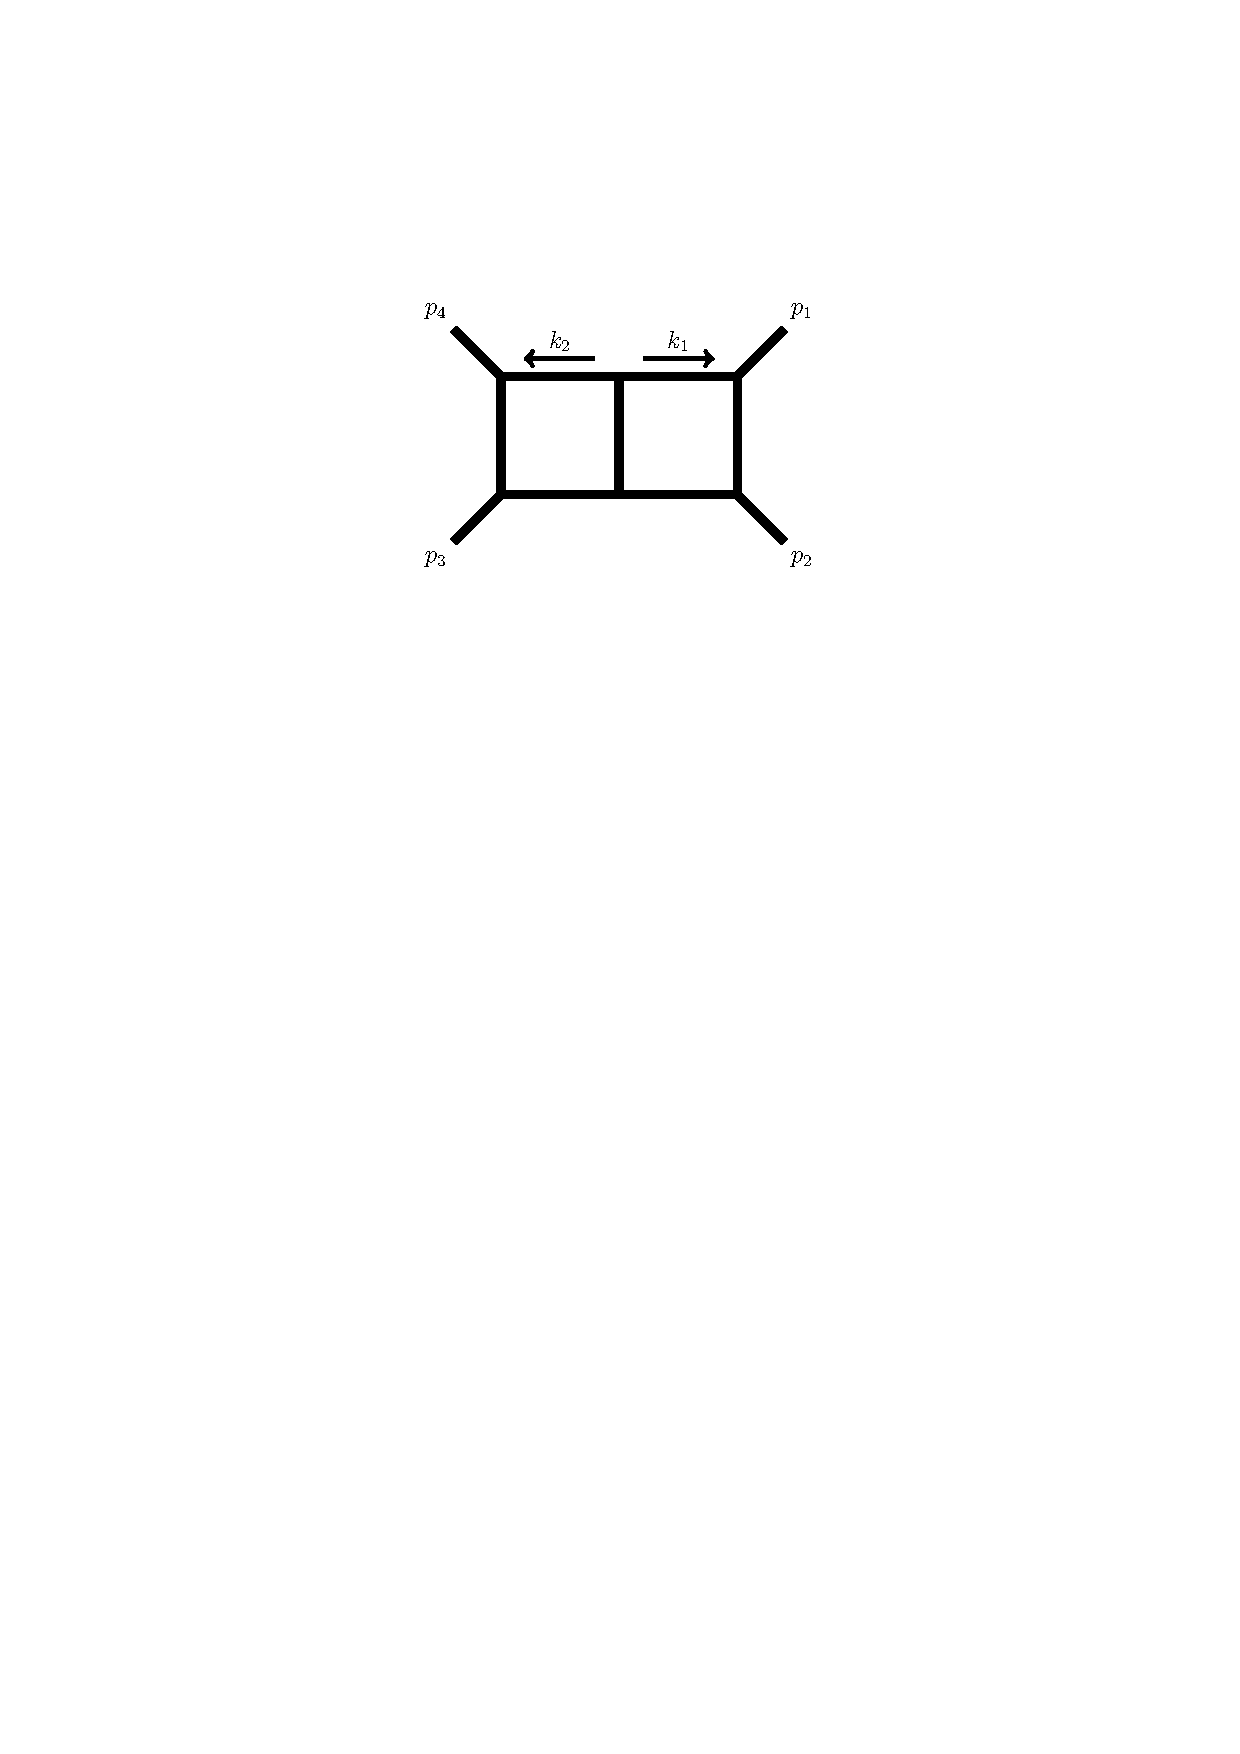
\includegraphics[width=0.4\textwidth]{ch3_loopamps/figures/dblbox-labels.pdf}
  \caption{A two-loop double box configuration.}
  \label{fig:2Ldblbox}
\end{figure}

We can run through a simple example to get a sense of the new features.
Consider a two-loop double box with seven massless propagators and massless external
legs as shown in figure~\ref{fig:2Ldblbox}. The propagators can be written in
terms of scalar products which are linear in the loop momenta $k_i\cdot p_j$, and three
scalar products quadratic in the loop momenta: $k_1^2$, $k_2^2$ and $k_1 \cdot k_2$. The
linear scalar products can be written as the difference of two inverse
propagators. The list of all possible scalar products $k_i \cdot \vec{v}_{j}$, where $\vec{v}^{\mu}$ is a
spanning set of momenta such as $\vec{v}^{\mu} = \{p_1^{\mu},p_2^{\mu},p_4^{\mu},\omega^{\mu}\}$, can then be
separated into the groups of 1) \emph{reducible scalar products}, that can be
written as the difference of propagators (plus functions of the external kinematic invariants), and 2) a set of four
irreducible scalar products (ISPs), for example $k_1\cdot p_4$, $k_2\cdot p_1$, $k_1\cdot\omega$,
and $k_2\cdot\omega$. Being more explicit, we decompose the loop momenta into transverse spaces,
\begin{align}
  k_i^\mu = k^\mu_{i,\parallel} + (k_i\cdot\omega)\,\omega^\mu \,.
\end{align}
The constraints on the scalar products $k_i\cdot p_j$ fix $k^\mu_{i,\parallel}$, which becomes a function of the two ISPs $k_1\cdot p_4$ and $k_2\cdot p_1$.
The remaining on-shell constraints for $k_1^2=0$, $k_2^2=0$ and $k_1 \cdot k_2=0$ can now be recast into conditions on all four ISPs,
\begin{align}
  &f_{11}(k_1\cdot p_4, k_2\cdot p_1) + (k_1\cdot\omega)^2 = 0 \,, \\
  &f_{22}(k_1\cdot p_4, k_2\cdot p_1) + (k_2\cdot\omega)^2 = 0 \,, \\
  &f_{12}(k_1\cdot p_4, k_2\cdot p_1) + (k_1\cdot\omega)(k_2\cdot\omega) = 0 \,,
\end{align}
where $f_{ij} = \mathcal{C}_{\rm double-box}(k_{1,\parallel}\cdot k_{2,\parallel})/\omega^2$ with $\mathcal{C}_{\rm double-box}$ indicating the hepta-cut.
The irreducible numerator $\Delta_{\rm double-box}(k_1\cdot p_4, k_2\cdot p_1,
k_1\cdot\omega, k_2\cdot\omega)$ may then be constructed by forming a general
polynomial of rank four\footnote{For QCD the maximum rank appearing in Feynman
diagrams in the Feynman gauge is four, in different theories a higher degree polynomial maybe necessary.} in the four ISPs and then removing the (multi-variate)
constraints through polynomial division. This operation involves the
computation of a Gr\"{o}bner basis, which can be computationally expensive but for
the construction of a general basis is unlikely to present a
bottleneck. In this case a suitable basis can be found to be~\cite{ch3_Badger:2012dp}
\begin{align}
& \Delta_{\rm double-box}(k_1\cdot p_4, k_2\cdot p_1, k_1\cdot\omega, k_2\cdot\omega) =
    c_0 \nonumber\\
    & \hspace{0.4cm}
    % rank 1
    + c_1 (k_1\cdot p_4)
    + c_2 (k_2\cdot p_1)
    % rank 2
    + c_3 (k_1\cdot p_4)^2
    + c_4 (k_2\cdot p_1)^2
    + c_5 (k_1\cdot p_4)(k_2\cdot p_1)\nonumber\\
    & \hspace{0.4cm}
    % rank 2
    + c_6 (k_1\cdot p_4)^3
    + c_7 (k_1\cdot p_4)(k_2\cdot p_1)^2
    + c_8 (k_1\cdot p_4)(k_2\cdot p_1)^2
    + c_9 (k_2\cdot p_1)^3\nonumber\\
    & \hspace{0.4cm}
    % rank 4
    + c_{10} (k_1\cdot p_4)^4
    + c_{11} (k_1\cdot p_4)^3 (k_2\cdot p_1)
    + c_{12} (k_1\cdot p_4) (k_2\cdot p_1)^3
    + c_{13} (k_2\cdot p_1)^4 \nonumber\\
    & \hspace{0.4cm}
    + \text{spurious terms} \,.
\end{align}
The additional tensor integrals can be reduced to a smaller basis of integrals
by the use of integration-by-parts identities, which will be a main topic in the
next chapter. In this case it turns out that only two of these integrals can
actually be considered independent. While the determination of
the integrand basis can be useful, for current state-of-the art problems the
integration-by-parts system presents a considerable computational bottleneck.

\begin{thebibliography}{99.}
%\cite{Sterman:1993hfp}
\bibitem{ch3_Sterman:1993hfp}
G.~F.~Sterman,
``An Introduction to quantum field theory,''
Cambridge University Press, 1993,
ISBN 978-0-521-31132-8.

%\cite{Peskin:1995ev}
\bibitem{ch3_Peskin:1995ev}
M.~E.~Peskin and D.~V.~Schroeder,
``An Introduction to quantum field theory,''
Addison-Wesley, 1995,
ISBN 978-0-201-50397-5.

%\cite{Schwartz:2014sze}
\bibitem{ch3_Schwartz:2014sze}
M.~D.~Schwartz,
``Quantum Field Theory and the Standard Model,''
Cambridge University Press, 2014,
ISBN 978-1-107-03473-0, 978-1-107-03473-0.

%\cite{Agarwal:2021ais}
\bibitem{ch3_Agarwal:2021ais}
N.~Agarwal, L.~Magnea, C.~Signorile-Signorile and A.~Tripathi,
``The infrared structure of perturbative gauge theories,''
Phys. Rept. \textbf{994} (2023), 1-120
doi:10.1016/j.physrep.2022.10.001
[arXiv:2112.07099 [hep-ph]].

%\cite{Dixon:1996wi}
\bibitem{ch3_Dixon:1996wi}
L.~J.~Dixon,
``Calculating scattering amplitudes efficiently,''
[arXiv:hep-ph/9601359 [hep-ph]].

%\cite{Dixon:2013uaa}
\bibitem{ch3_Dixon:2013uaa}
L.~J.~Dixon,
``A brief introduction to modern amplitude methods,''
doi:10.5170/CERN-2014-008.31
[arXiv:1310.5353 [hep-ph]].

%\cite{Ellis:2011cr}
\bibitem{ch3_Ellis:2011cr}
R.~K.~Ellis, Z.~Kunszt, K.~Melnikov and G.~Zanderighi,
``One-loop calculations in quantum field theory: from Feynman diagrams to unitarity cuts,''
Phys. Rept. \textbf{518} (2012), 141-250
doi:10.1016/j.physrep.2012.01.008
[arXiv:1105.4319 [hep-ph]].

%\cite{Cutkosky:1960sp}
\bibitem{ch3_Cutkosky:1960sp}
R.~E.~Cutkosky,
``Singularities and discontinuities of Feynman amplitudes,''
J. Math. Phys. \textbf{1} (1960), 429-433
doi:10.1063/1.1703676.

%\cite{Eden:1966dnq}
\bibitem{ch3_Eden:1966dnq}
R.~J.~Eden, P.~V.~Landshoff, D.~I.~Olive and J.~C.~Polkinghorne,
``The analytic S-matrix,''
Cambridge Univ. Press, 1966,
ISBN 978-0-521-04869-9.

%\cite{Bern:1994zx}
\bibitem{ch3_Bern:1994zx}
Z.~Bern, L.~J.~Dixon, D.~C.~Dunbar and D.~A.~Kosower,
``One loop n point gauge theory amplitudes, unitarity and collinear limits,''
Nucl. Phys. B \textbf{425} (1994), 217-260
doi:10.1016/0550-3213(94)90179-1
[arXiv:hep-ph/9403226 [hep-ph]].

%\cite{Passarino:1978jh}
\bibitem{ch3_Passarino:1978jh}
G.~Passarino and M.~J.~G.~Veltman,
``One Loop Corrections for e+ e- Annihilation Into mu+ mu- in the Weinberg Model,''
Nucl. Phys. B \textbf{160} (1979), 151-207
doi:10.1016/0550-3213(79)90234-7.

%\cite{vanNeerven:1983vr}
\bibitem{ch3_vanNeerven:1983vr}
W.~L.~van Neerven and J.~A.~M.~Vermaseren,
``Large loop integrals,''
Phys. Lett. B \textbf{137} (1984), 241-244
doi:10.1016/0370-2693(84)90237-5.

%\cite{Baikov:1996rk}
\bibitem{ch3_Baikov:1996rk}
P.~A.~Baikov,
``Explicit solutions of the three loop vacuum integral recurrence relations,''
Phys. Lett. B \textbf{385} (1996), 404-410
doi:10.1016/0370-2693(96)00835-0
[arXiv:hep-ph/9603267 [hep-ph]].

%\cite{Mastrolia:2016dhn}
\bibitem{ch3_Mastrolia:2016dhn}
P.~Mastrolia, T.~Peraro and A.~Primo,
``Adaptive Integrand Decomposition in parallel and orthogonal space,''
JHEP \textbf{08} (2016), 164
doi:10.1007/JHEP08(2016)164
[arXiv:1605.03157 [hep-ph]].

%\cite{Ossola:2006us}
\bibitem{ch3_Ossola:2006us}
G.~Ossola, C.~G.~Papadopoulos and R.~Pittau,
``Reducing full one-loop amplitudes to scalar integrals at the integrand level,''
Nucl. Phys. B \textbf{763} (2007), 147-169
doi:10.1016/j.nuclphysb.2006.11.012
[arXiv:hep-ph/0609007 [hep-ph]].

%\cite{Ellis:2008ir}
\bibitem{ch3_Ellis:2008ir}
R.~K.~Ellis, W.~T.~Giele, Z.~Kunszt and K.~Melnikov,
``Masses, fermions and generalized $D$-dimensional unitarity,''
Nucl. Phys. B \textbf{822} (2009), 270-282
doi:10.1016/j.nuclphysb.2009.07.023
[arXiv:0806.3467 [hep-ph]].

%\cite{Britto:2011cr}
\bibitem{ch3_Britto:2011cr}
R.~Britto and E.~Mirabella,
``External leg corrections in the unitarity method,''
JHEP \textbf{01} (2012), 045
doi:10.1007/JHEP01(2012)045
[arXiv:1109.5106 [hep-ph]].

%\cite{Badger:2017gta}
\bibitem{ch3_Badger:2017gta}
S.~Badger, C.~Br\o{}nnum-Hansen, F.~Buciuni and D.~O'Connell,
``A unitarity compatible approach to one-loop amplitudes with massive fermions,''
JHEP \textbf{06} (2017), 141
doi:10.1007/JHEP06(2017)141
[arXiv:1703.05734 [hep-ph]].

%\cite{Bern:1995db}
\bibitem{ch3_Bern:1995db}
Z.~Bern and A.~G.~Morgan,
``Massive loop amplitudes from unitarity,''
Nucl. Phys. B \textbf{467} (1996), 479-509
doi:10.1016/0550-3213(96)00078-8
[arXiv:hep-ph/9511336 [hep-ph]].

%\cite{Berger:2008sj}
\bibitem{ch3_Berger:2008sj}
C.~F.~Berger, Z.~Bern, L.~J.~Dixon, F.~Febres Cordero, D.~Forde, H.~Ita, D.~A.~Kosower and D.~Maitre,
``An Automated Implementation of On-Shell Methods for One-Loop Amplitudes,''
Phys. Rev. D \textbf{78} (2008), 036003
doi:10.1103/PhysRevD.78.036003
[arXiv:0803.4180 [hep-ph]].

%\cite{Giele:2008bc}
\bibitem{ch3_Giele:2008bc}
W.~T.~Giele and G.~Zanderighi,
``On the Numerical Evaluation of One-Loop Amplitudes: The Gluonic Case,''
JHEP \textbf{06} (2008), 038
doi:10.1088/1126-6708/2008/06/038
[arXiv:0805.2152 [hep-ph]].

%\cite{Hirschi:2011pa}
\bibitem{ch3_Hirschi:2011pa}
V.~Hirschi, R.~Frederix, S.~Frixione, M.~V.~Garzelli, F.~Maltoni and R.~Pittau,
``Automation of one-loop QCD corrections,''
JHEP \textbf{05} (2011), 044
doi:10.1007/JHEP05(2011)044
[arXiv:1103.0621 [hep-ph]].

%\cite{Bevilacqua:2011xh}
\bibitem{ch3_Bevilacqua:2011xh}
G.~Bevilacqua, M.~Czakon, M.~V.~Garzelli, A.~van Hameren, A.~Kardos, C.~G.~Papadopoulos, R.~Pittau and M.~Worek,
``HELAC-NLO,''
Comput. Phys. Commun. \textbf{184} (2013), 986-997
doi:10.1016/j.cpc.2012.10.033
[arXiv:1110.1499 [hep-ph]].

%\cite{Badger:2012pg}
\bibitem{ch3_Badger:2012pg}
S.~Badger, B.~Biedermann, P.~Uwer and V.~Yundin,
``Numerical evaluation of virtual corrections to multi-jet production in massless QCD,''
Comput. Phys. Commun. \textbf{184} (2013), 1981-1998
doi:10.1016/j.cpc.2013.03.018
[arXiv:1209.0100 [hep-ph]].

%\cite{GoSam:2014iqq}
\bibitem{ch3_GoSam:2014iqq}
G.~Cullen \textit{et al.} [GoSam],
``G$\scriptsize{O}$S$\scriptsize{AM}$-2.0: a tool for automated one-loop calculations within the Standard Model and beyond,''
Eur. Phys. J. C \textbf{74} (2014) no.8, 3001
doi:10.1140/epjc/s10052-014-3001-5
[arXiv:1404.7096 [hep-ph]].

%\cite{Actis:2016mpe}
\bibitem{ch3_Actis:2016mpe}
S.~Actis, A.~Denner, L.~Hofer, J.~N.~Lang, A.~Scharf and S.~Uccirati,
``RECOLA: REcursive Computation of One-Loop Amplitudes,''
Comput. Phys. Commun. \textbf{214} (2017), 140-173
doi:10.1016/j.cpc.2017.01.004
[arXiv:1605.01090 [hep-ph]].

%\cite{Buccioni:2019sur}
\bibitem{ch3_Buccioni:2019sur}
F.~Buccioni \textit{et al.} [OpenLoops 2],
``OpenLoops 2,''
Eur. Phys. J. C \textbf{79} (2019) no.10, 866
doi:10.1140/epjc/s10052-019-7306-2
[arXiv:1907.13071 [hep-ph]].

%\cite{Giele:2008ve}
\bibitem{ch3_Giele:2008ve}
W.~T.~Giele, Z.~Kunszt and K.~Melnikov,
``Full one-loop amplitudes from tree amplitudes,''
JHEP \textbf{04} (2008), 049
doi:10.1088/1126-6708/2008/04/049
[arXiv:0801.2237 [hep-ph]].

%\cite{Bern:2010qa}
\bibitem{ch3_Bern:2010qa}
Z.~Bern, J.~J.~Carrasco, T.~Dennen, Y.~t.~Huang and H.~Ita,
``Generalized Unitarity and Six-Dimensional Helicity,''
Phys. Rev. D \textbf{83} (2011), 085022
doi:10.1103/PhysRevD.83.085022
[arXiv:1010.0494 [hep-th]].

%\cite{Forde:2007mi}
\bibitem{ch3_Forde:2007mi}
D.~Forde,
``Direct extraction of one-loop integral coefficients,''
Phys. Rev. D \textbf{75} (2007), 125019
doi:10.1103/PhysRevD.75.125019
[arXiv:0704.1835 [hep-ph]].

%\cite{Badger:2008cm}
\bibitem{ch3_Badger:2008cm}
S.~D.~Badger,
``Direct Extraction Of One Loop Rational Terms,''
JHEP \textbf{01} (2009), 049
doi:10.1088/1126-6708/2009/01/049
[arXiv:0806.4600 [hep-ph]].

%\cite{Mastrolia:2008jb}
\bibitem{ch3_Mastrolia:2008jb}
P.~Mastrolia, G.~Ossola, C.~G.~Papadopoulos and R.~Pittau,
``Optimizing the Reduction of One-Loop Amplitudes,''
JHEP \textbf{06} (2008), 030
doi:10.1088/1126-6708/2008/06/030
[arXiv:0803.3964 [hep-ph]].

%\cite{Bern:1990ux}
\bibitem{ch3_Bern:1990ux}
Z.~Bern and D.~A.~Kosower,
``Color decomposition of one loop amplitudes in gauge theories,''
Nucl. Phys. B \textbf{362} (1991), 389-448
doi:10.1016/0550-3213(91)90567-H.

%\cite{Bern:1994fz}
\bibitem{ch3_Bern:1994fz}
Z.~Bern, L.~J.~Dixon and D.~A.~Kosower,
``One loop corrections to two quark three gluon amplitudes,''
Nucl. Phys. B \textbf{437} (1995), 259-304
doi:10.1016/0550-3213(94)00542-M
[arXiv:hep-ph/9409393 [hep-ph]].

%\cite{Hodges:2009hk}
\bibitem{ch3_Hodges:2009hk}
A.~Hodges,
``Eliminating spurious poles from gauge-theoretic amplitudes,''
JHEP \textbf{05} (2013), 135
doi:10.1007/JHEP05(2013)135
[arXiv:0905.1473 [hep-th]].

%\cite{Peraro:2016wsq}
\bibitem{ch3_Peraro:2016wsq}
T.~Peraro,
``Scattering amplitudes over finite fields and multivariate functional reconstruction,''
JHEP \textbf{12} (2016), 030
doi:10.1007/JHEP12(2016)030
[arXiv:1608.01902 [hep-ph]].

%\cite{Peraro:2019svx}
\bibitem{ch3_Peraro:2019svx}
T.~Peraro,
``FiniteFlow: multivariate functional reconstruction using finite fields and dataflow graphs,''
JHEP \textbf{07} (2019), 031
doi:10.1007/JHEP07(2019)031
[arXiv:1905.08019 [hep-ph]].

%\cite{Elvang:2013cua}
\bibitem{ch3_Elvang:2013cua}
H.~Elvang and Y.~t.~Huang,
``Scattering Amplitudes,''
[arXiv:1308.1697 [hep-th]].

%\cite{Badger:2012dp}
\bibitem{ch3_Badger:2012dp}
S.~Badger, H.~Frellesvig and Y.~Zhang,
``Hepta-Cuts of Two-Loop Scattering Amplitudes,''
JHEP \textbf{04} (2012), 055
doi:10.1007/JHEP04(2012)055
[arXiv:1202.2019 [hep-ph]].

\bibitem{website-ch3}
\href{https://scattering-amplitudes.mpp.mpg.de/scattering-amplitudes-in-qft/Exercises/}{https://scattering-amplitudes.mpp.mpg.de/scattering-amplitudes-in-qft/Exercises/}.
\end{thebibliography}
